\chapter{Instrumental Characterization of BLAST-TNG}\label{blast_data}

The following sections describe the characterization of the instrumental performance of BLAST-TNG in the lead-up to the 2018/2019 launch attempt from NASA's Long Duration Balloon site (LDB) in Antarctica. Because the camera contains over 2,500 polarization sensitive pixels distributed over three wavebands, it would not be feasible to describe the individual performance of each pixel within this document. Instead, we present a detailed data reduction for a single pixel, which is then extended to statistical results which summarize the overall performance of each BLAST-TNG band. The instrumental performance is characterized by numerous parameters, many of which are interdependent and can not be directly measured. Instead, they must be inferred from the results of empirical measurements, which in some cases can be checked against a model, such as the one presented in Chapter~\ref{kid_model}.

Out of all of the instrumental parameters that could be examined, a small number of them directly determine how well the camera will perform in terms of its mapping speed and on-sky sensitivity to sub-mm intensity and polarization. These parameters are the detector yields and NEP or NET (sensitivity), optical efficiency, passband shapes and polarization efficiencies. The in-flight performance is also directly related to the operation of the detector readout. For example, to utilize the full dynamic range of each detector during flight will require that the readout probe tones be periodically retuned in frequency and amplitude. Notes on readout operation are interspersed with the following description of how each of the aforementioned parameters has been estimated.

The chapter is organized as follows:

\begin{itemize}[nosep]
  \item Section~\ref{sweeps} introduces detector frequency sweeps, frequency-domain channel identification, and detector yields.
  \item Section~\ref{timestreams} introduces the raw $I/Q$ timestreams which are generated by the readout, and how they are calibrated into frequency units which are proportional to absorbed optical power.
  \item Section~\ref{responsivities} discusses the responsivities to absorbed optical power and changes in base temperature.
  \item Section~\ref{sensitivity} presents sensitivity estimates for each band (NEP) and describes how these estimates are made using a combination of sweeps, timestreams and optical tests.
  \item In Section~\ref{applying model} we compare the measured data for a single channel from the 350~$\upmu$m and 250W arrays to results from the parametric LEKID model presented in Chapter~\ref{kid_model}.
  \item In Section~\ref{histograms} we present histograms showing the distribution of important detector parameters for each of the five BLAST-TNG detector arrays.
  \item Section~\ref{optical tests} presents the data reduction and results of passband mapping (Section~\ref{fts}) and polarization efficiency (Section~\ref{pol eff}).
\end{itemize}

The data used in the following analysis was mostly acquired in May, 2018 (Philadelphia, PA), July, 2018 (NASA's Columbia Scientific Ballooning Facility (CSBF) Palestine, Texas), and winter 2018/2019 (NASA Long Duration Balloon facility (LDB), Antarctica).

\section{Detector Sweeps}\label{sweeps}

The BLAST-TNG detectors are distributed between five LEKID arrays, with one for the 350 and 500~$\upmu$m bands, and three for the 250~$\upmu$m. The three 250~$\upmu$m arrays (hereafter referred to as the 250U, 250V and 250W) reside on the same chip, but are read out independently. The 250V RF-chain malfunctioned during the pre-flight instrument integration at LDB, and we therefore do not present results for this channel from the Antarctic (`ice') campaign.

Every test of the detectors begins with a frequency sweep of the full 512~MHz RF-bandwidth occupied by each detector array. If the resonator frequencies are not known ahead of time, or have drifted by more than $\sim$1 resonator linewidth, the wide sweep is used to identify the channel frequencies (see Section~\ref{KID-finding}). A wide sweep (sometimes referred to as a `VNA' sweep) is performed by sweeping the 1,000 tone evenly-spaced search-comb over the 500~kHz gap between tones. The multitone comb is swept by stepping the local oscillator (LO) from one end of the 500~kHz gap to the other in frequency steps of $\approx$ 1~kHz. At each step, $I/Q$ data is saved to disk and co-added, with the number of data points taken at each frequency typically being $\sim$20. The wide-sweeps take $\sim$30 seconds to complete. Plotted as a function of RF-frequency, the data shows $\gls{S21}V_{\mathrm{in}}$ of the detector readout chain (hereafter simply referred to as \gls{S21}), where $V_{\mathrm{in}}$ is the amplitude of the probe-tone comb at the output of the ROACH2 digital-to-analog converters (DACs).

\subsection{The Wide-sweep Frequency Response}\label{freq response}

Figures~\ref{fig:350 wide sweep} and Figures~\ref{fig:350 zoom} show an overlay of two example sweeps of the 350~$\upmu$m array. The blue sweep was taken in May, 2018, and the orange trace was taken in July, 2018. The blue sweep shows the raw (uncorrected) frequency response of the readout system and detector chain, whereas the orange trace was produced by applying several corrections to the readout probe tone amplitudes. The transfer function correction is described in Section~\ref{TRF}. Both sweeps were taken with the cryostat window exposed to the $\sim$300~K thermal radiation of the highbay. A (2.85\%) 4\% neutral-density filter (NDF) inside the receiver's cold-optics limits the optical power which reaches the detectors (after accounting for an instrumental optical efficiency \gls{opt_eff} of $\sim$30\%, and a detector efficiency \gls{det_eff} of $\sim$80\%) to $\sim$10~pW.

The frequency response (or transfer function) of the system contains information about the frequency response of every element in the detector chain. The primary contributors are the ROACH2 electronics, input and output side intermediate-frequency (IF) electronics, room-temperature as well as cryogenic cabling, the cryogenic low-noise amplifier (LNA) and the detector arrays themselves. In the frequency domain, the total system response is the product of the transfer function for each of the individual elements.

The envelope of the uncorrected \gls{S21} sweep contains several notable features:

\begin{itemize}[nosep]
  \item A gradual roll-off in power toward the band-edges.
  \item A steep roll-off in power at the band-edges.
  \item A deep null in the center of the band.
  \item A standing wave (ringing) pattern with a frequency of $\sim$30~MHz.
\end{itemize}

\begin{figure}[!htbp]
\centering
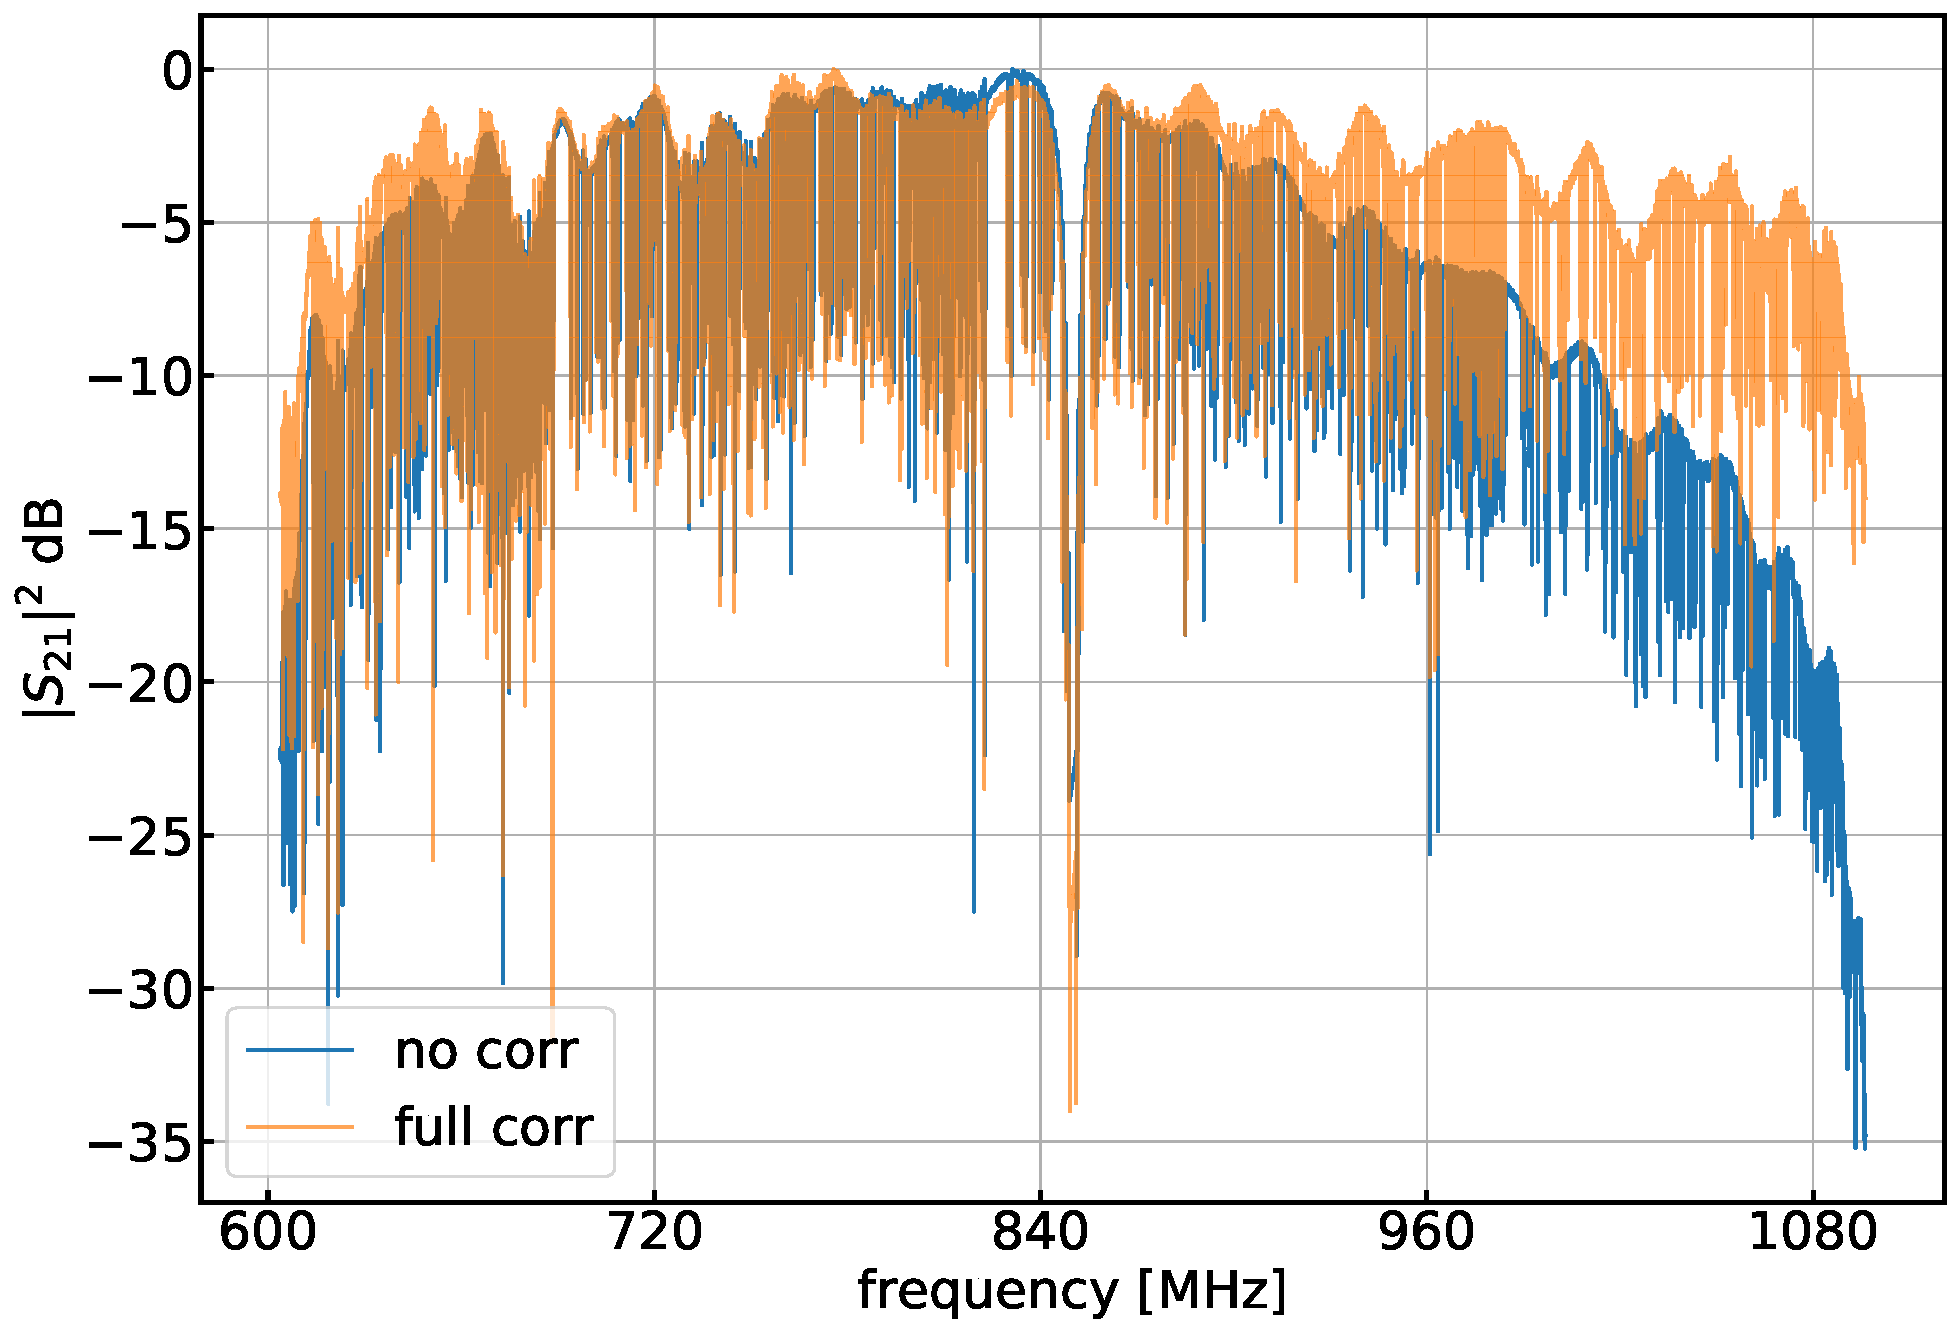
\includegraphics[width=\textwidth]{figures/blast_data/sweeps/350_wide_sweep}
\caption[~Comparison between raw and corrected wide-sweeps of the \macrocapwrap{350~$\upmu$m} array.]{Uncorrected (blue) and corrected (orange) ROACH2 wide-sweeps of the BLAST-TNG 350~$\upmu$m array.}
\label{fig:350 wide sweep}
\end{figure}

\begin{figure}[!htbp]
\centering
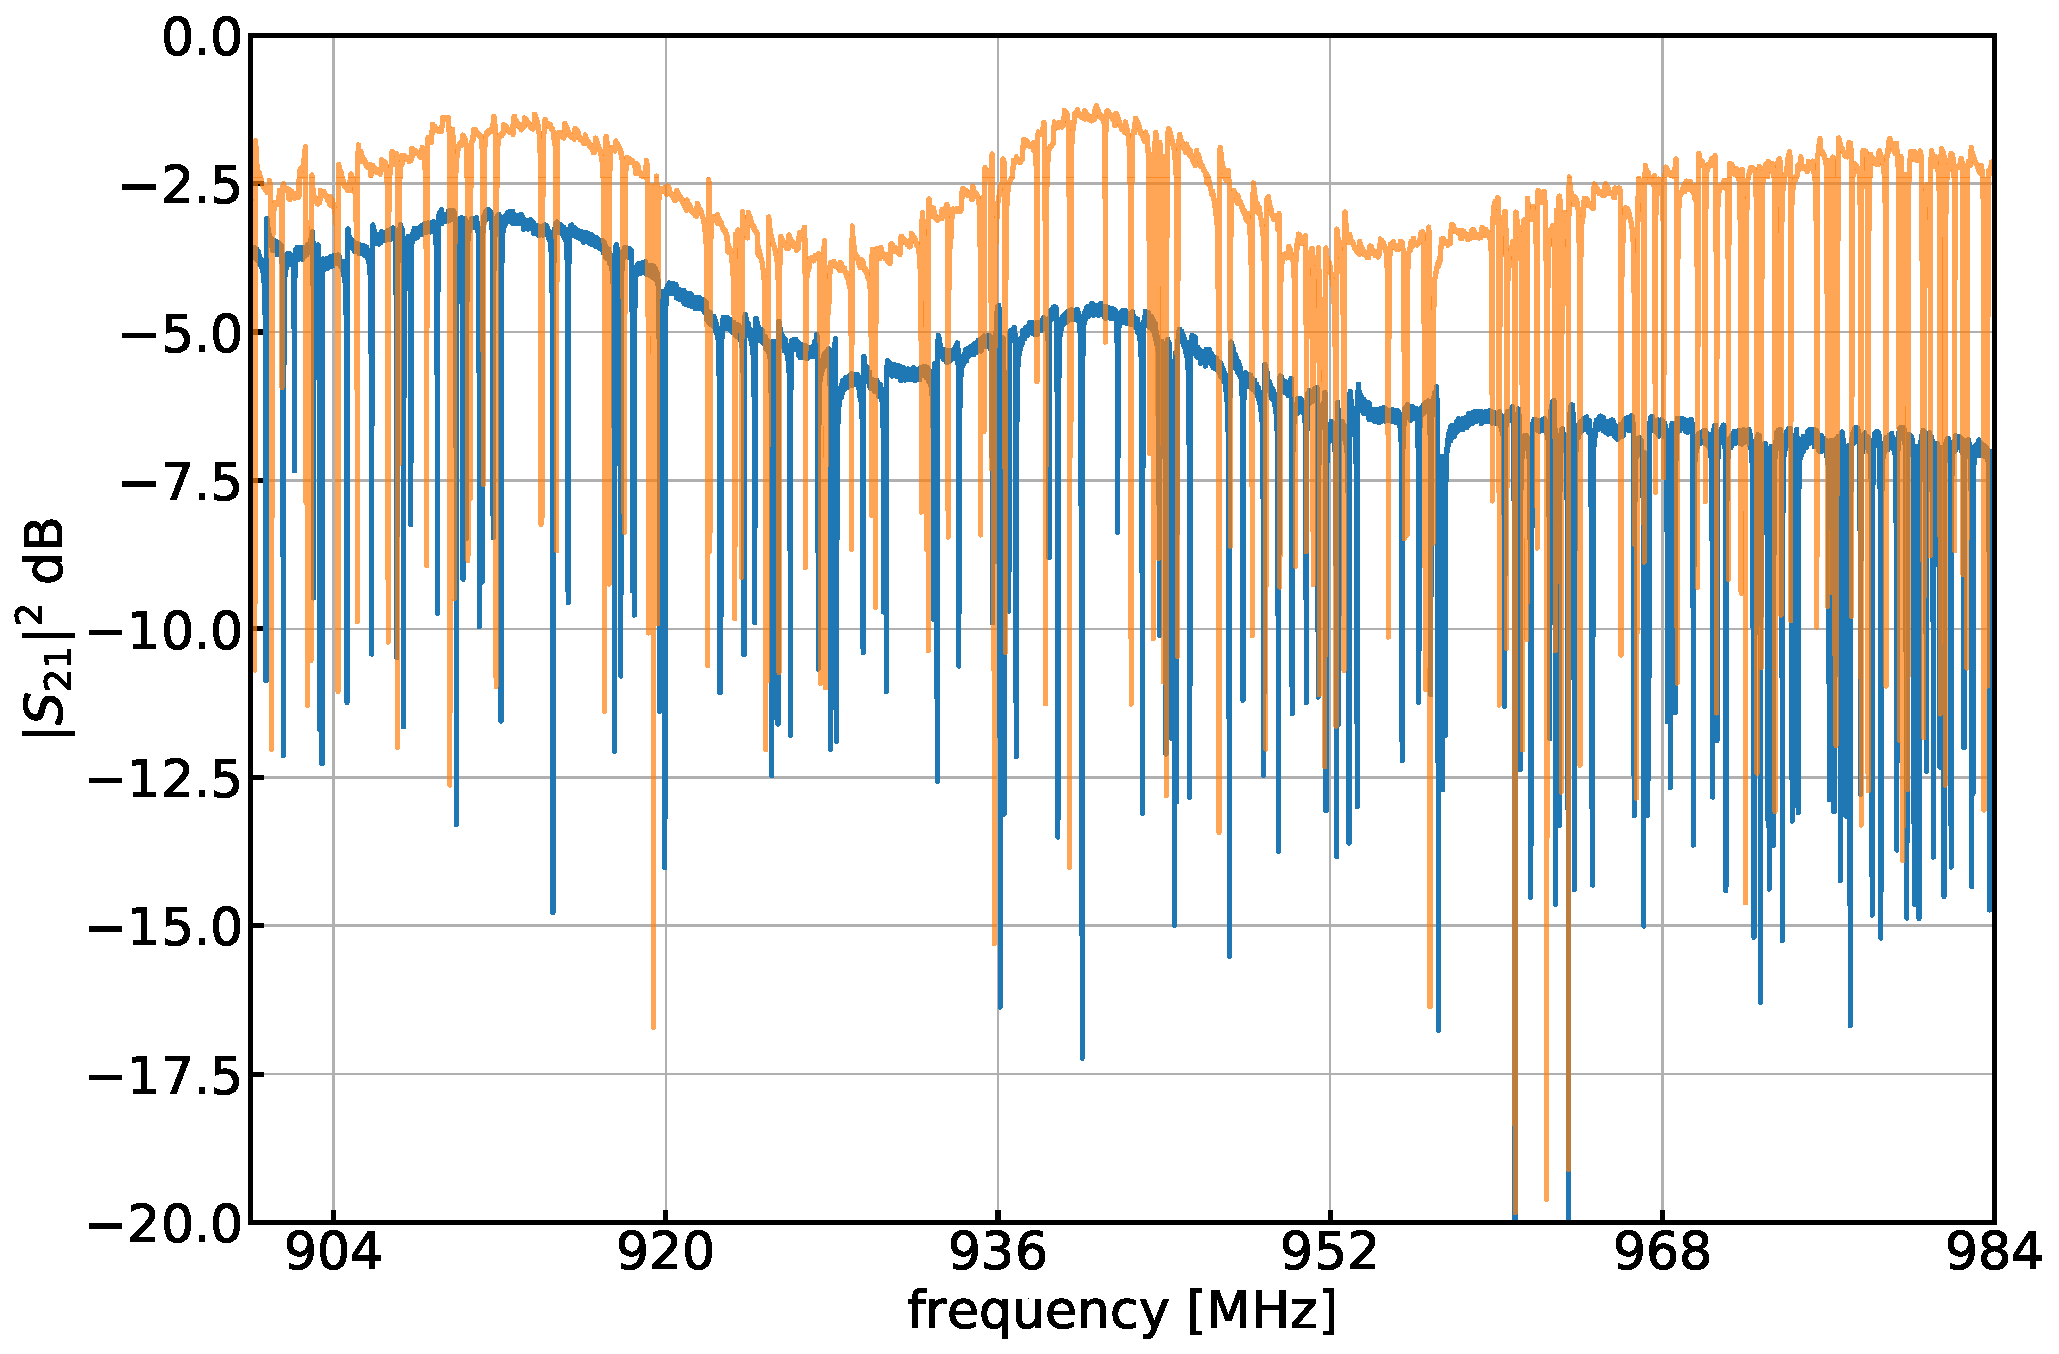
\includegraphics[width=\textwidth]{figures/blast_data/sweeps/350_wide_sweep_zoom}
\caption[~A zoomed-in region of an unprocessed and processed wide-sweep of the \macrocapwrap{350~$\upmu$m} array.]{A zoomed-in region of an unprocessed (blue) and processed (orange) wide-sweep of the 350~$\upmu$m array.}
\label{fig:350 zoom}
\end{figure}

The gradual roll-off in power toward the band-edges can be attributed to the MUSIC board's DAC frequency response, the LNA frequency response at low frequency ($\sim$500~MHz) as well as to the frequency response of modulator and demodulator (the demodulator contains 300~MHz low-pass filters). The steeper roll-off that begins at $\sim$15~MHz from the lower and upper band-edges is from the baseband anti-aliasing filters. The ringing pattern in the \gls{S21} envelope is due to a combination of the anti-aliasing filters and warm and cold cabling. The null in the center of the band is where the LO frequency is located. Typically, no probe tones are generated inside a 20~MHz band centered at the LO frequency.

The remaining features in the \gls{S21} trace shown in Figure~\ref{fig:350 wide sweep} are the individual resonator transfer functions. The 350~$\upmu$m array contains $\sim$750 resonators (within the readout band-- see Section~\ref{yields}). A small number of resonators with their horn antennas blocked off, known as $\textit{darks}$, have noticeably deeper resonances than the other detectors. The distribution of resonator dip-depths varies widely across the band. This spread is due to variations in several parameters, including intrinsic resonator quality factors, readout powers and optical loading. Much of the large scale variations in readout power can be corrected for by applying a global inverse transfer function to the probe comb. In addition to this, the tone power for each channel may be individually adjusted. The process of determining and applying the inverse transfer function correction is described in the following section.

\subsection{Transfer function Correction}\label{TRF}

As discussed in Section~\ref{freq response}, the uncorrected \gls{S21} frequency response revealed by the ROACH2 wide sweeps contain large scale features that may contribute to uneven detector performance across the band. Some of these features can be compensated for by applying an inverse transfer function to the amplitudes of the DAC probe comb. The goal of applying this correction is to correct for, as much as possible, any transfer function contributions from the input side of the detector chain (relative to the cryostat). All output side transfer functions (after and including the detectors) are left untouched. The components whose transfer functions will be corrected include the ROACH2 output-side electronics (both digital and analog) and any coaxial cables between the ROACH2 electronics and the detector arrays.

The output side system transfer function is measured by connecting the RF output of the ROACH2 IF electronics to a spectrum analyzer. The spectrum is then saved to disk, and interpolated in frequency as needed. Examples of the intermediate products used in the transfer function calculation are shown in Figure~\ref{fig:350 TRF}. The blue trace is the raw output of the RF modulator. A $\sim$10~dB roll-off is present between the center of the band and either band-edge. In addition to correcting for the envelope of the ROACH2 comb, a power ramp (shown as a green line) is added to the correction to compensate for frequency dependent loss in the cryostat cables. The inverse transfer function which is then applied to the DAC comb amplitudes is shown in orange.

The frequency-dependent cable loss which occurs inside the cryostat is visible in Figures~\ref{fig:VNA comp 350} to~\ref{fig:VNA comp 500}, which show \gls{S21} sweeps taken with a VNA (purple) compared to corrected ROACH2 \gls{S21} sweeps (orange) for each BLAST-TNG array. The cable loss is $\sim$10 dB across the readout-band. With the application of the inverse transfer function, much of the roll-off in the envelope of the frequency response is compensated for. For each array, a slightly different slope for the power ramp is used. An illustration of the effect of using different slope corrections for the 350~$\upmu$m array is shown in Figure~\ref{fig:trf slopes}, for slopes of 5, 8 and 10~dB (across the entire readout band).

\begin{figure}[!htbp]
\centering
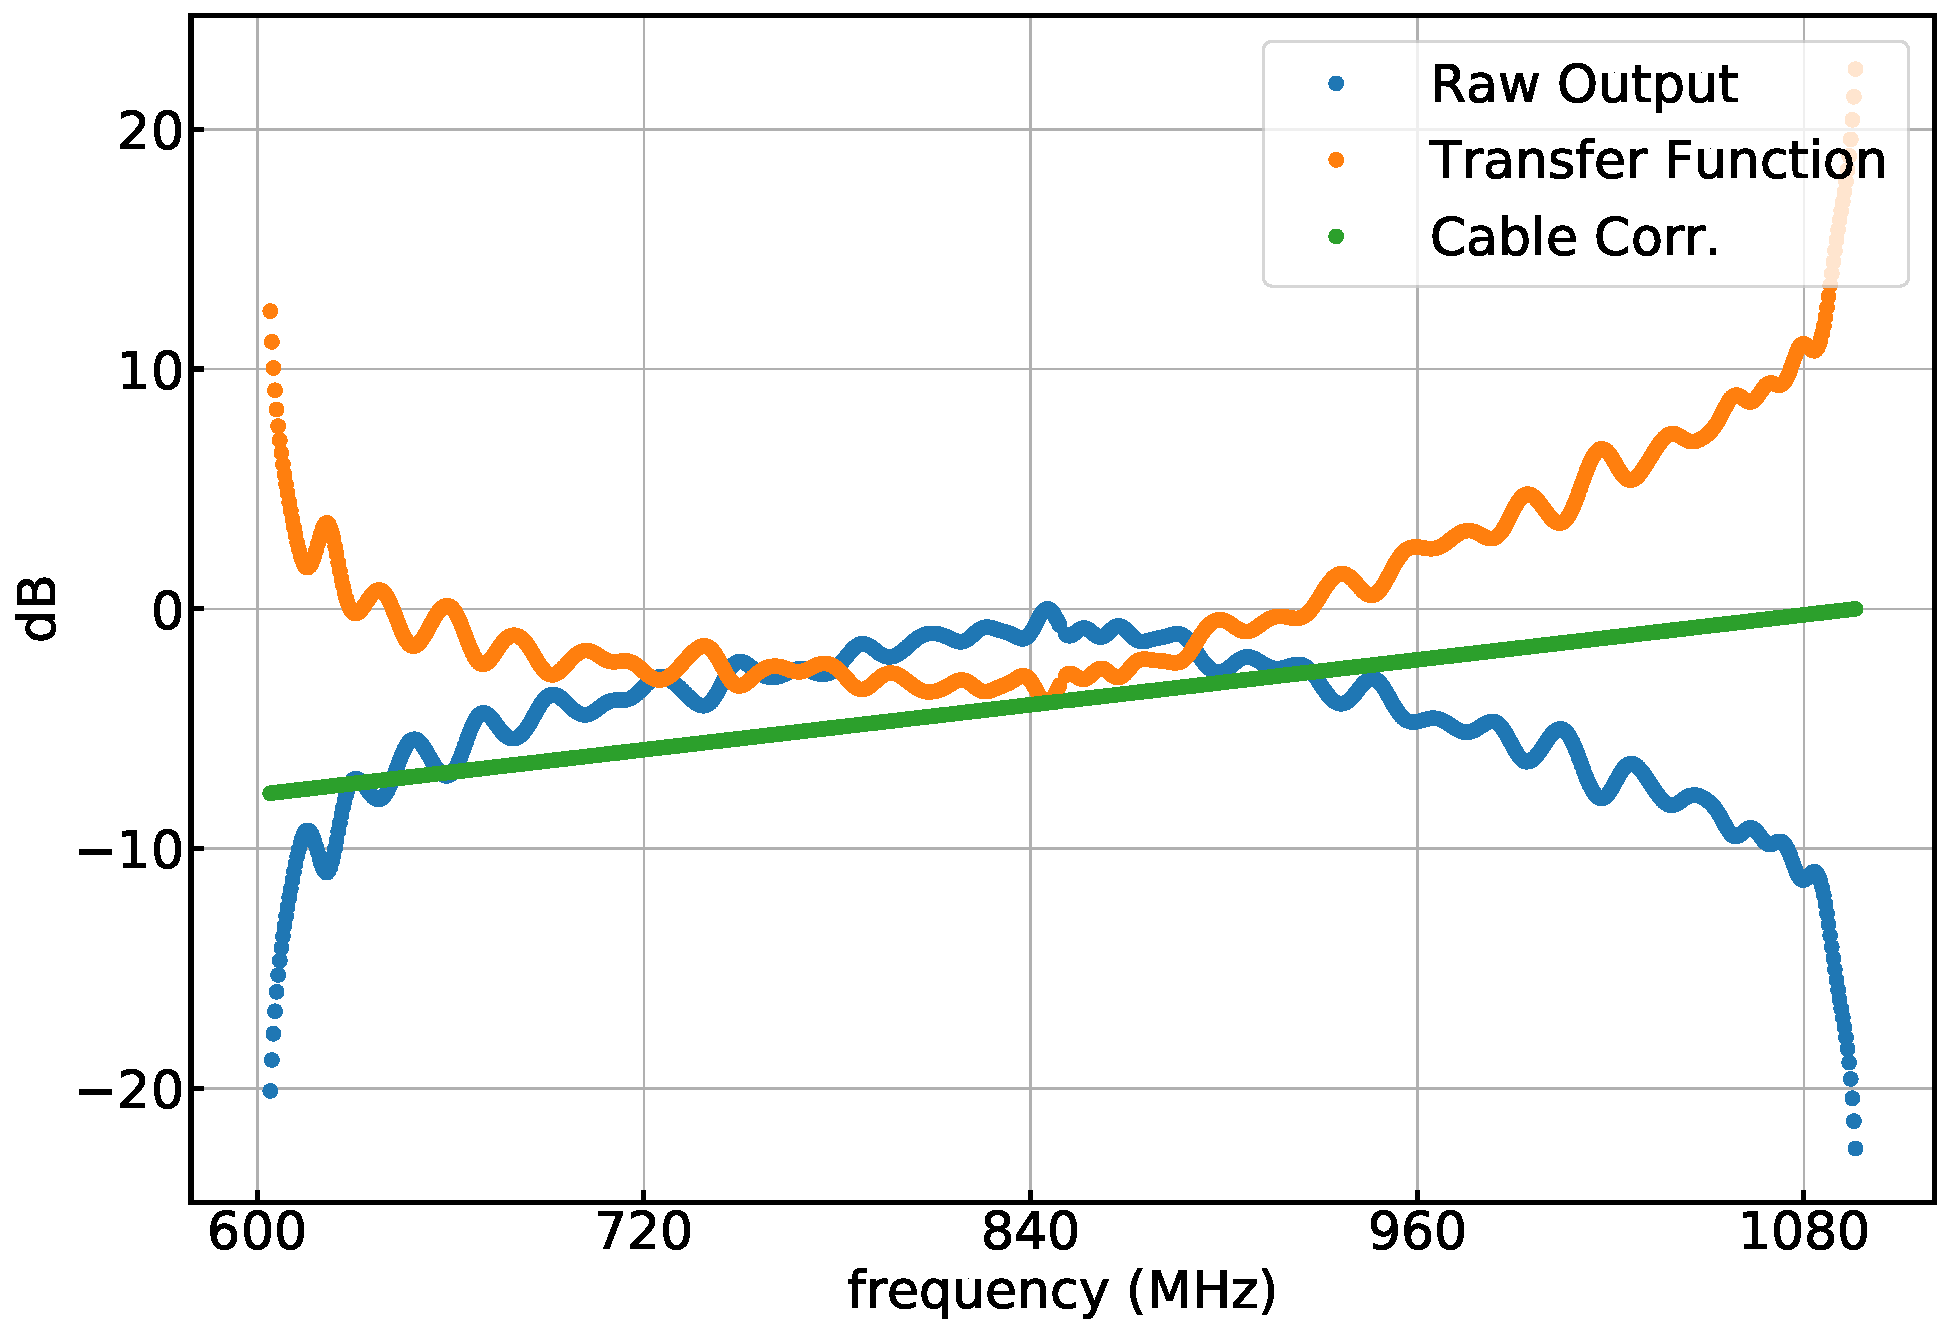
\includegraphics[width=\textwidth]{figures/blast_data/sweeps/r3_transfunc}
\caption[~Intermediate products used in the transfer function calculation for the \macrocapwrap{350~$\upmu$m} array.]{Intermediate products used in the transfer function calculation for the 350~$\upmu$m array.}
\label{fig:350 TRF}
\end{figure}

\begin{figure}[!htbp]
\centering
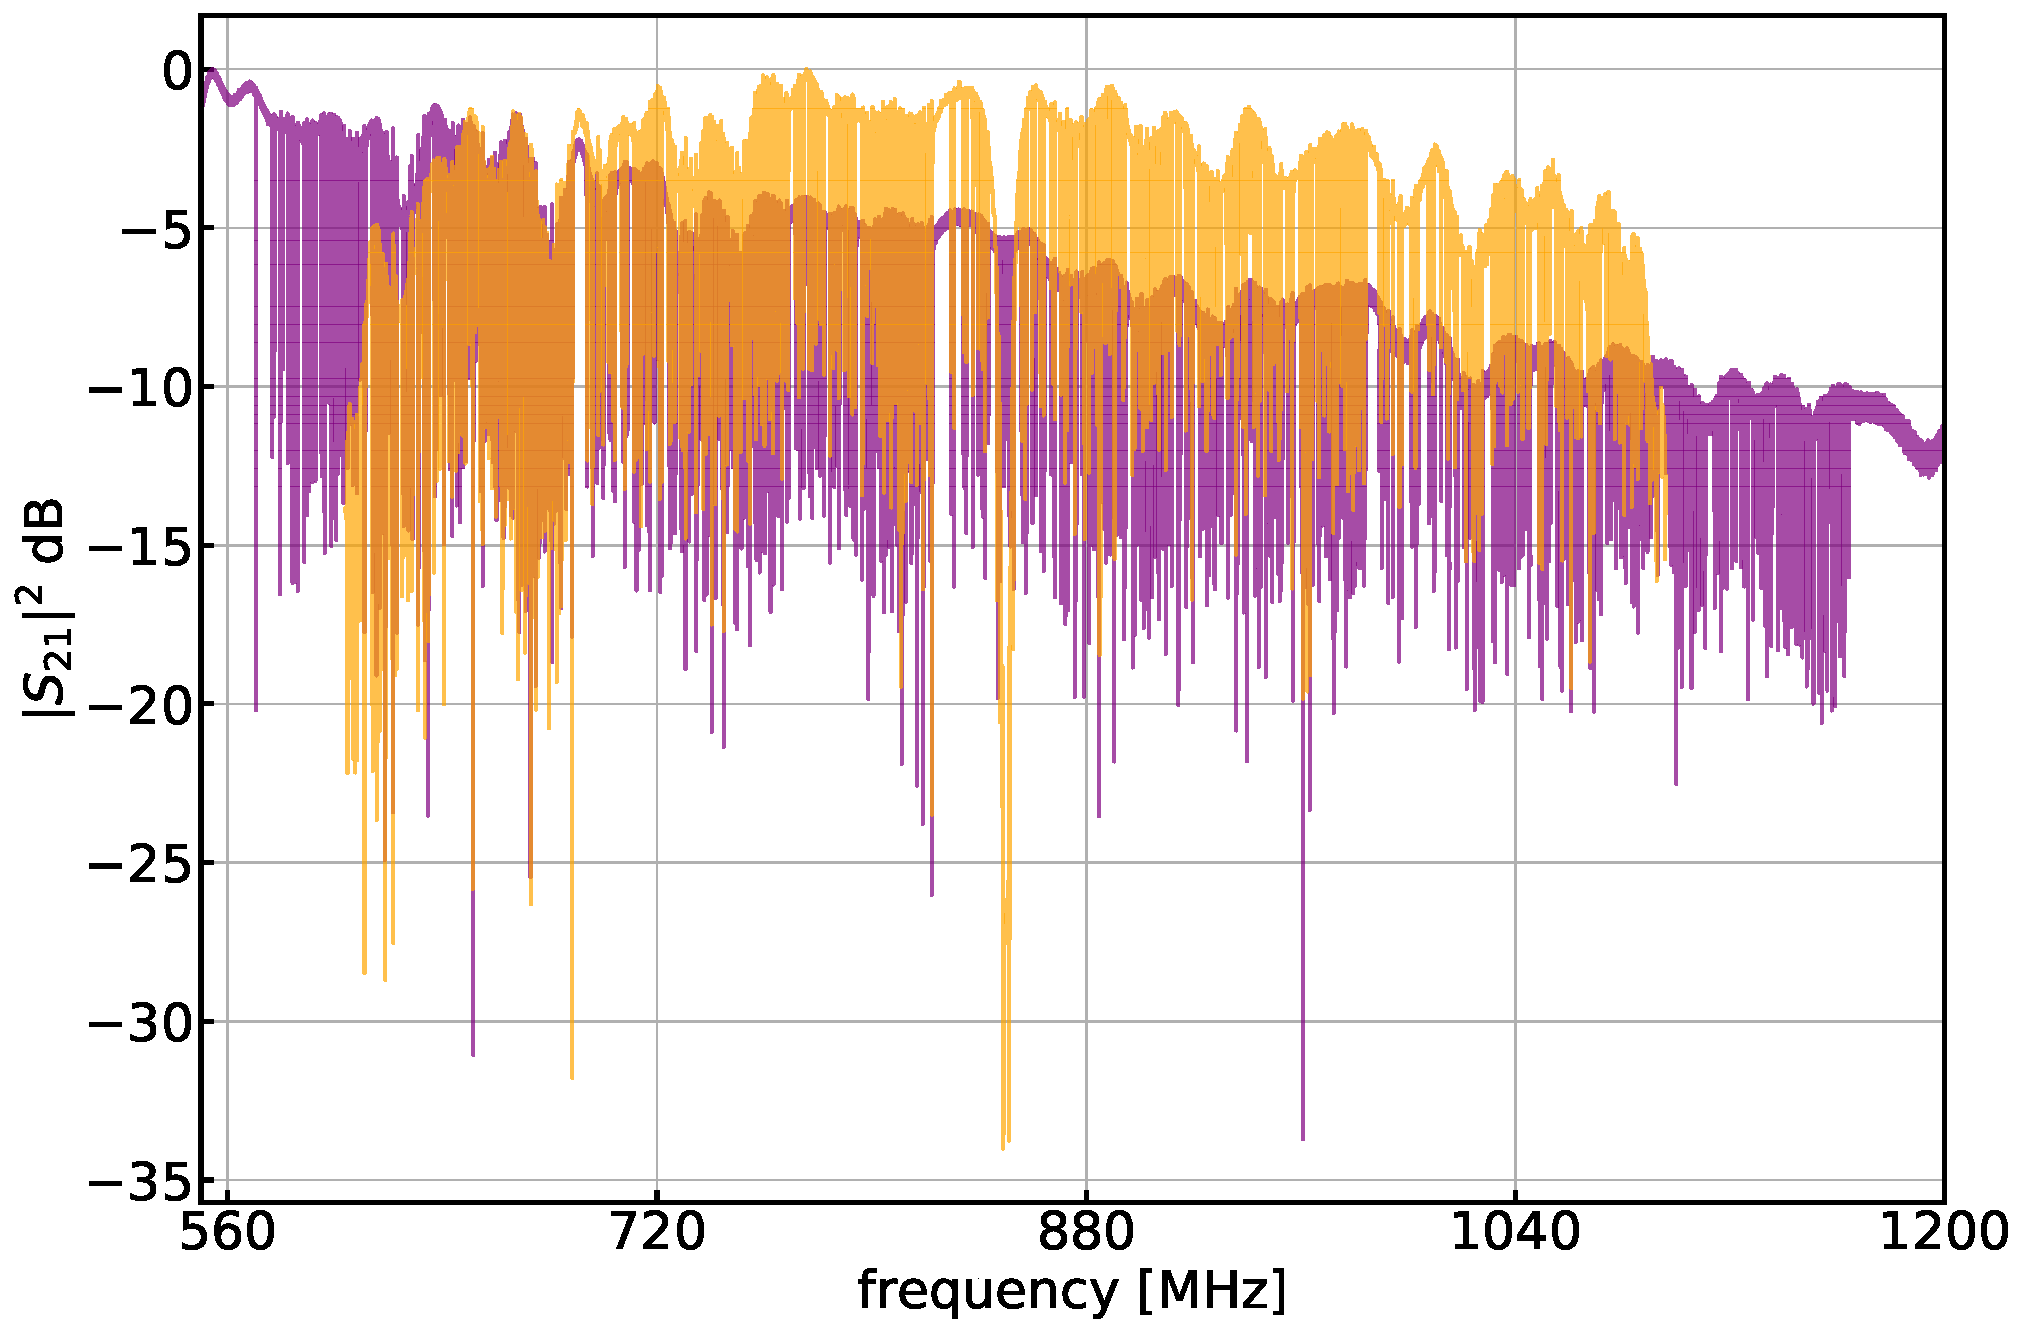
\includegraphics[width=\textwidth]{figures/blast_data/sweeps/350_VNA_overplot}
\caption[~A \macrocapwrap{350~$\upmu$m} ROACH2 sweep from the Palestine integration, with a VNA sweep from May, 2018.]{A 350~$\upmu$m ROACH2 sweep (orange) from the Palestine integration, with a VNA sweep from May, 2018 (purple).}
\label{fig:VNA comp 350}
\end{figure}

\begin{figure}[!htbp]
\centering
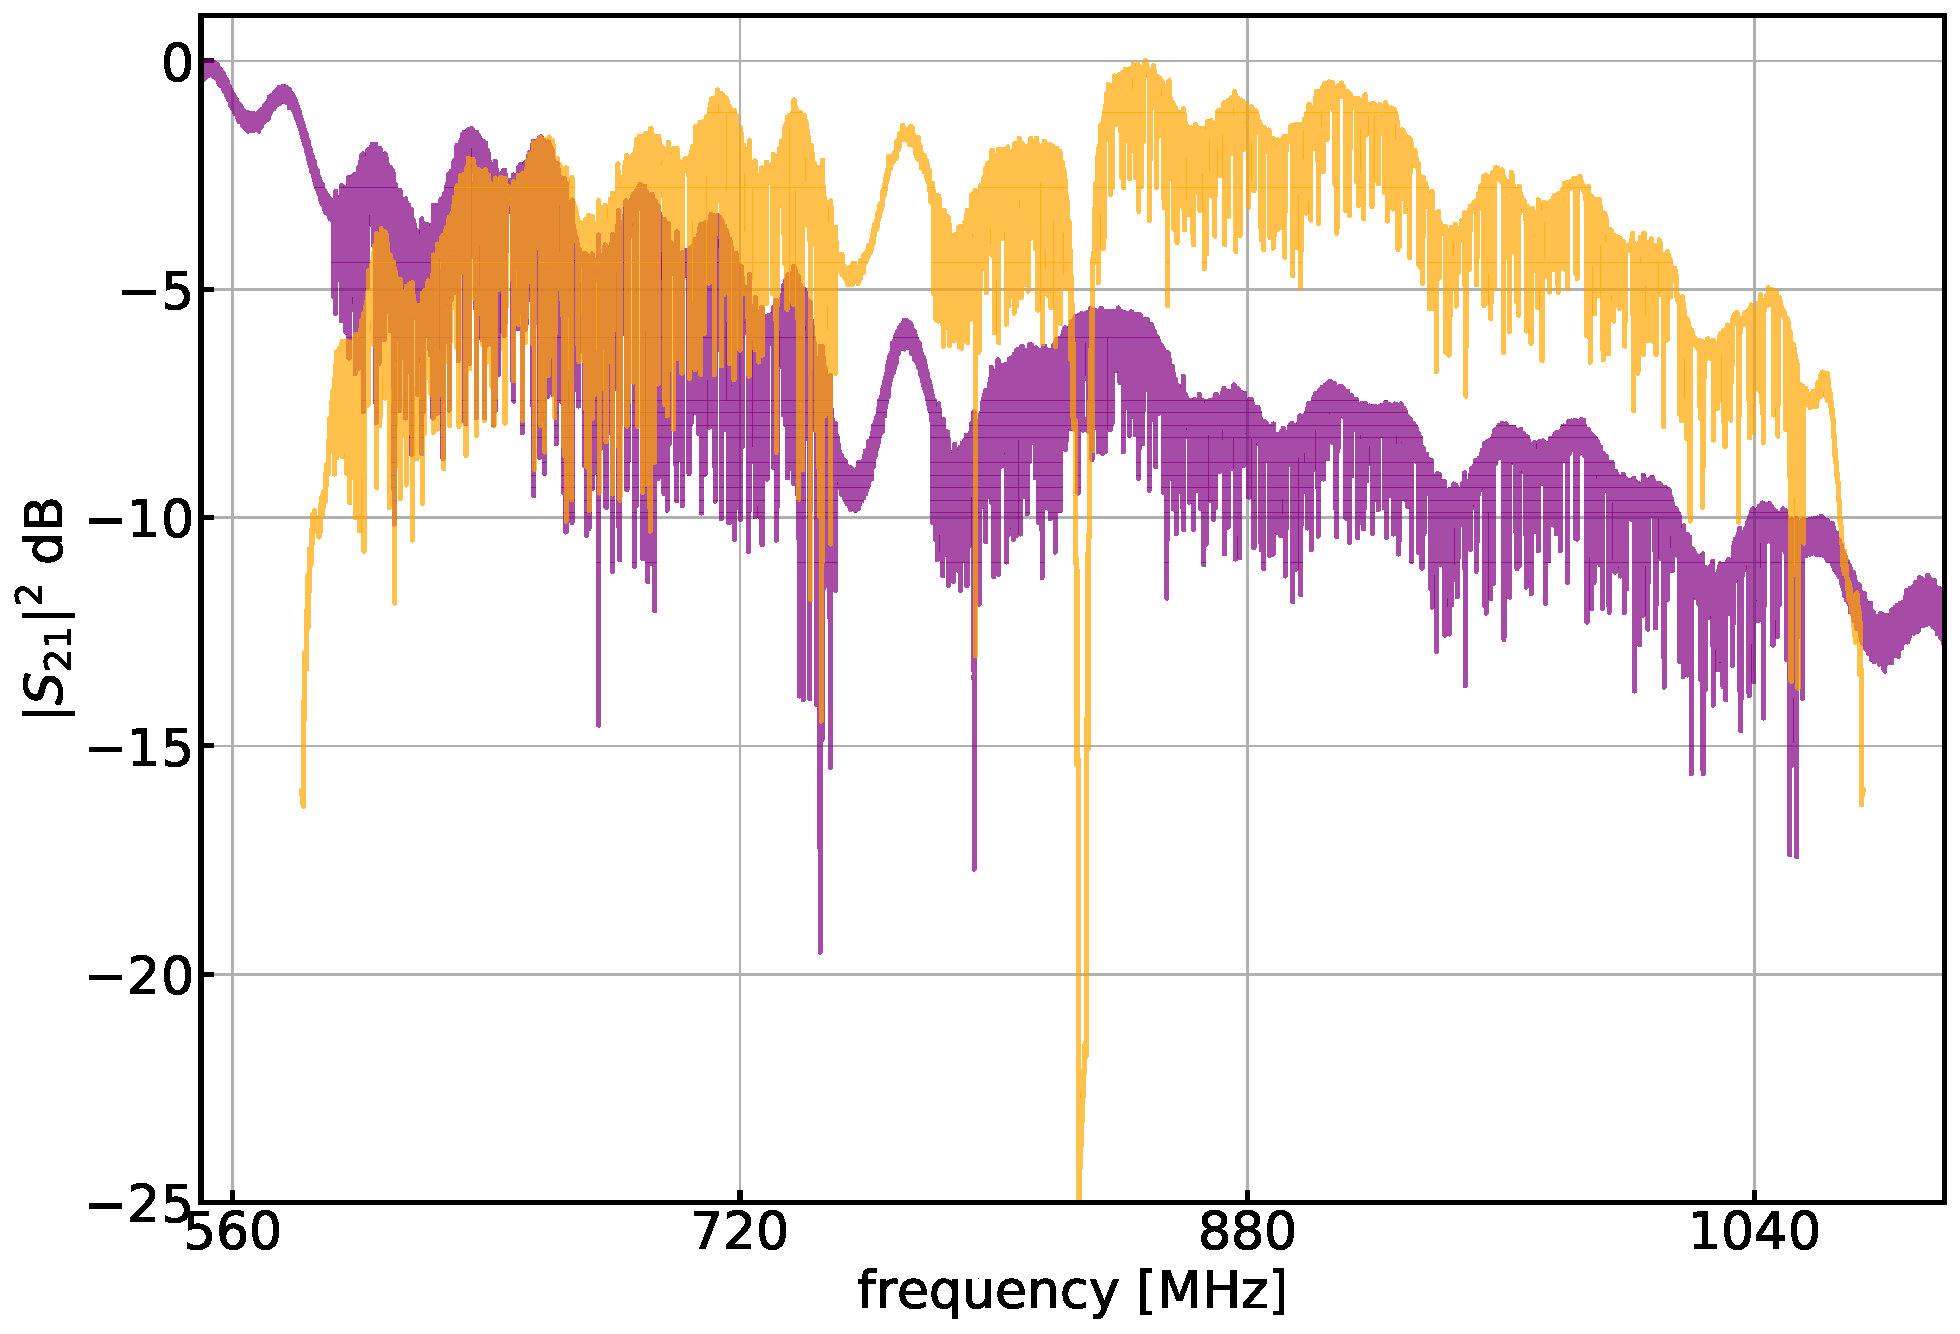
\includegraphics[width=\textwidth]{figures/blast_data/sweeps/250W_VNA_overplot}
\caption[~A 250W ROACH2 sweep from the Palestine integration, with a VNA sweep from May, 2018.]{A 250W ROACH2 sweep (orange) from the Palestine integration, with a VNA sweep from May, 2018 (purple).}
\label{fig:VNA comp 250W}
\end{figure}

\begin{figure}[!htbp]
\centering
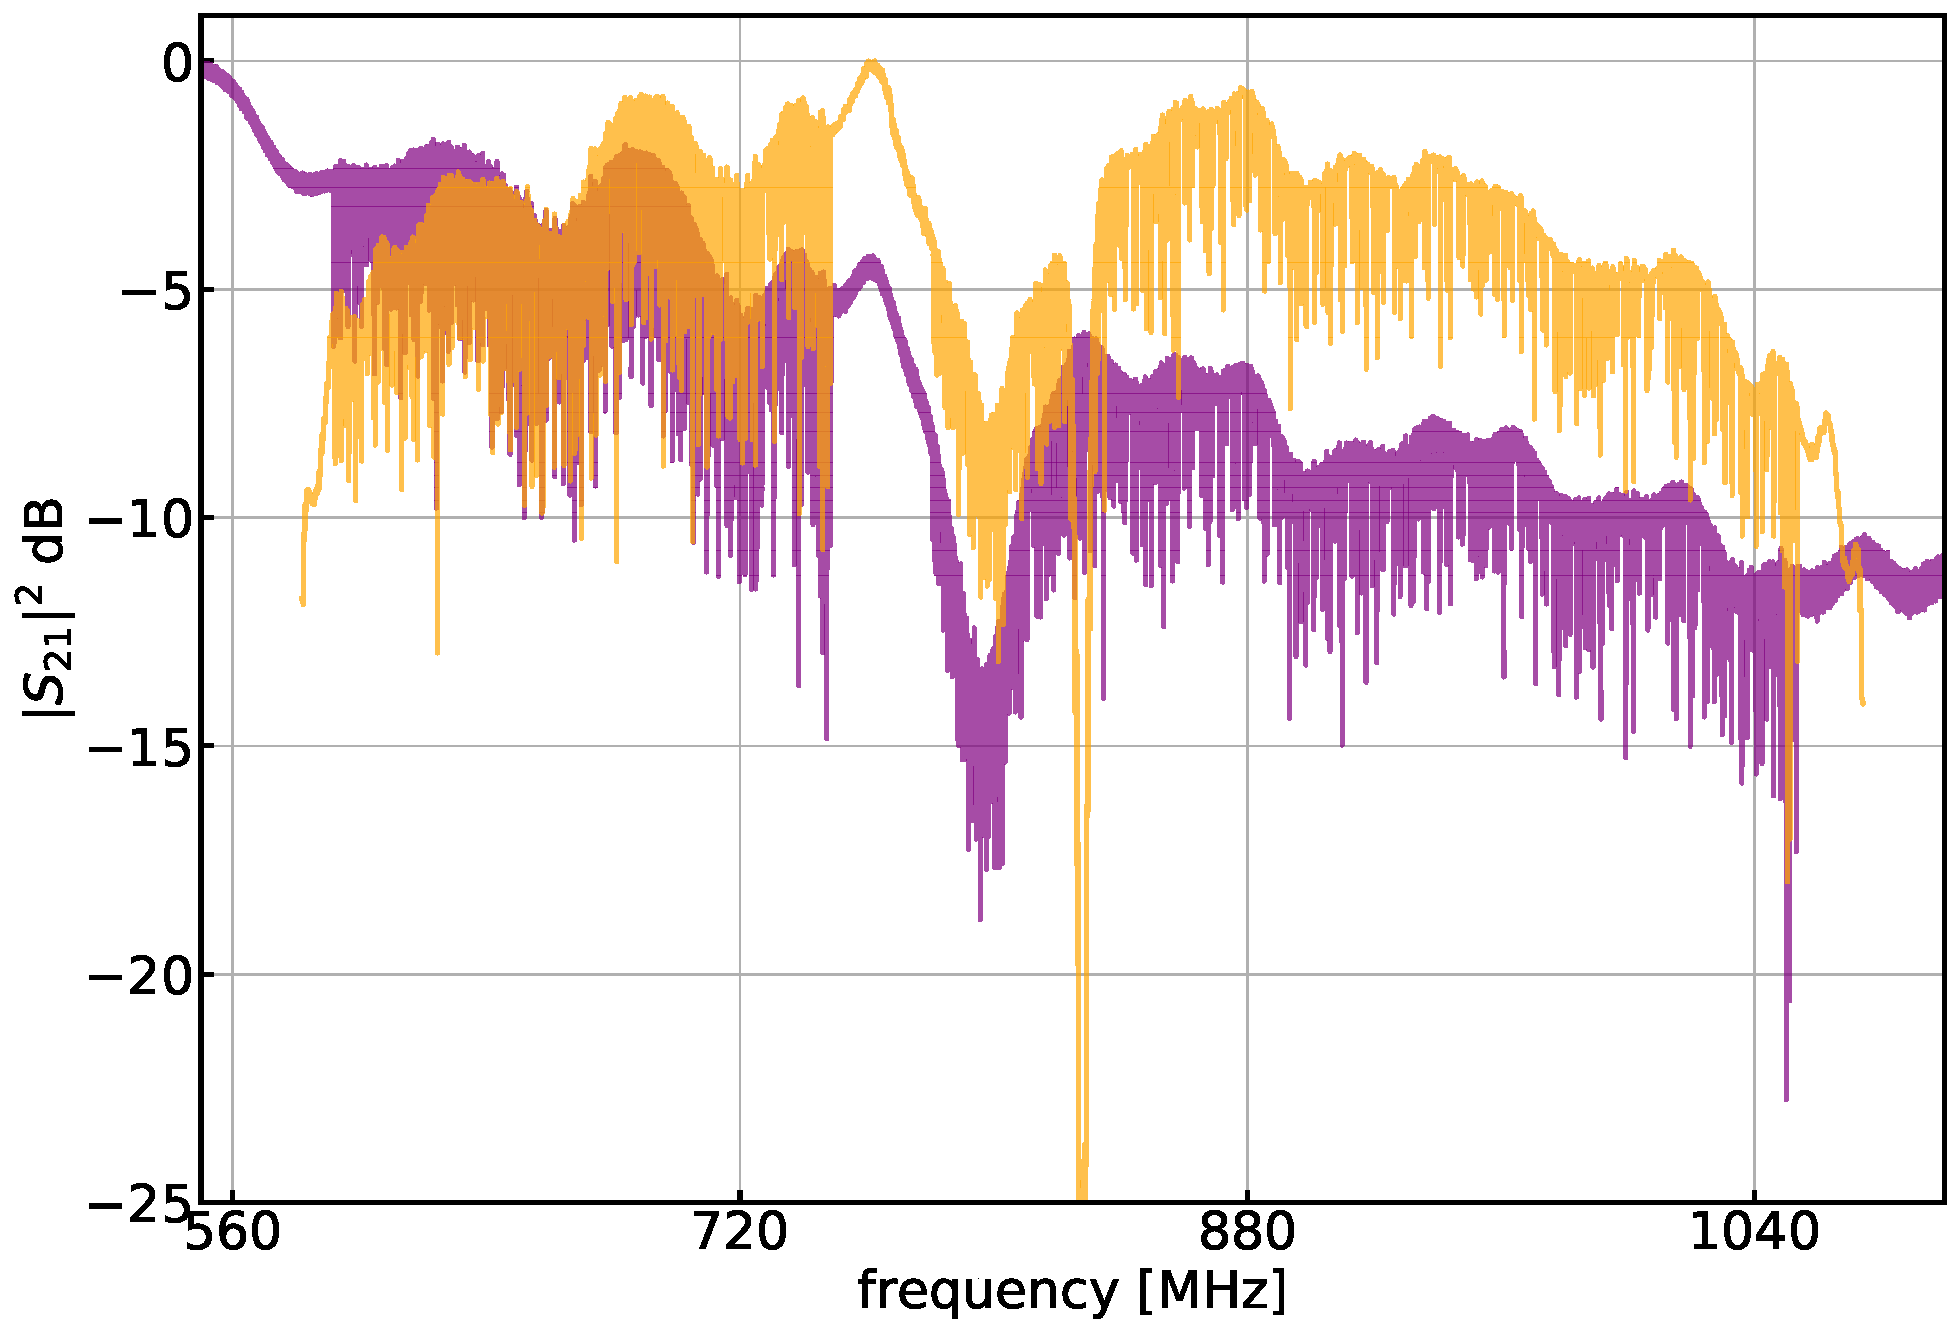
\includegraphics[width=\textwidth]{figures/blast_data/sweeps/250U_VNA_overplot}
\caption[~A 250U ROACH2 sweep from the Palestine integration, with a VNA sweep from May, 2018.]{A 250U ROACH2 sweep (orange) from the Palestine integration, with a VNA sweep from May, 2018 (purple).}
\label{fig:VNA comp 250U}
\end{figure}

\begin{figure}[!htbp]
\centering
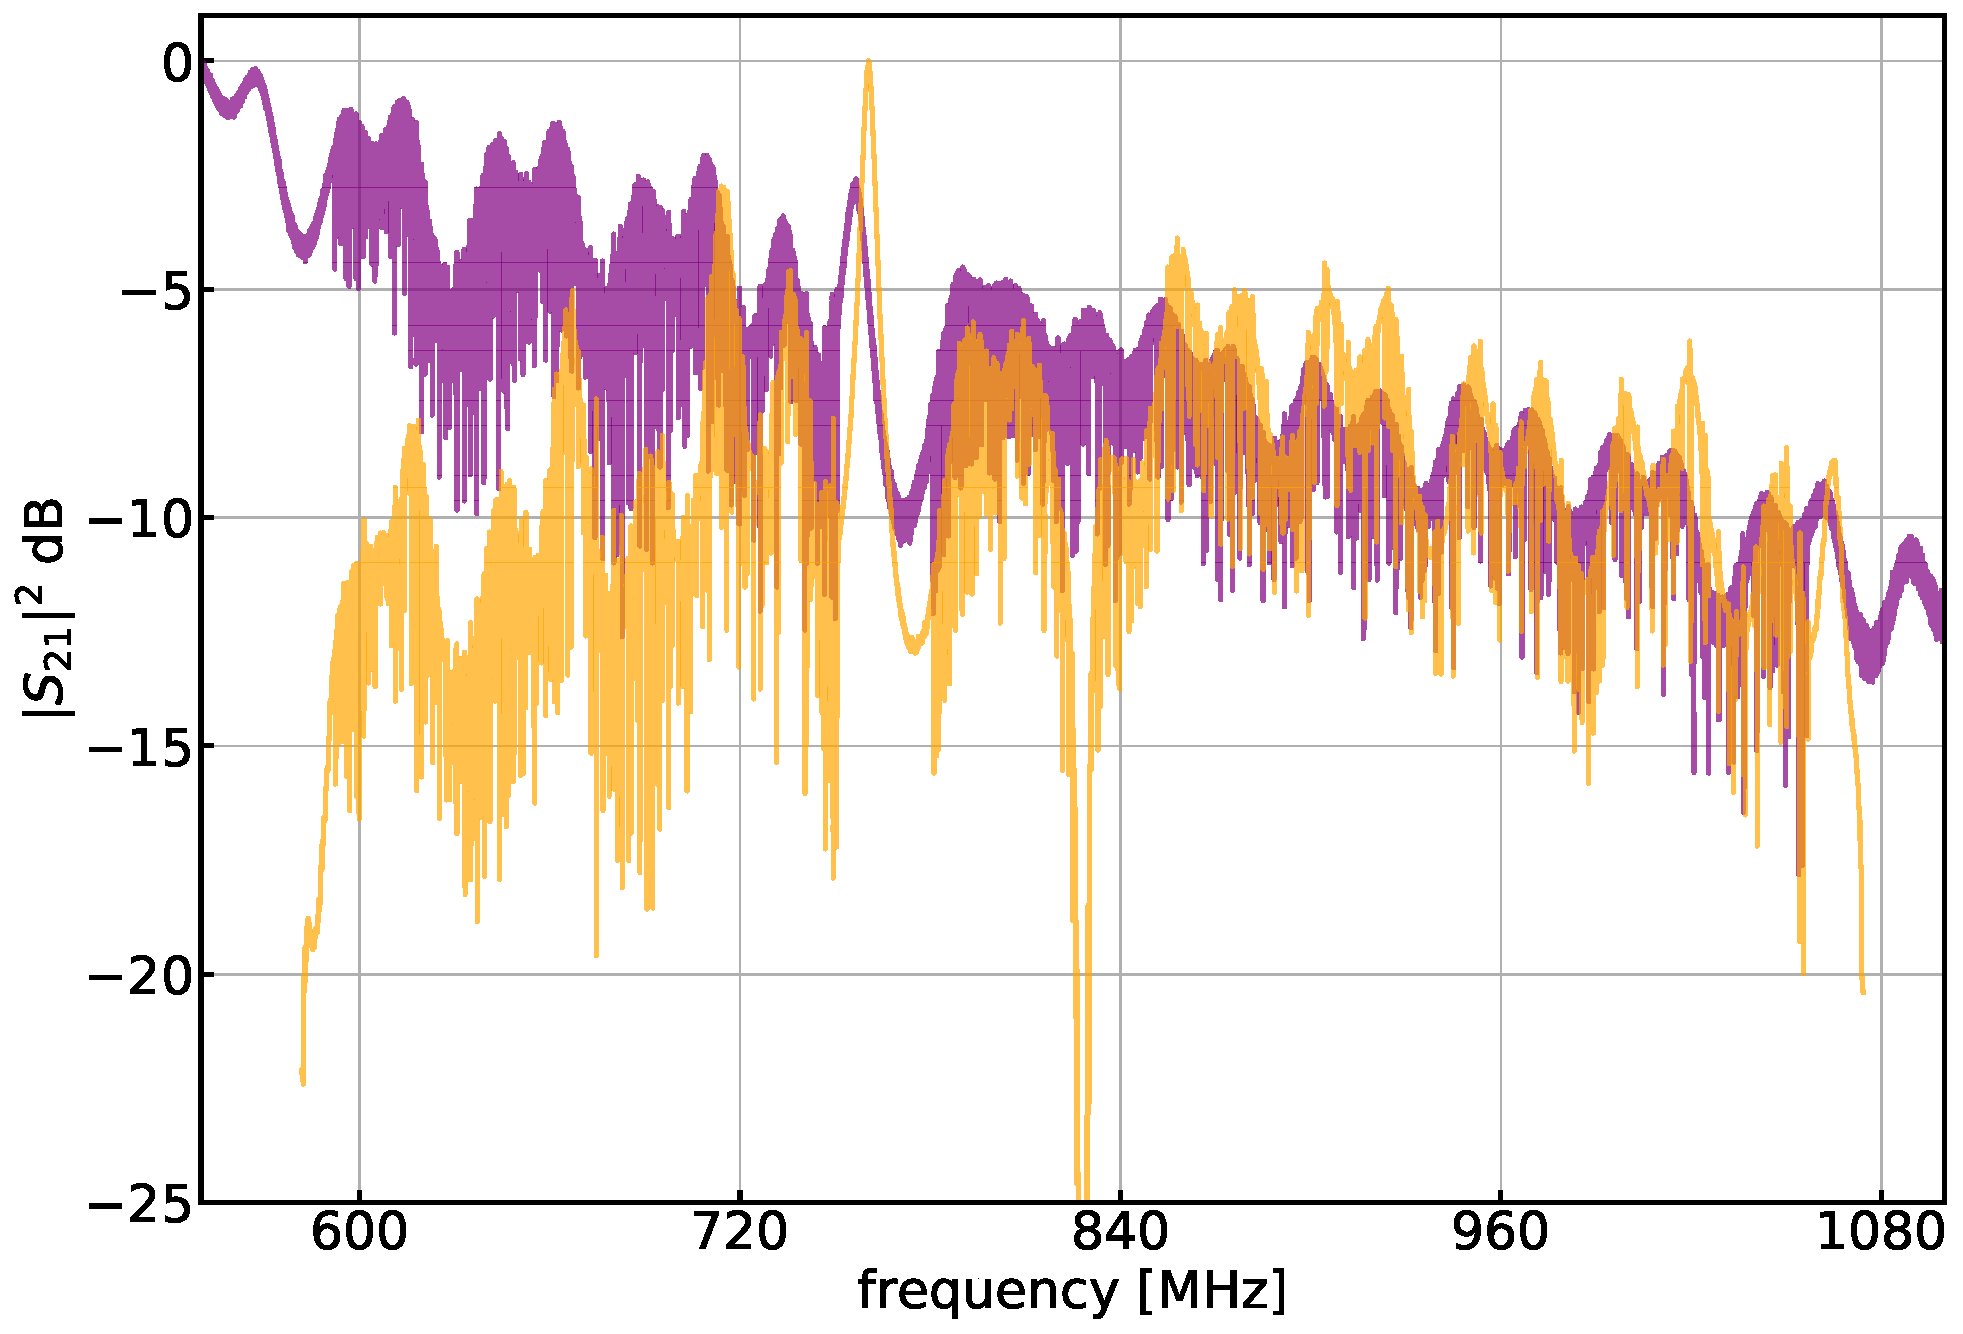
\includegraphics[width=\textwidth]{figures/blast_data/sweeps/250V_VNA_overplot}
\caption[~A 250V ROACH2 sweep from the Palestine integration, with a VNA sweep from May, 2018.]{A 250V ROACH2 sweep (orange) from the Palestine integration, with a VNA sweep from May, 2018 (purple).}
\label{fig:VNA comp 250V}
\end{figure}

\begin{figure}[!htbp]
\centering
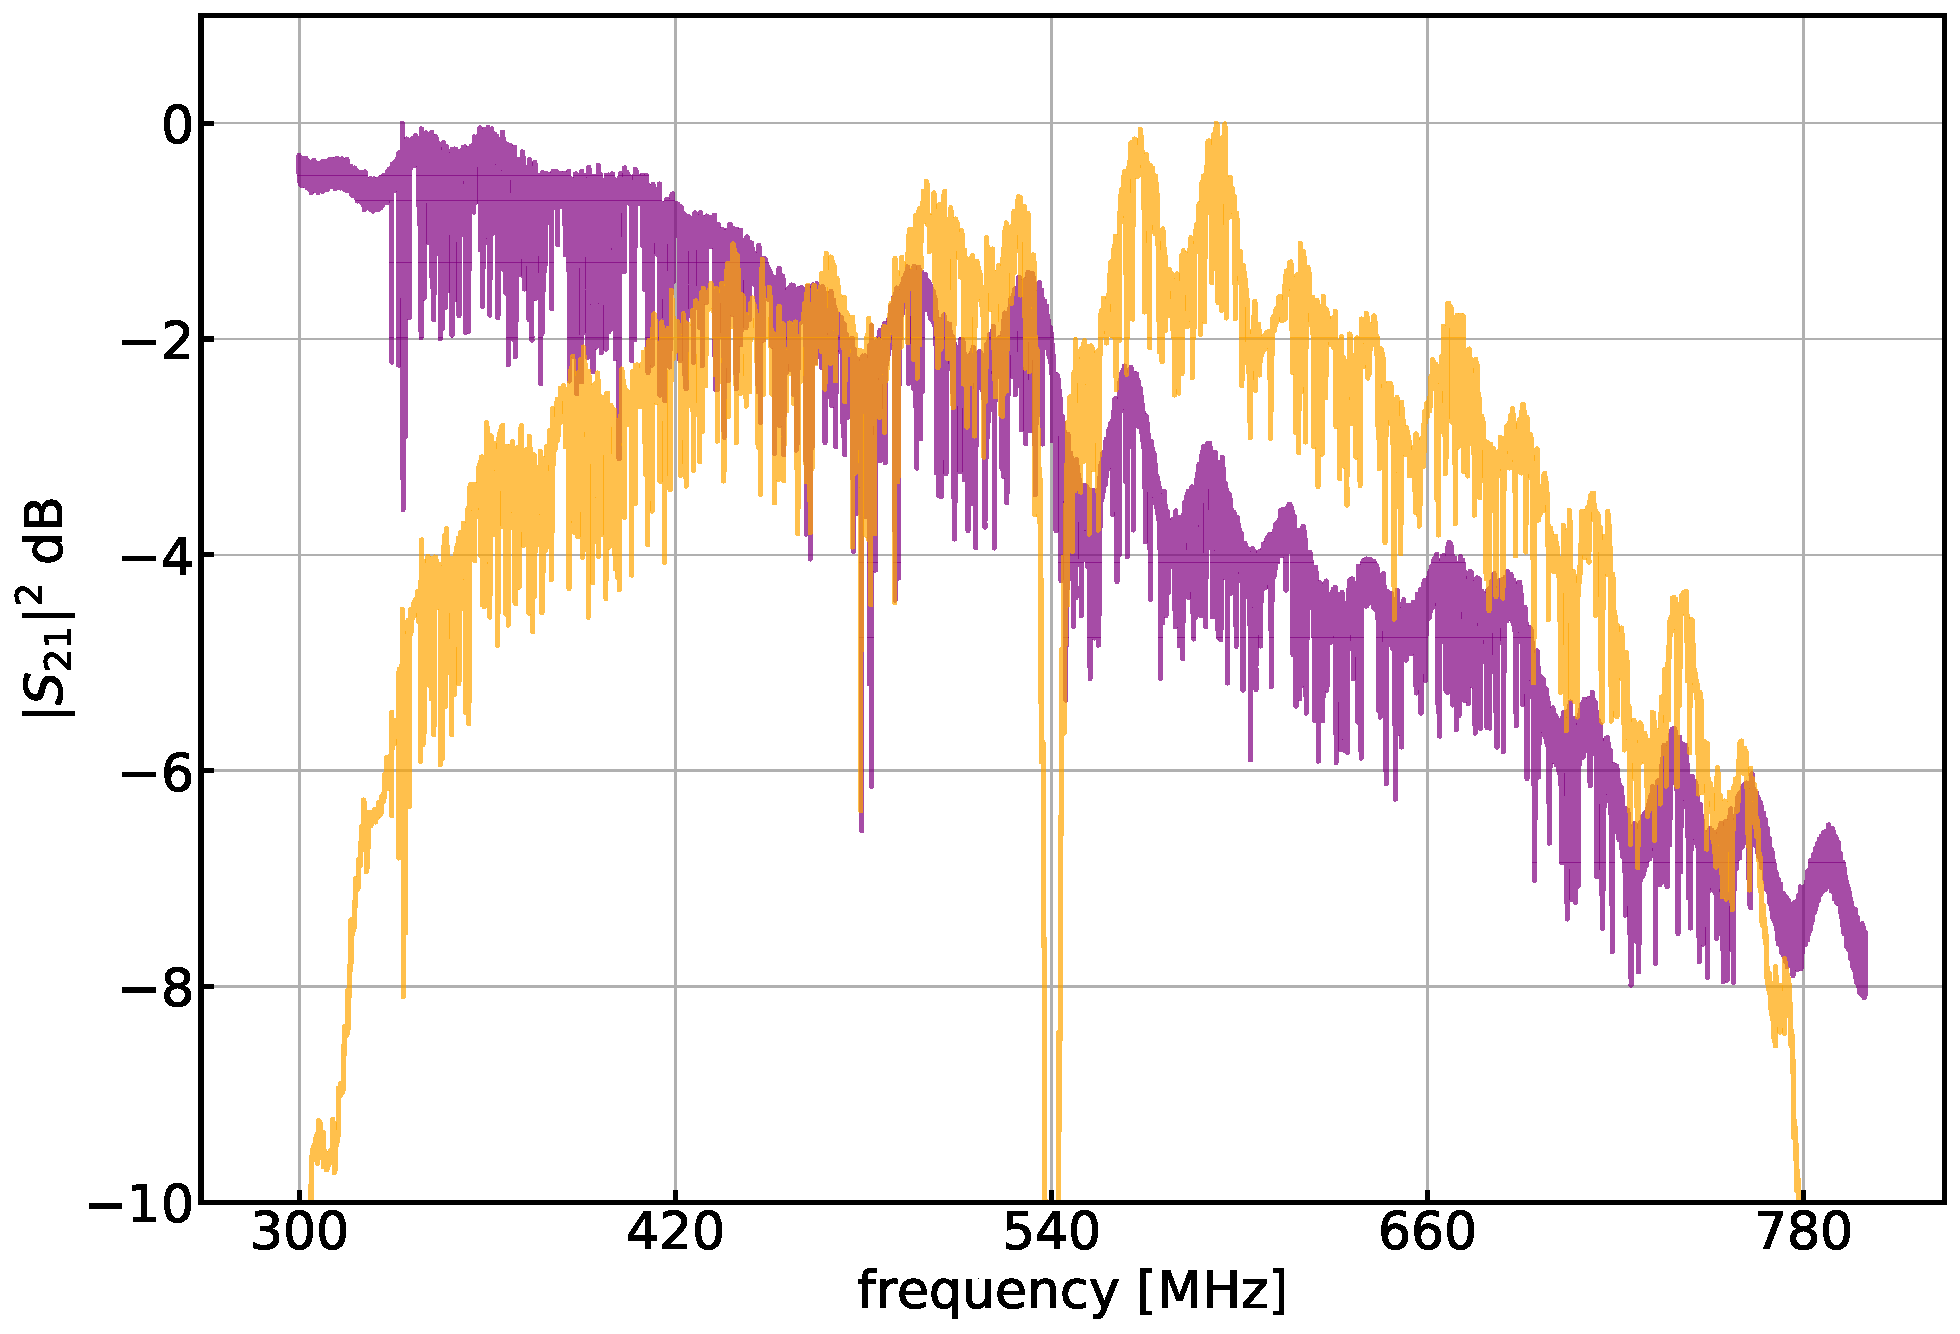
\includegraphics[width=\textwidth]{figures/blast_data/sweeps/500_VNA_overplot}
\caption[~A 500~\macrocapwrap{$\upmu$m} ROACH2 sweep from the Palestine integration, with a VNA sweep from May, 2018.]{A 500~$\upmu$m ROACH2 sweep (orange) from the Palestine integration, with a VNA sweep from May, 2018 (purple).}
\label{fig:VNA comp 500}
\end{figure}

\begin{figure}[!htbp]
\centering
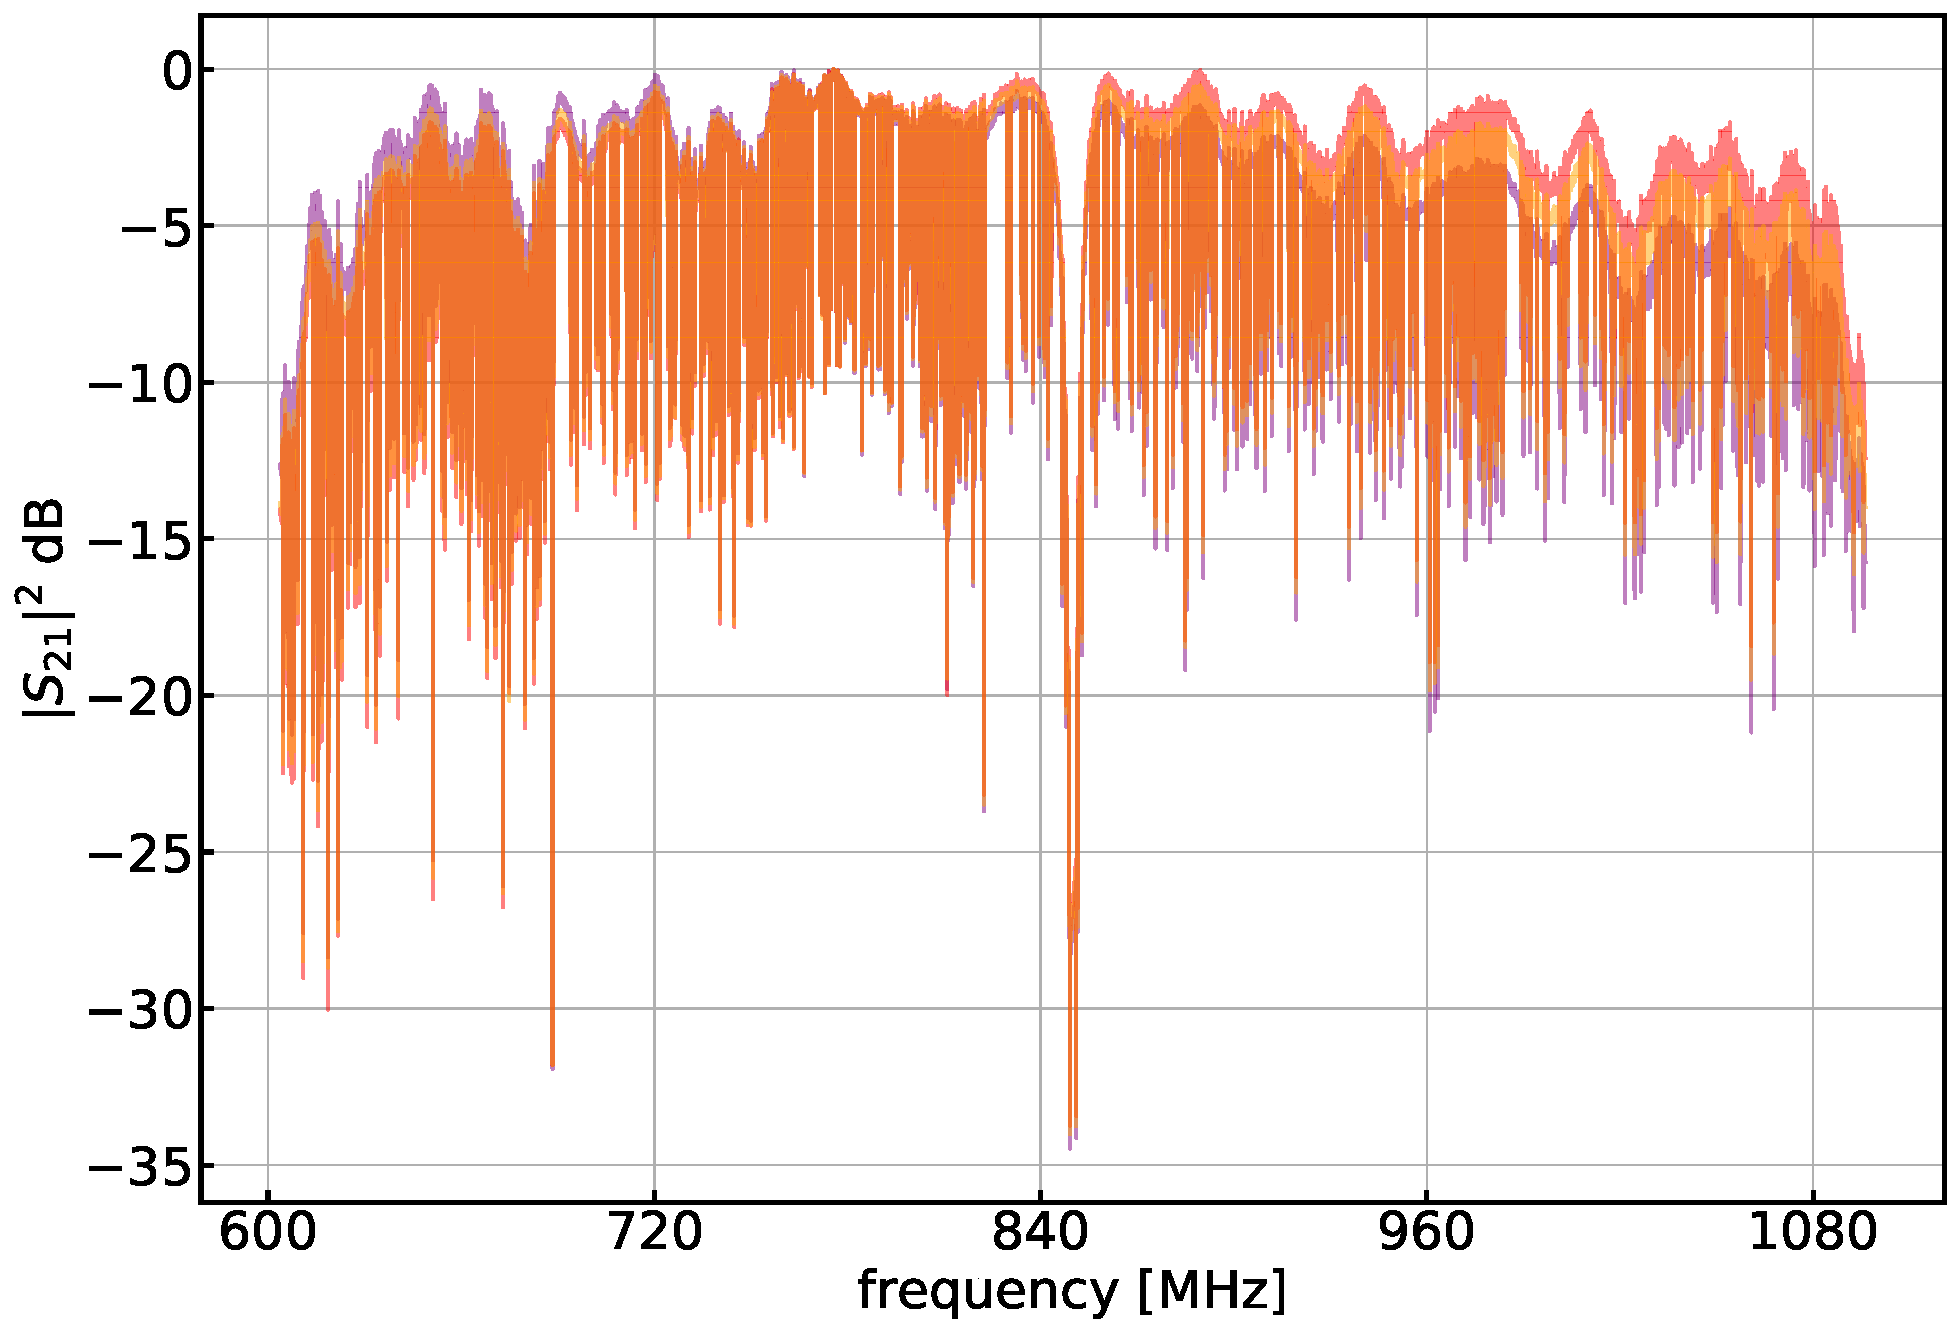
\includegraphics[width=\textwidth]{figures/blast_data/sweeps/trf_slopes}
\caption[~350~\macrocapwrap{$\upmu$m} output transfer function corrections with slopes of 5, 8 and 10~dB.]{350~$\upmu$m output transfer function corrections with 5, 8 and 10~dB slopes accounting for frequency dependent cable loss in the croystat. A VNA trace is shown for comparison.}
\label{fig:trf slopes}
\end{figure}

%%%%%%%%%%%%%%%%%%%%%%%%%%%%%%%%%%%%%%%%%%%%%%%%%%%%%%%%%%%%%%%%%%%%%%%%%%%%%%%
% FIND KIDS
%%%%%%%%%%%%%%%%%%%%%%%%%%%%%%%%%%%%%%%%%%%%%%%%%%%%%%%%%%%%%%%%%%%%%%%%%%%%%%
\subsection{Channel Identification}\label{KID-finding}

The channel frequencies for each array can be determined from a wide ROACH2 sweep (or VNA trace of \gls{S21}). For BLAST-TNG, the steps of the KID-finding algorithm are:

\begin{enumerate}[nosep]
  \item Despike the \gls{S21} trace in linear-space.
  \item Apply a high-pass filter (HPF) to flatten the trace.
  \item Put the trace into log-space, and apply a second HPF\@.
  \item Apply a low-pass filter (LPF) to remove any remaining spurs.
  \item Identify all points in trace below the dip-depth threshold.
  \item Step through points and enforce frequency spacing condition.
  \item Eliminate frequencies in masked regions.
  \item Calculate channel amplitudes from interpolated output TRF\@.
  \item Save channel frequencies and amplitudes to disk.
\end{enumerate}

\vspace{5mm}

\begin{figure}[!htbp]
\centering
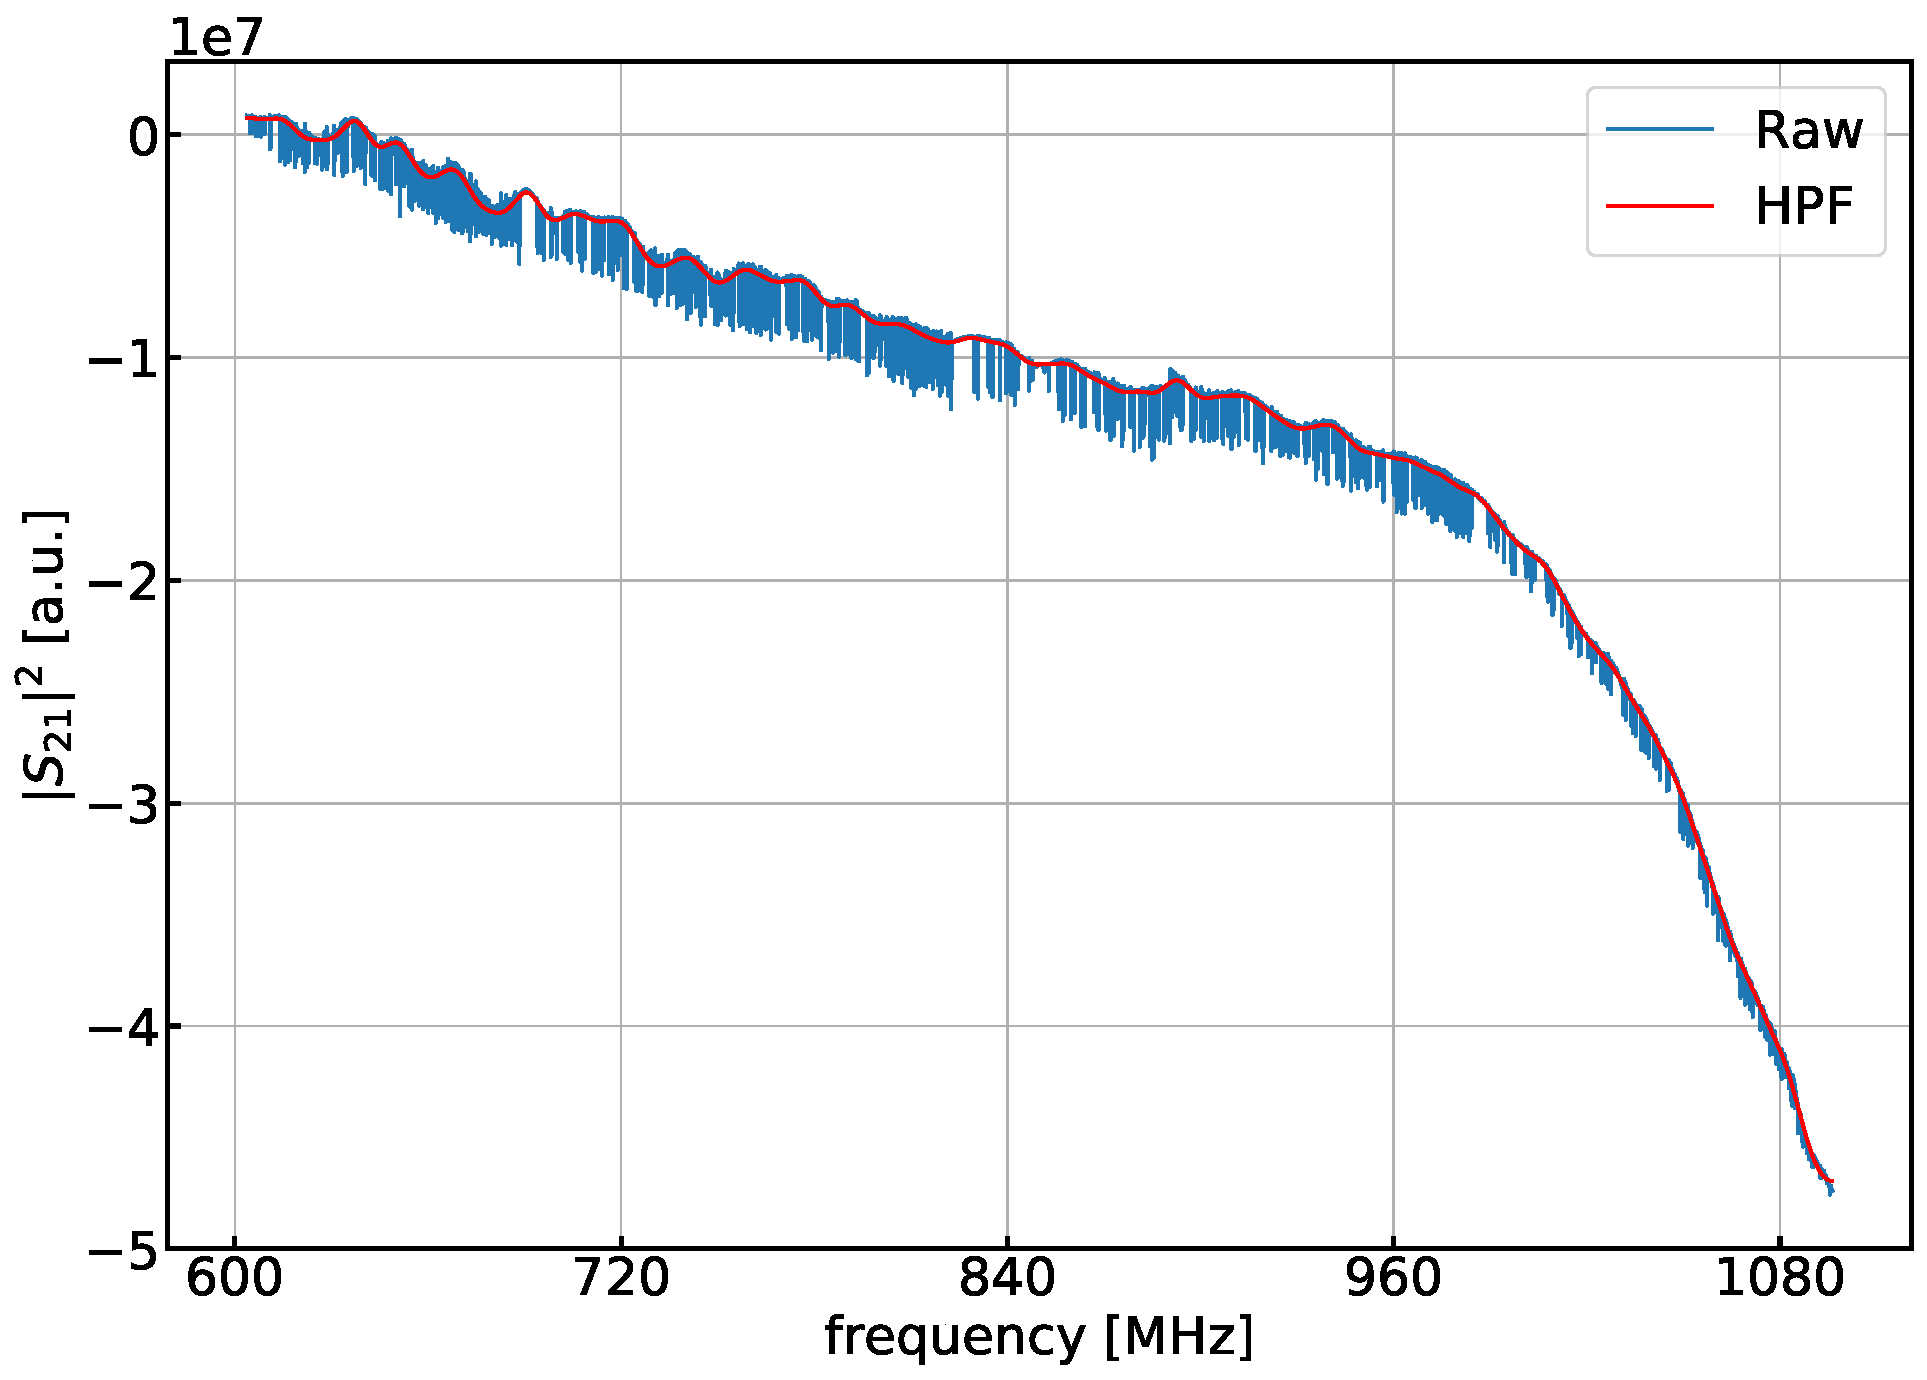
\includegraphics[width=\textwidth]{figures/blast_data/sweeps/350FK_HPF_PAL}
\caption[~The channel alignment and HPF step of the KID-finding algorithm.]{The channel alignment and HPF step of the KID-finding algorithm. The LPF (red) is subtracted from the \gls{S21} trace (blue) prior to frequency identification.}
\label{fig:350FK_HPF}
\end{figure}

This sequence is intended to be performed either at the start of a science observation, or when environmental conditions (fridge temperature drift, optical loading) have shifted the resonators far off of resonance. If the frequency shifts are less than $\sim$2 resonator linewidths, a target sweep may be used to recalibrate the readout frequencies in fewer steps (see Section~\ref{target sweeps}).

The preflight parameters used in the KID-finding process for each BLAST-TNG detector array are listed in Table~\ref{table:KID finding params}. The \gls{S21} sweep is high-pass filtered in (2) and (3) to flatten out the trace envelope as much as possible before identifying points below the dip-depth threshold. The high-pass filtering in (2) is achieved by subtracting a LPF from the data in linear-space. An example of this is shown in Figure~\ref{fig:350FK_HPF}, for the 350~$\upmu$m array. The close spacing of the channels makes it challenging to flatten out the inter-channel frequency space below a level of $\sim$0.1--0.5~dB. Consequently, a small number of `false' channels ($\sim$1--2\% of the total number) are identified by the KID-finding algorithm. The false channels can be manually flagged for removal, or added to the masked regions in (7). The dip-depth threshhold for the 500~$\upmu$m array is set to -0.5 dB due to the intrinsically low \gls{Qr} of the resonators. For the other arrays, the threshold is set to -1 dB.

During channel identification, a frequency spacing threshold of 80--100~kHz is enforced. If two channels are spaced by less than this threshold, the channel with the shallow dip-depth is omitted from the final frequency list. The masked regions listed in Table~\ref{table:KID finding params} are ignored during the KID-finding process. These regions include a 10~MHz window above and below the center of the band (f$_\mathrm{LO}$), and narrow bands which sometimes contain spurious noise thought to be associated with RF interference (RFI).

\subsection{Detector Yields}\label{yields}

\begin{table}[!hbtp]
  \centering
  \begin{threeparttable}
    \caption{Parameters used in KID-finding process for each BLAST-TNG detector array.}
\begin{tabular}{@{}llllll@{}}
\dtoprule{}
 & 250U~$\upmu$m & 250V~$\upmu$m & 250W~$\upmu$m & 350~$\upmu$m & 500~$\upmu$m \\ \midrule
LPF f$_{c}$ (MHz) & 10 & 5 & 5 & 10 & 10 \\
Dip-depth thresh. (dB) & -1 & -1 & -1 & -1 & -0.5 \\
Spacing thresh. (kHz) & 100 & 100 & 100 & 100 & 100 \\
f$_\mathrm{LO}$ (MHz)\tnote{1} & 827 & 829 & 828 & 850 & 540 \\
f$_{\mathrm{low-cut}}$ (MHz) & 590 & 590 & 590 & 604.5 & 326 \\
f$_{\mathrm{high-cut}}$ (MHz) & 1060 & 1060 & 1060 & 1089 & 762 \\
f$_{\mathrm{mask,low}}$ (MHz)\tnote{2} &  & 820 & 751, 818 & 845 & 450.8, 535 \\
f$_{\mathrm{mask,high}}$ (MHz)\tnote{3} &  & 835 & 770, 838 & 855 & 451.8, 545 \\ \dbottomrule{}
\\
\end{tabular}
\begin{tablenotes}
\item [1] The LO center-frequency.
\item [2] The start frequencies of masked regions.
\item [3] The stop frequencies of masked regions.
\vspace{2mm}
\end{tablenotes}
\label{table:KID finding params}
\end{threeparttable}
\end{table}

Detector yields for each BLAST-TNG array determined using the ROACH2 readout during the Palestine and Antarctica integrations are listed in Table~\ref{table:det yields}. In the table, N$_{\mathrm{design}}$ refers to the number of channels on each array which were reported by NIST\@. With the exception of the 350~$\upmu$m array, this value is not necessarily the actual number of channels within the 512~MHz ROACH2 readout bandwidth. As a baseline channel count, we adopt the number of channels which were found by applying the KID-finding algorithm to dark VNA \gls{S21} sweeps taken during May, 2018 (N$_{\mathrm{May18,VNA}}$). The yields are then calculated by comparing the channel counts found during the Palestine and Antarctica integrations to N$_{\mathrm{May18,VNA}}$. The Palestine yields (Y$_{\mathrm{PAL/VNA}}$) are around 85\% for each array. During the Palestine integration, a $\sim$4\% neutral-density filter (NDF) was installed in the array. The NDF was not present during the Antarctica integration, and the increased optical loading on the arrays made it challenging to identify all of the channels (particularly in the case of the 500~$\upmu$m array). The 250V array was not used during ice testing due to a damaged component in the cold RF-chain.

\begin{table}[!htbp]
  \centering
  \begin{threeparttable}
    \caption[~Detector yields for each BLAST-TNG detector array.]{Detector yields for each BLAST-TNG detector array.}
\begin{tabular}{@{}llllll@{}}
\dtoprule{}
                        & 250U       & 250V \tnote{1} & 250W    &350~$\upmu$m       & 500~$\upmu$m \\ \midrule
N$_{\mathrm{design}}$\tnote{3}   & 612        & 612         & 612        & 775\tnote{2}     & 468     \\
N$_{\mathrm{May18,VNA}}$\tnote{4}& 500        & 521         & 495        & 683              & 381     \\
N$_{\mathrm{PAL}}$ \tnote{5}     & 390        & 237         & 412        & 626              & 326     \\
N$_{\mathrm{ICE}}$ \tnote{6}     & 508        &             & 466        & 619              & 260     \\
Y$_{\mathrm{VNA/design}}$\tnote{7} & 0.82     & 0.85        & 0.81       & 0.88             & 0.81    \\
Y$_{\mathrm{PAL/VNA}}$           & 0.78       & 0.45        & 0.83       & 0.92             & 0.86    \\
Y$_{\mathrm{ICE/VNA}}$           & 1.01       &             & 0.94       & 0.91             & 0.68    \\ \dbottomrule{}
\\
\end{tabular}
\begin{tablenotes}
\item [1] The 250V cold RF chain was damaged on the ice, and the array was not used during testing.
\item [2] Number of detectors within the readout band of 512 MHz.
\item [3] Number of detectors on each array, reported by NIST\@.
\item [4] Number of detectors identified in a May, 2018 VNA sweep.
\item [5] Number of detectors identified in ROACH sweeps during Palestine integration.
\item [6] Number of detectors identified in ROACH sweeps during preflight ice integration.
\vspace{2mm}
\end{tablenotes}
\label{table:det yields}
\end{threeparttable}
\end{table}

Figures~\ref{fig:350 VNA FK} to~\ref{fig:500 VNA FK} show the results of the KID-finding algorithm applied to the VNA, Palestine and Antarctica sweeps of each array. Selected channels are marked with red stars. The dip-depth threshold is shown as a dashed red line, and masked regions are highlighted in green.

% VNA overplot
\begin{figure}[!p]
\centering
\caption[~\macrocapwrap{350~$\upmu$m} array KID-finding results.]{350~$\upmu$m array KID-finding results for a VNA sweep (top) and ROACH2 sweeps from Palestine (middle) and the ice (bottom).}
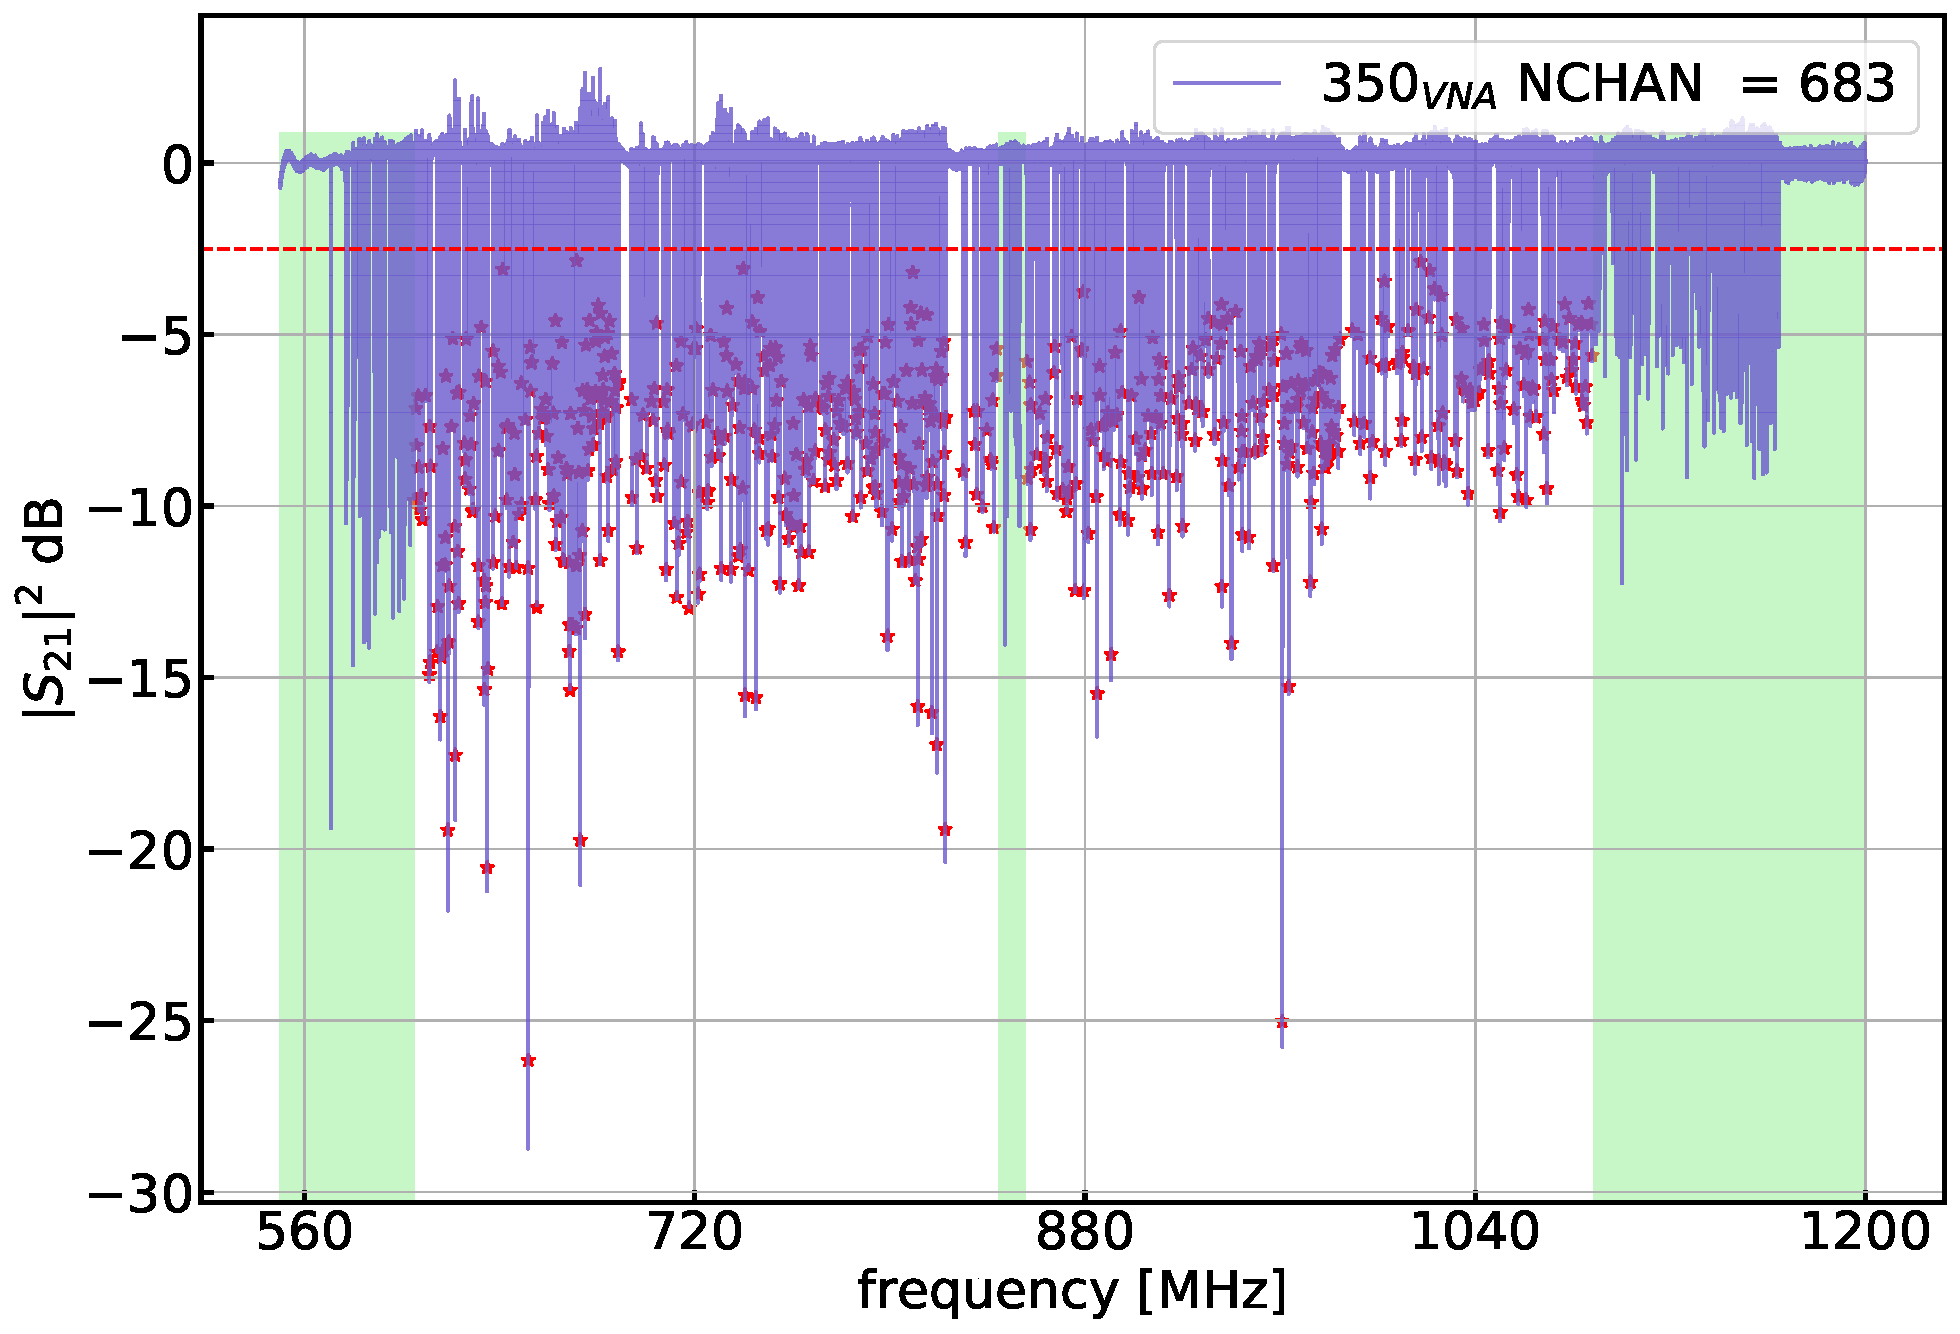
\includegraphics[width=0.68\textwidth]{figures/blast_data/sweeps/350_May2018VNA_FK}
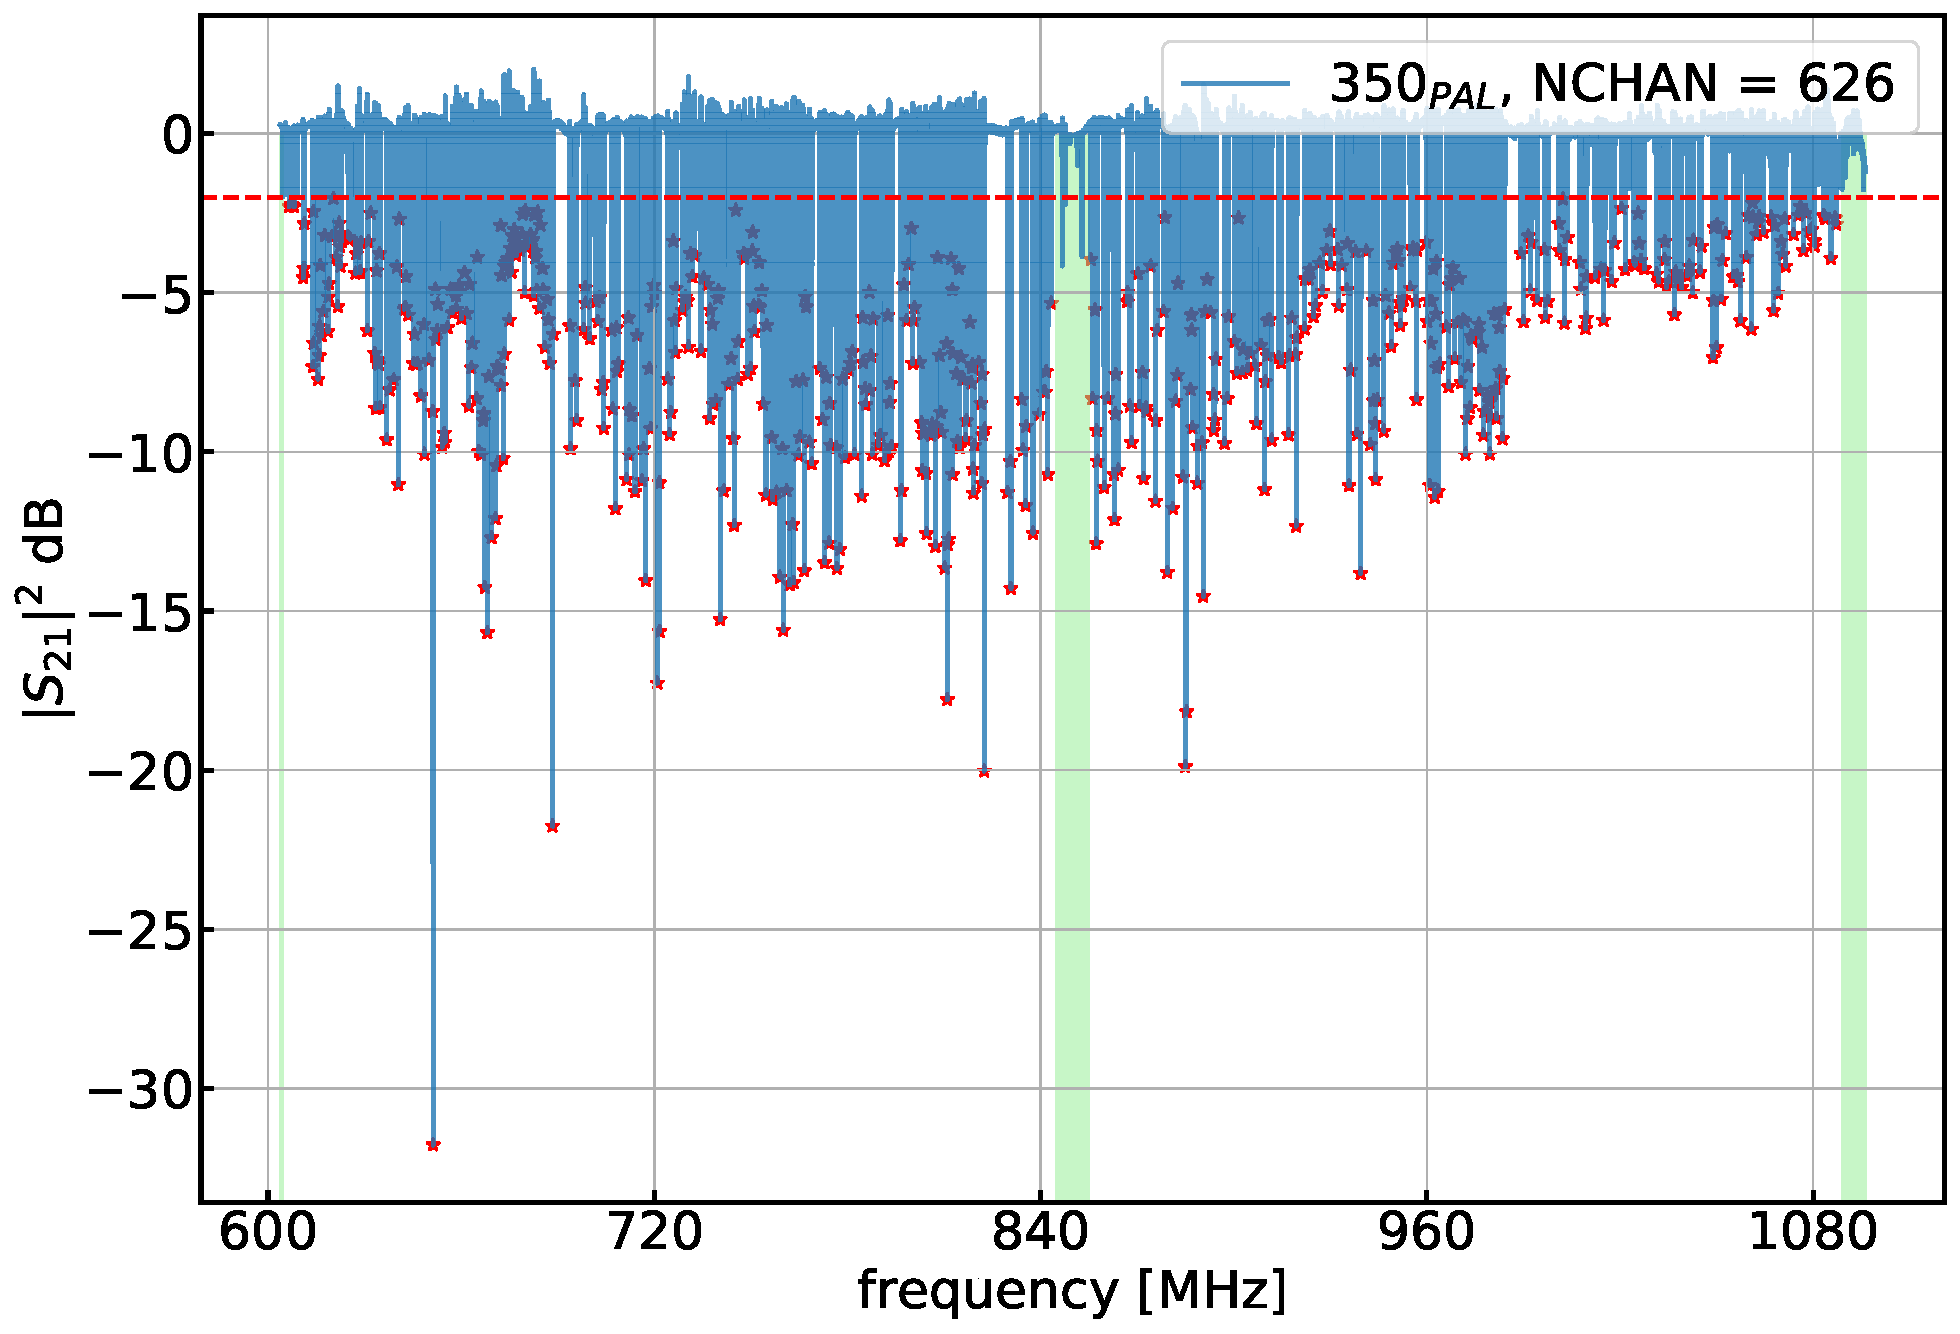
\includegraphics[width=0.68\textwidth]{figures/blast_data/sweeps/350_PAL_FK}
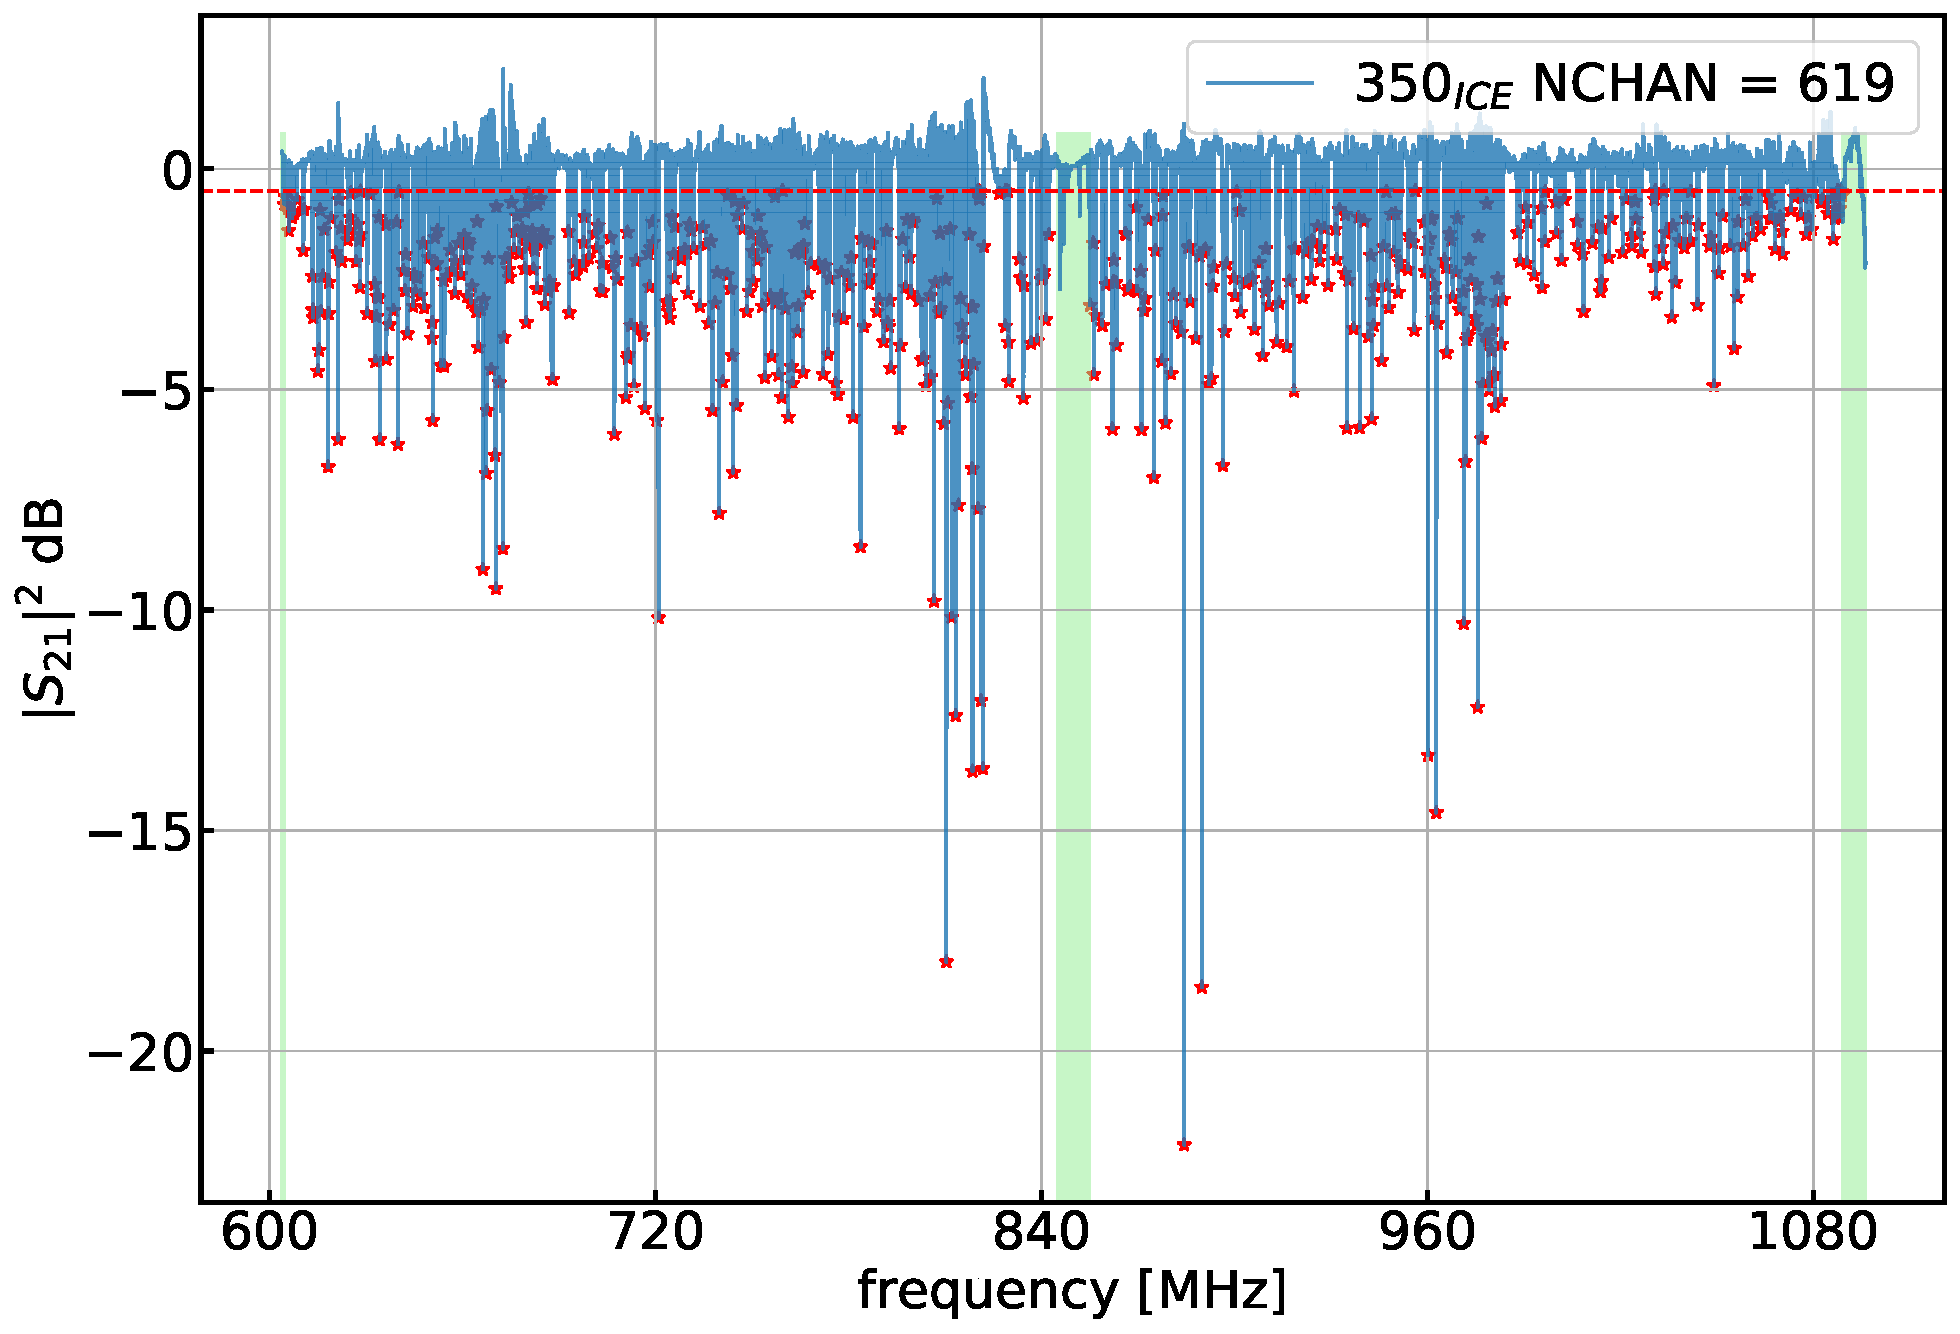
\includegraphics[width=0.68\textwidth]{figures/blast_data/sweeps/350_ICE_FK}
\label{fig:350 VNA FK}
\end{figure}

% 250 W

\begin{figure}[!p]
\centering
\caption[~250W array KID-finding results.]{250W array KID-finding results for a VNA sweep (top) and ROACH2 sweeps from Palestine (middle) and the ice (bottom).}
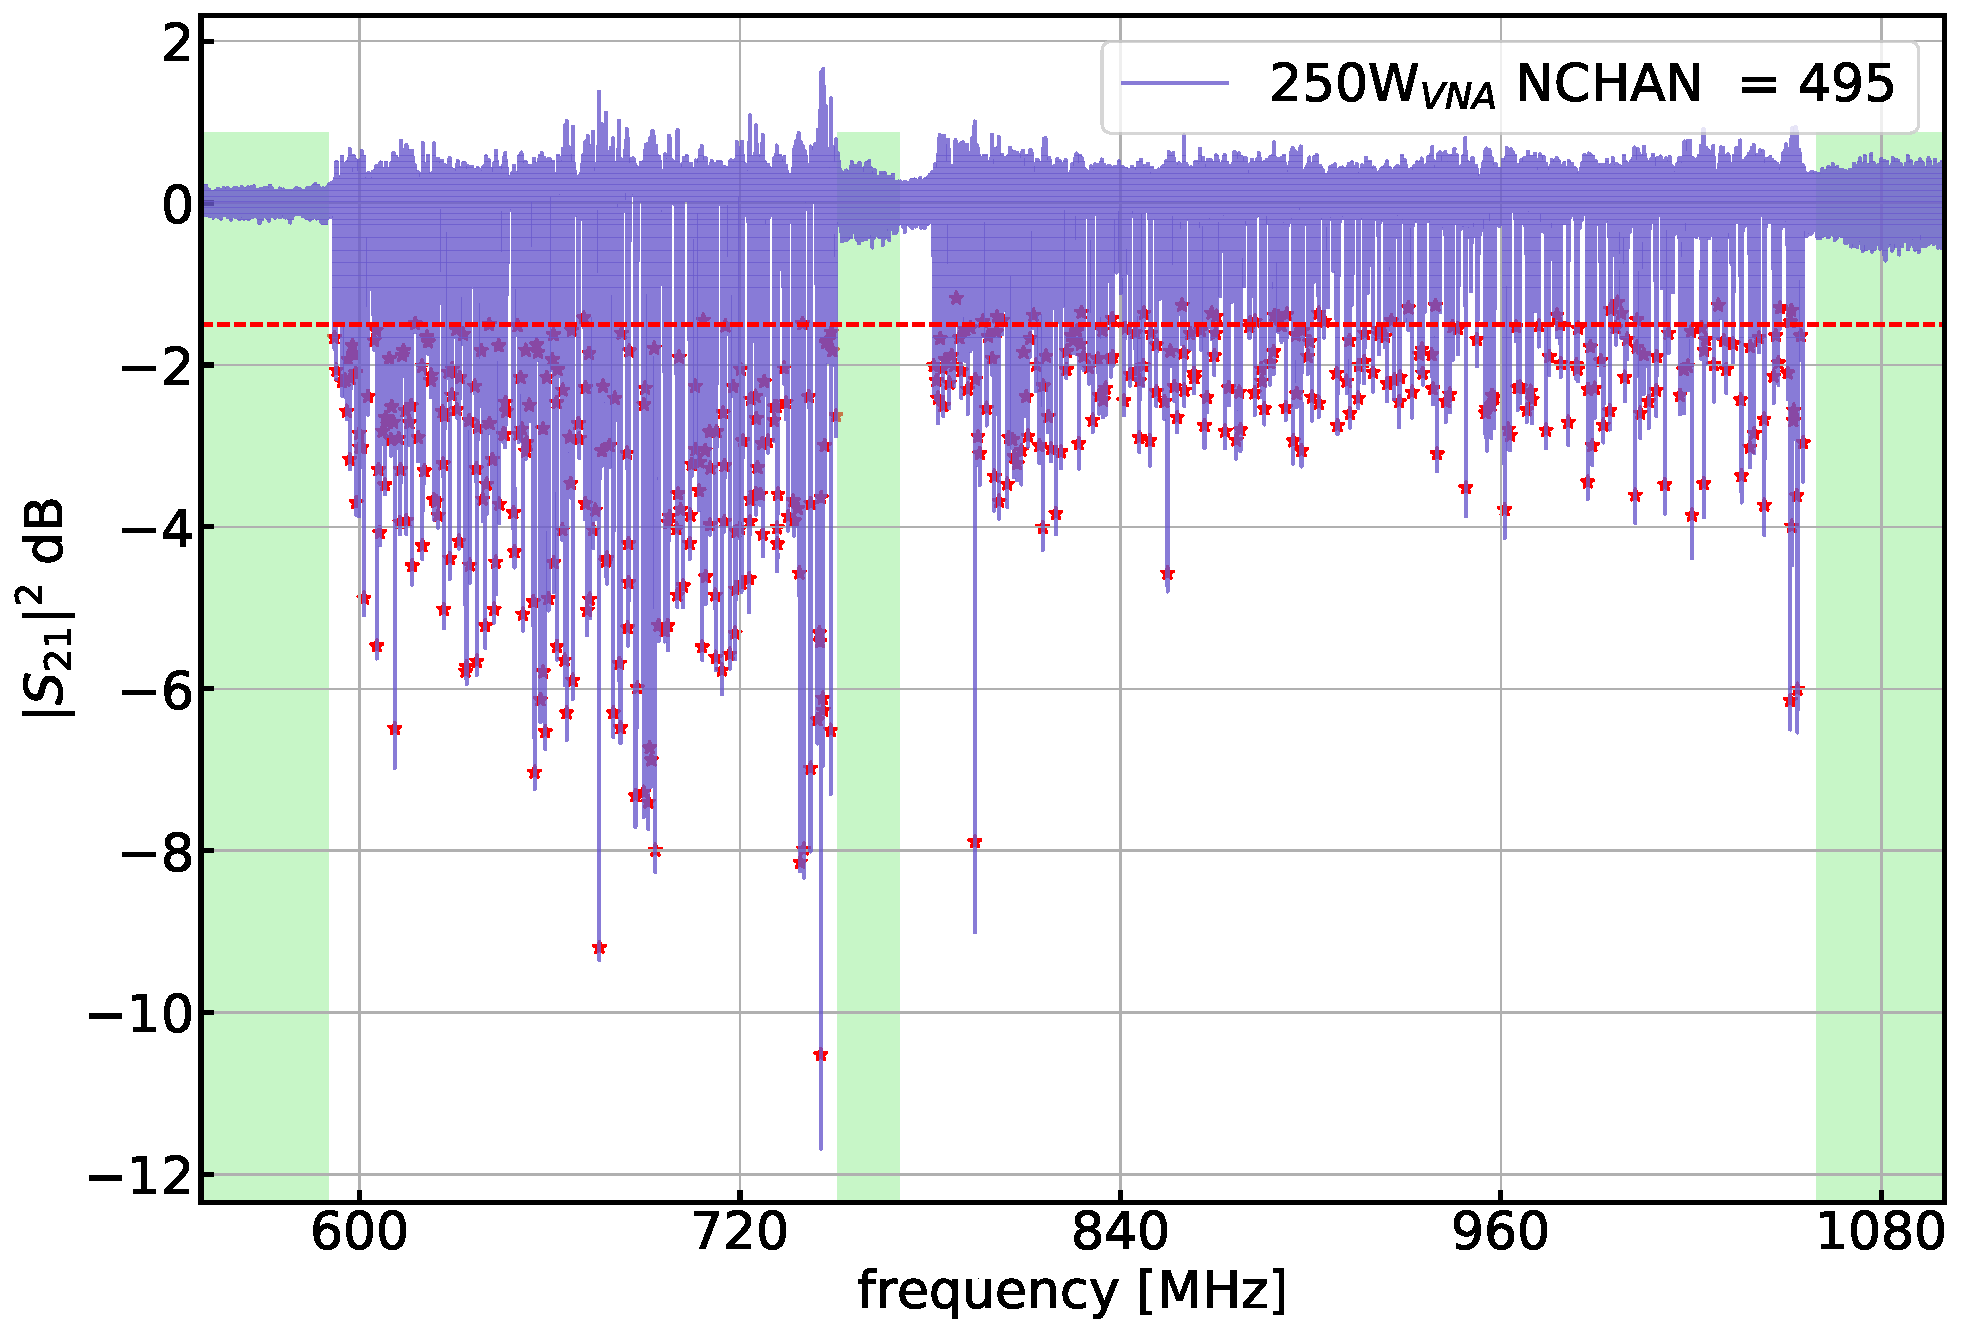
\includegraphics[width=0.68\textwidth]{figures/blast_data/sweeps/250W_May2018VNA_FK}
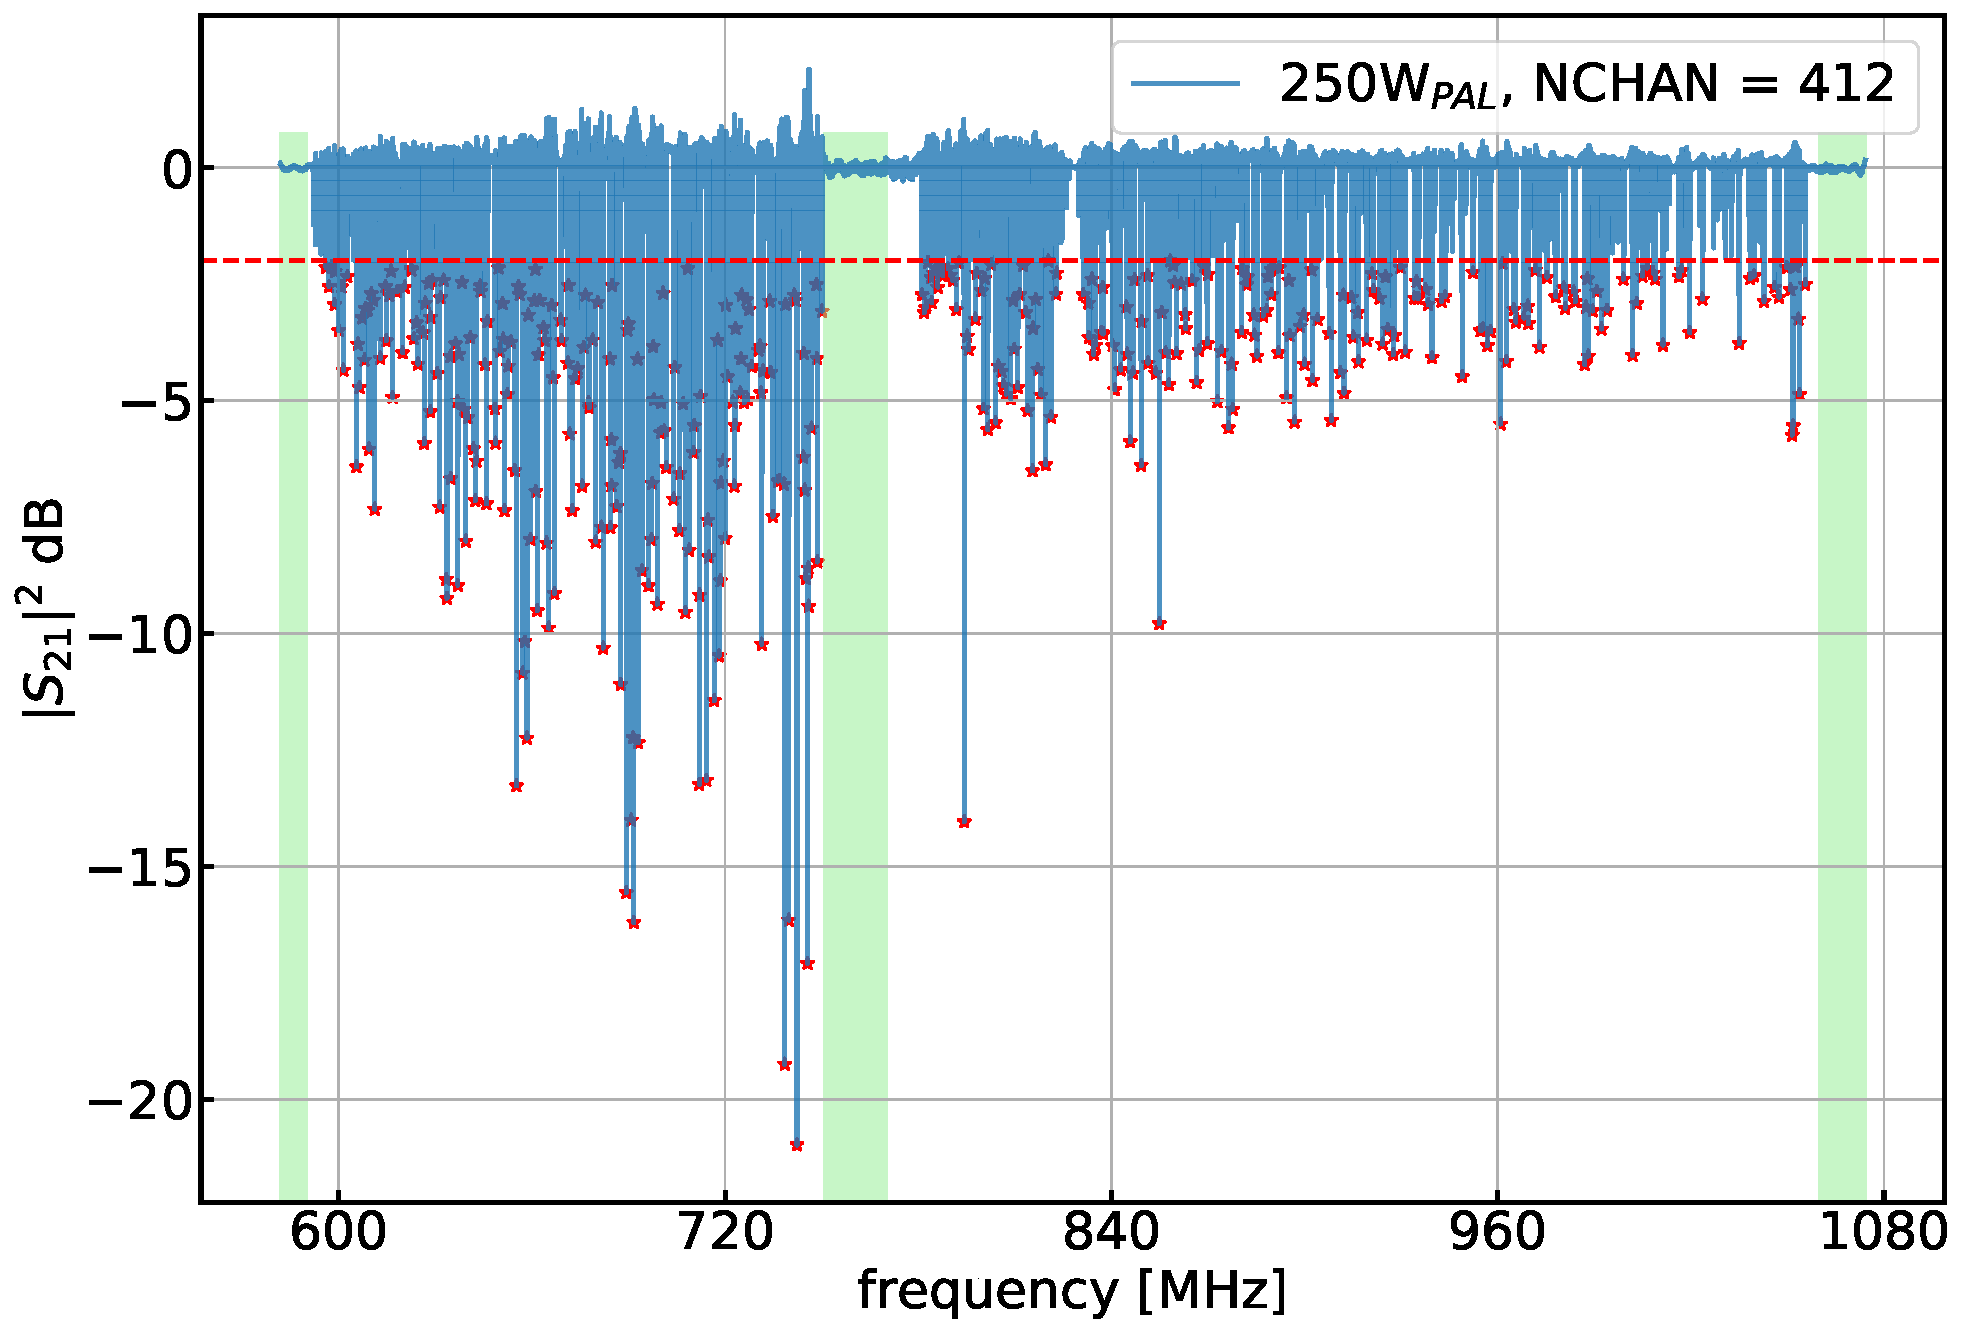
\includegraphics[width=0.68\textwidth]{figures/blast_data/sweeps/250W_PAL_FK}
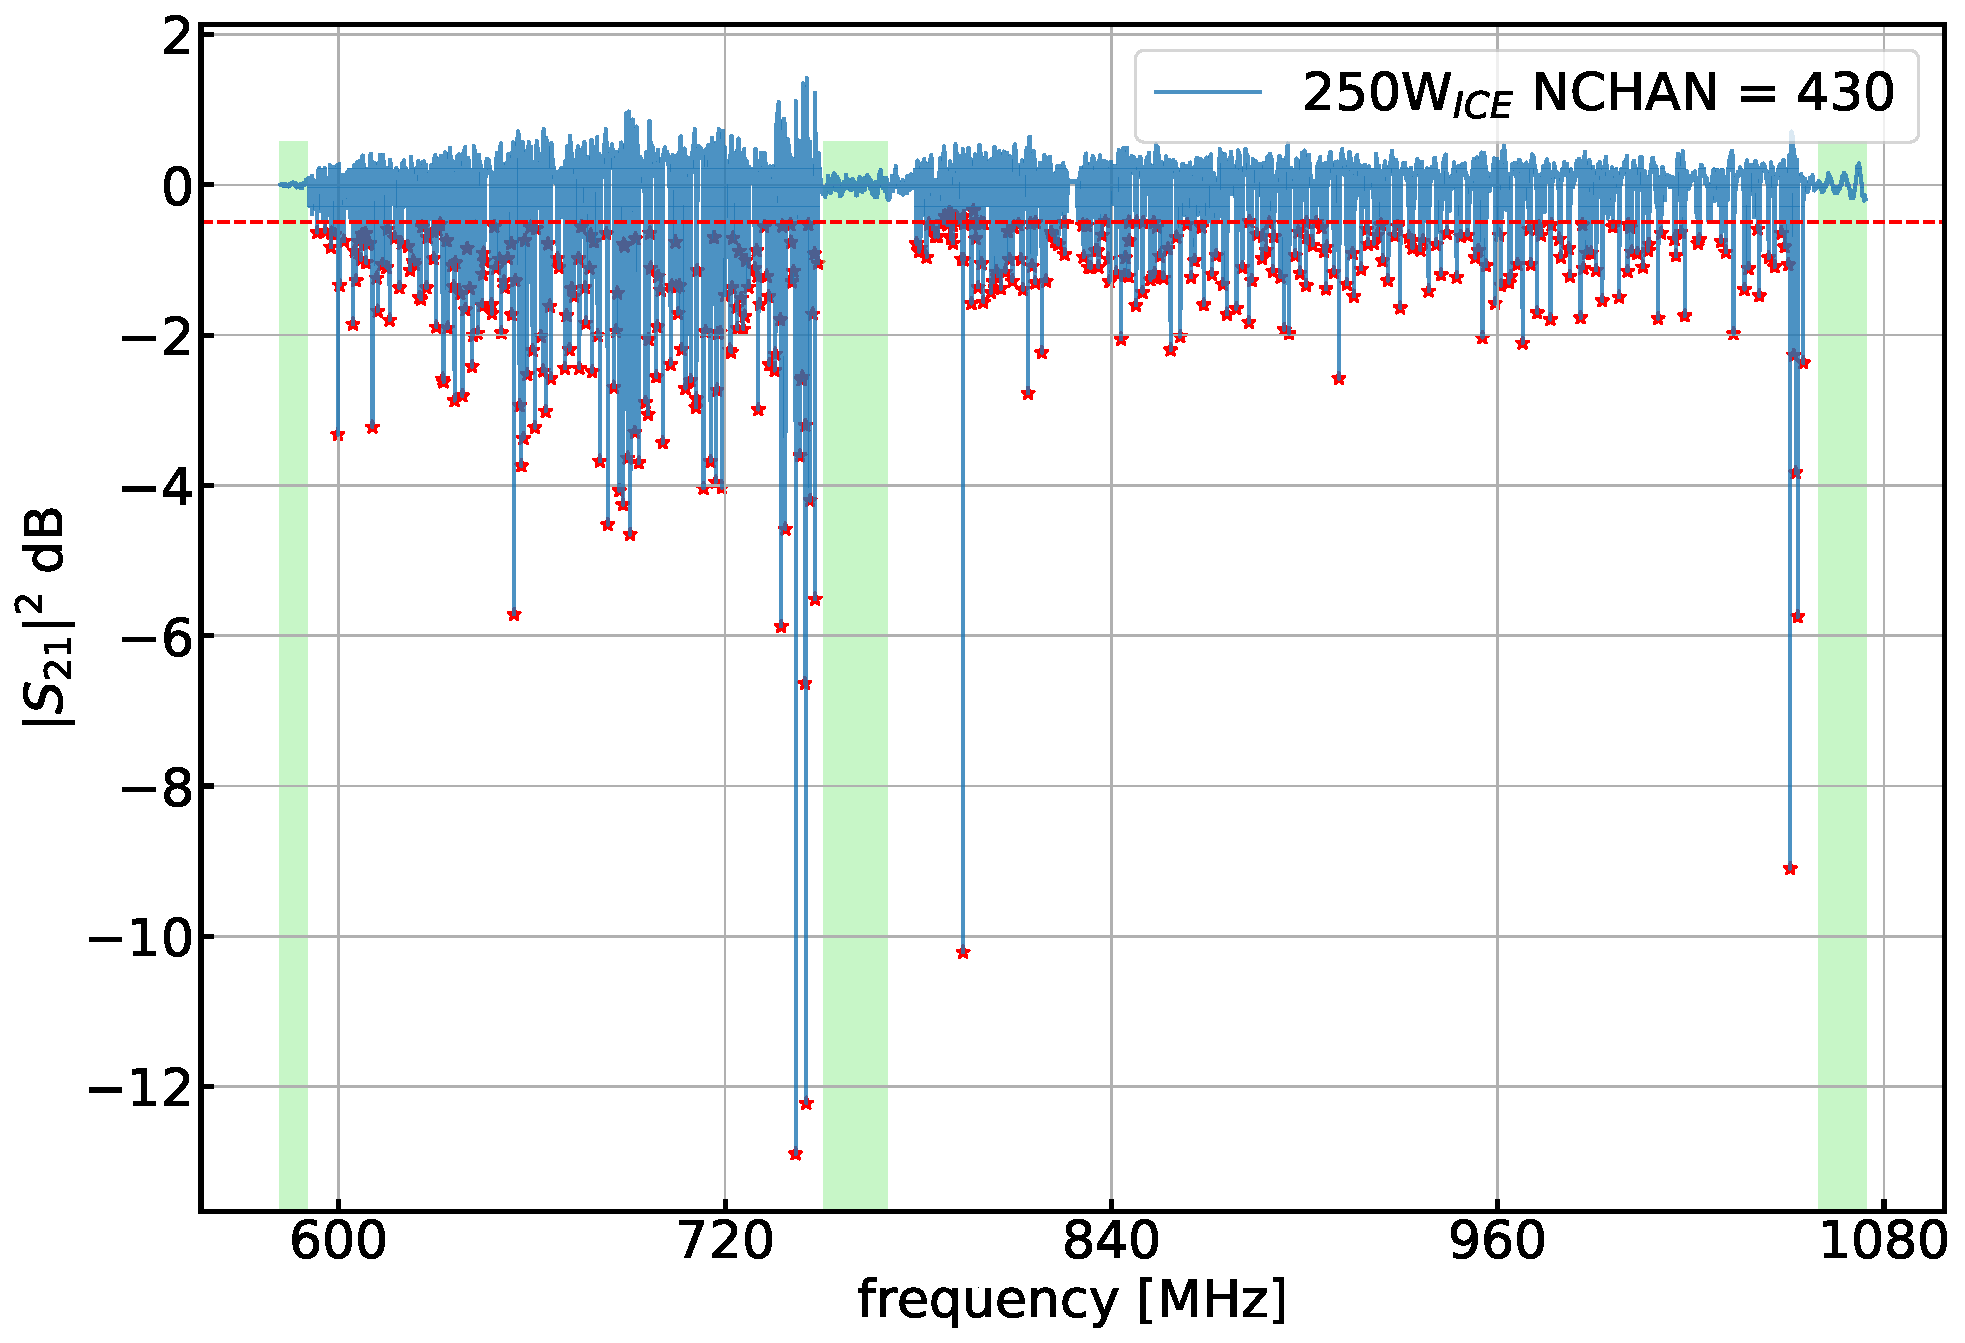
\includegraphics[width=0.68\textwidth]{figures/blast_data/sweeps/250W_ICE_FK}
\label{fig:250W FK}
\end{figure}

% 250 U

\begin{figure}[!p]
\centering
\caption[~250U array KID-finding results.]{250U array KID-finding results for a VNA sweep (top) and ROACH2 sweeps from Palestine (middle) and the ice (bottom).}
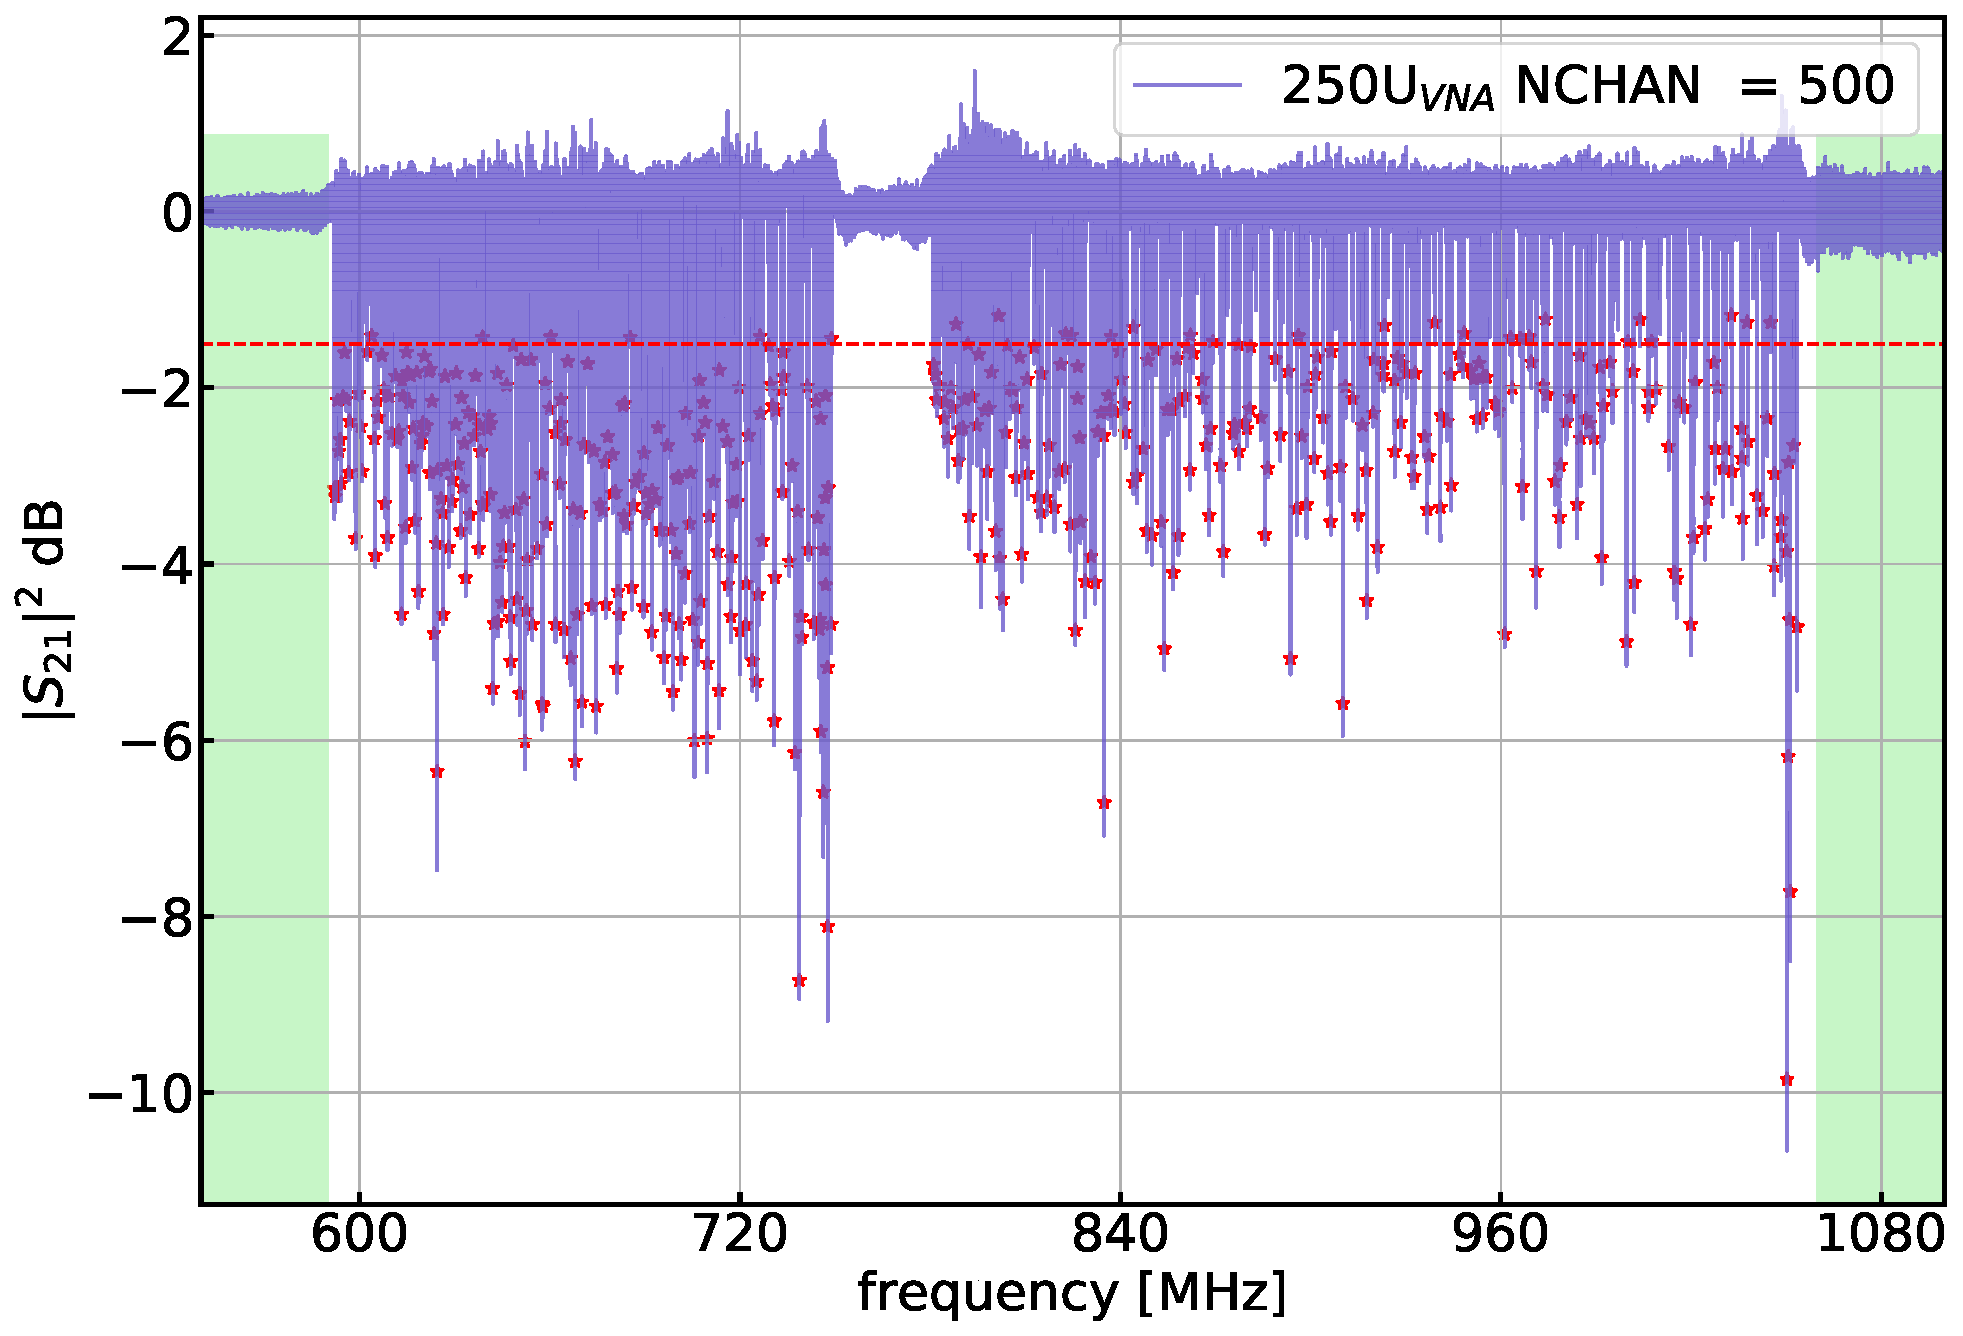
\includegraphics[width=0.68\textwidth]{figures/blast_data/sweeps/250U_May2018VNA_FK}
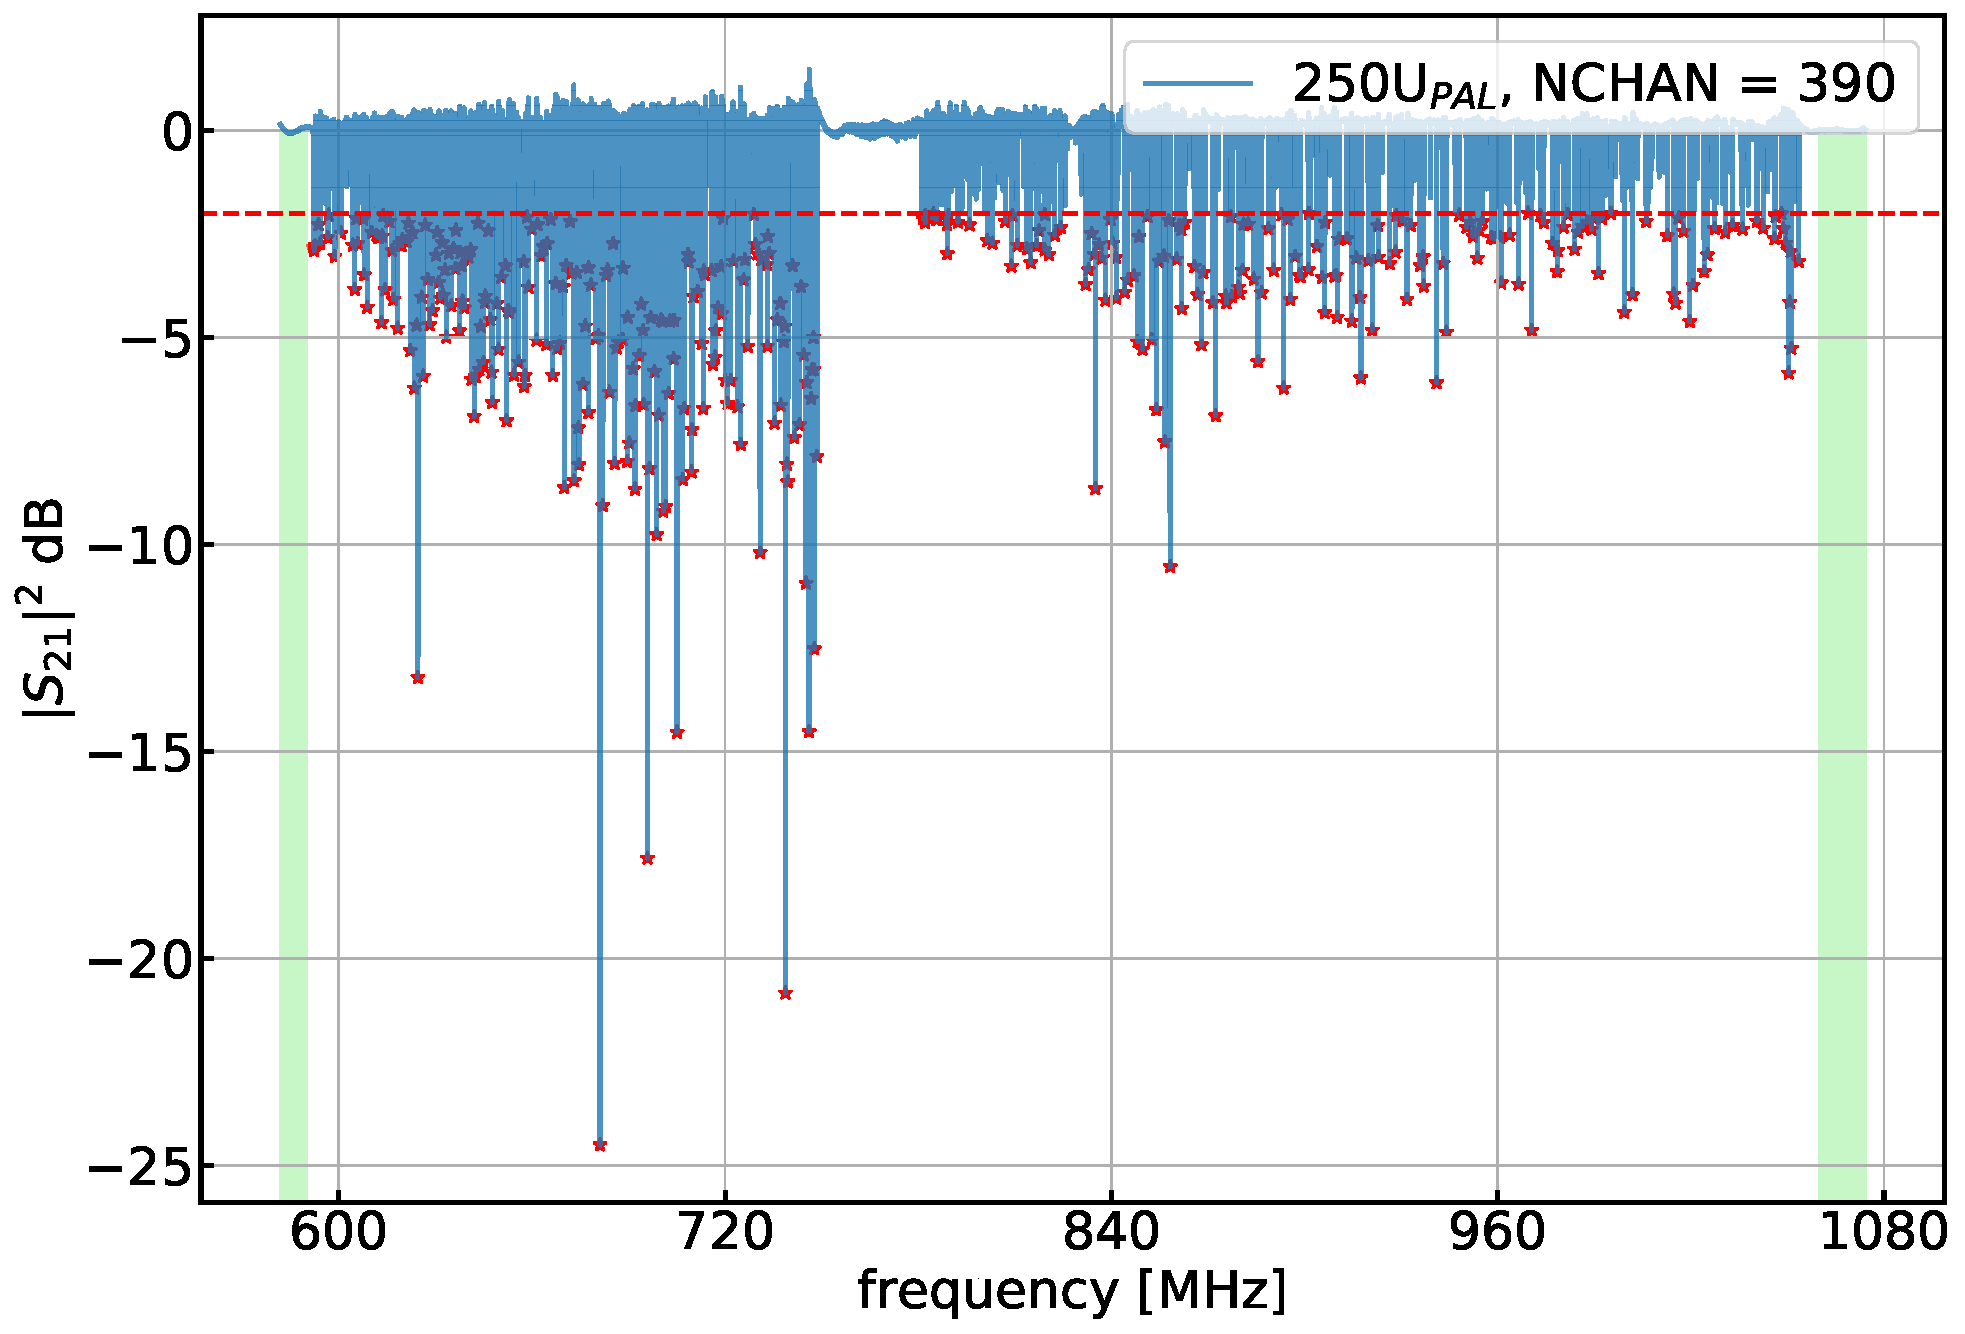
\includegraphics[width=0.68\textwidth]{figures/blast_data/sweeps/250U_PAL_FK}
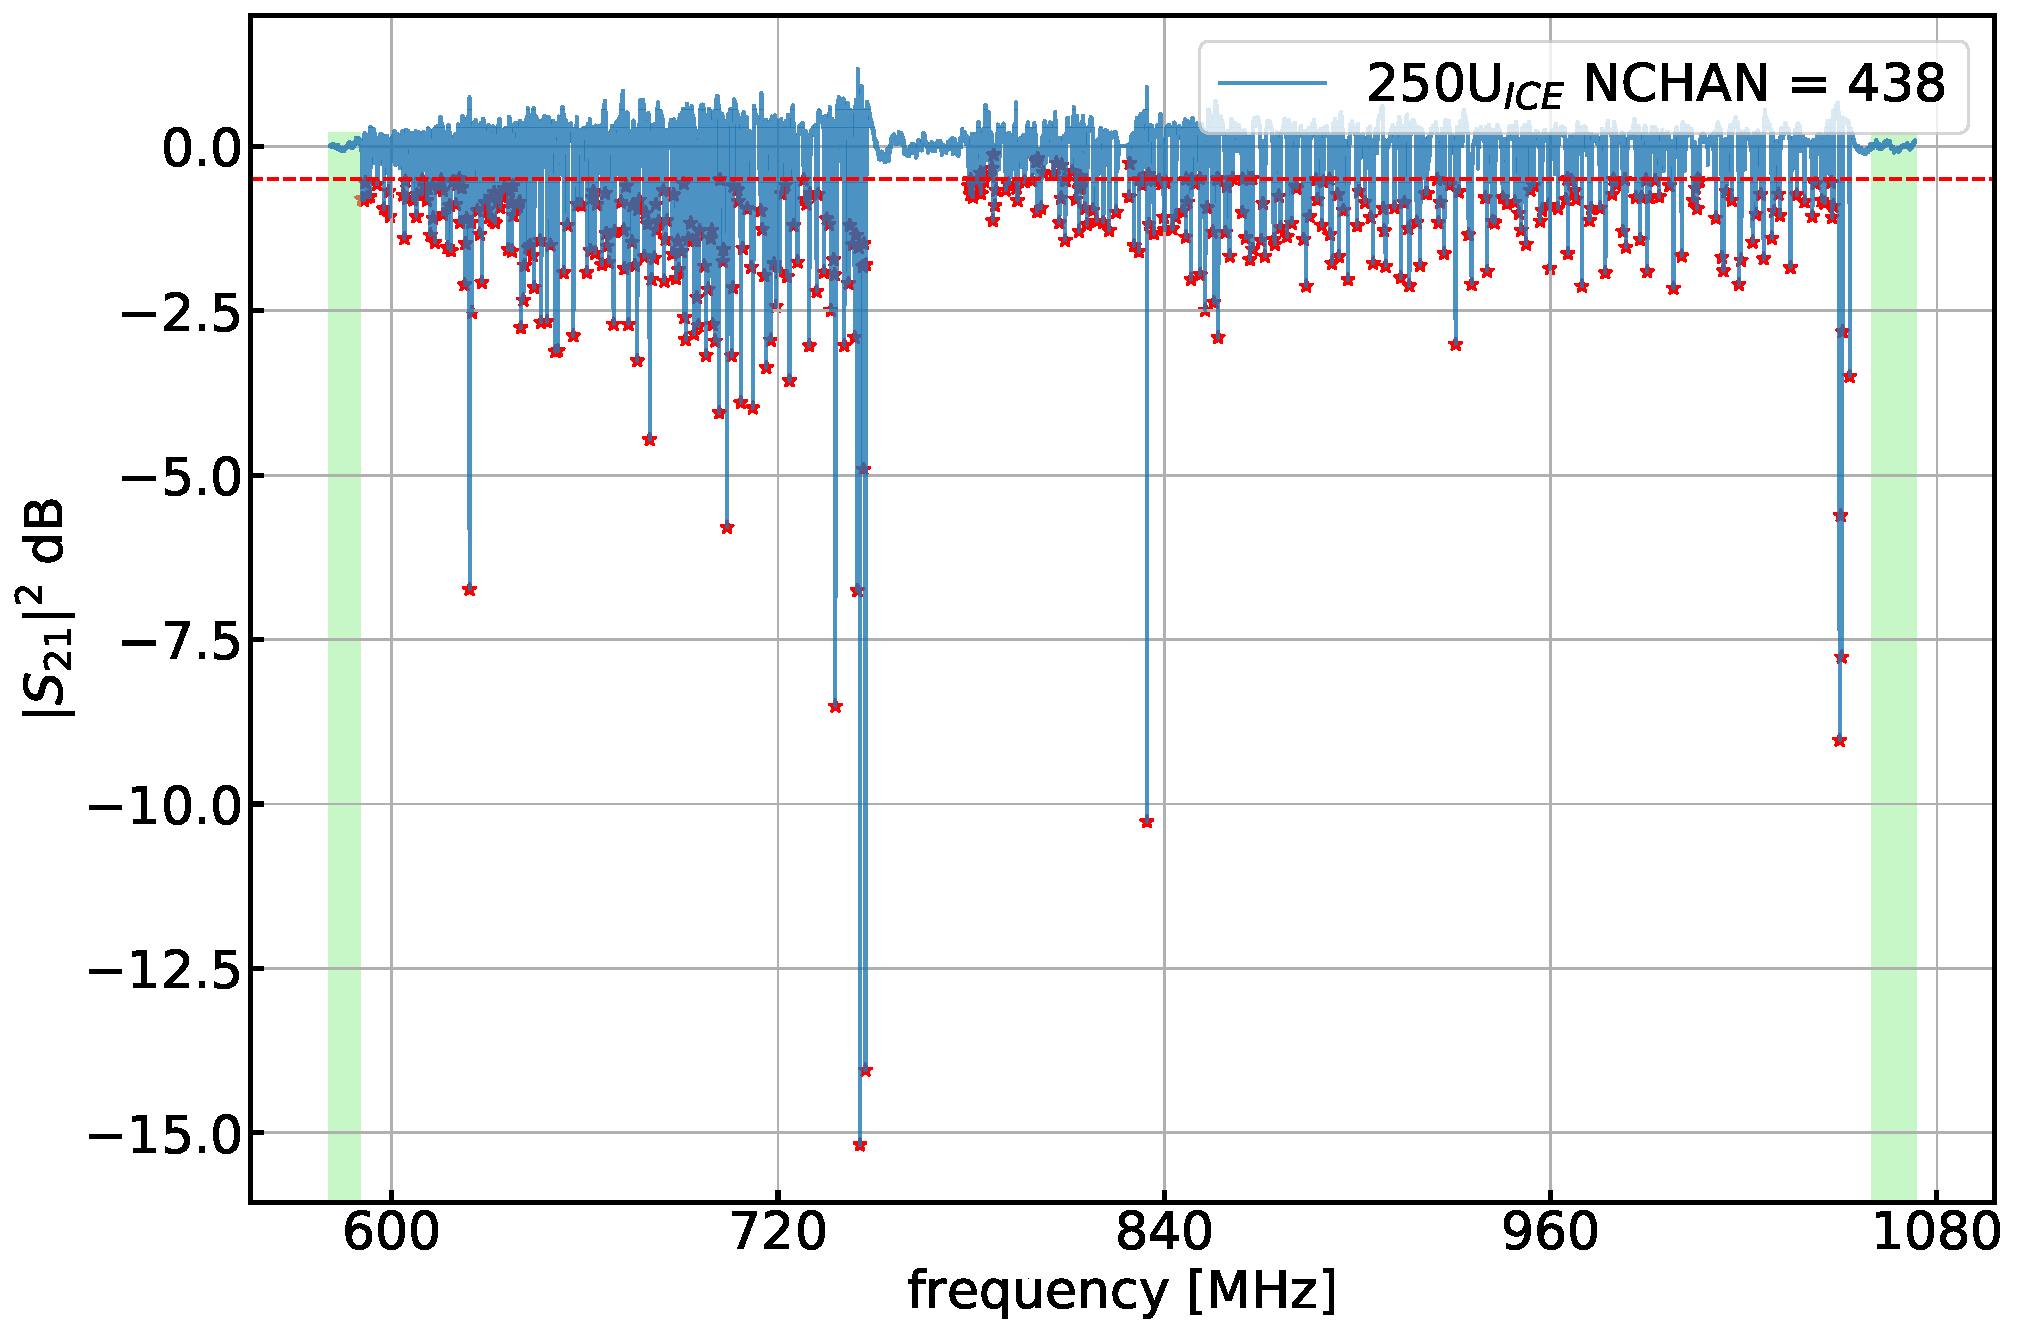
\includegraphics[width=0.68\textwidth]{figures/blast_data/sweeps/250U_ICE_FK}
\label{fig:250U FK}
\end{figure}

% 250 V

\begin{figure}[!p]
\centering
\caption[~250V array KID-finding results.]{250V array KID-finding results for a VNA sweep (top) and a ROACH2 sweep from Palestine (bottom).}
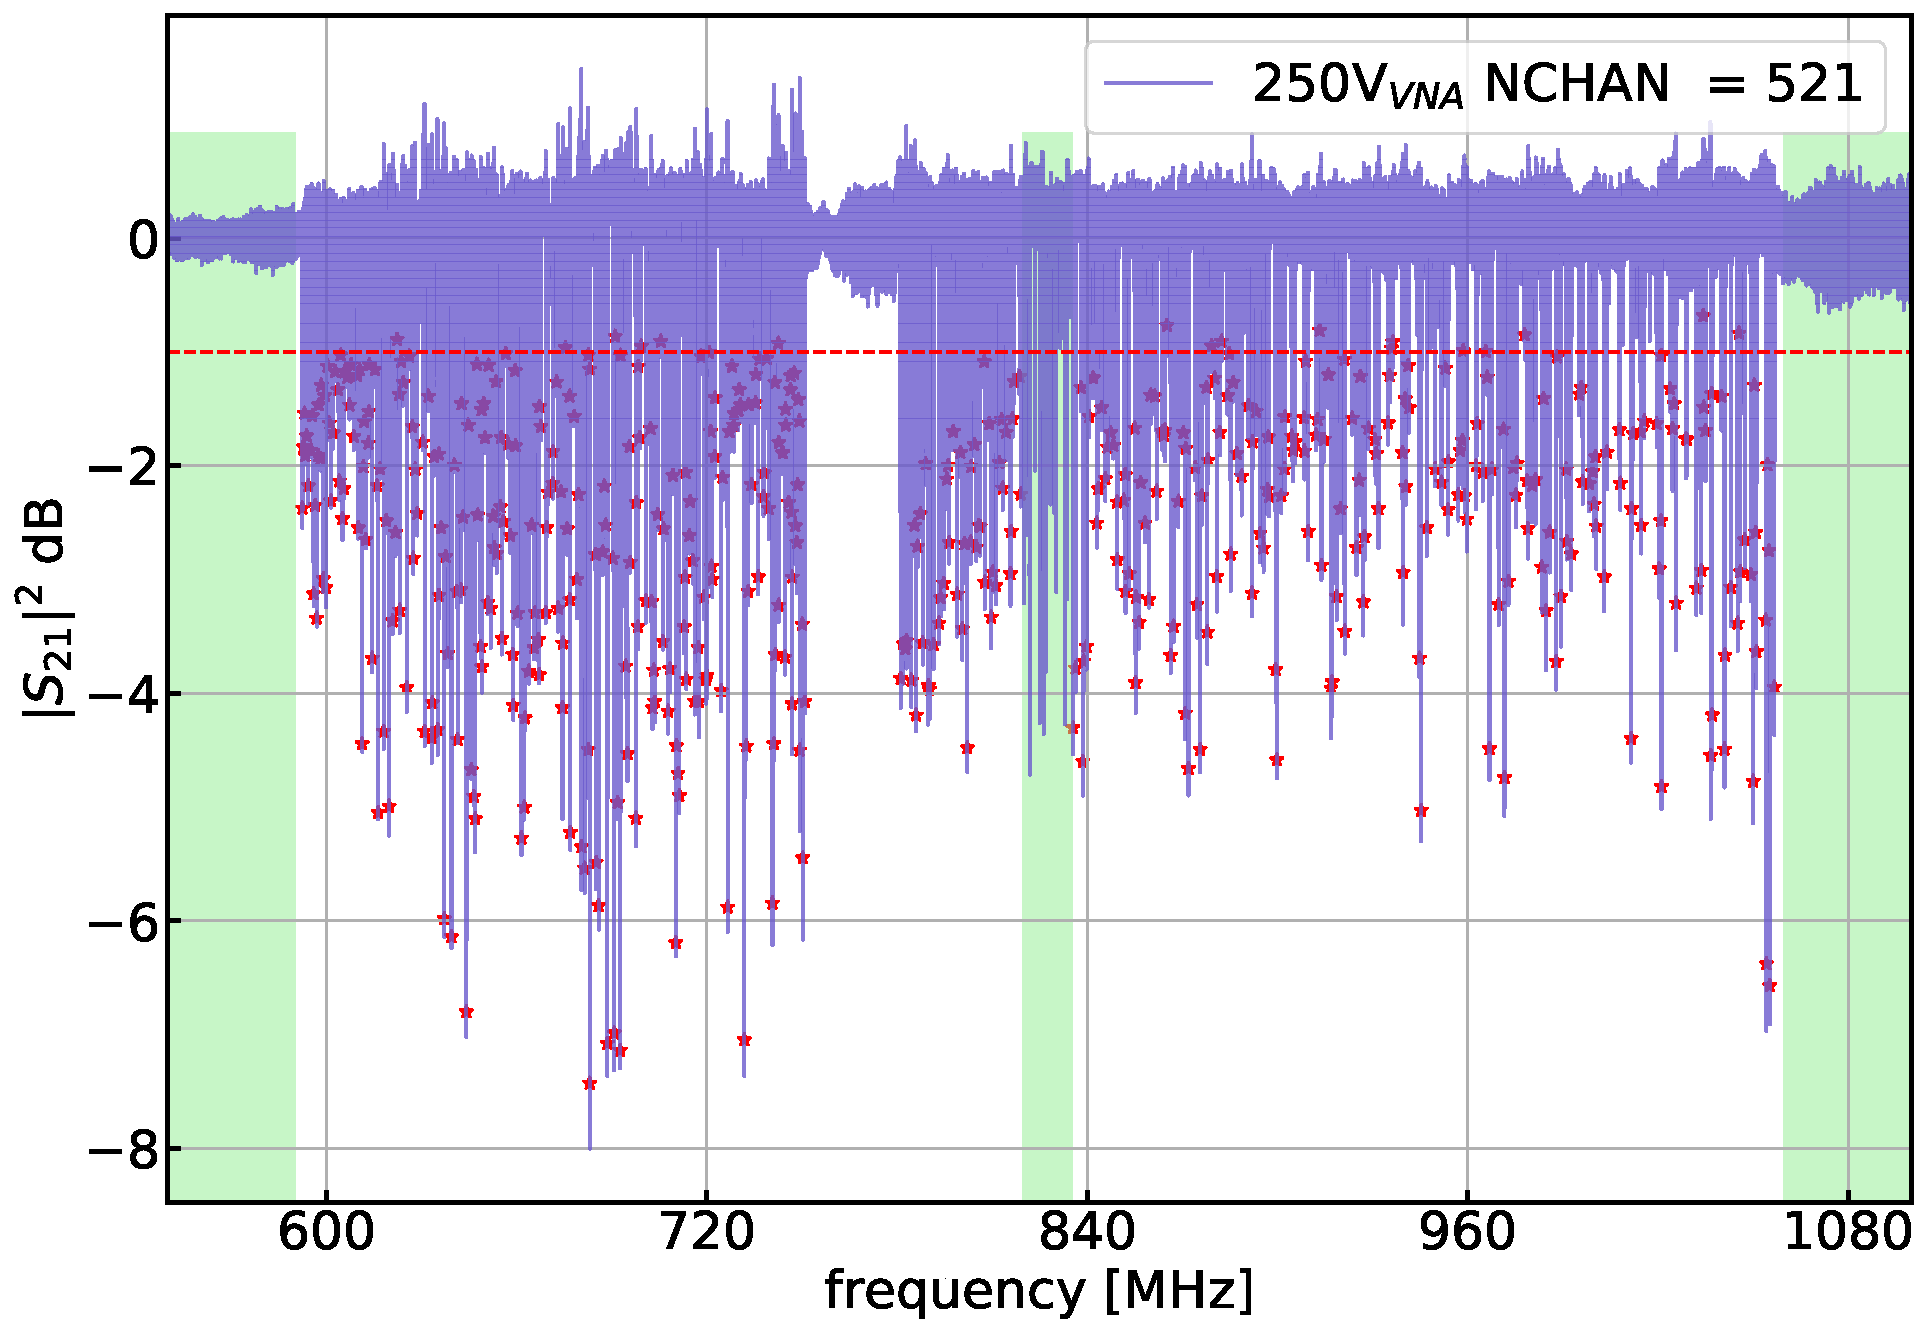
\includegraphics[width=0.68\textwidth]{figures/blast_data/sweeps/250V_May2018VNA_FK}
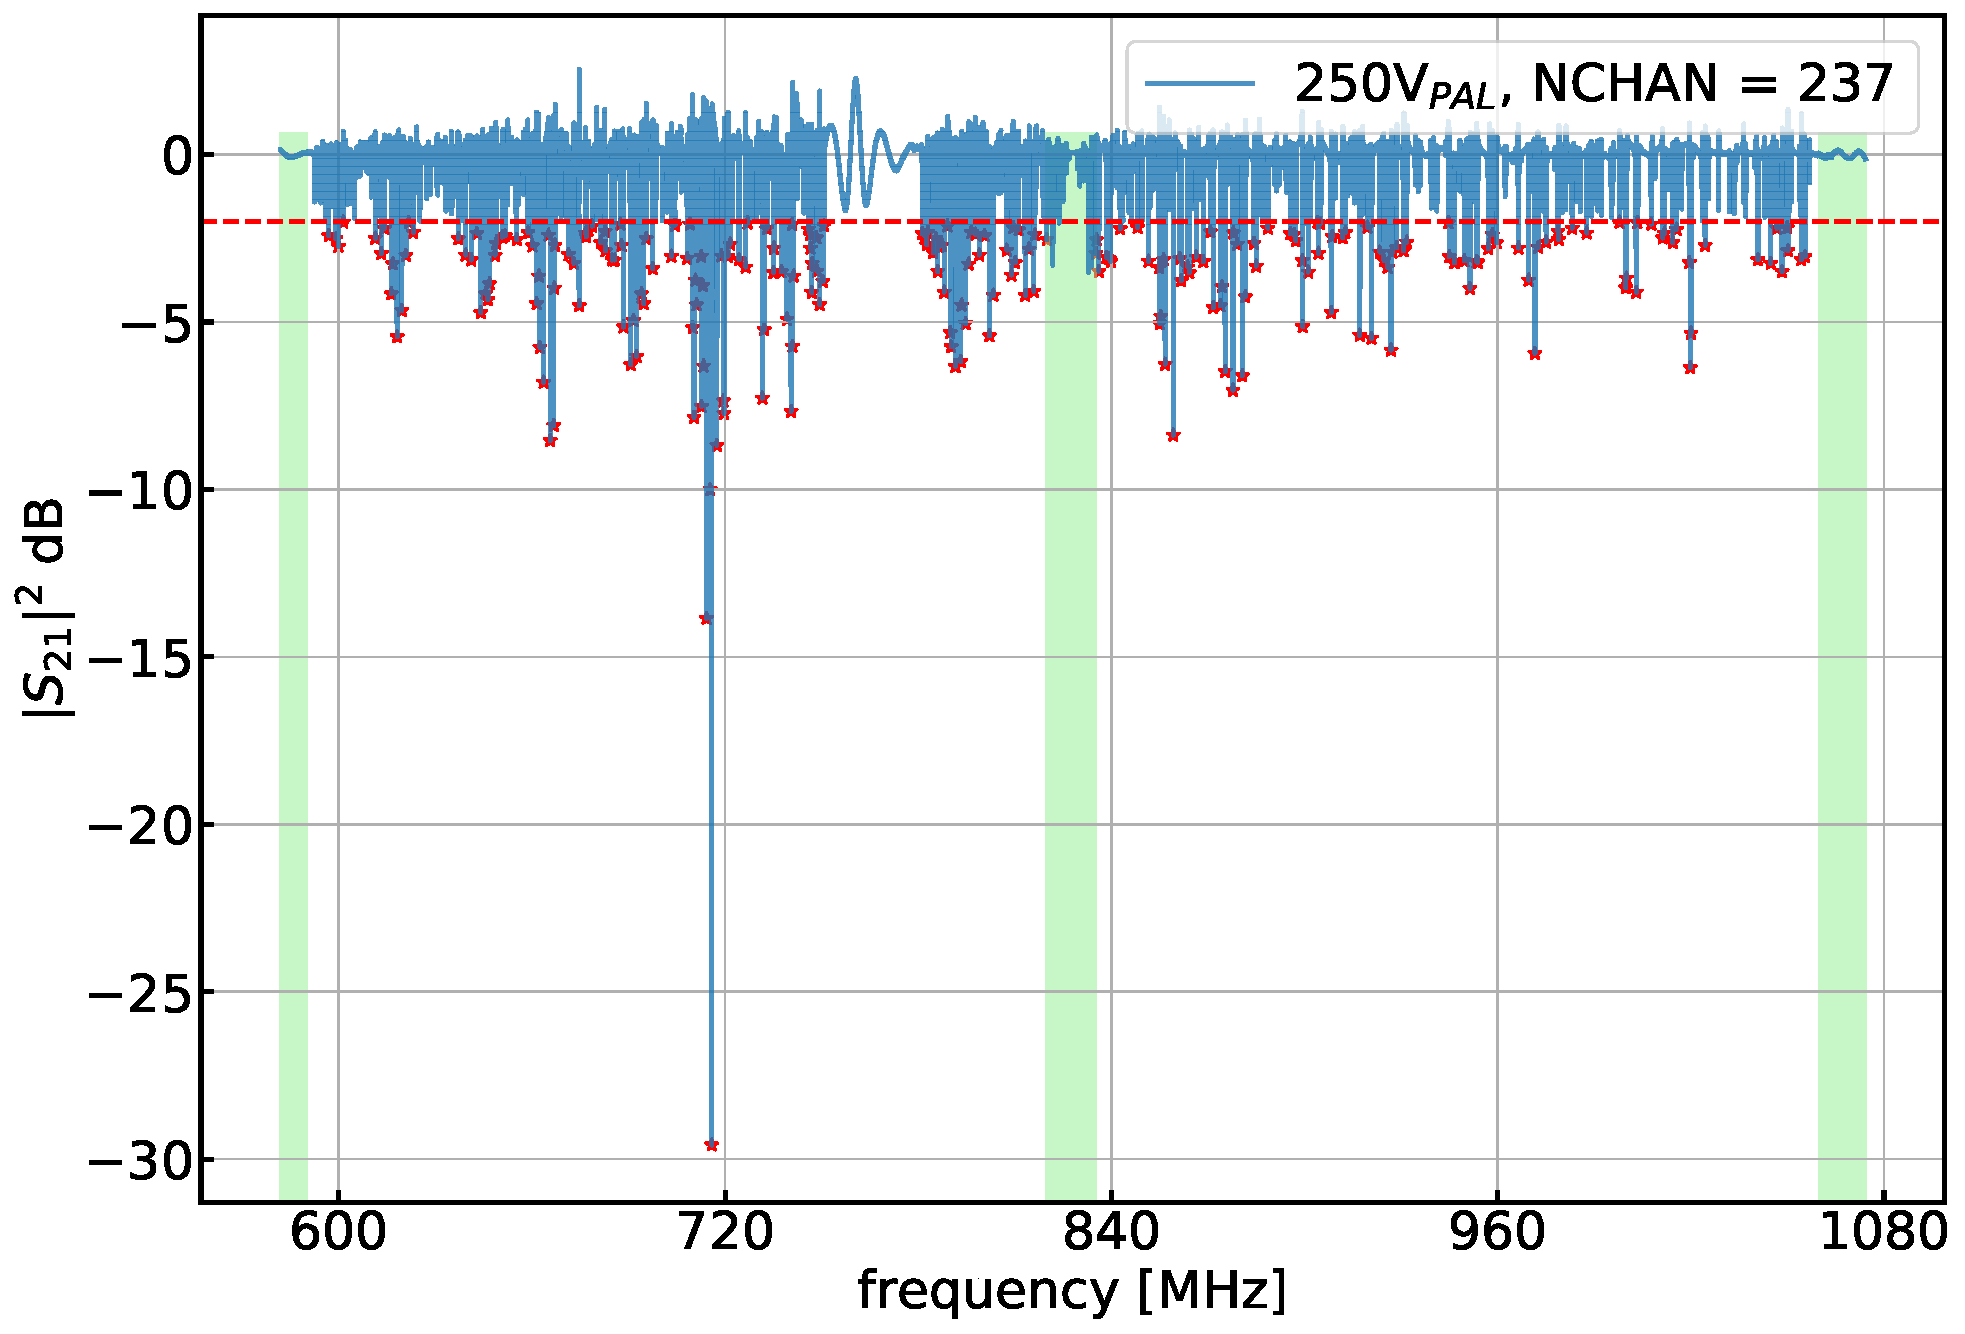
\includegraphics[width=0.68\textwidth]{figures/blast_data/sweeps/250V_PAL_FK}
\label{fig:250V FK}
\end{figure}

% 500
\begin{figure}[!p]
\centering
\caption[~\macrocapwrap{500~$\upmu$m} array KID-finding results.]{500~$\upmu$m array KID-finding results for a VNA sweep (top) and ROACH2 sweeps from Palestine (middle) and the ice (bottom).}
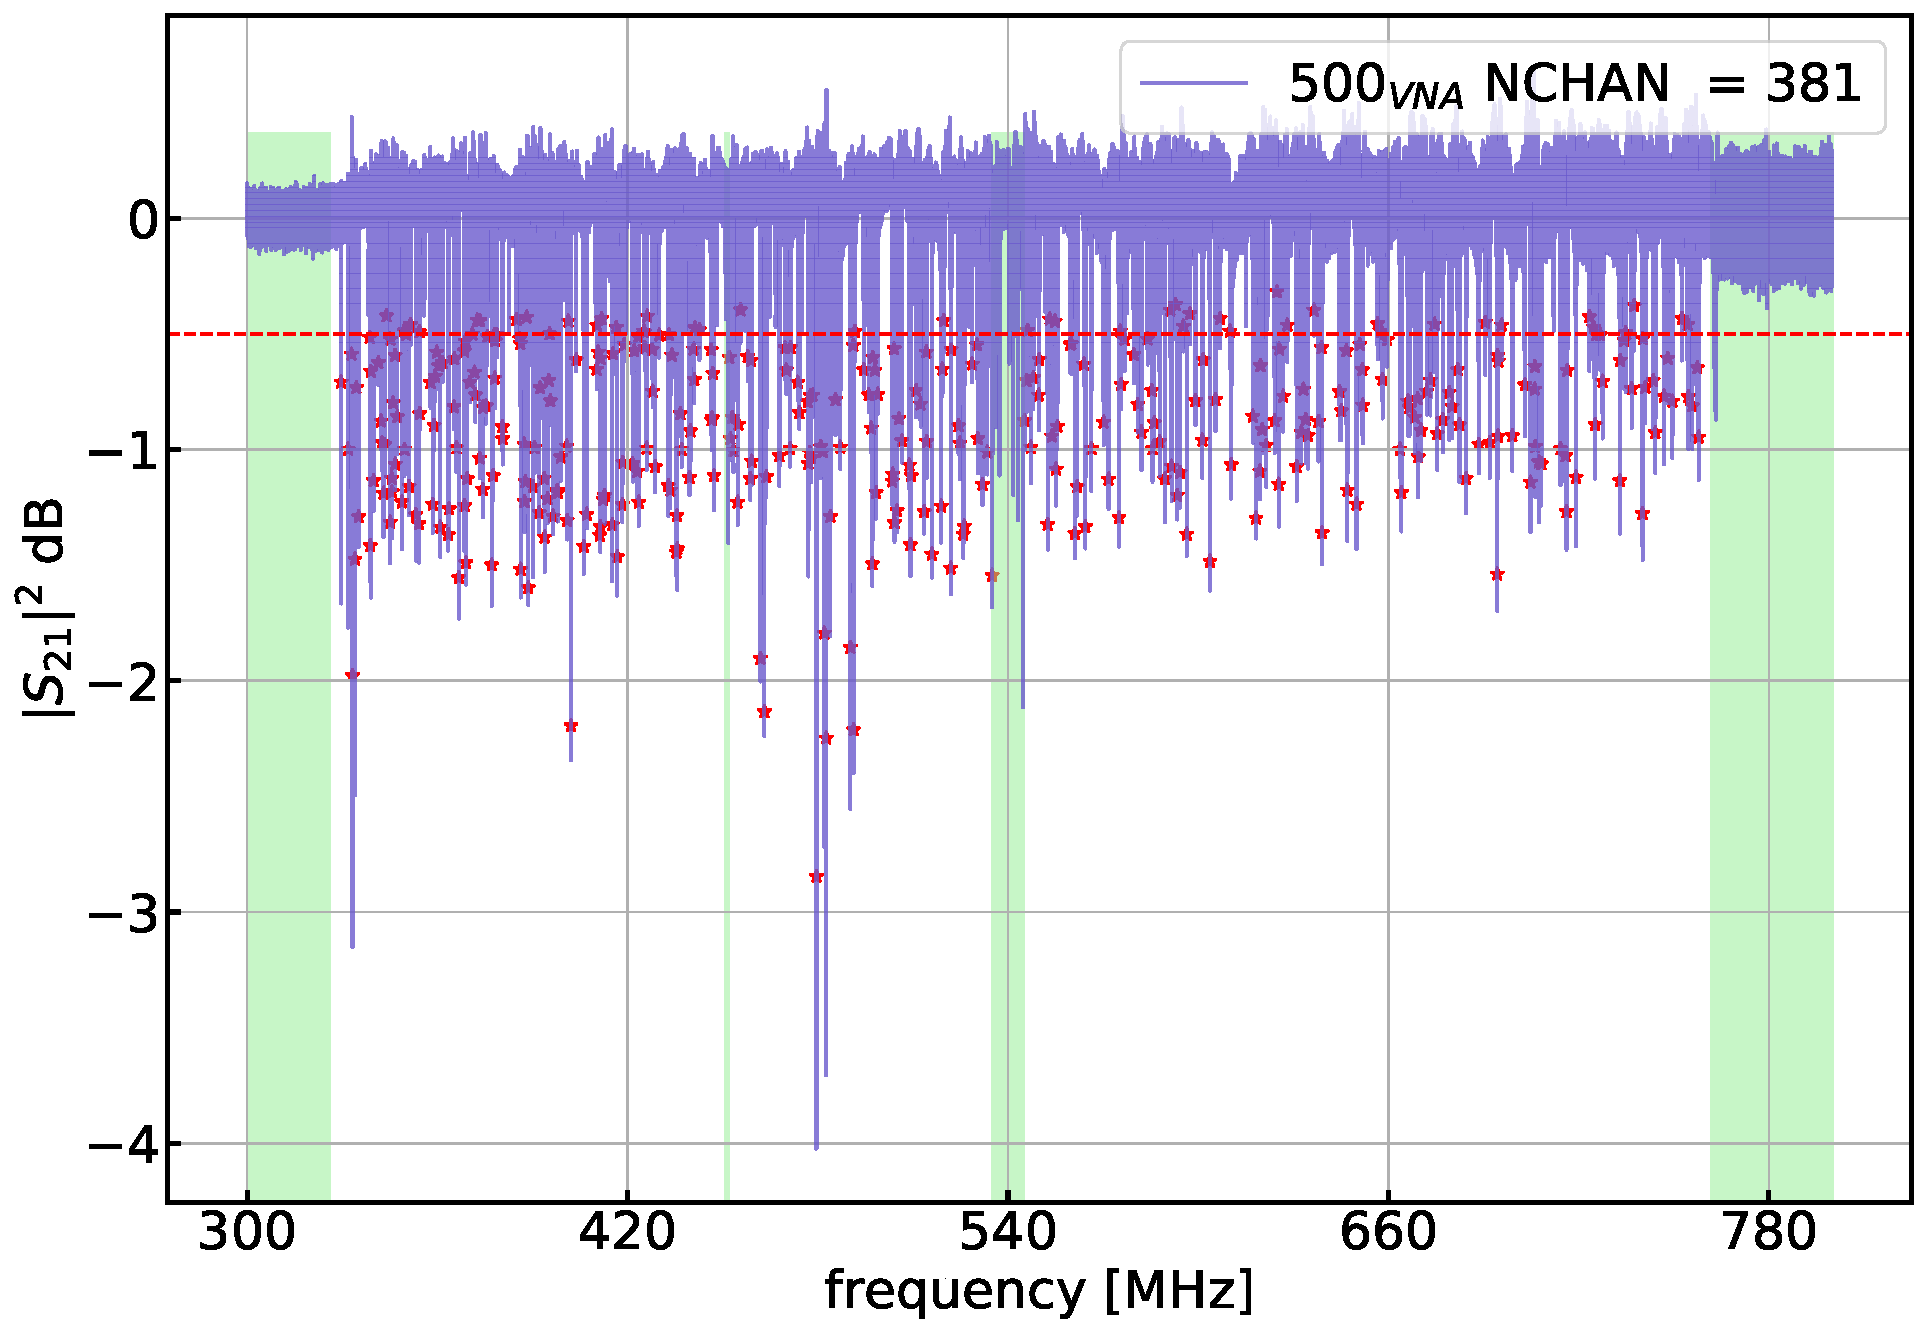
\includegraphics[width=0.68\textwidth]{figures/blast_data/sweeps/500_May2018VNA_FK}
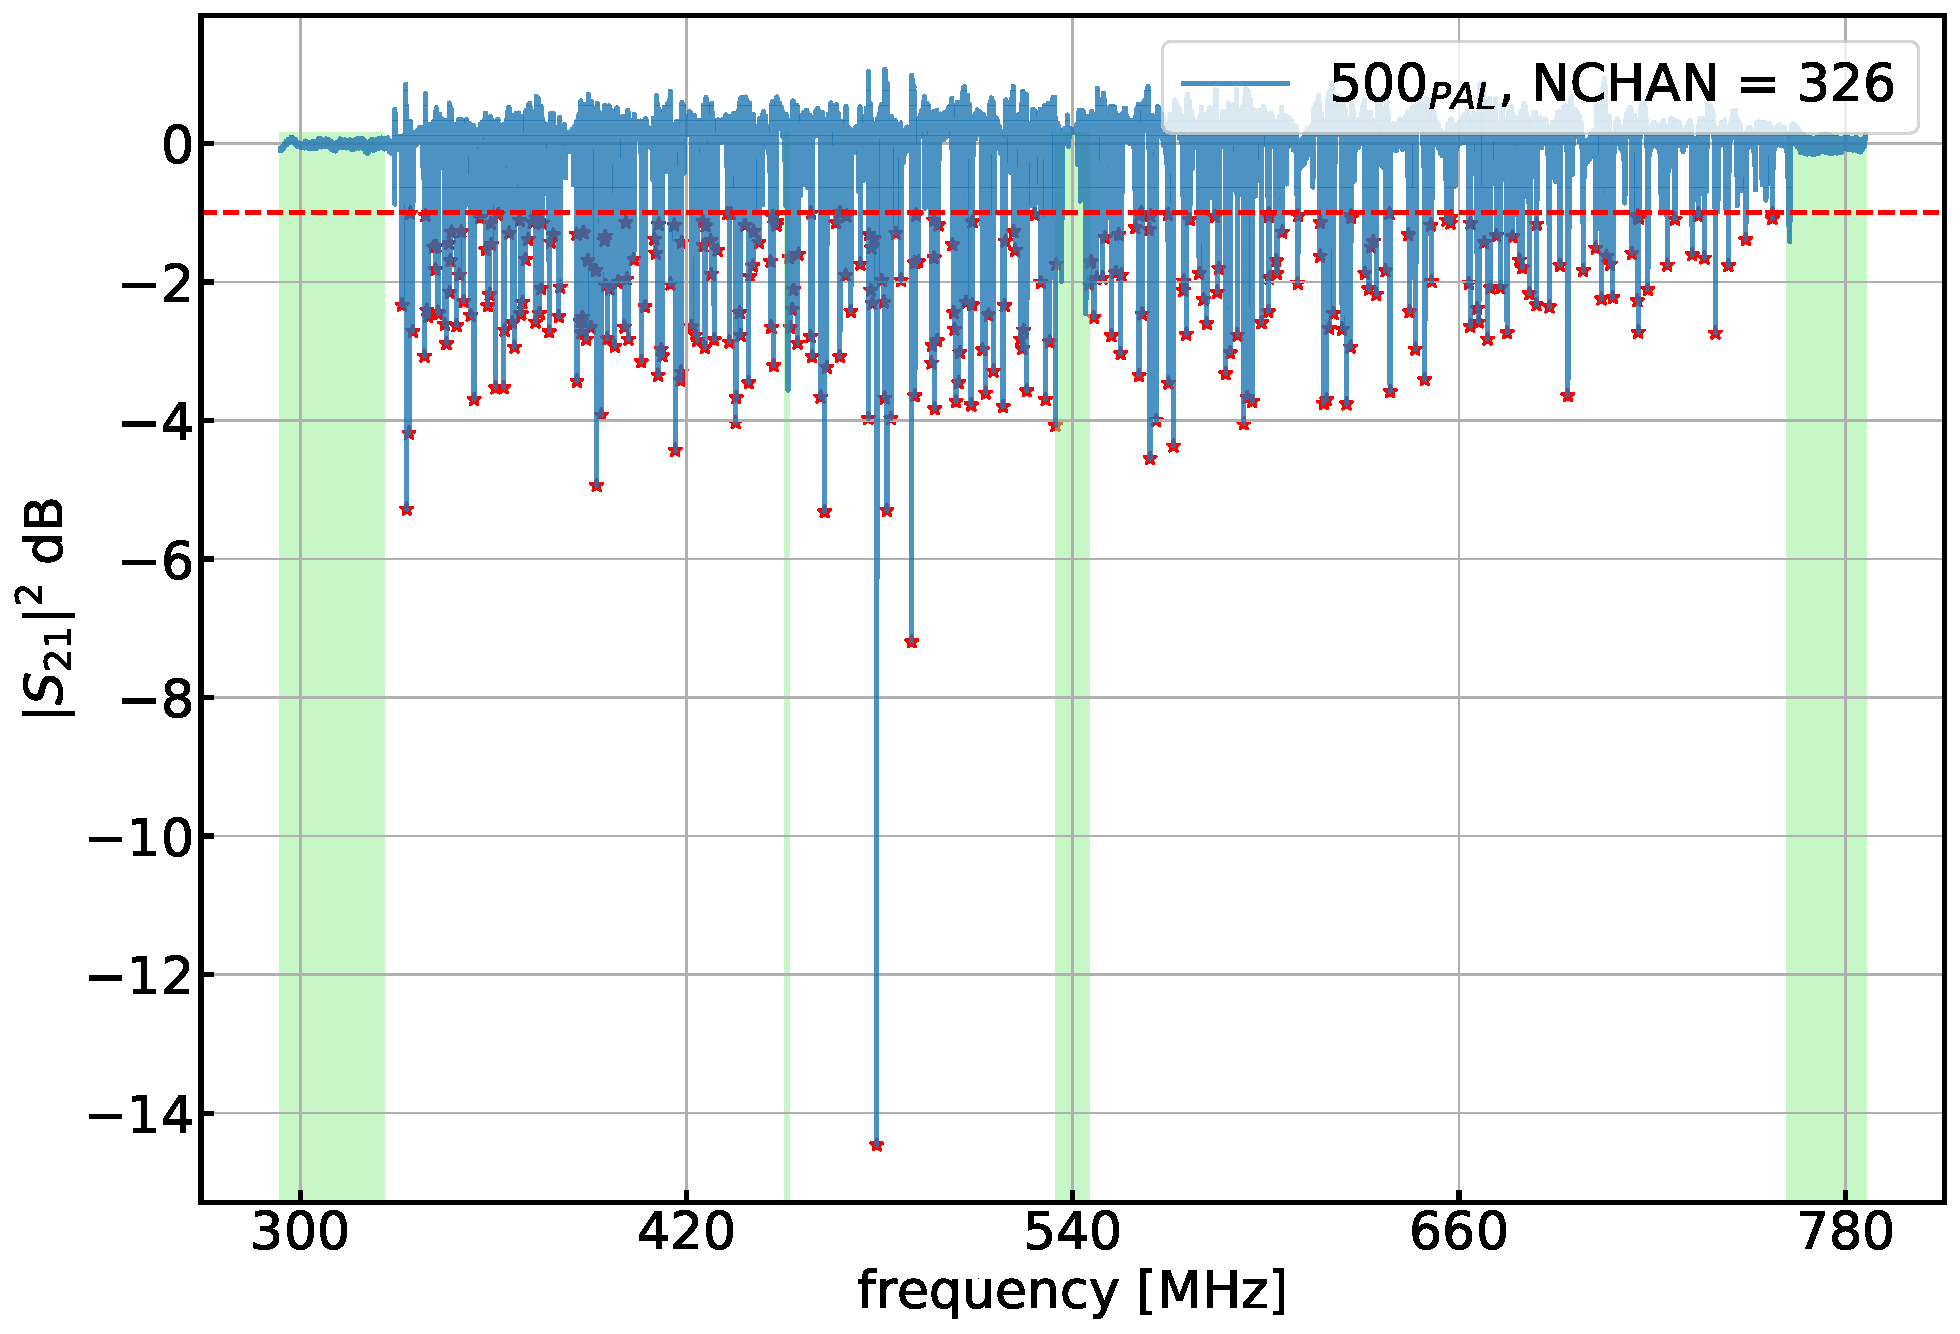
\includegraphics[width=0.68\textwidth]{figures/blast_data/sweeps/500_PAL_FK}
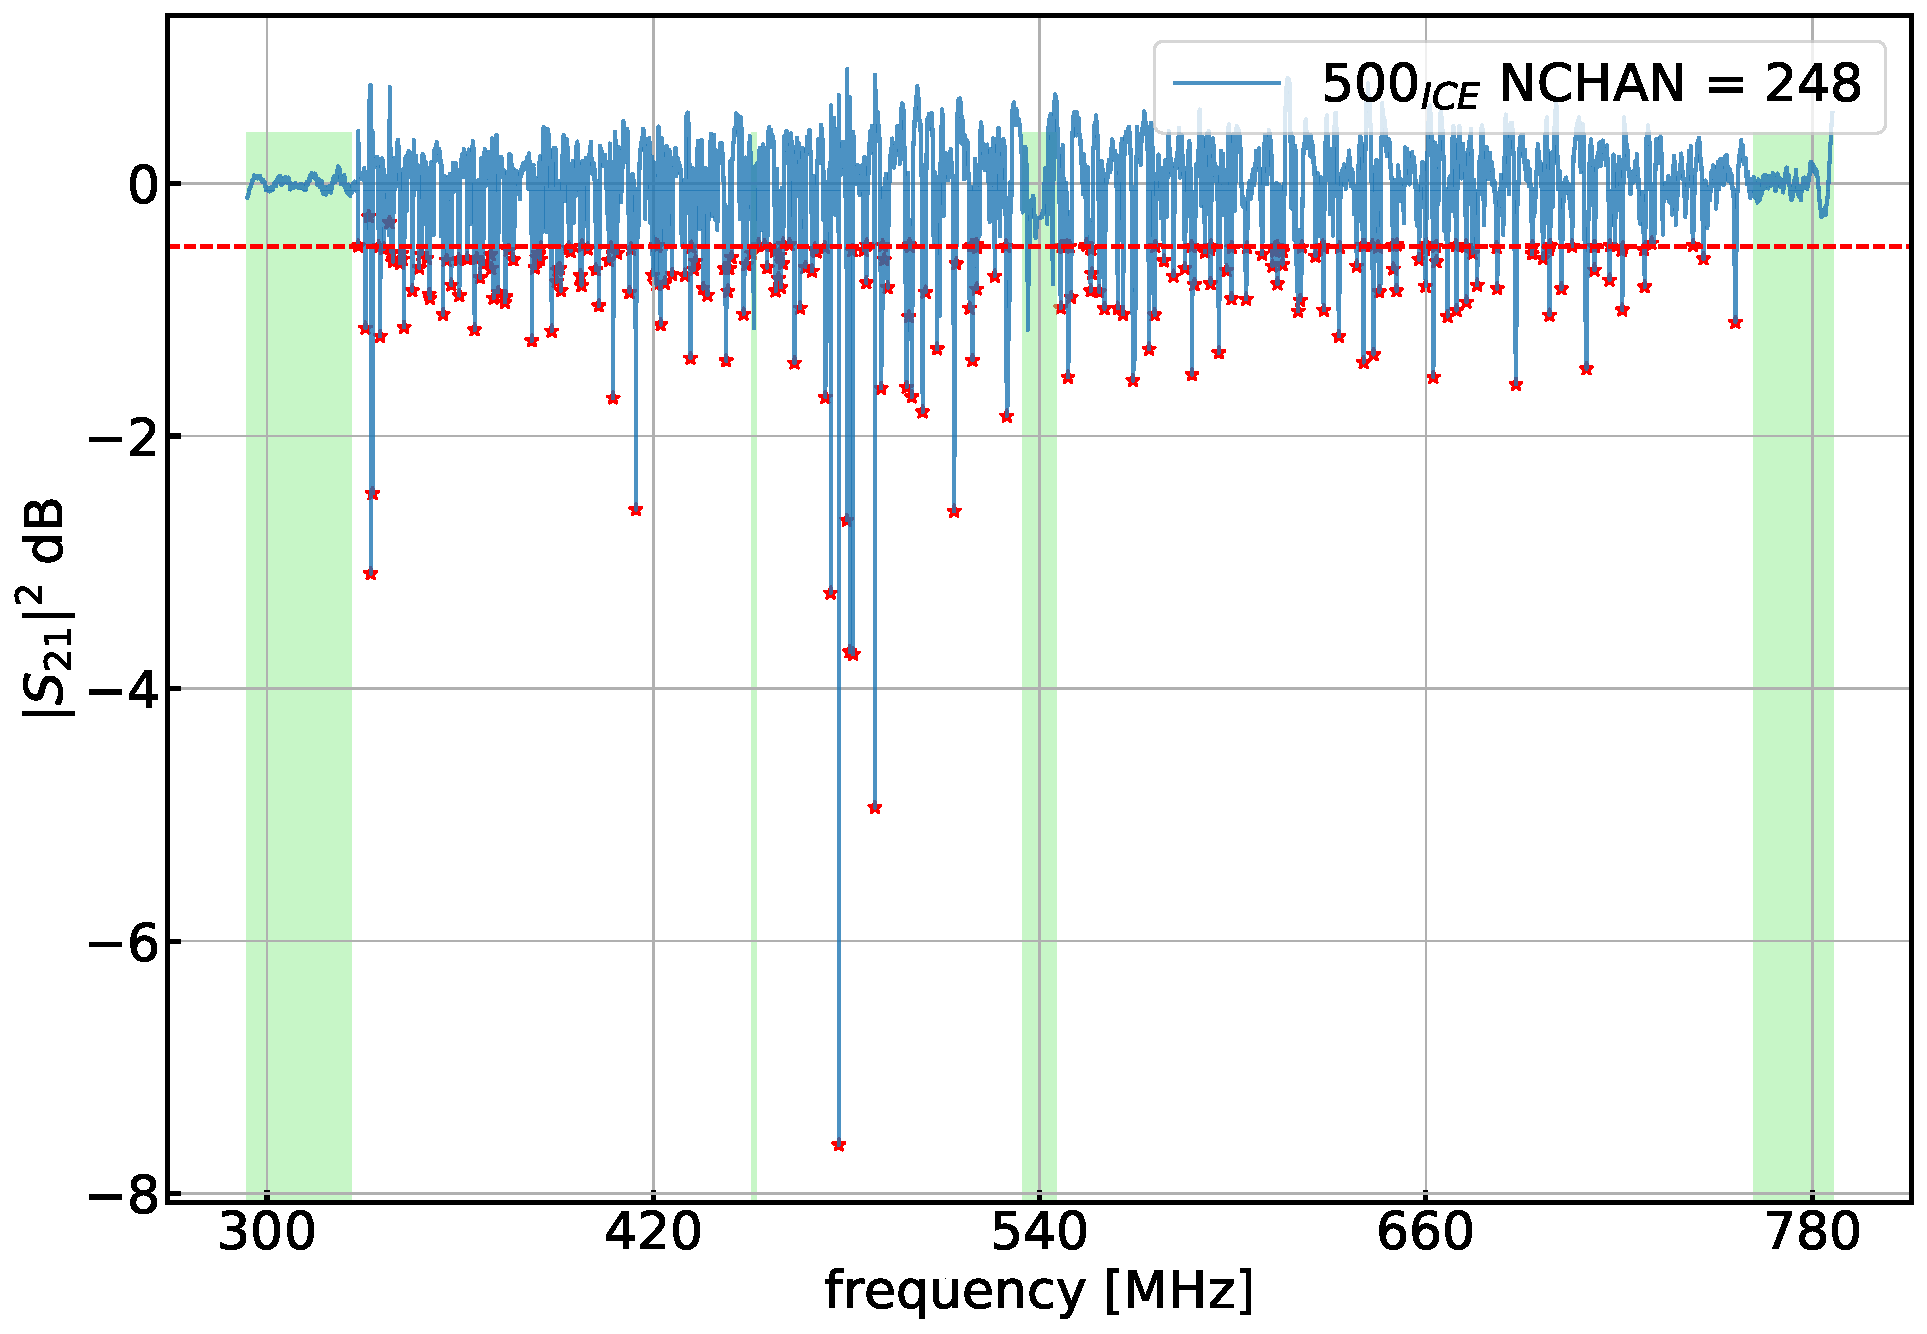
\includegraphics[width=0.68\textwidth]{figures/blast_data/sweeps/500_ICE_FK}
\label{fig:500 VNA FK}
\end{figure}

\subsection{Target Sweeps}\label{target sweeps}

Once the channel frequencies for a given detector array have been identified, shorter frequency sweeps, hereafter referred to as target sweeps, may be performed in place of the wide-sweeps. Only tones which correspond to the frequency locations of resonators are used in the target sweep. The tones in the target frequency comb are referred to as channels. The initial channel amplitudes are chosen by interpolating the channel frequency onto the inverse transfer function template calculated for each array (see Section~\ref{TRF}). During instrument operation, target sweeps are done on regular intervals to calibrate the absolute frequency response of each channel. The frequency span of the sweep can be varied in the readout software, but is typically between $\sim$100--250~kHz, depending on the quality factor of the resonators.

An example of a 350~$\upmu$m target sweep, taken at CSBF, is shown in Figure~\ref{fig:350 targ fts}. Each channel is labeled with a number (the channel index) which ranges from 0 (to the right of the LO) to $N$ (to the left of the LO), where $N$ is the number of channels identified in the KID-finding stage. Figure~\ref{fig:350 targ ice} shows an overlay of two target sweeps taken during the LDB integration. The purple sweep was taken with the shutter closed, and the orange with the shutter open. Several parameters which are used to calculate the absolute frequency shift of each resonator can be extracted from the target sweeps. This calculation is described in Section~\ref{df calc}.

\begin{figure}[!htbp]
\centering
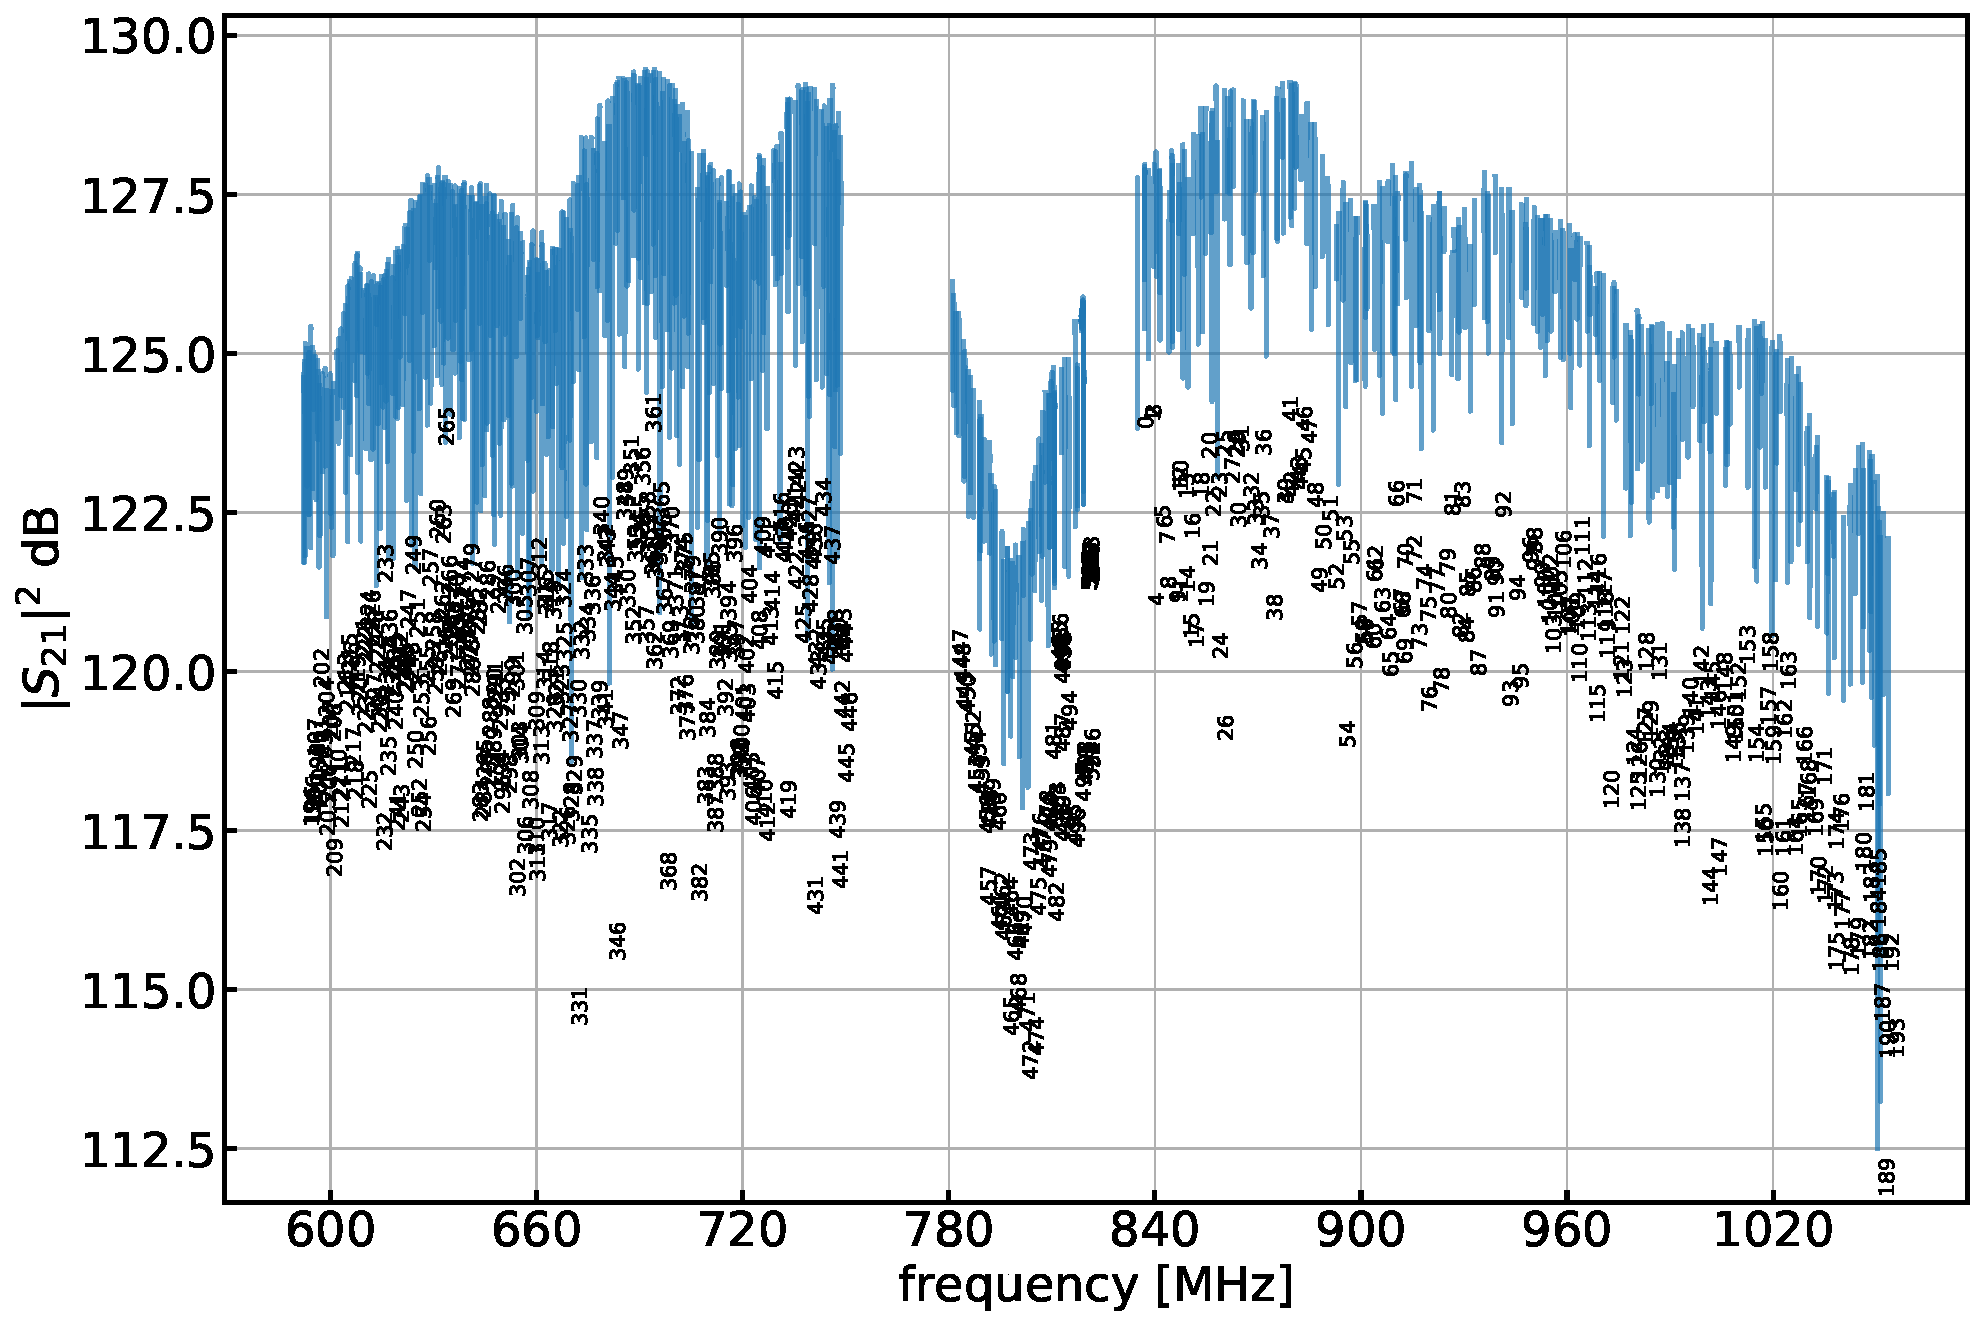
\includegraphics[width=\textwidth]{figures/blast_data/sweeps/350_targ_fts}
\caption[~An example \macrocapwrap{350~$\upmu$m} target sweep.]{An example 350~$\upmu$m target sweep.}
\label{fig:350 targ fts}
\end{figure}

\begin{figure}[!htbp]
\centering
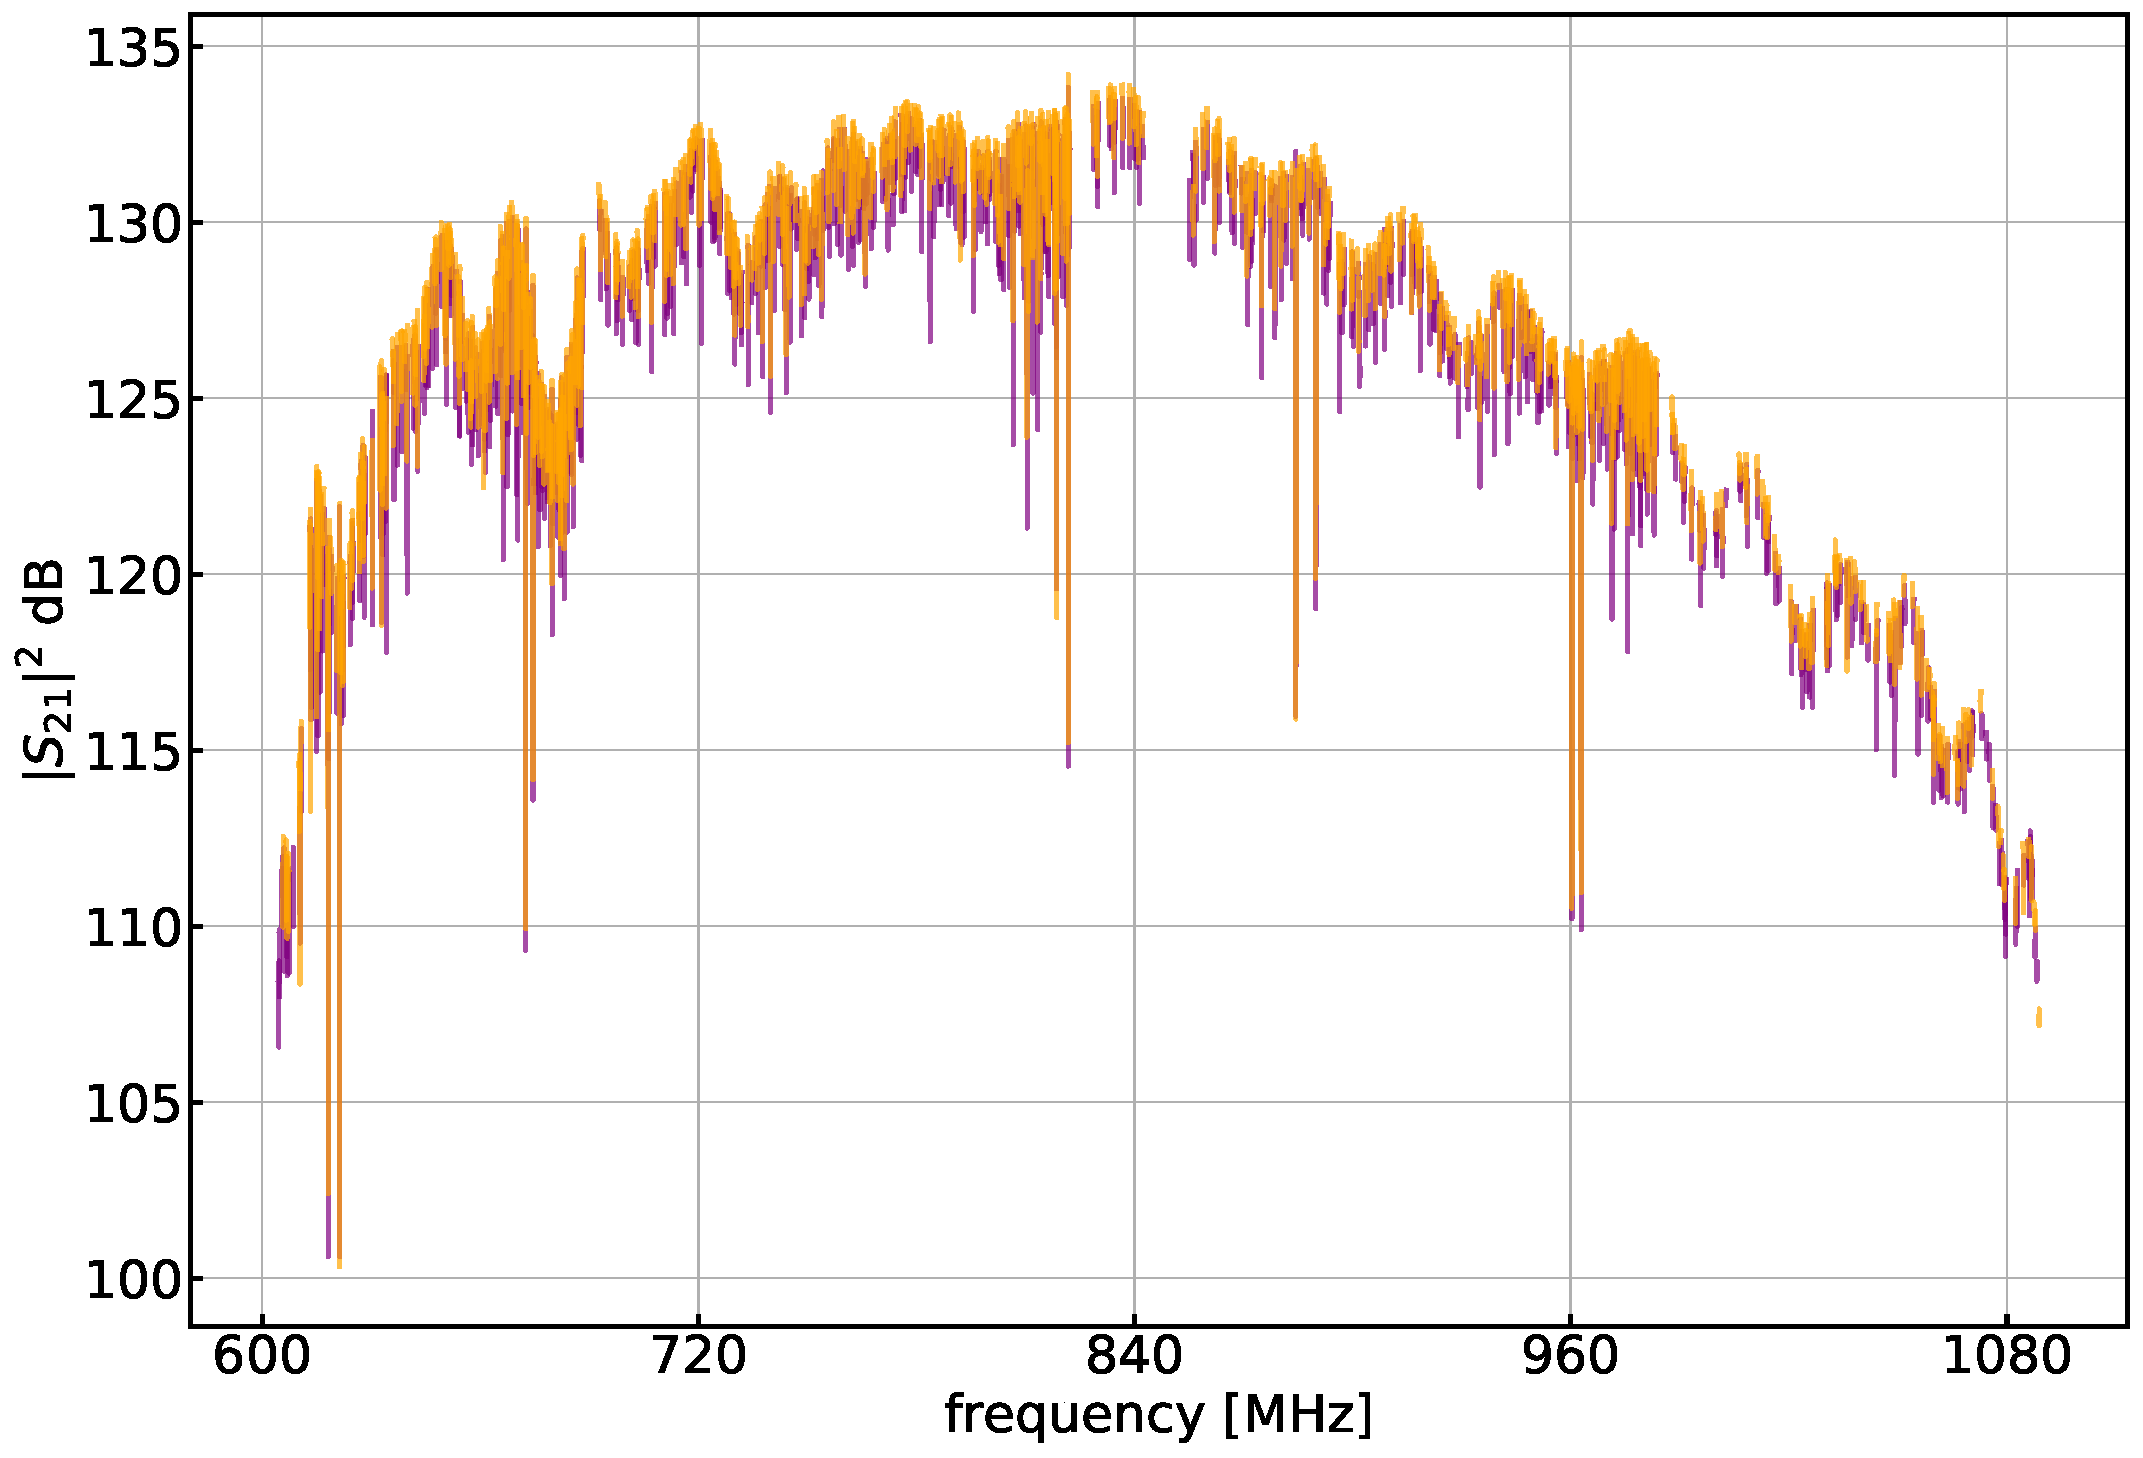
\includegraphics[width=\textwidth]{figures/blast_data/sweeps/350_targ_ice_overplot}
\caption[~\macrocapwrap{350~$\upmu$m} target sweeps from the ice, with shutter open and closed.]{350~$\upmu$m target sweeps from the ice, with shutter open (orange) and closed {purple}.}
\label{fig:350 targ ice}
\end{figure}

\subsection{Readout Power Optimization}\label{readout power}

The readout probe tones have an effect on resonator frequencies and quality factors. These effects, and their relation to the nonlinear kinetic inductance, are discussed in Chapter~\ref{kid_model}. Figures~\ref{fig:may out atten} and~\ref{fig:may out atten bifurc} show the effects of varying the readout power for two different resonators on one of the 250~$\upmu$m arrays. In this example, the readout power was increased in six increments of 3~dB by decreasing the warm output attenuation in the ROACH2 IF electronics, producing a range of tone powers from $\sim$ -90 to -72 dBm. The output attenuator settings, in dB, are listed in the figure legends.

The data shown in Figures~\ref{fig:may out atten} and~\ref{fig:may out atten bifurc} are overlays of target sweeps taken at each readout power. In each figure, the top panel shows $\left| \gls{S21} \right|^{2}$, the middle panel shows the phase of \gls{S21}, \gls{phiIQ}, and the bottom panel shows the $I/Q$ circle in the complex plane, in scaled raw units, for $\gls{S21}V_{\mathrm{readout}}$. It can be seen in both figures that above a certain readout power, the resonator frequency detuning and Q degradation becomes nonlinear (due to the nonlinear kinetic inductance). For both channels, the resonator detuning reaches $\sim$1~linewidth before the nonlinearity sets in. For the resonator in Figure~\ref{fig:may out atten bifurc}, bifurcation sets in before the last 6~dB of tone power stepping. The bifurcation is visible as a sharp discontinuity in each panel.

At lower readout powers, the effects seen in $\left| \gls{S21} \right|^{2}$, \gls{phiIQ} and in the $I/Q$ circle are similar to what would be observed from either optical or thermal loading. As tone power increases, the slope of the phase decreases, and the $I/Q$ circles become more elliptical.

In practice, the optical responsivity of each resonator is maximized at a slightly different readout power. As a rule of thumb, the optimal tone power can be set for each channel by first identifying that channel's bifurcation power, and then backing it off by $\sim$6~dB. The tone powers can also be optimized in a global sense, by adjusting the ROACH2 output attenuator while measuring the frequency noise on and off-resonance ($f_{0} + \sim$100~kHz). The on-resonance noise level is the sum of the LNA, detector and photon noise, whereas the off-resonance noise level reflects the LNA noise. Therefore, if the noise level on-resonance is greater than the off-resonance noise for a given channel, then the channel is assumed to be at least detector-noise limited. Above some attenuator setting, the vast majority of resonators should be biased in the detector-noise limited regime.

\begin{figure}[!ptbh]
\centering
\caption[~Sweeps at different tone powers for a single resonator.]{$\left| \gls{S21} \right|^{2}$, \gls{phiIQ} and $I/Q$ loops for target sweeps of a single 250~$\upmu$m channel for a range of warm output attenuator settings.}
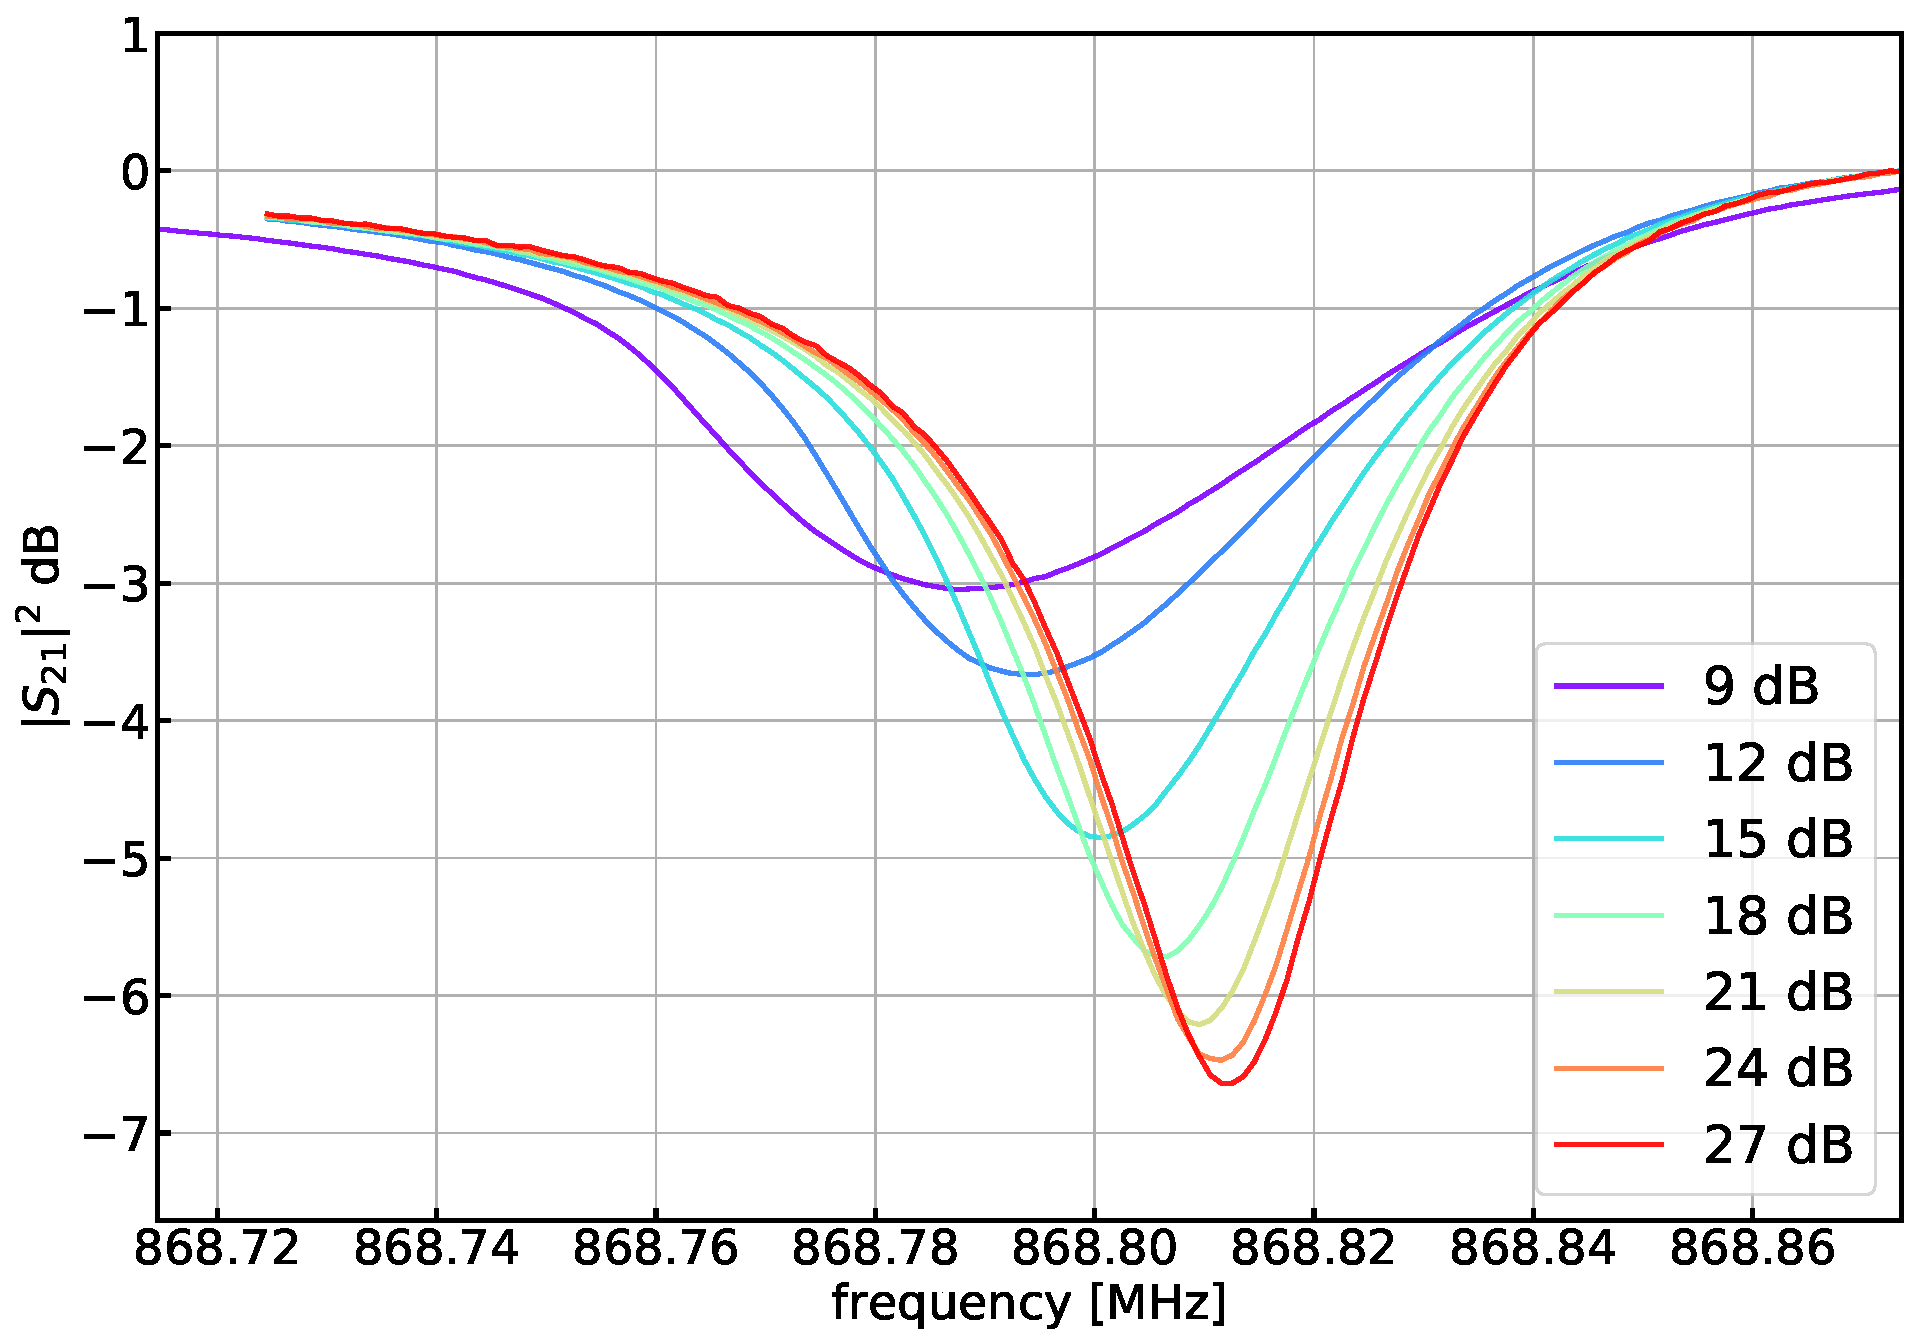
\includegraphics[width=0.68\textwidth]{figures/blast_data/sweeps/mag_tone_power_may}
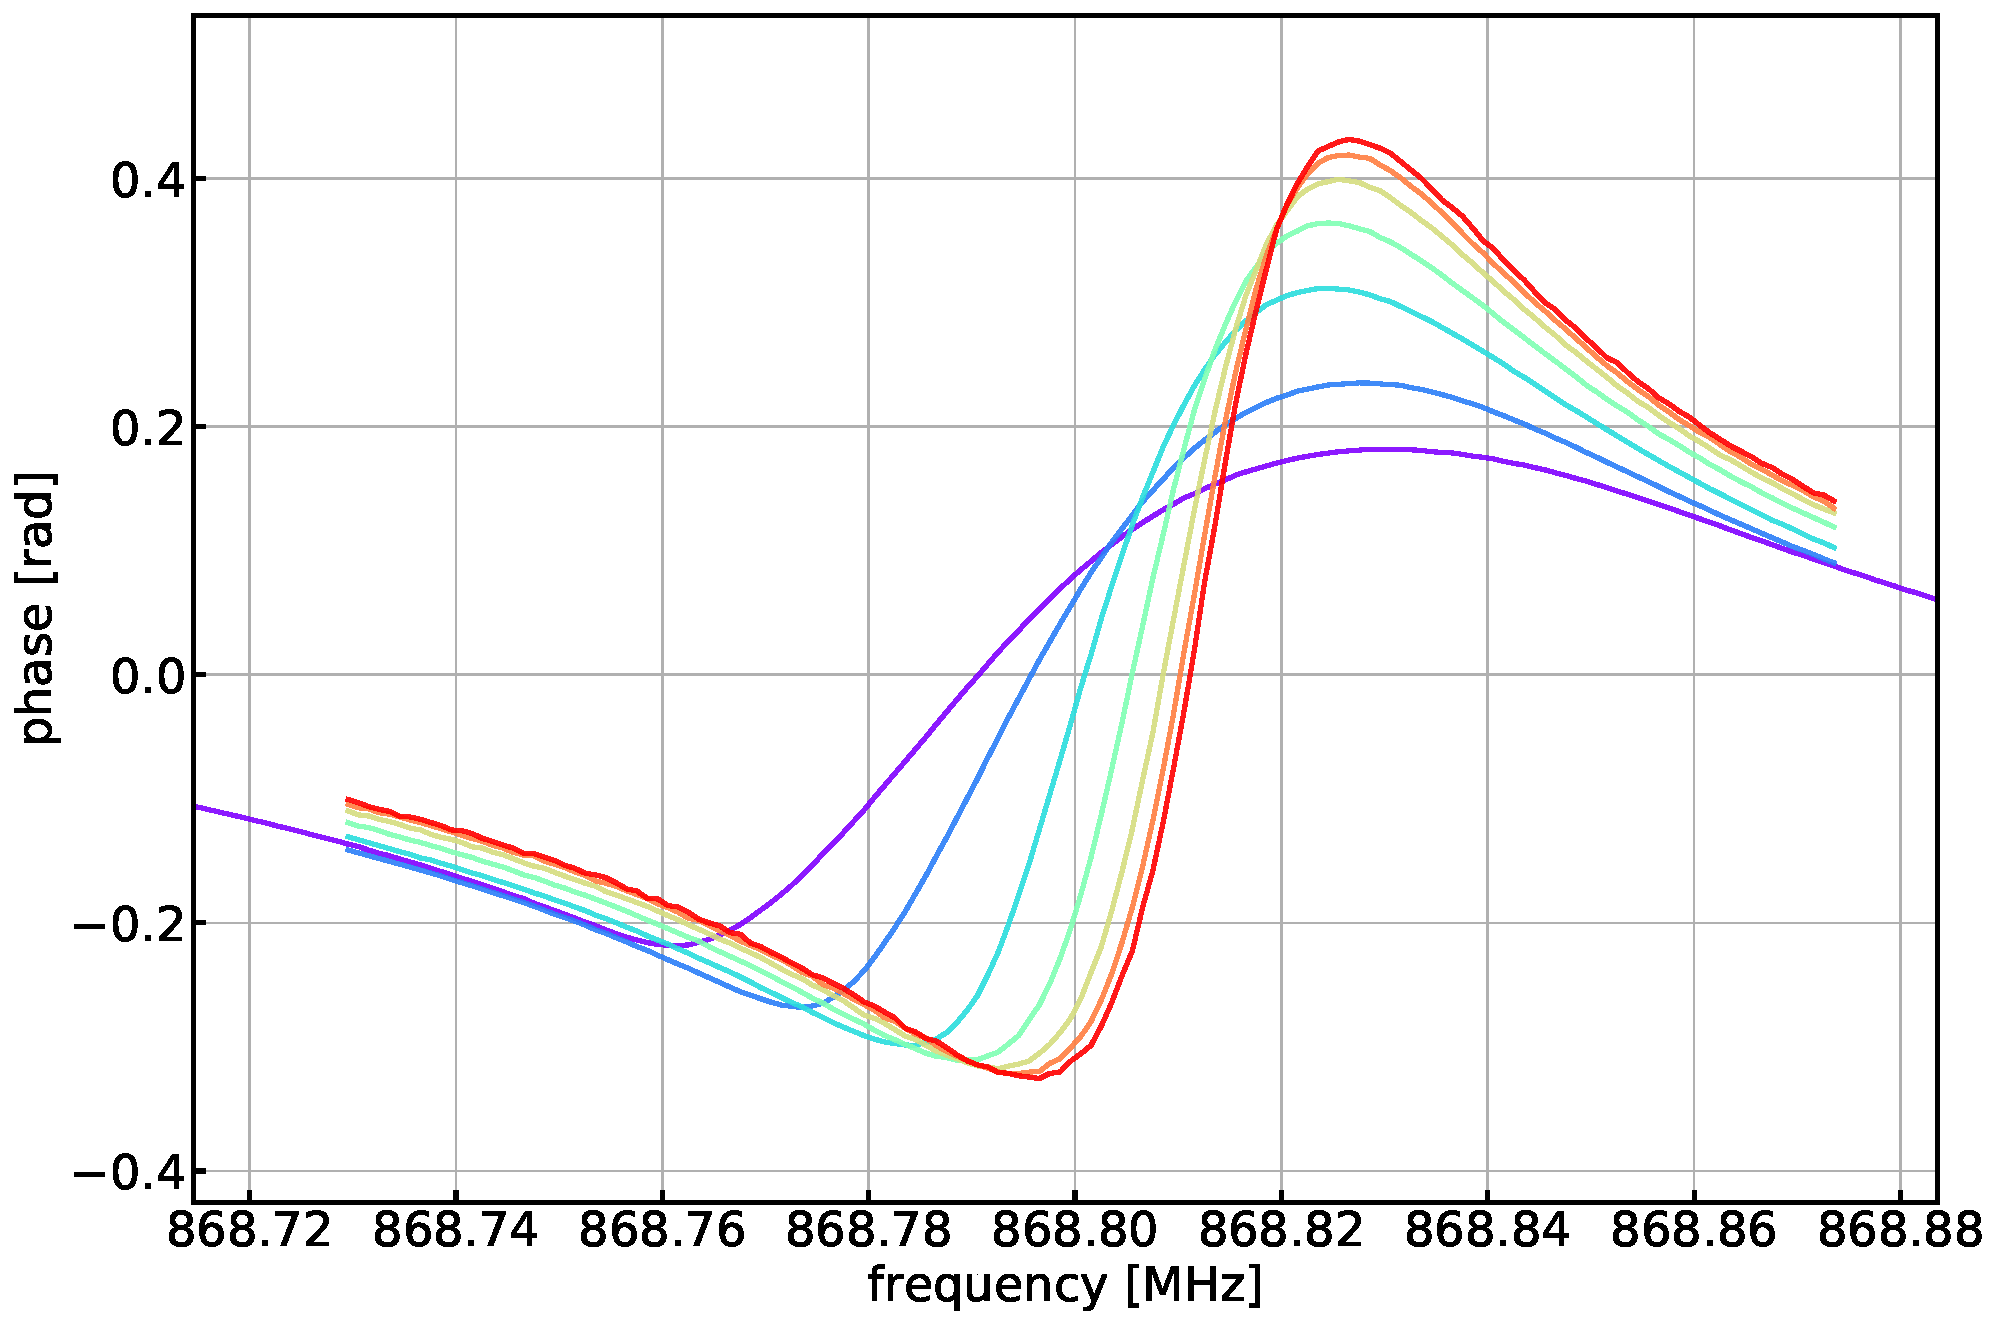
\includegraphics[width=0.68\textwidth]{figures/blast_data/sweeps/phase_tone_power_may}
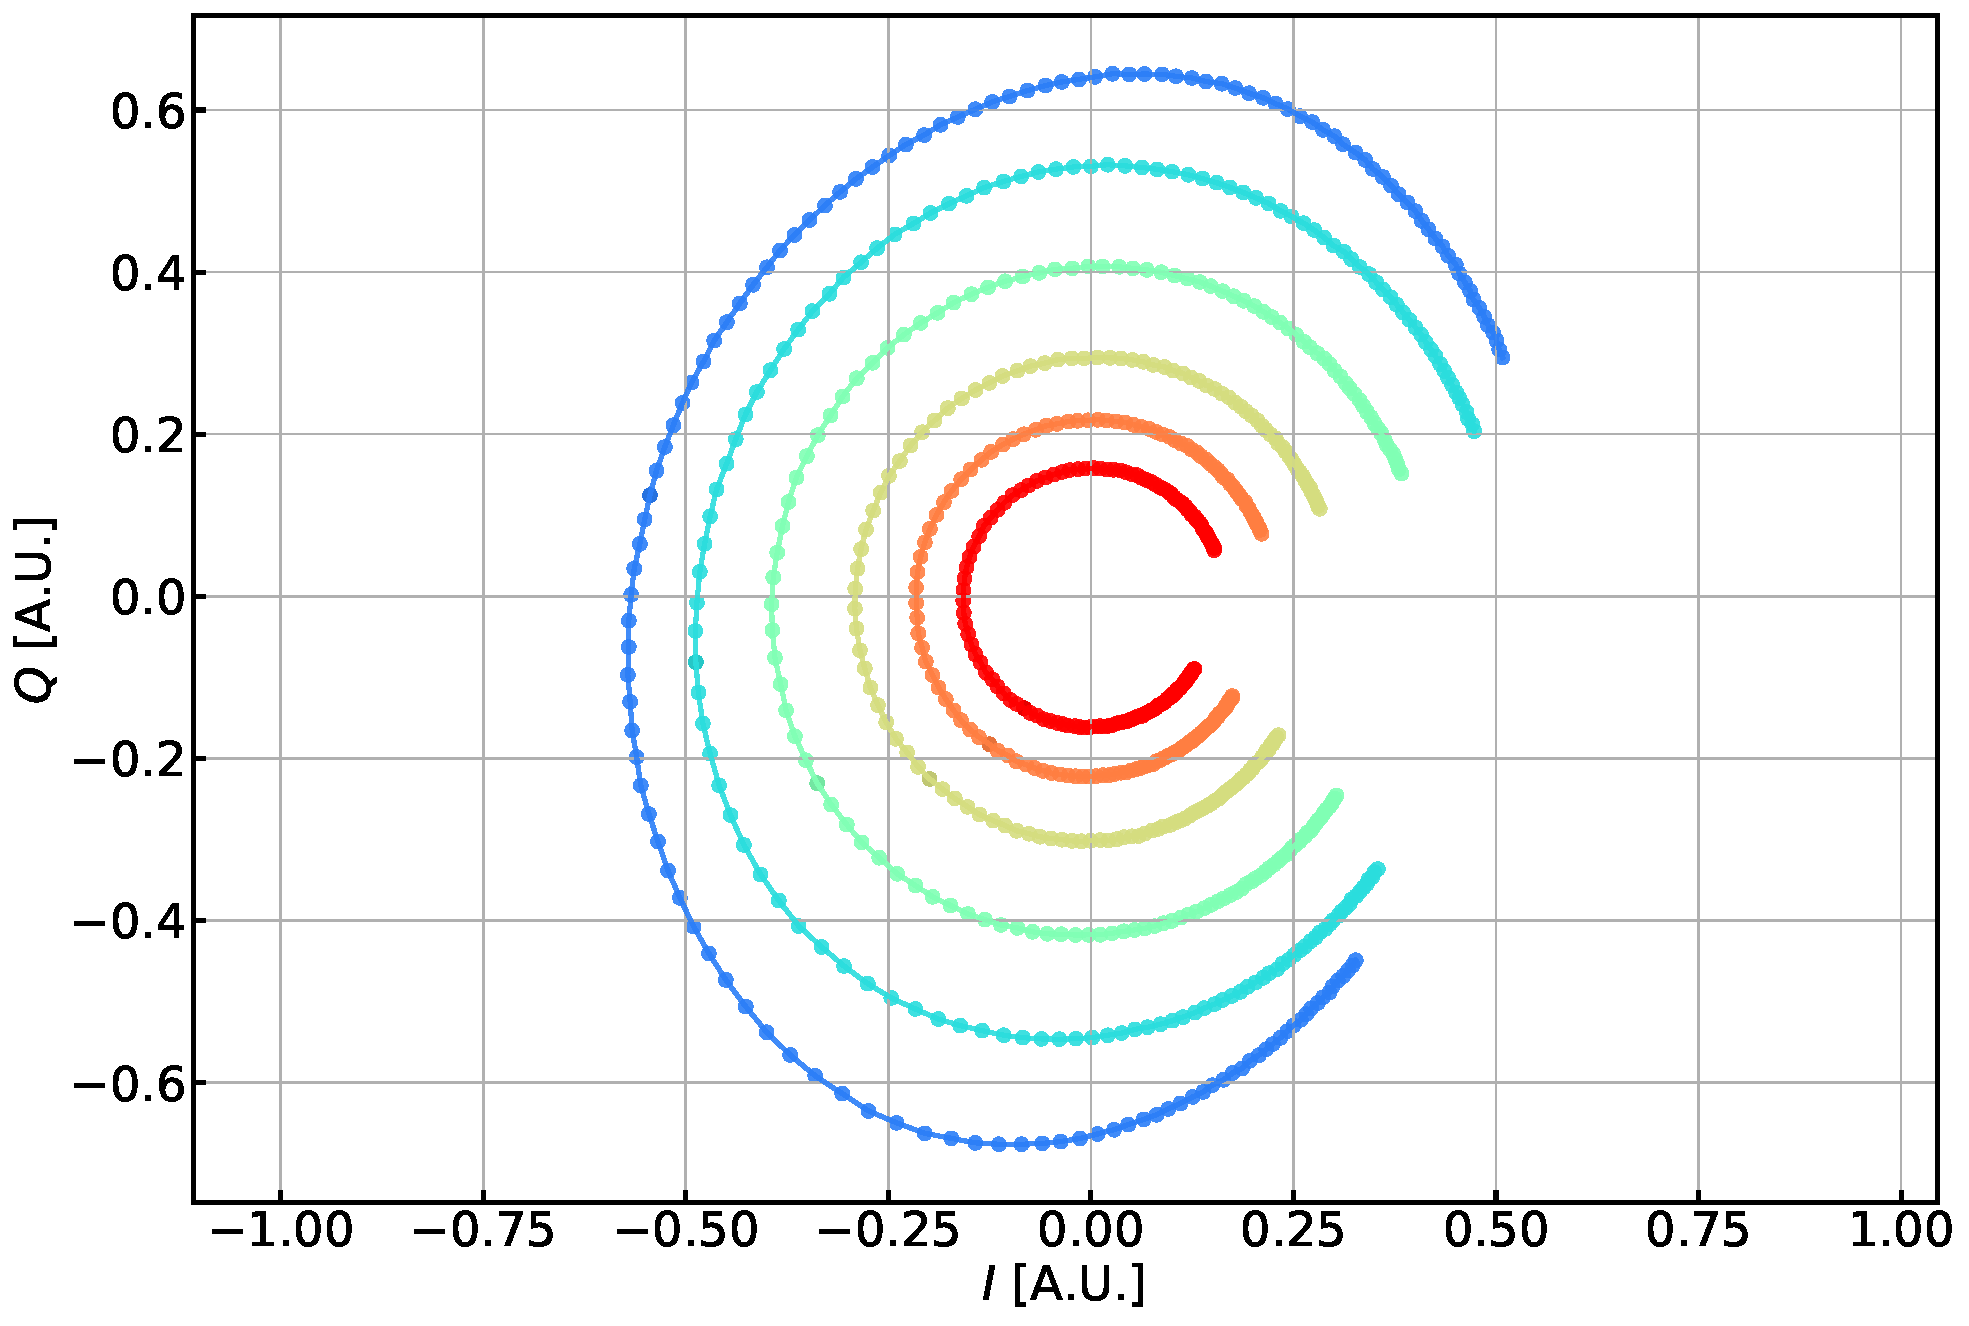
\includegraphics[width=0.68\textwidth]{figures/blast_data/sweeps/IQ_tone_power_may}
\label{fig:may out atten}
\end{figure}

\begin{figure}[!ptbh]
\centering
\caption[~Sweeps at different tone powers for a single resonator, showing bifurcation.]{$\left| \gls{S21} \right|^{2}$, \gls{phiIQ} and $I/Q$ loops for a range of warm output attenuator settings, showing bifurcation.}
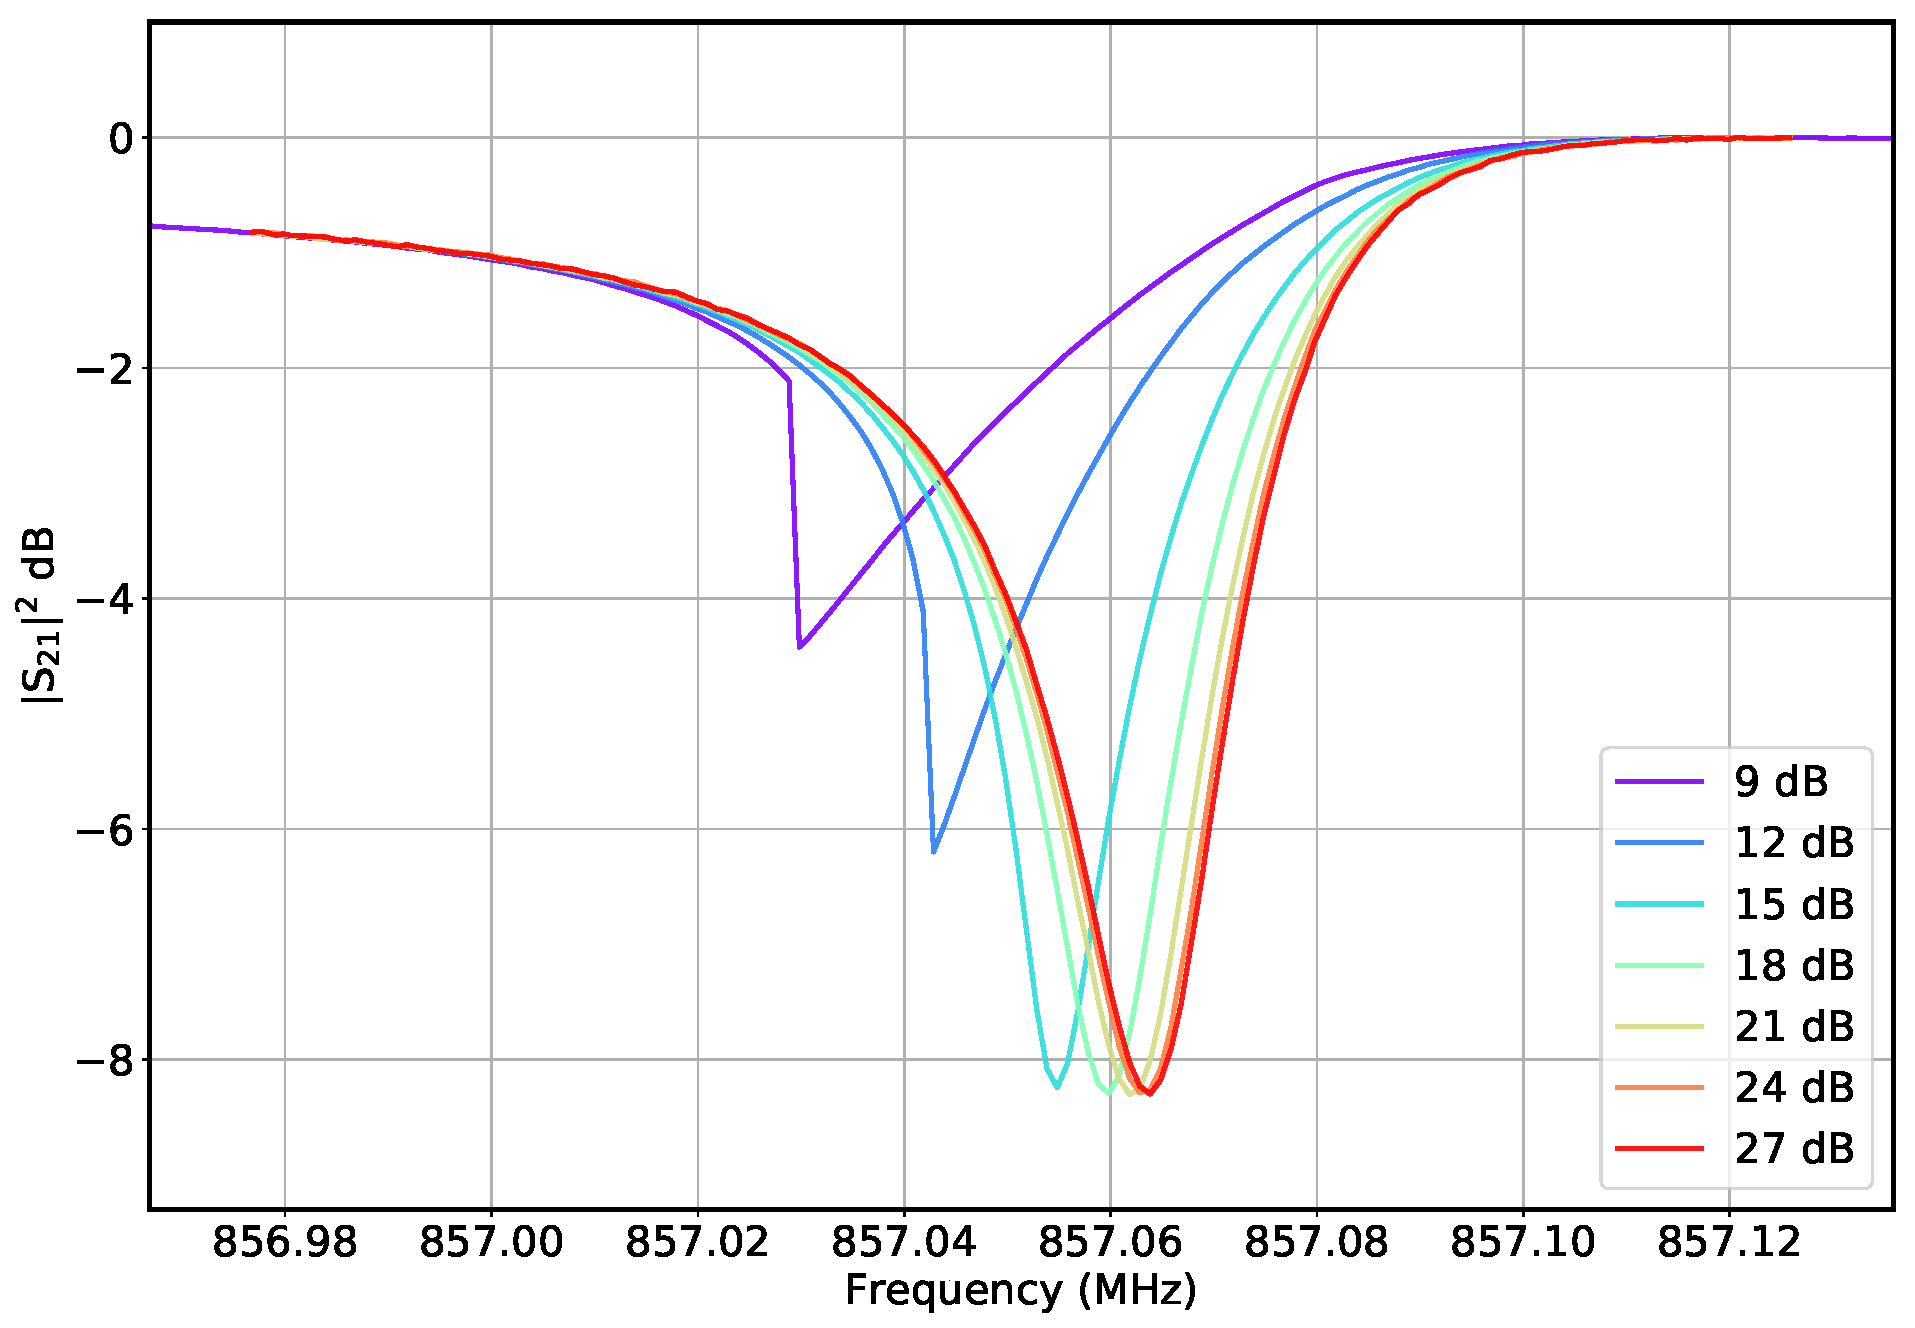
\includegraphics[width=0.68\textwidth]{figures/blast_data/sweeps/mag_tone_power_bifurc}
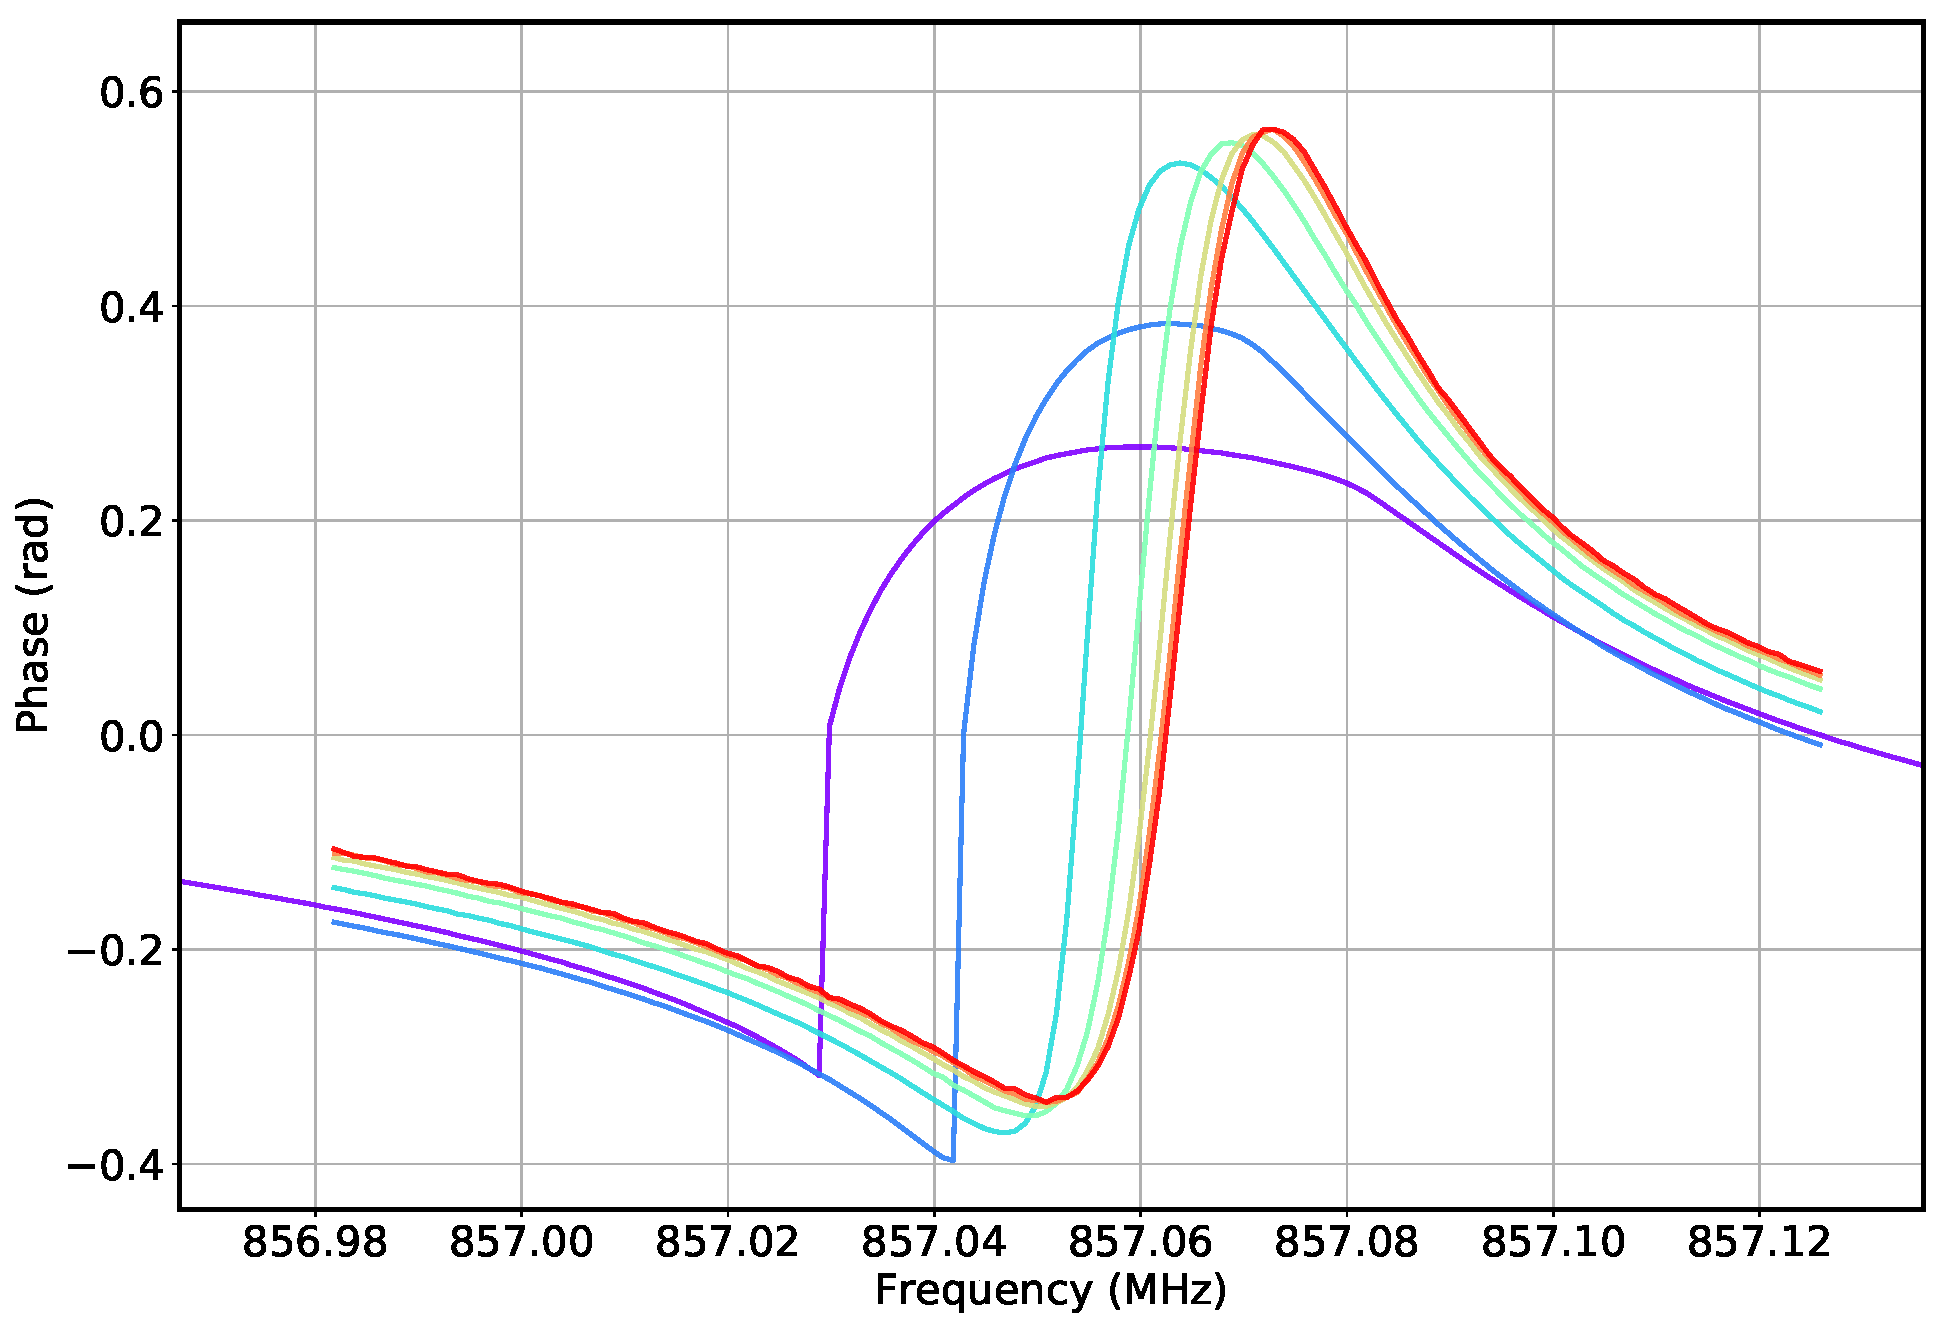
\includegraphics[width=0.68\textwidth]{figures/blast_data/sweeps/phase_tone_power_bifurc}
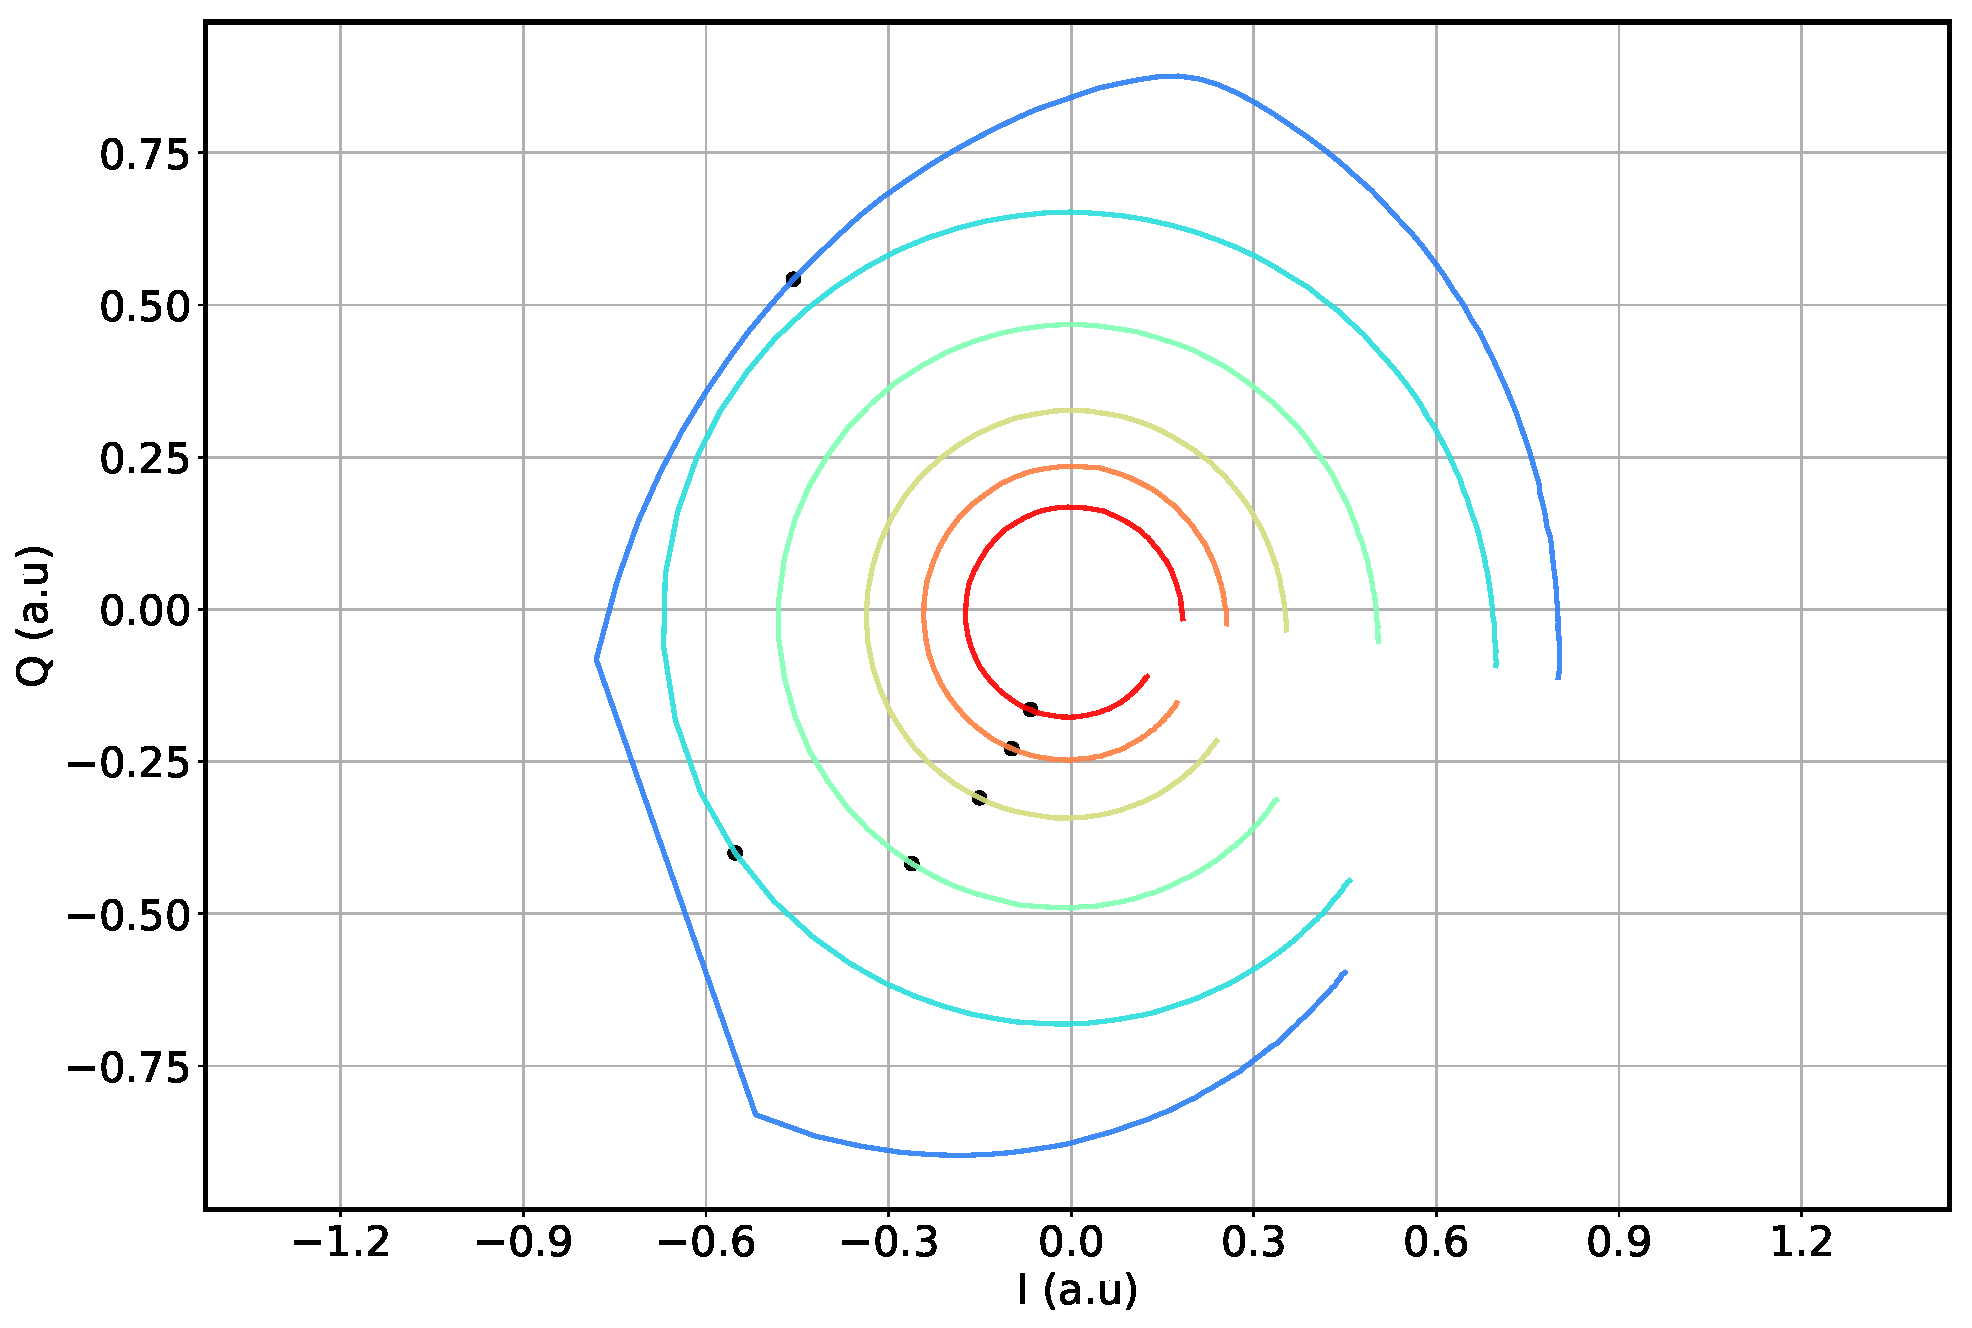
\includegraphics[width=0.68\textwidth]{figures/blast_data/sweeps/IQ_tone_power_bifurc}
\label{fig:may out atten bifurc}
\end{figure}

\section{Detector Timestreams}\label{timestreams}

The readout outputs two 32-bit samples, $I[n]$ and $Q[n]$, for each channel at a rate of 488.28125~Hz (once every $\approx$~2~ms). $I$ and $Q$ represent the demodulated channel amplitude: $\gls{S21}[n] = I[n] +jQ[n] $. With knowledge of the readout processing gain, it would be possible to convert $I$ and $Q$ into absolute units of volts. However, because it is \gls{phiIQ} which is proportional to the absorbed optical power, it is not necessary to perform this calibration. $I$ and $Q$ are therefore saved to disk in raw units, and then used to calculate the frequency shift of the resonator for each sample, \gls{df} (which is proportional to the phase shift of the probe tone). This process is described in the following section.

\subsection{Converting \macrocapwrap{$I/Q$} to \macrocapwrap{\gls{df}}}\label{df calc}

In the following, we describe the steps of the data reduction which are taken to convert the $I/Q$ timestreams to units of frequency shift, \gls{df}, relative to the resonant frequency of each channel. If the frequency responsivity is known, the system NEP can be calculated by measuring the frequency noise $(e_{f}/f_{0})^{2} = \gls{Sxx} = \gls{Sff}$ $[\mathrm{Hz}^{-1}]$ (see Section~\ref{sensitivity}).

To convert $I/Q$ to units of frequency requires either a recent target (or wide) sweep of the resonator. Hereafter, this sweep is referred to as the reference sweep. Two methods of converting \gls{S21} to frequency units are commonly used. These are the $I/Q$ gradient (\gls{gradIQ}) and the phase-fitting method. The relative advantages of each method are described in detail in \citet{barry2014development}. Choosing between the two methods entails a trade-off between computational efficiency and accurate representation of the frequency shift. The gradient method is more computationally efficient than the phase method at the expense of not accounting for the change in the shape of the resonant circle when $f_{0}$ is shifted far from resonance (more below). Ultimately, the gradient method underestimates the frequency noise by a factor of $\sim$1.5 \citep{barry2014development}.

For real-time estimates of \gls{df} during a measurement, we find that the $I/Q$ gradient method is preferred over the phase-fitting method. The gradient method is described in detail in \citet{d2013nika} (for a description of the phase method, see \citet{gao2008physics}). Here, we summarize its key elements. Using the reference frequency sweep, \gls{df} (in the continuous time domain) is calculated from \gls{S21} as:

% df
\begin{equation}\label{eq:df1}
   \delta f(t) = \frac{\delta \gls{S21}}{\nabla_{f}\gls{S21}} = \frac{\delta I(t) + j\delta Q(t)}{\nabla_{I,Q}}
\end{equation}

Rationalizing Equation~\ref{eq:df1} yields:

\begin{equation}\label{eq:df2}
    \delta f(t) = \frac{\delta I(t) \cdot dI/df + \delta Q(t) \cdot dQ/df}{(df/dQ)^{2} + (dQ/df)^{2}} - j\frac{\delta I(t) \cdot dQ/df - \delta Q(t) \cdot dI/df}{(df/dQ)^{2} + (dQ/df)^{2}}
\end{equation}

where all of the $I/Q$ values are with respect to the resonant frequency, $\delta I(t) = I(t) - I_{\mathrm{ref}}$ and $I_{\mathrm{ref}}$ ($Q_{\mathrm{ref}}$) are the $I/Q$ values on resonance at the time at which the reference sweep was taken. The \gls{df} values produced by this method are valid only if the resonator has shifted by less than a linewidth (see below). Figure~\ref{fig:IQ grad} shows an example \gls{gradIQ} calculation for one channel (channel 448) of the 350~$\upmu$m array. The value of \gls{gradIQ} which is used in Equations~\ref{eq:df1} and~\ref{eq:df2} is taken where $\left| \gls{gradIQ} \right|$ at its maximum. This point is marked with the dotted black line in Figure~\ref{fig:IQ grad}.

In practice, SNR variations in the target sweeps translate into errors in the \gls{gradIQ} calculation. During a measurement, it is possible to calibrate \gls{gradIQ} by chopping the LO in frequency by a fixed amount both above and below the center frequency. If the probe tone is perfectly centered on the resonant frequency, and \gls{Qr} is moderately high, the \gls{df} step observed in the timestreams for each channel should equal the chop \gls{df}. If the probe tone is within a resonator linewidth of $f_{0}$, but off-center relative to $f_{0}$, the \gls{df} observed in the timestreams will be asymmetric. If the probe tone is too far out of range of $f_{0}$, the LO chop will have little to no observable effect in the channel timestreams.

If the probe tone is known to be on or very near resonance, the LO chop provides a good indicator of the accuracy of the \gls{gradIQ} values. During the BLAST-TNG flight the LO chop will performed during each azimuth turnaround (the data acquired during these turnaround will not be used to make science maps). The \gls{df} chops which are imprinted into each channel's timestream can be used to calibrate the $I/Q$ data post-flight.

Figure~\ref{fig:lo chops} shows an example LO chop for one channel from the 250U, 350 and 500~$\upmu$m arrays, taken during pre-flight preparations at LDB\@. The frequency step-size is 2.5~kHz for the 250 and 350~$\upmu$m arrays, and 10~kHz for the 500~$\upmu$m. At the time when these LO chops were recorded, the probe tones were very close to $f_{0}$, and the channel \gls{df} values match the LO chop. The spikes in the data located around the frequency jumps are due to drop-outs in the LO signal when the synthesizer is stepped.

% LO chops ICE
\begin{figure}[!htbp]
\centering
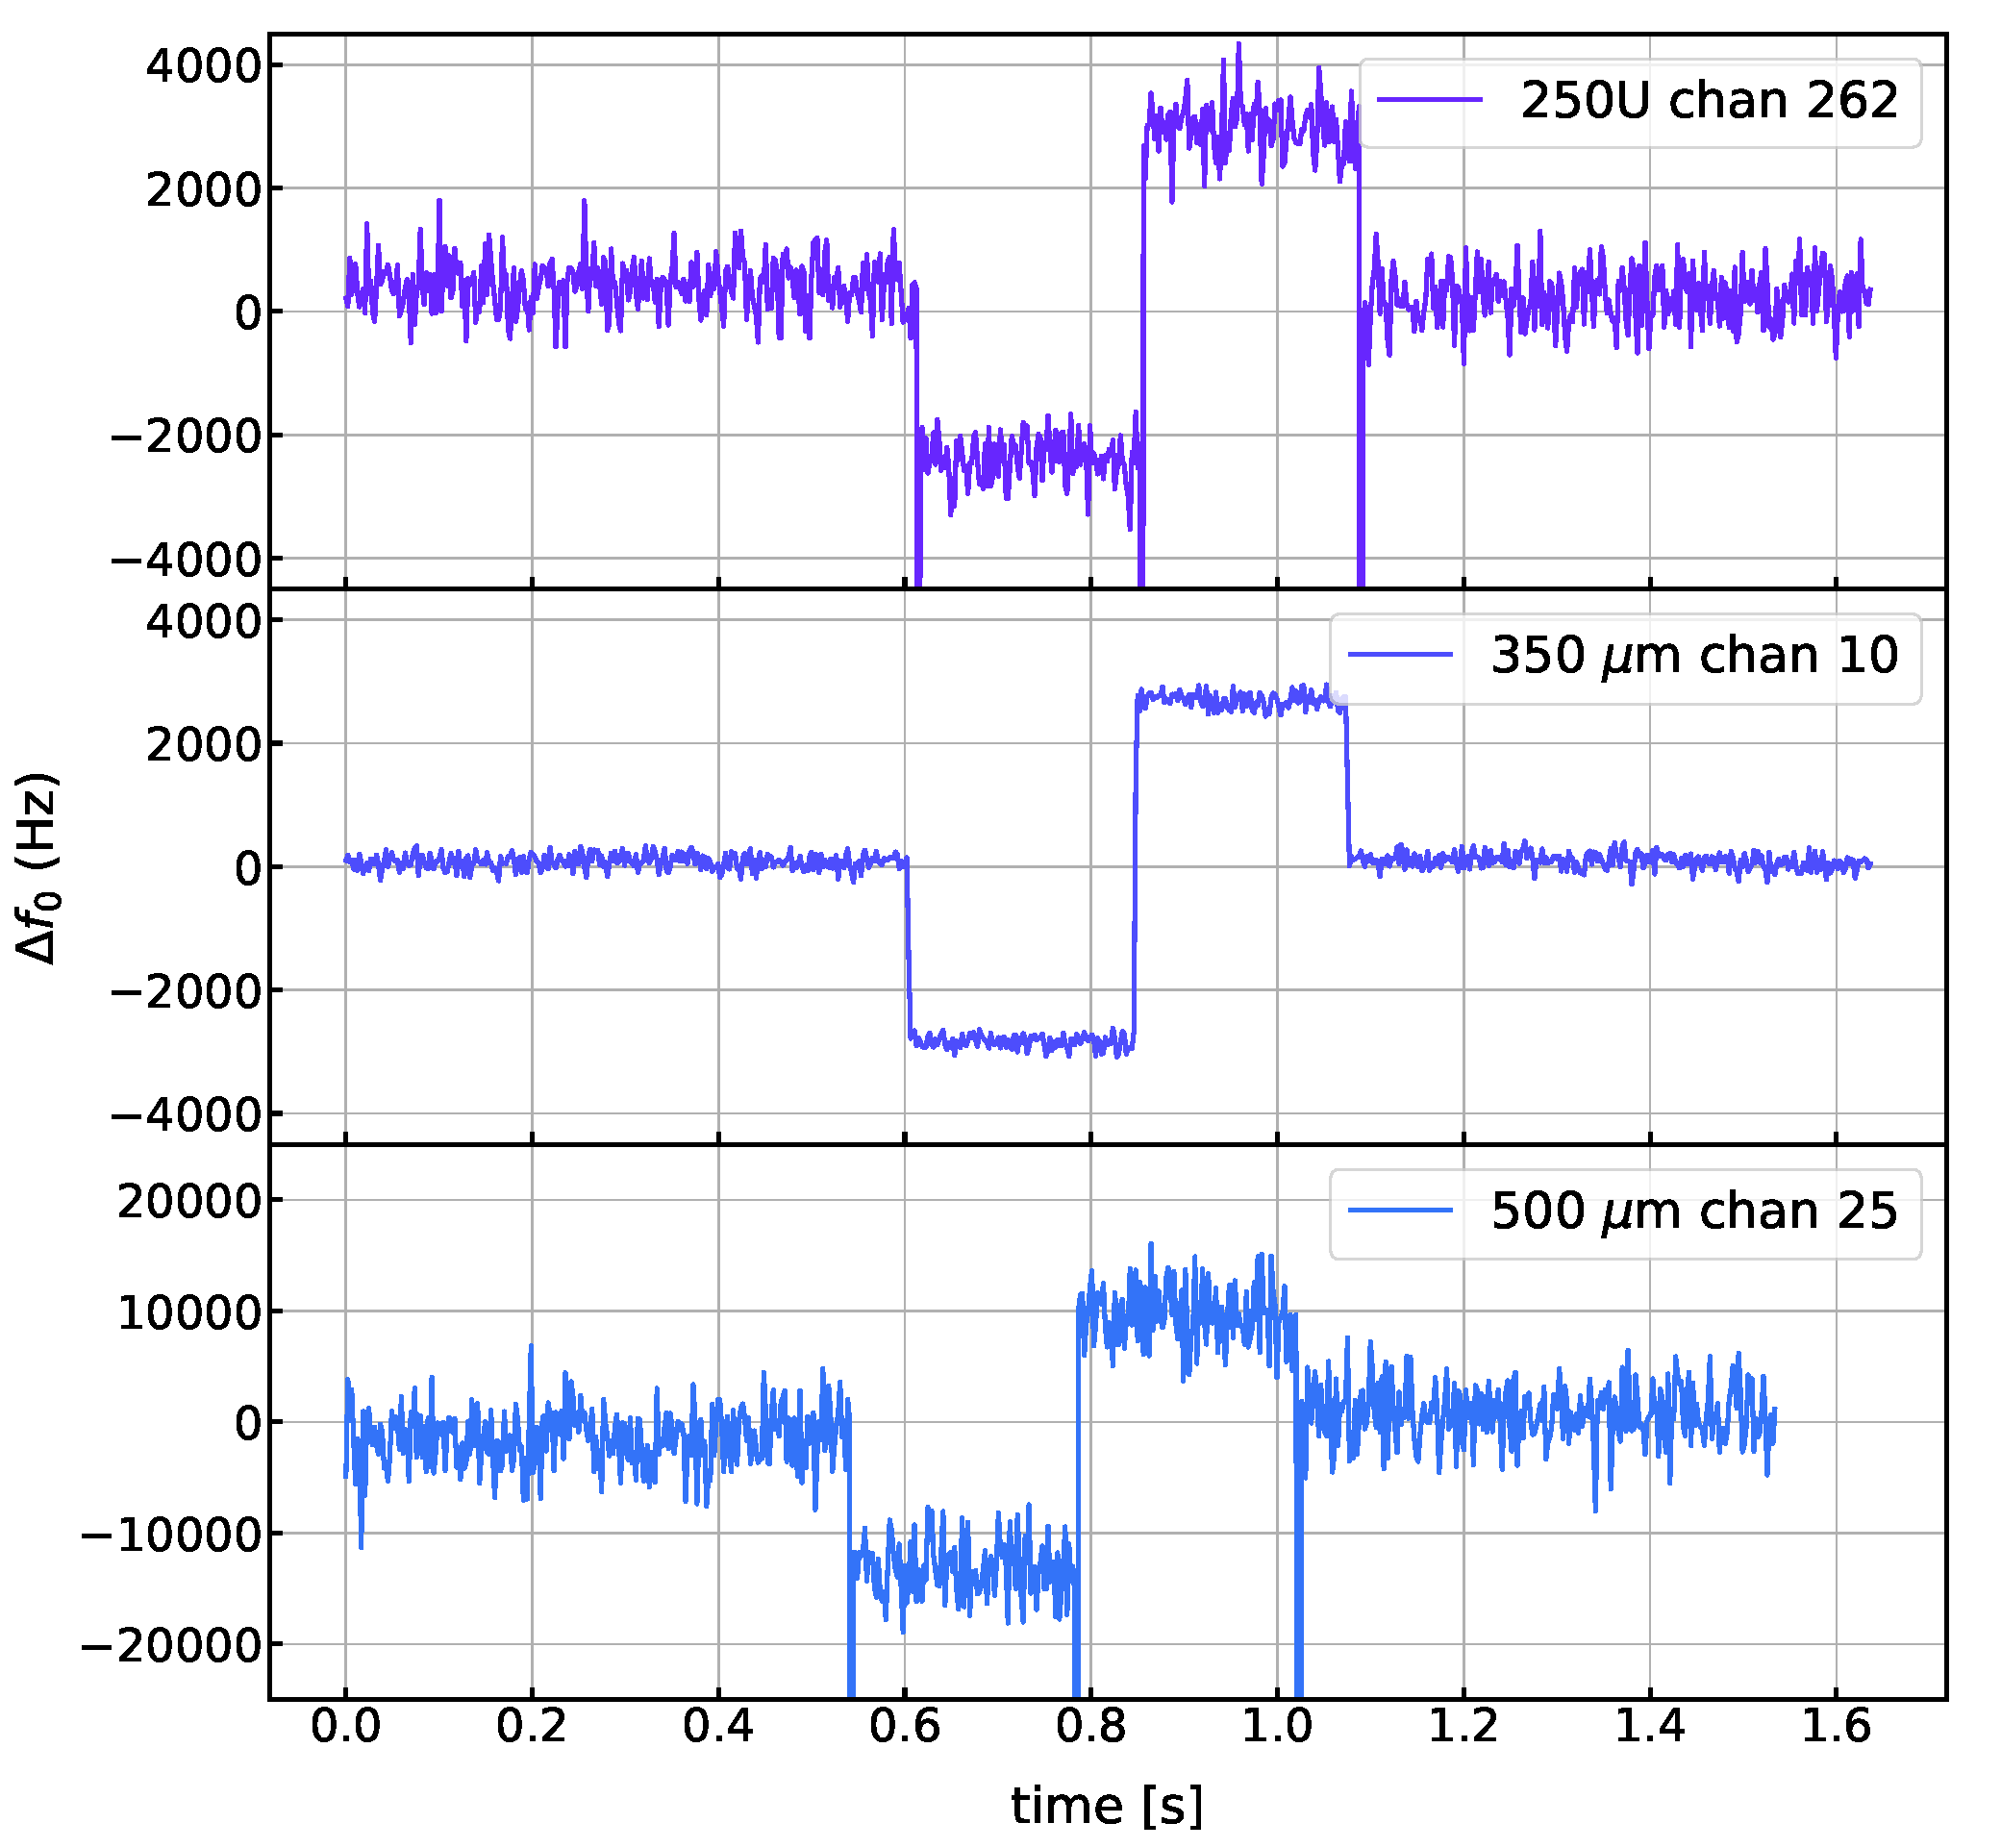
\includegraphics[width=\textwidth]{figures/blast_data/timestreams/ice_lo_chops}
\caption[~LO chops for the 250U, 350 and 500~\macrocapwrap{$\upmu$m} arrays.]{LO chops for the 250U, 350 and 500~$\upmu$m arrays.}
\label{fig:lo chops}
\end{figure}

\subsection{Phase and Dissipation Quadratures}

In Equation~\ref{eq:df2}, the real part of \gls{df}, $\Re(\gls{df})$, represents the total frequency fluctuation in the phase quadrature (tangent to the $I/Q$ circle in the complex-plane), and the imaginary part of \gls{df}, $\Im(\gls{df})$, represents the fluctuation in the dissipation quadrature (orthogonal to the $I/Q$ circle). The noise in the dissipation quadrature is primarily from the LNA (($e_{f,\mathrm{diss}}/f_{0})^{2} = \gls{Syy}$). The noise in the phase quadrature which is not due to the amplifiers can be estimated as $\gls{Sxx} - \gls{Syy}$. If the detectors are photon noise limited, then $S_{\mathrm{phot}} \simeq \gls{Sxx} - \gls{Syy}$. In the photon noise limited regime, \gls{Sxx} should be greater than \gls{Syy}.

Figure~\ref{fig:timestreams} shows a 10~s timestream for channel 448 of the 350~$\upmu$m array, recorded at CSBF\@. The timestream is shown as $I$ (top, raw units), $Q$ (second from top, raw units), $\Re(\gls{df})$ (second from bottom, Hz) and $\Im(\gls{df})$ (bottom, Hz). Figure~\ref{fig:example chan} shows $\left| \gls{S21} \right|^{2}$ (top), \gls{phiIQ} (middle) and the $I/Q$ circle for the example channel. The dashed red line in $\left| \gls{S21} \right|^{2}$ is a fit to the data which has been used to estimate the resonator parameters listed in Table~\ref{table:350 example chan}. The estimated parameters are: $f_{0}$, dip-depth, \gls{Qr}, \gls{Qc}, \gls{Qi}, \gls{asym} and \gls{Sff}. 10 seconds of timestream values are shown as a scatter ball (orange) in the phase and $I/Q$ circle panels. To plot \gls{phiIQ} and the $I/Q$ circle, the $I/Q$ values have been rotated so that the minimum value of $I$ coincides with the resonance point. This rotation prevents phase wrapping when plotting \gls{phiIQ}, and is achieved by multiplying \gls{S21} by a complex exponential, where

% Rotating I and Q
\begin{equation}
  S_{21,rot} = \gls{S21} e^{j\phi_{rot}}
\end{equation}

and $\phi_{rot} = \arctan2(\left< Q(t) \right>, \left< I(t) \right>)$.

% IQ grad
\begin{figure}[!htbp]
\centering
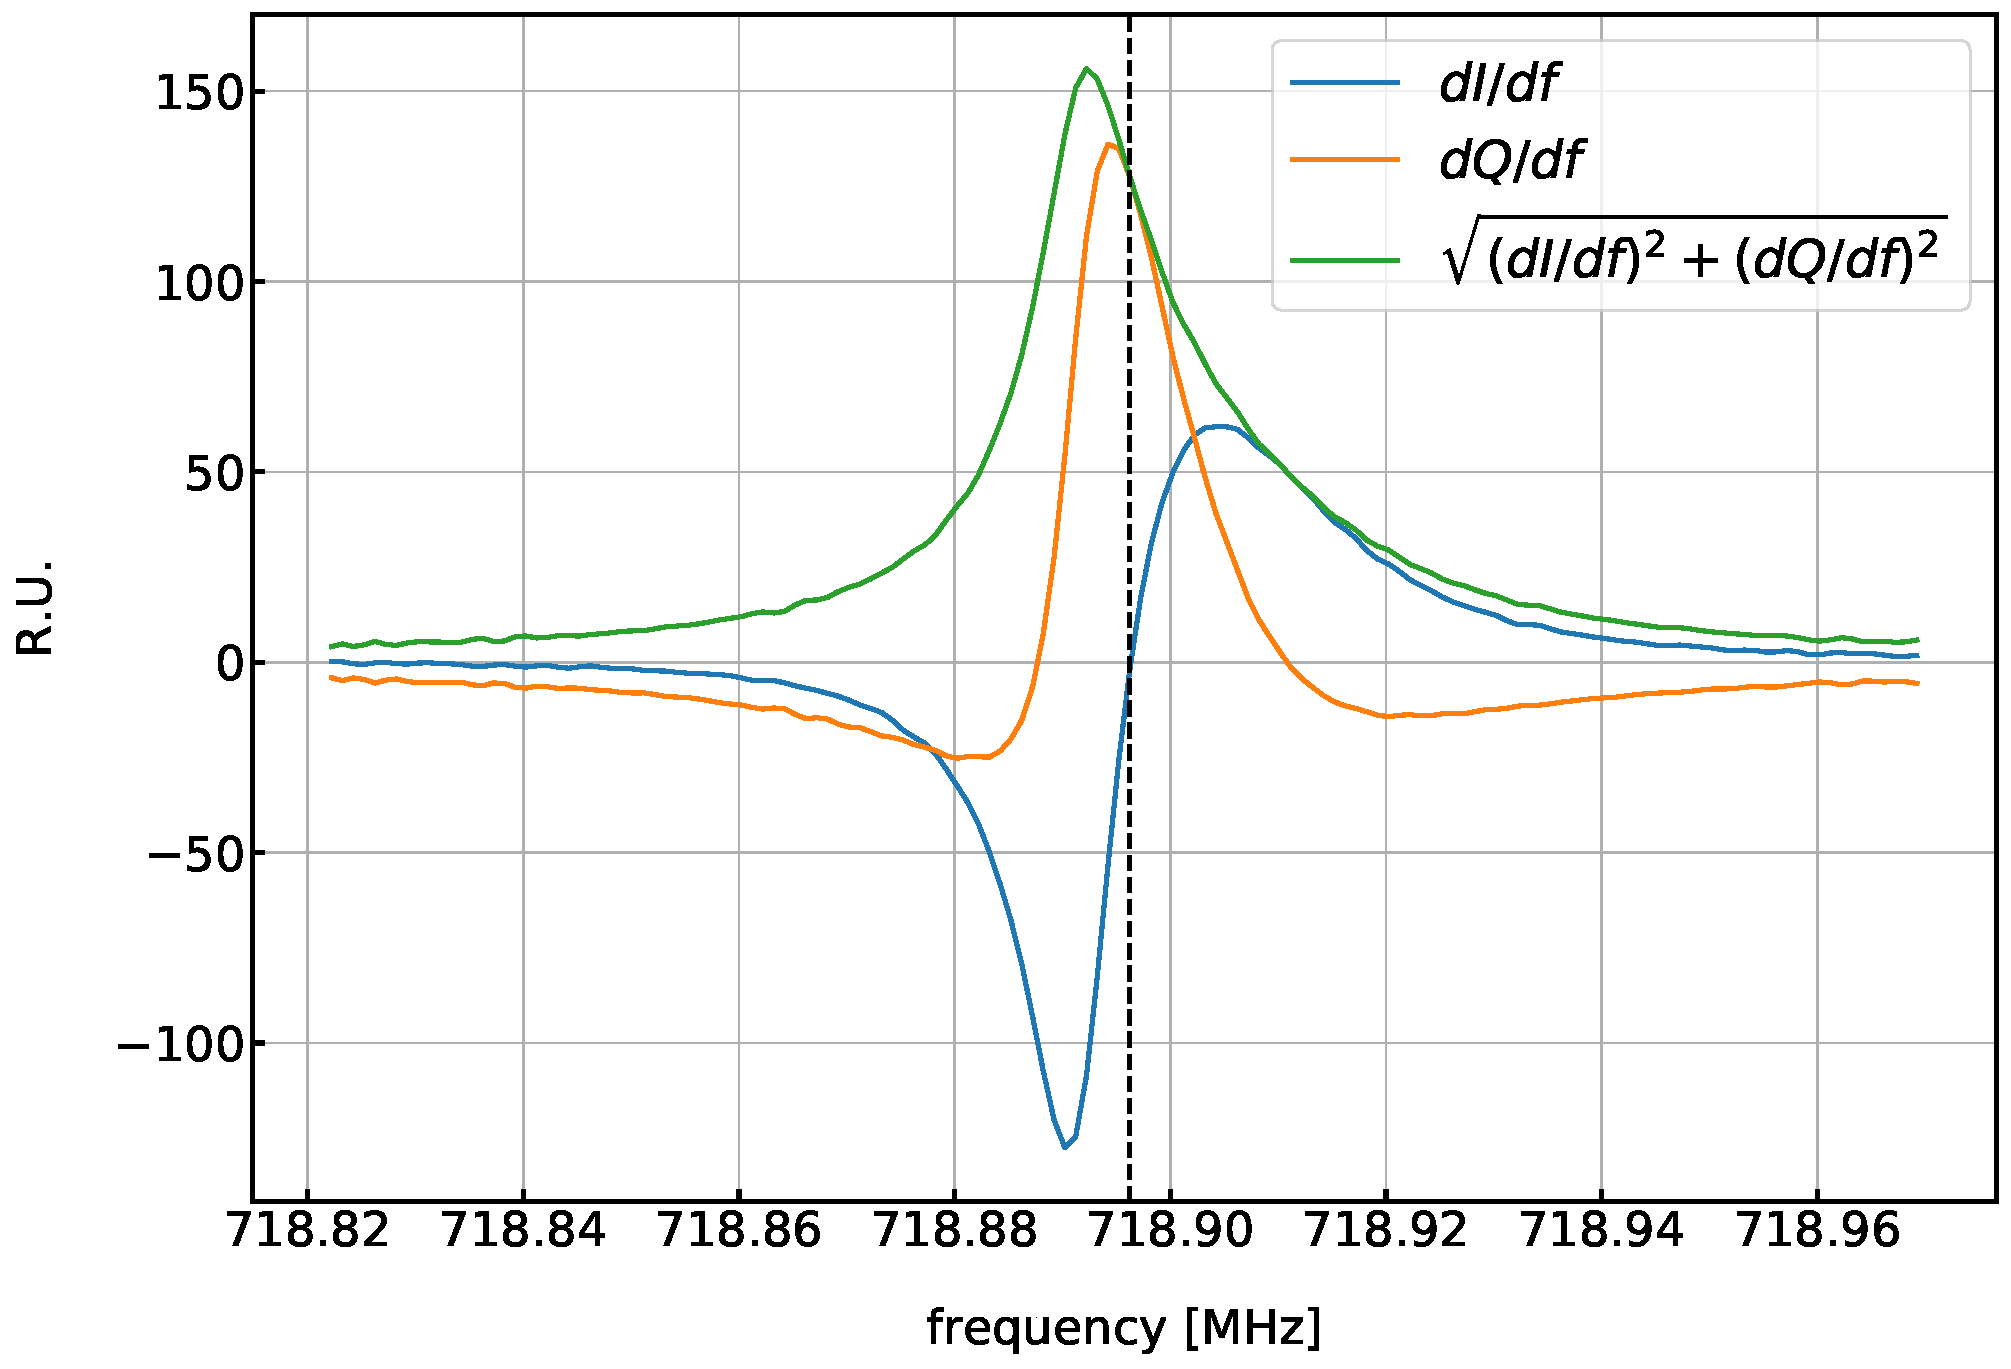
\includegraphics[width=\textwidth]{figures/blast_data/timestreams/350_pal_IQgradExample_448}
\caption[~\macrocapwrap{\gls{gradIQ}} for a single 350~\macrocapwrap{$\upmu$m} channel.]{An example of the $I/Q$ gradient \gls{gradIQ} calculation for a single 350~$\upmu$m channel.}
\label{fig:IQ grad}
\end{figure}

% Example chan timestreams
\begin{figure}[!htbp]
\centering
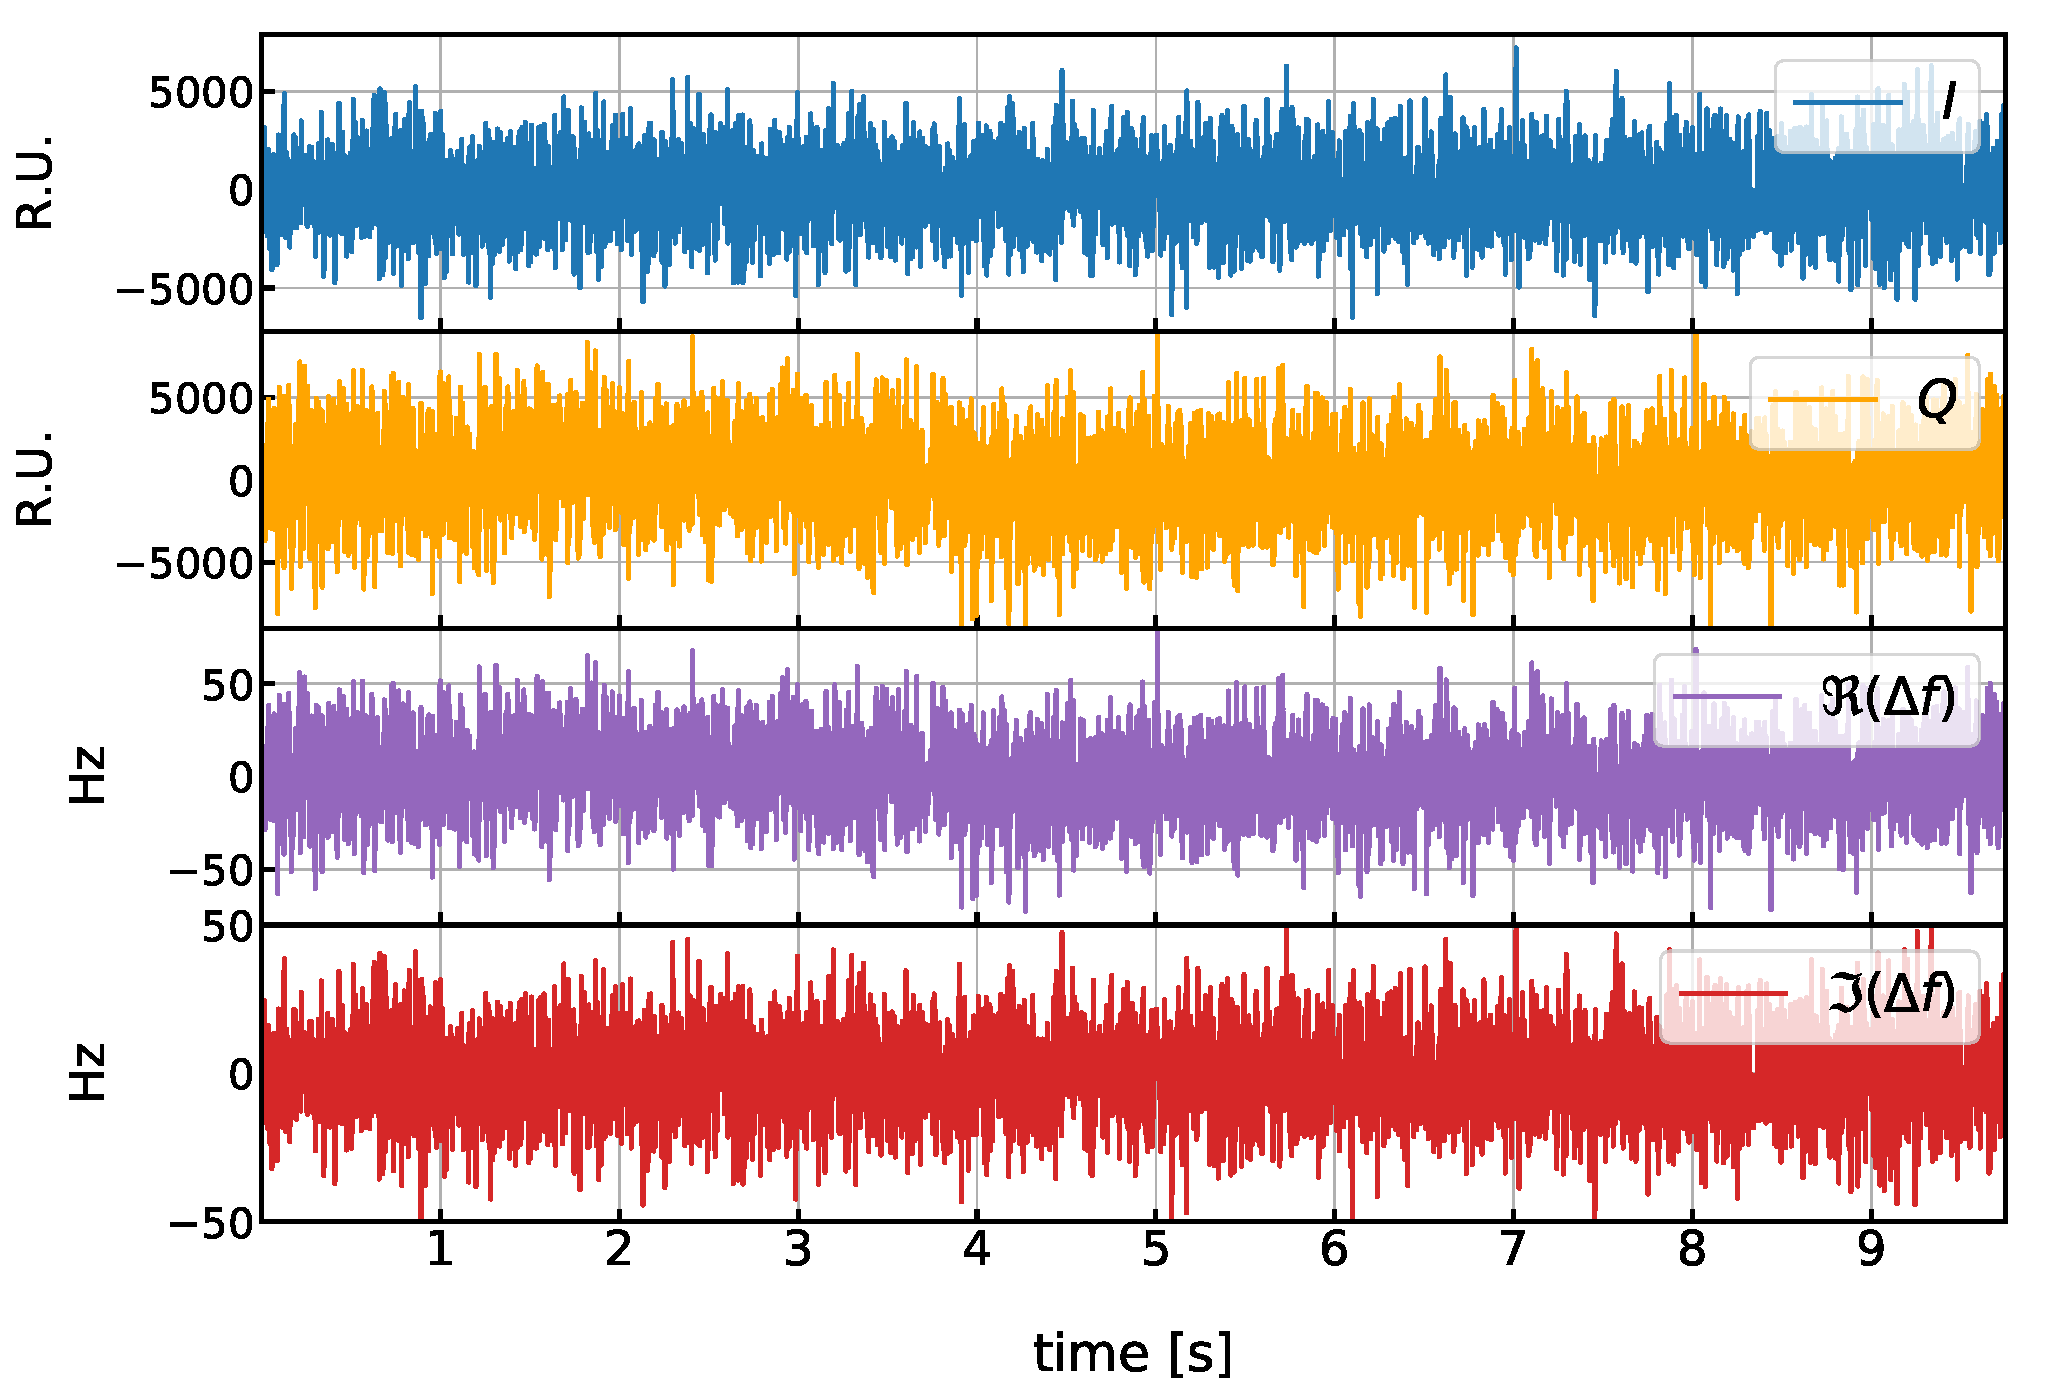
\includegraphics[width=\textwidth]{figures/blast_data/timestreams/350_pal_ts_and_df_448}
\caption[~10 second timestreams for the Palestine 350~\macrocapwrap{$\upmu$m} example channel.]{10 second timestreams for the Palestine 350~$\upmu$m example channel. The quantities shown are (top to bottom) $I$ (raw units), $Q$ (raw units), $\Re(\Delta f_{\mathrm{res}})$ [Hz] and $\Im(\Delta f_{\mathrm{res}})$ [Hz].}
\label{fig:timestreams}
\end{figure}

\begin{figure}[ptbh]
\centering
\caption[~\macrocapwrap{$\left| \gls{S21} \right|^{2}$}, \macrocapwrap{\gls{phiIQ}} and the \macrocapwrap{$I/Q$} loop for the 350~\macrocapwrap{$\upmu$m} example channel.]{$\left| \gls{S21} \right|^{2}$ (top), \gls{phiIQ} (middle) and the $I/Q$ loop (bottom) for channel 448 of the 350~$\upmu$m array, measured at CSBF\@. 10 seconds of timestream values are shown as a scatter ball (orange) in the phase and $I/Q$ circle panels.}
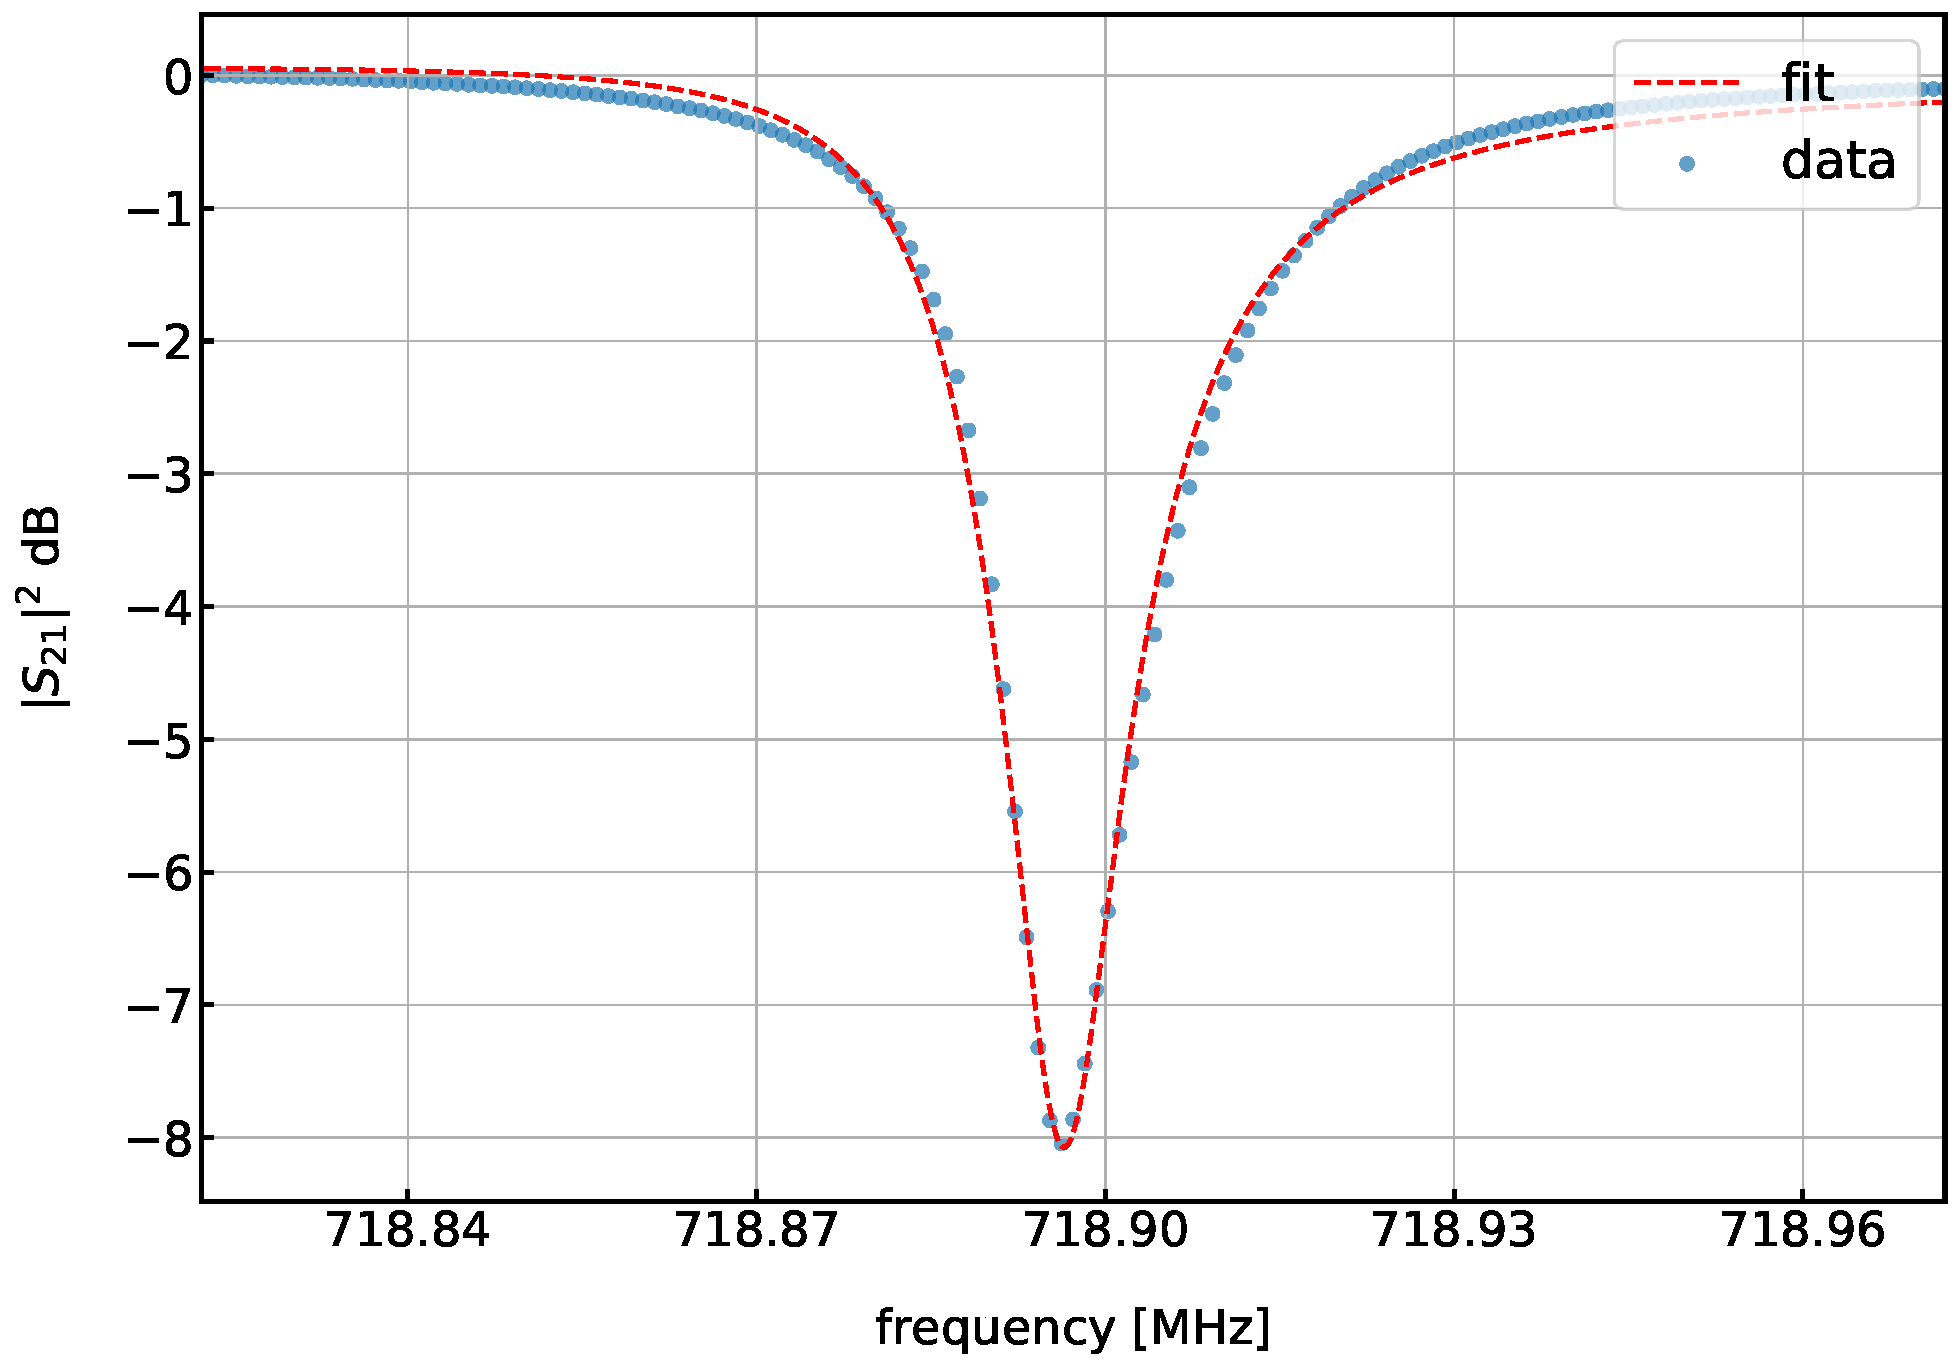
\includegraphics[scale=0.3]{figures/blast_data/timestreams/350_pal_S21_fit_448}
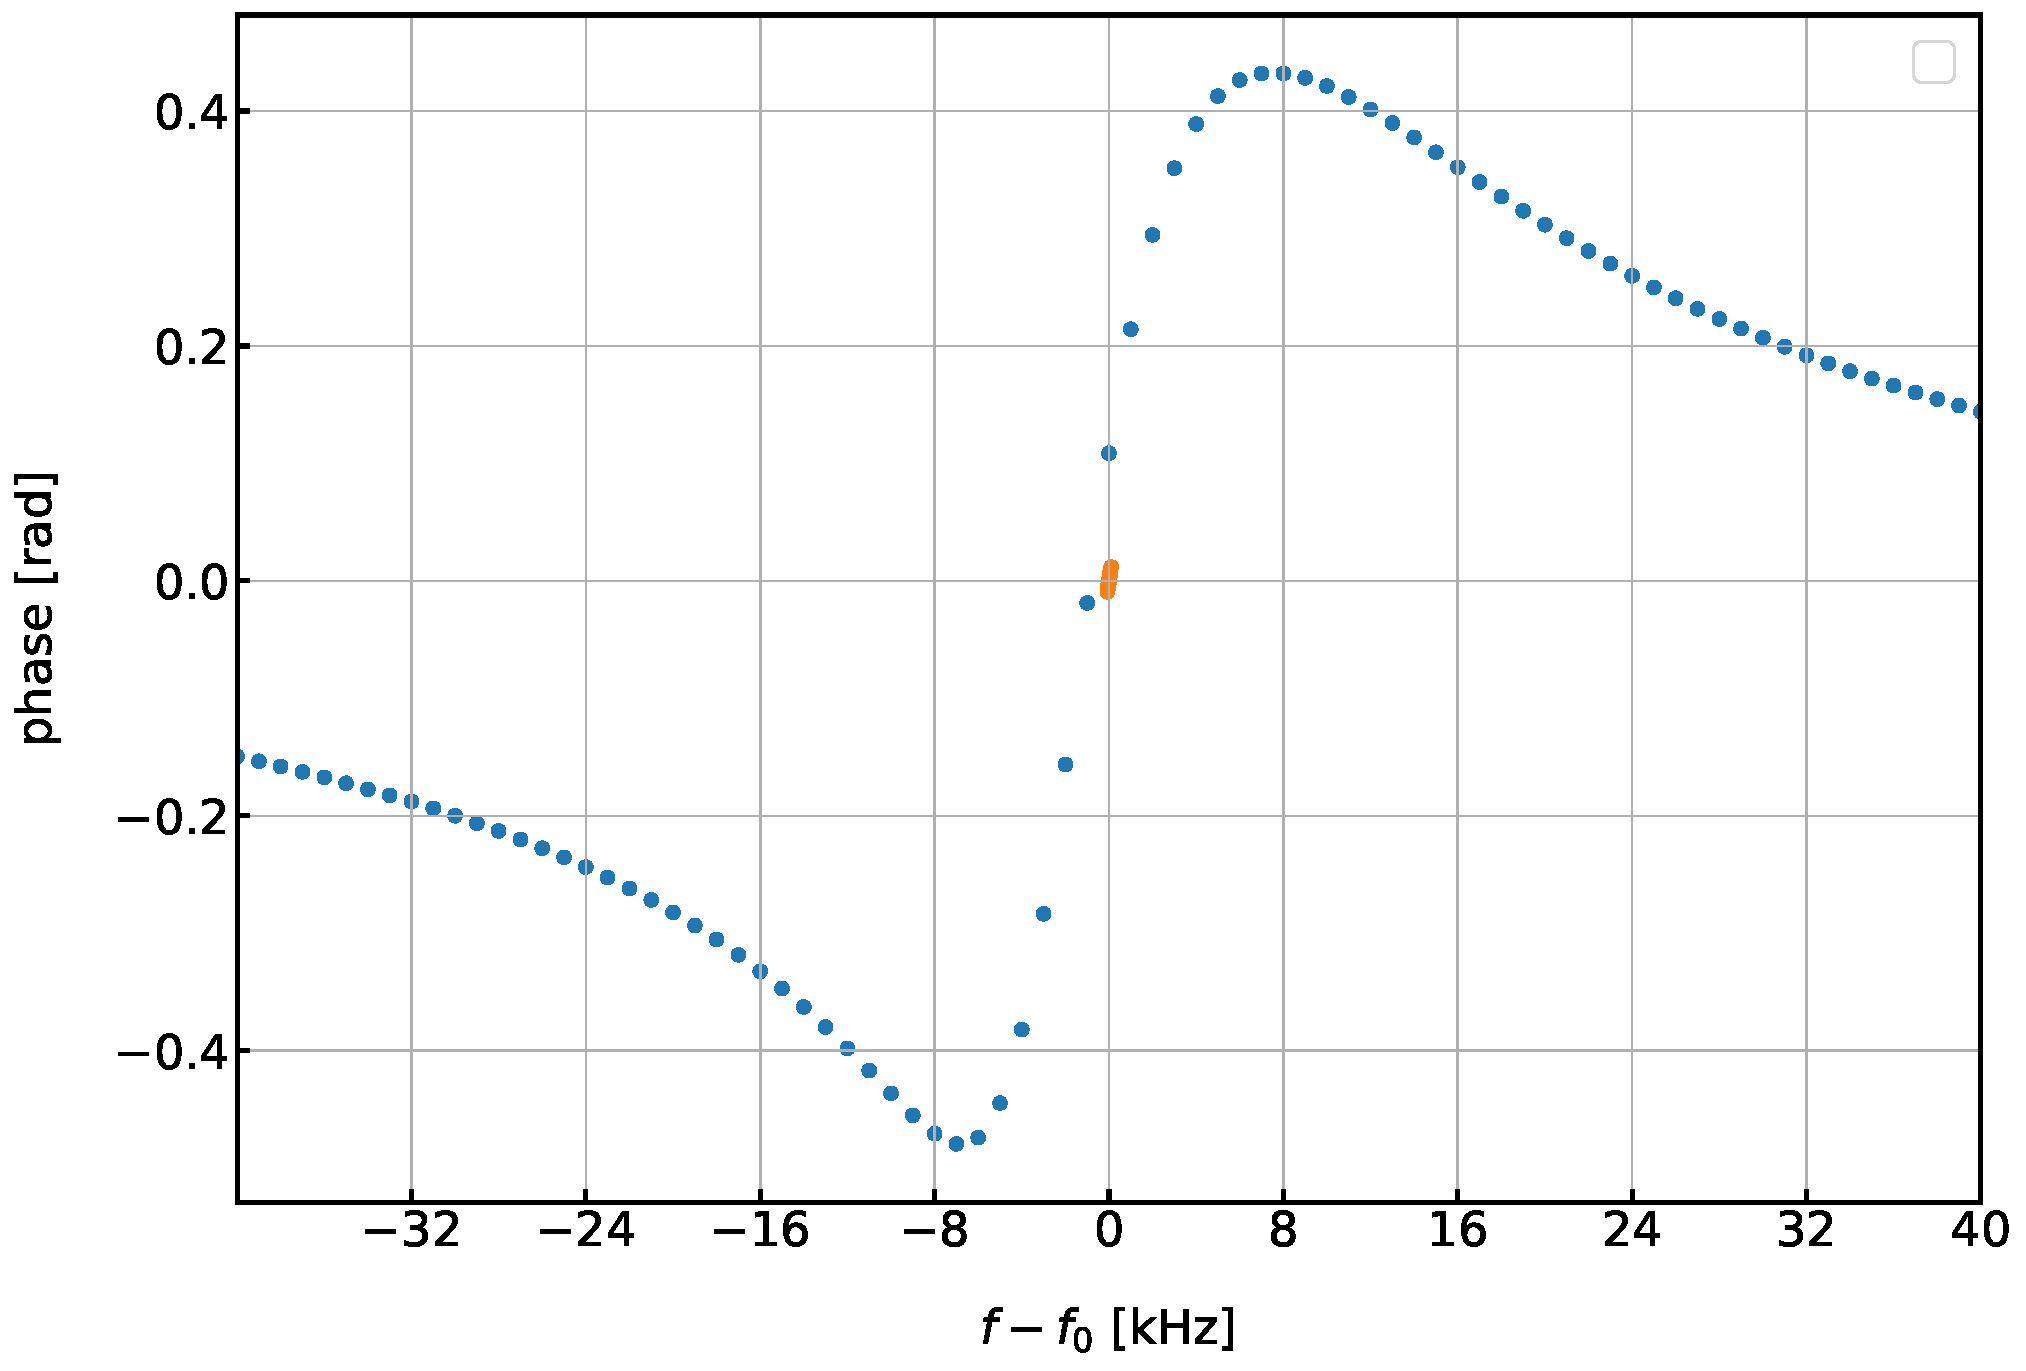
\includegraphics[scale=0.3]{figures/blast_data/timestreams/350_pal_freqNoiseBall_448}
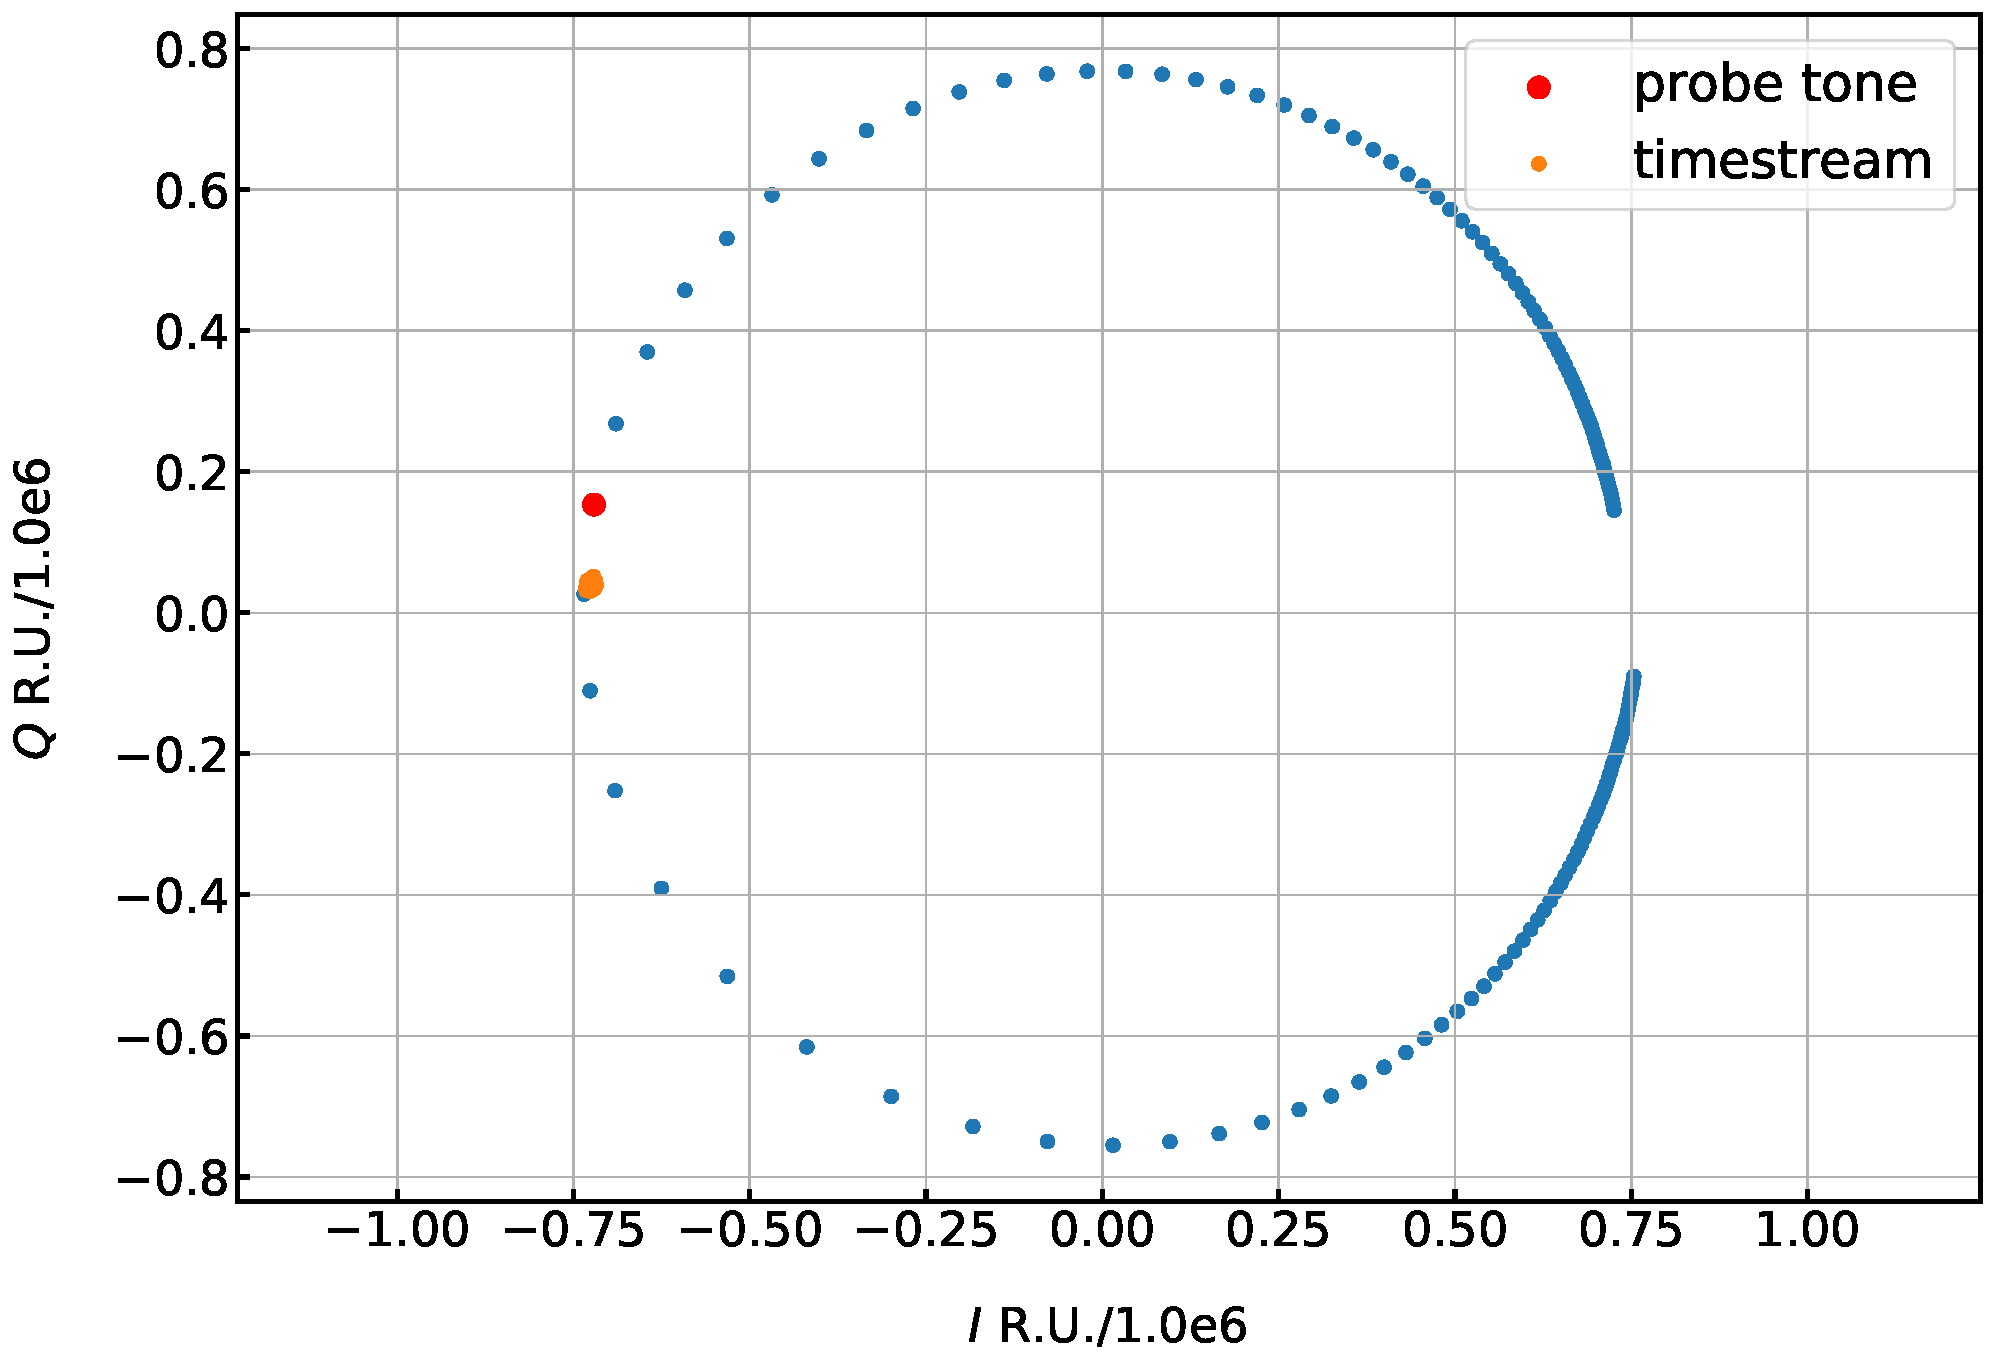
\includegraphics[scale=0.3]{figures/blast_data/timestreams/350_pal_noiseball_448}
\label{fig:example chan}
\end{figure}

\begin{table}[!htbp]
\centering
\begin{tabular}{@{}llllllll@{}}
\dtoprule{}
$f_{0}$ (MHz)   & Depth (dB) & \gls{Qr} & \gls{Qc} & \gls{Qi} & \gls{asym} & $(dI/df, dQ/df)$ (raw)  & \gls{Sff} (Hz$^{-1}$) \\ \midrule
718.90         & -8.04      & 32,826   & 54,460    & 83,3325   & 0.17  & -2.28, 127.68      & 2.78 $\times$ 10$^{-18}$    \\ \dbottomrule{}
\\
\end{tabular}
\caption[~Resonator parameters for channel 448 of the \macrocapwrap{350~$\upmu$m} array.]{Resonator parameters for channel 448 of the 350~$\upmu$m array.}
\label{table:350 example chan}
\end{table}

Using the resonator parameters which were fit from the \gls{S21} sweep and $I/Q$ timestream for channel 30, the frequency noise can be estimated without calculating the $I/Q$ gradient \gls{gradIQ} as:

\begin{equation}\label{eq:df estimate}
  \begin{aligned}
  e_{f} &= e_{v} \frac{f_{0} \gls{Qc} }{2 \gls{Qr}^{2}}\\
        &= \sqrt{ \frac{ (\sigma^{2}_{I} + \sigma^{2}_{Q}) / (f_{s}/2)}{ I^{2} + Q^{2} } } \frac{f_{0} \gls{Qc} }{2 \gls{Qr}^{2}} \qquad \left[  \frac{ \text{Hz} }{ \sqrt{\mathrm{Hz}} } \right]
  \end{aligned}
\end{equation}

where \gls{Qr} and \gls{Qc} are fit using the sweep, $f_{s}$ is the readout sampling frequency (e.g., 488.28125~Hz), and the voltage noise $e_{v}$ ($\mathrm{V}/\sqrt{\mathrm{Hz}})$ is calculated using $I/Q$ at their maximum off-resonance values for each channel.

Using the example channel values for $f_{0}$, \gls{Qr} and \gls{Qc} from Table~\ref{table:350 example chan} in Equation~\ref{eq:df estimate} gives $e_{f} \approx$ 1.5~$\mathrm{Hz}/\sqrt{\mathrm{Hz}}$. This is equal to the frequency noise calculated for this channel using the gradient method.

\begin{figure}[!htbp]
\centering
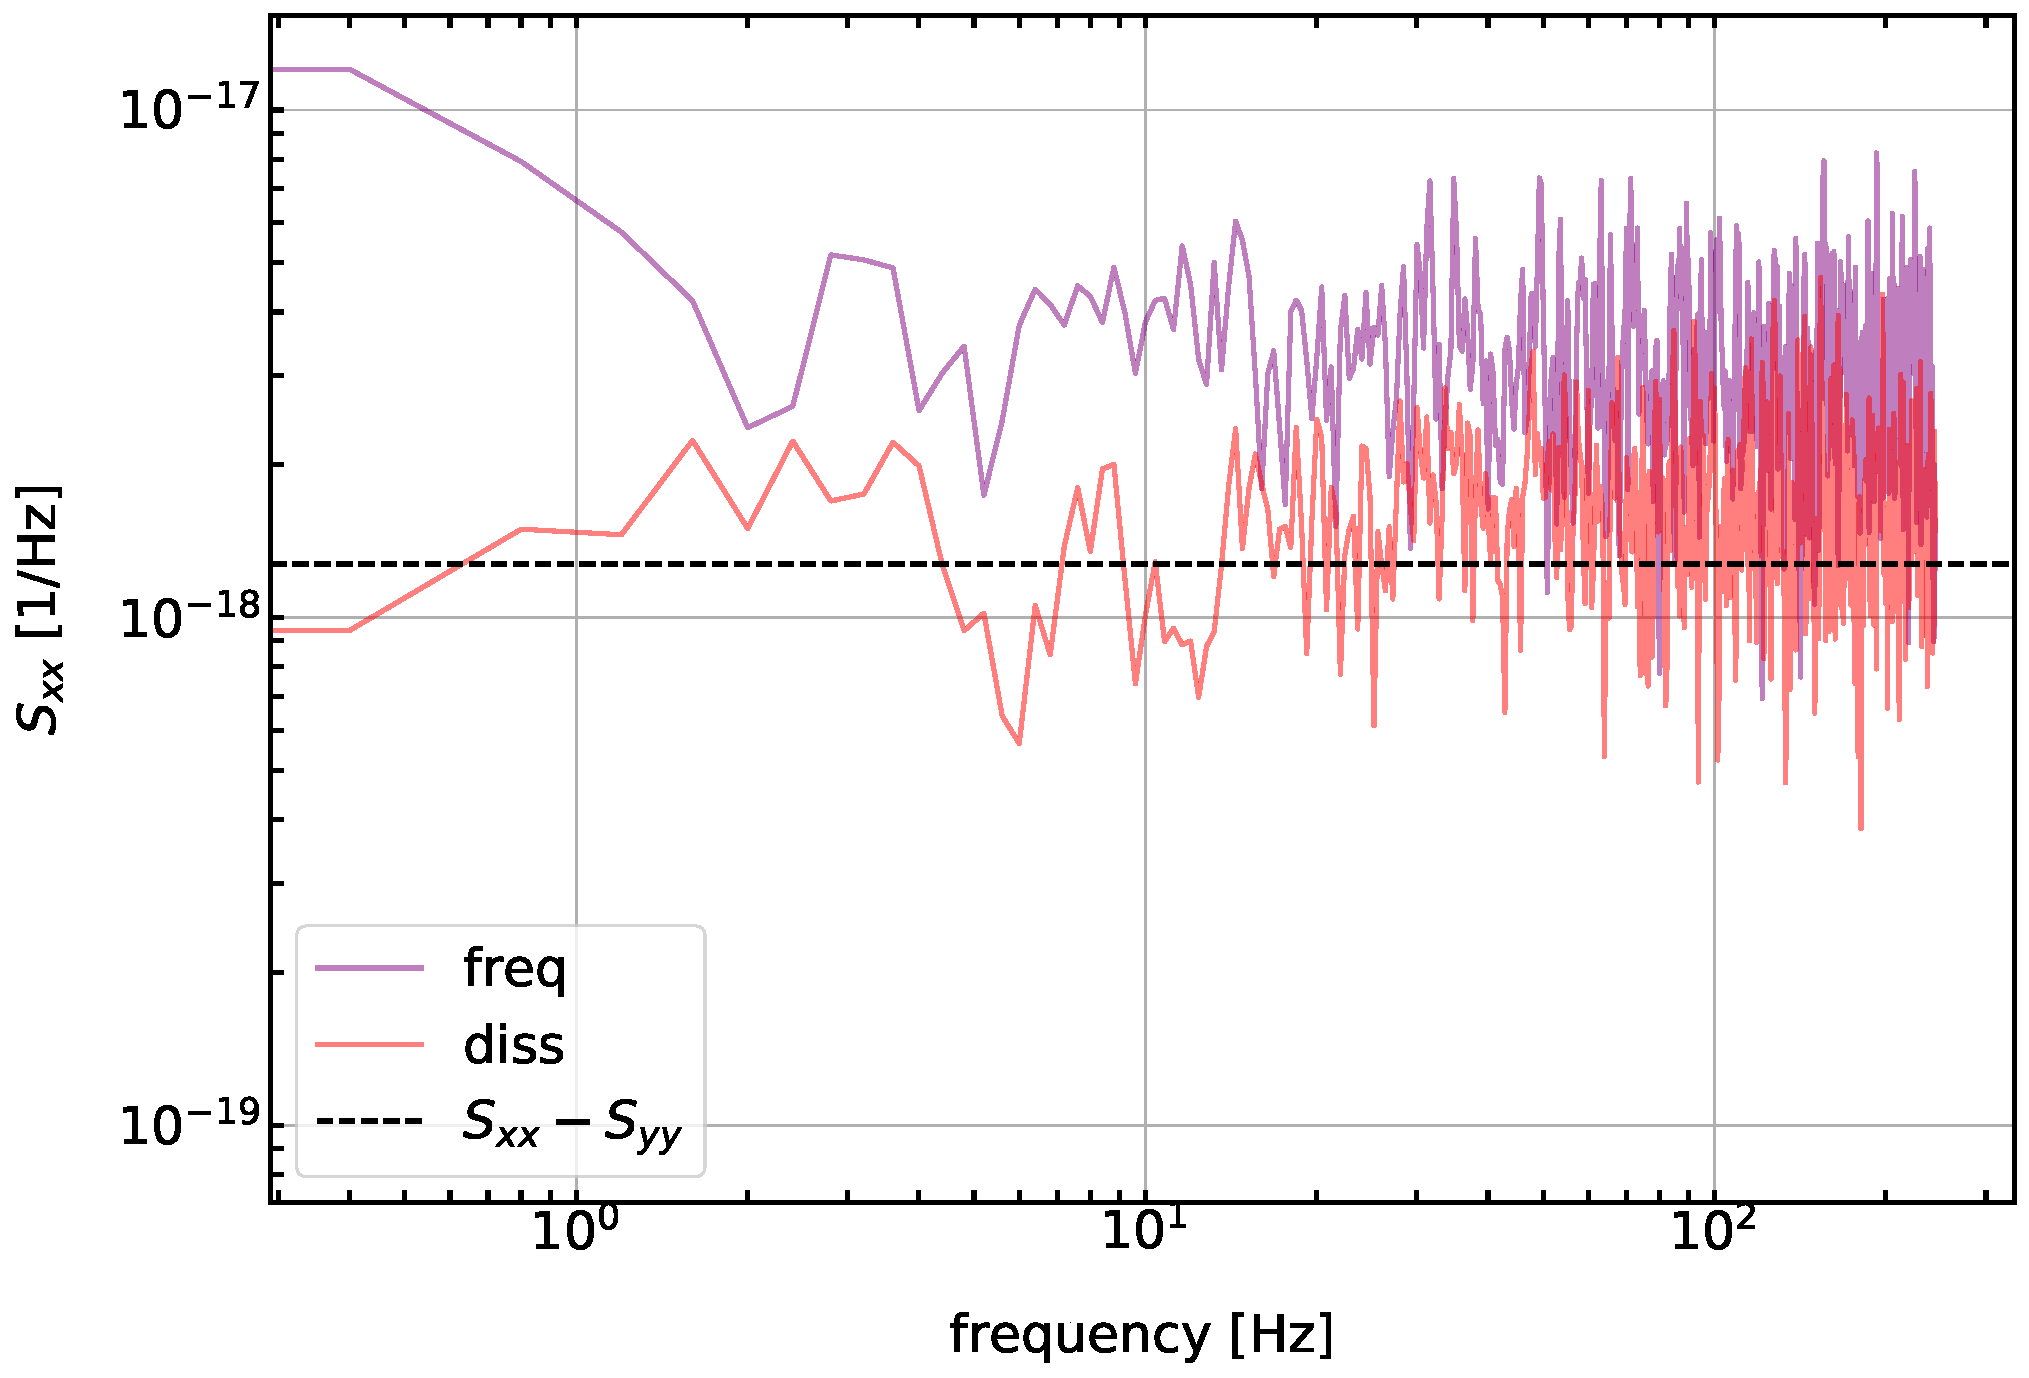
\includegraphics[width=\textwidth]{figures/blast_data/timestreams/350_448_freq_diss_psd}
\caption[~A 350~\macrocapwrap{$\upmu$m} channel PSD, showing the phase and dissipation quadratures.]{A 350~$\upmu$m channel PSD, showing \gls{Sxx} and \gls{Syy}.}
\label{fig:350 chan 448 psd}
\end{figure}

\begin{figure}[!htbp]
\centering
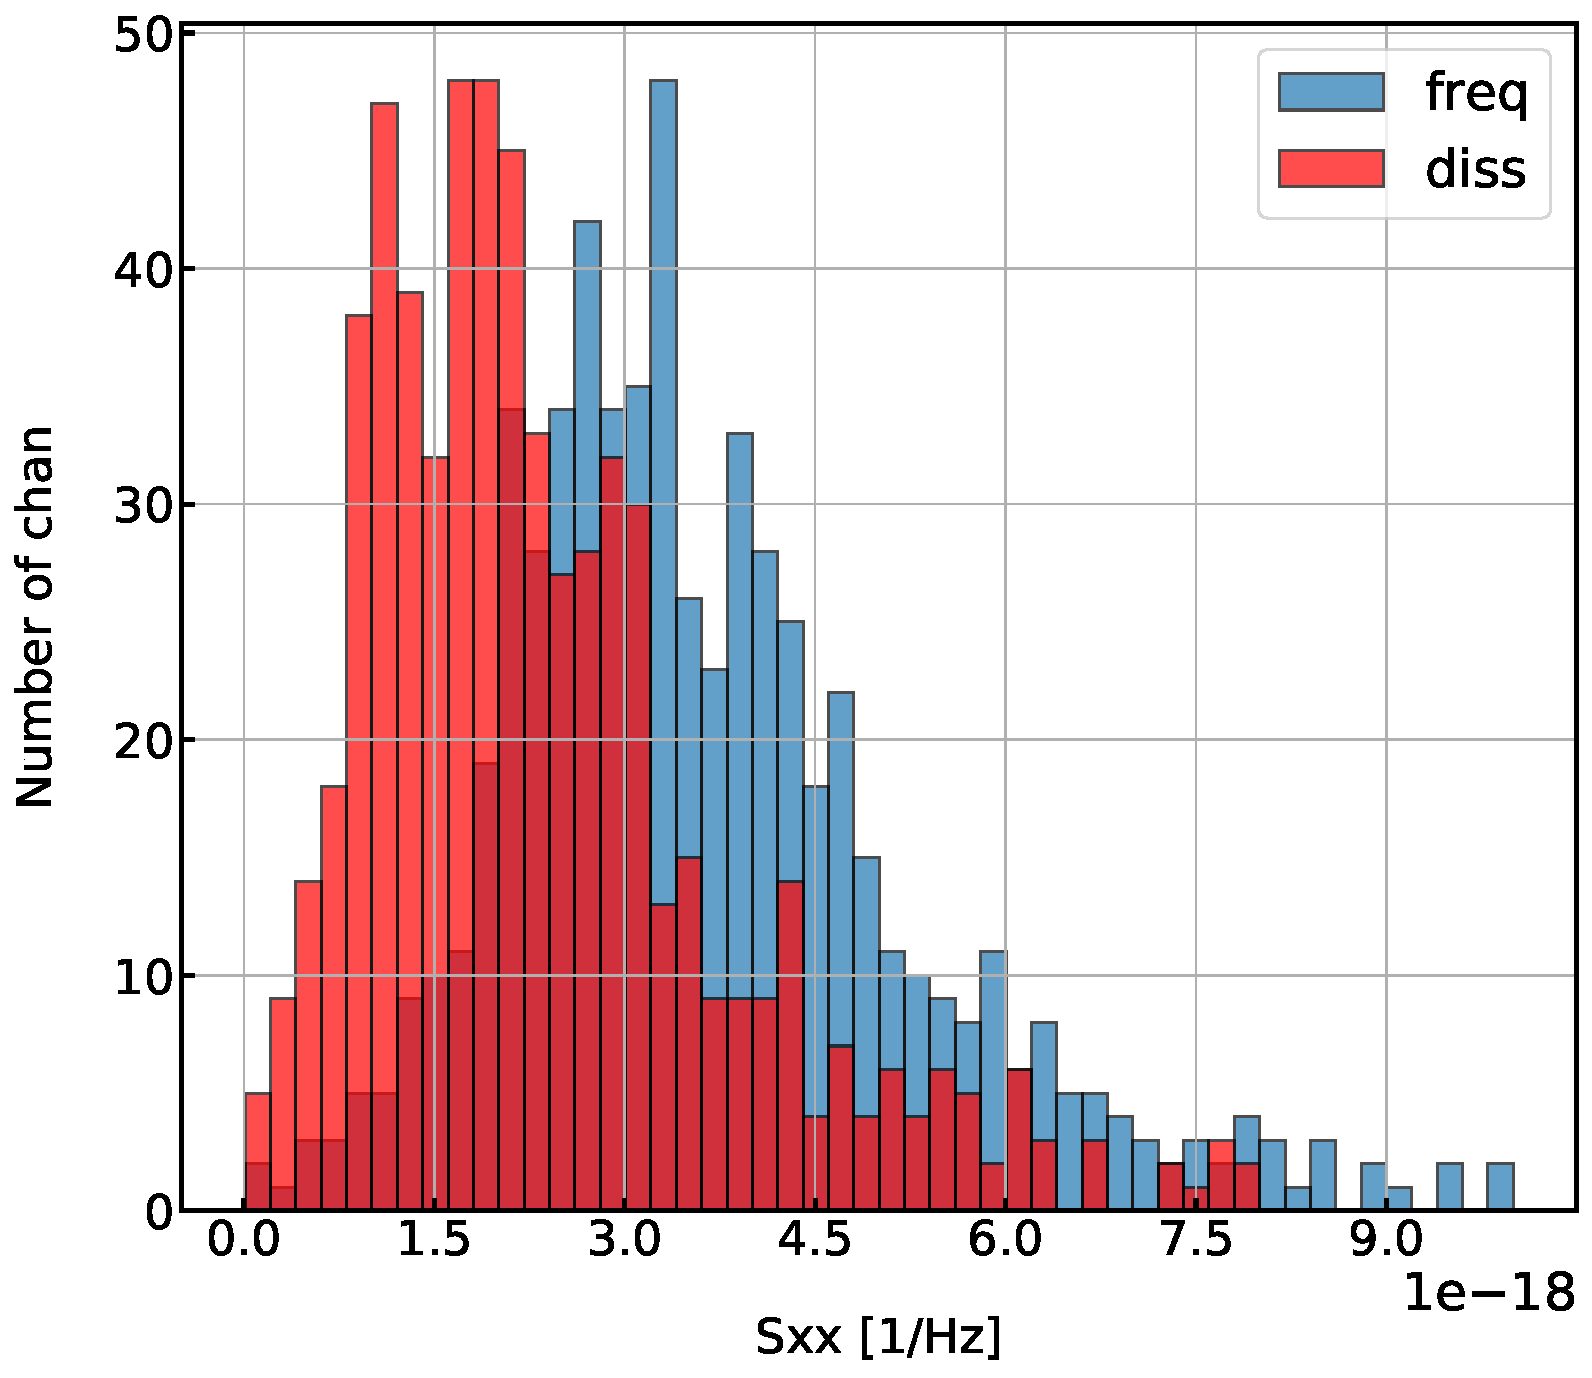
\includegraphics[width=\textwidth]{figures/blast_data/timestreams/350_pal_Sxx_hist_448}
\caption[~A histogram of frequency and dissipation noise for the 350~\macrocapwrap{$\upmu$m} array, as measured in Palestine, TX.]{A histogram of \gls{Sxx} and \gls{Syy} for the 350~$\upmu$m array, as measured in Palestine, TX.}
\label{fig:350 freq diss}
\end{figure}

\begin{comment}
\begin{figure}[!htbp]
\centering
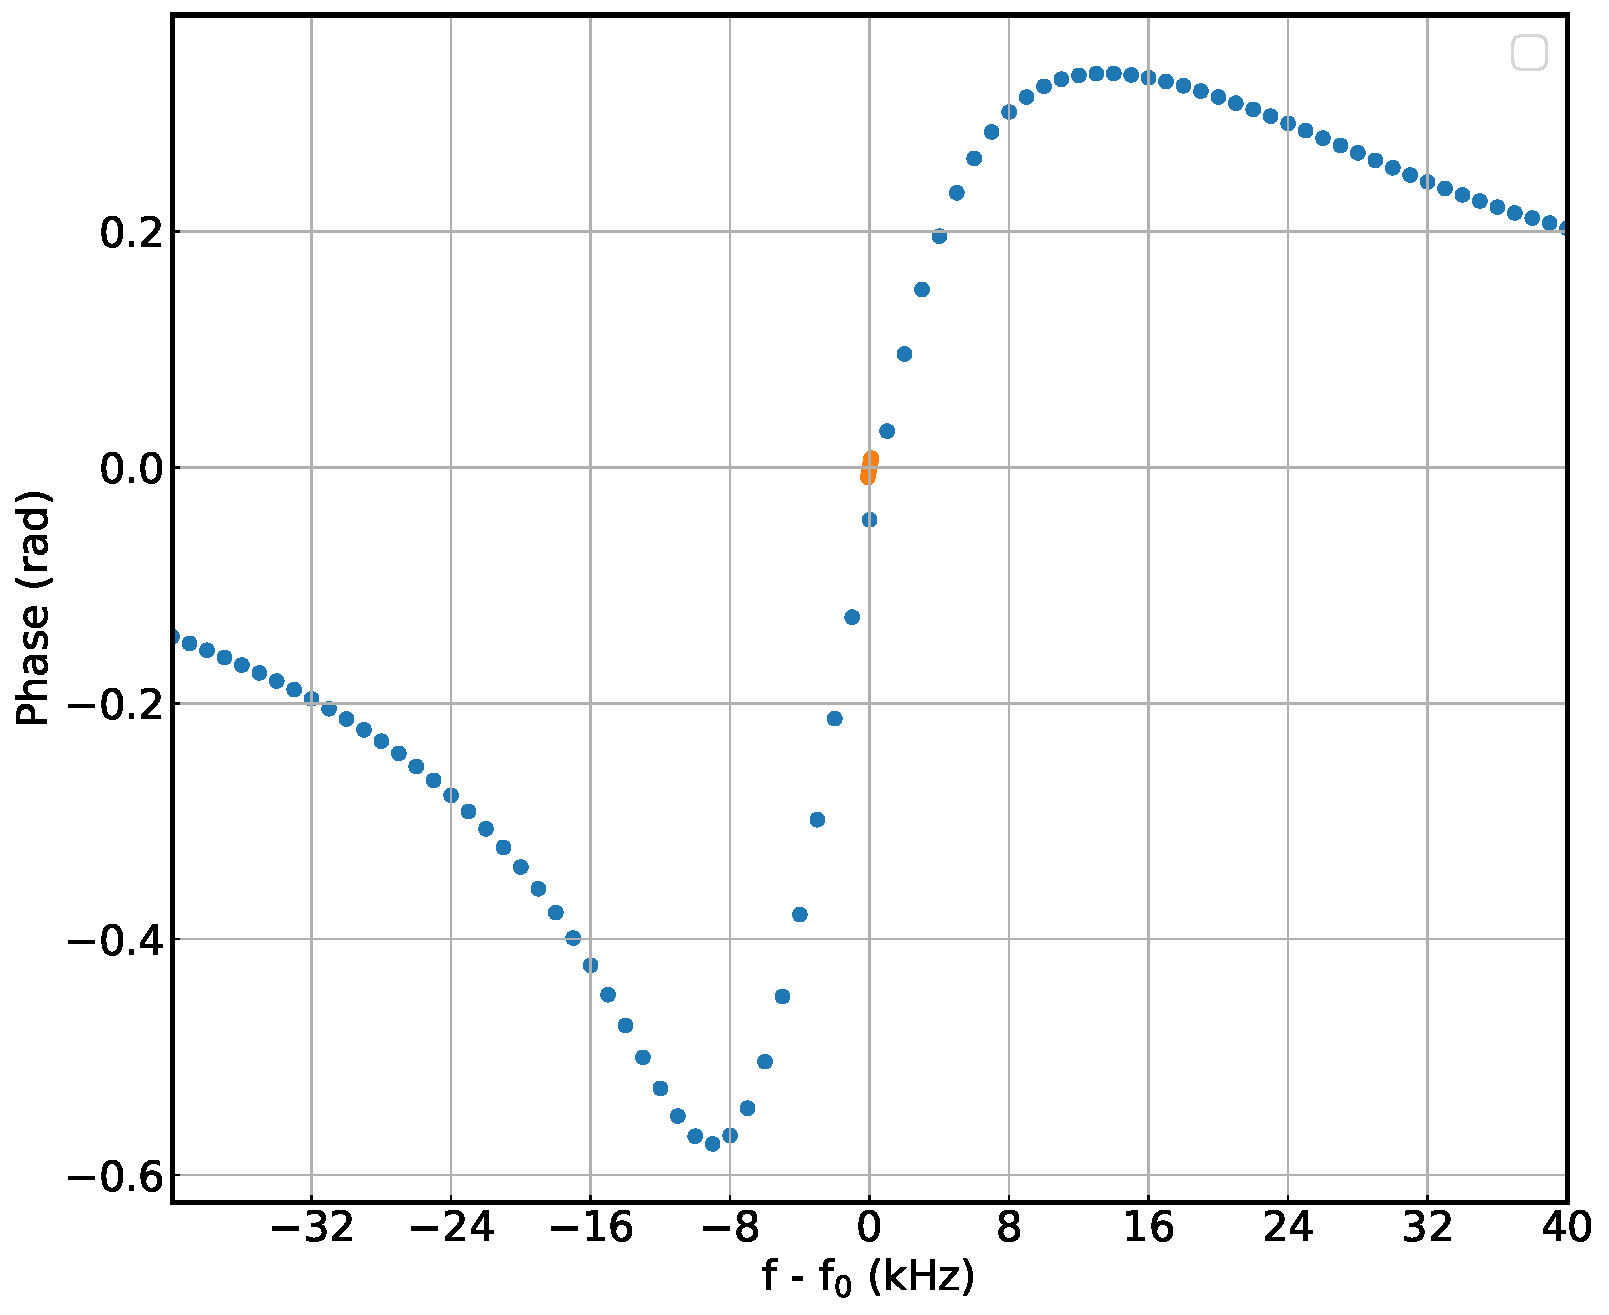
\includegraphics[width=\textwidth]{figures/blast_data/timestreams/350_pal_freqNoiseBall_30}
\caption[~A 250U ROACH2 sweep from Palestine, with a VNA sweep from May, 2018]{A 250U ROACH2 sweep (orange) from the Palestine integration, with a VNA sweep from May, 2018 (purple).}
\label{fig:freq noise ball}
\end{figure}

\begin{figure}[!htbp]
\centering
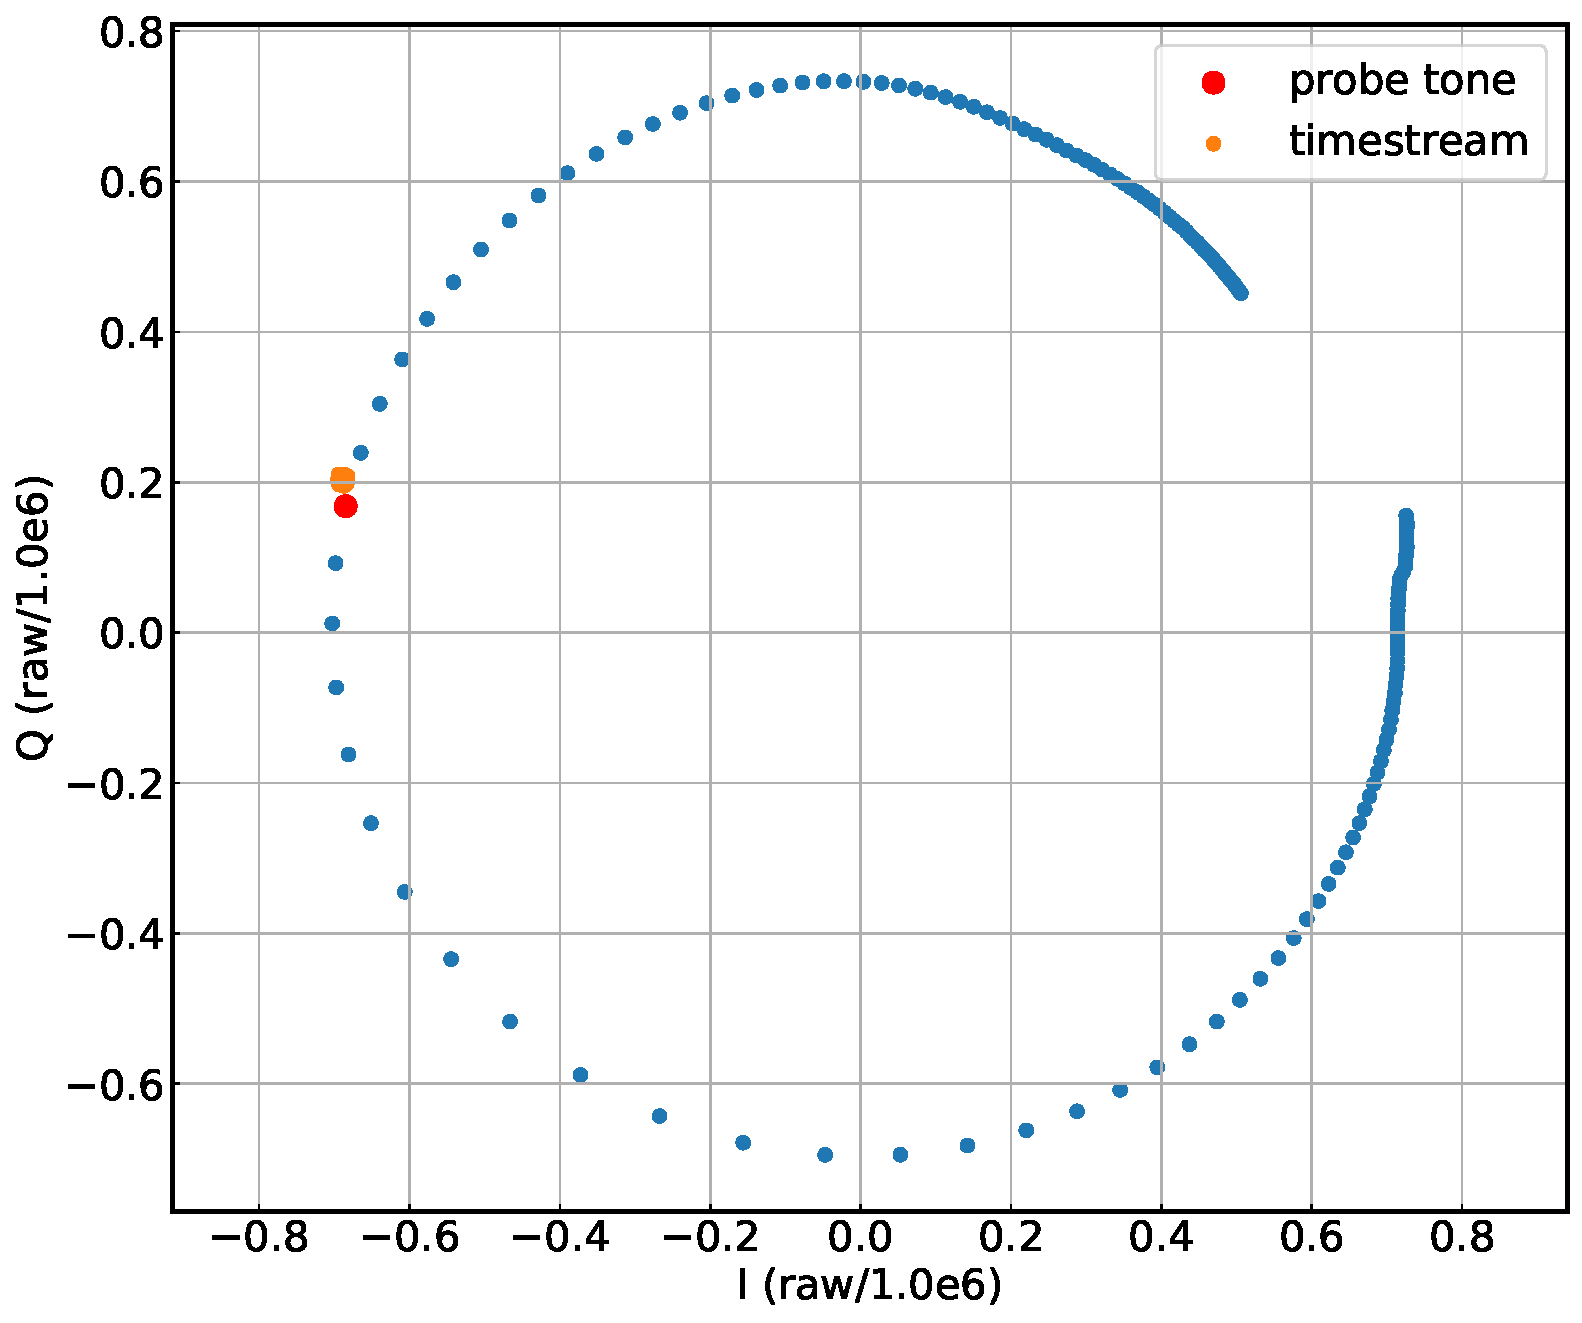
\includegraphics[width=\textwidth]{figures/blast_data/timestreams/350_pal_noiseball_30}
\caption[~Rotated and centered IQ circle for the Palestine 350~\macrocapwrap{$\upmu$m} example channel.]{Rotated and centered IQ circle for the Palestine 350~$\upmu$m example channel.}
\label{fig:IQ noise ball}
\end{figure}
\end{comment}

\subsection{Palestine Integration Detector Histograms}\label{histograms}

Because there are over 2,500 BLAST-TNG detectors, it would be impractical to present results for each one. Figures~\ref{fig:pal depth hist} to~\ref{fig:pal nep 250W} show histograms for the measured dip-depths, \gls{Qr}, \gls{Qr}/\gls{Qc}, and electrical NEP\@. The $I/Q$ timestreams used to produce these estimates was acquired during passband mapping, while the FTS was radiating into the cryostat window (see Section~\ref{fts}). No data containing interferograms was used in this analysis, although the level of optical loading on the detectors is assumed to be slightly higher than the ambient 290~K of the CSBF highbay. Throughout the measurement, A 4\% cryogenic NDF was present in the optical chain. The median values for each of the measured quantities is listed in Table~\ref{table:palestine hists}. The values for the electrical NEP will be used to convert to noise-equivalent flux density in Section~\ref{nefd}.

\begin{table}[!htbp]
\centering
\caption[~Median values of important detector parameters for all five BLAST-TNG arrays, measured at CSBF.]{Median values of important detector parameters for all five BLAST-TNG arrays, measured at CSBF.}
\label{table:palestine hists}
\begin{tabular}{@{}llllll@{}}
\dtoprule{}
 & 500~$\upmu$m & 250V & 350~$\upmu$m & 250U & 250W \\ \midrule
\gls{Qr} & 5361 & 12,759 & 12,759 & 17,301 & 16,942 \\
\gls{Qr}/\gls{Qc} & 0.073 & 0.28 & 0.56 & 0.24 & 0.22 \\
Depth (dB) & -0.74 & -3.22 & -7.81 & -2.52 & -2.28 \\
\gls{Sxx} (1/Hz) & 28 $\times$ 10$^{-17}$ & 30 $\times$ 10$^{-17}$ & 0.34 $\times$ 10$^{-17}$ & 3.5 $\times$ 10$^{-17}$ & 4 $\times$ 10$^{-17}$ \\
\gls{Syy} (1/Hz) & 25 $\times$ 10$^{-17}$ & 27 $\times$ 10$^{-17}$ & 0.21 $\times$ 10$^{-17}$ & 2.4 $\times$ 10$^{-17}$ & 2.5 $\times$ 10$^{-17}$ \\
NEP$_{\mathrm{freq}}$ W/$\sqrt{\mathrm{Hz}}$ & 10 $\times$ 10$^{-17}$ & 100 $\times$ 10$^{-17}$ & 35 $\times$ 10$^{-17}$ & 35 $\times$ 10$^{-17}$ & 37 $\times$ 10$^{-17}$ \\ \dbottomrule{}
\\
\end{tabular}
\end{table}

\begin{figure}[!htbp]
\centering
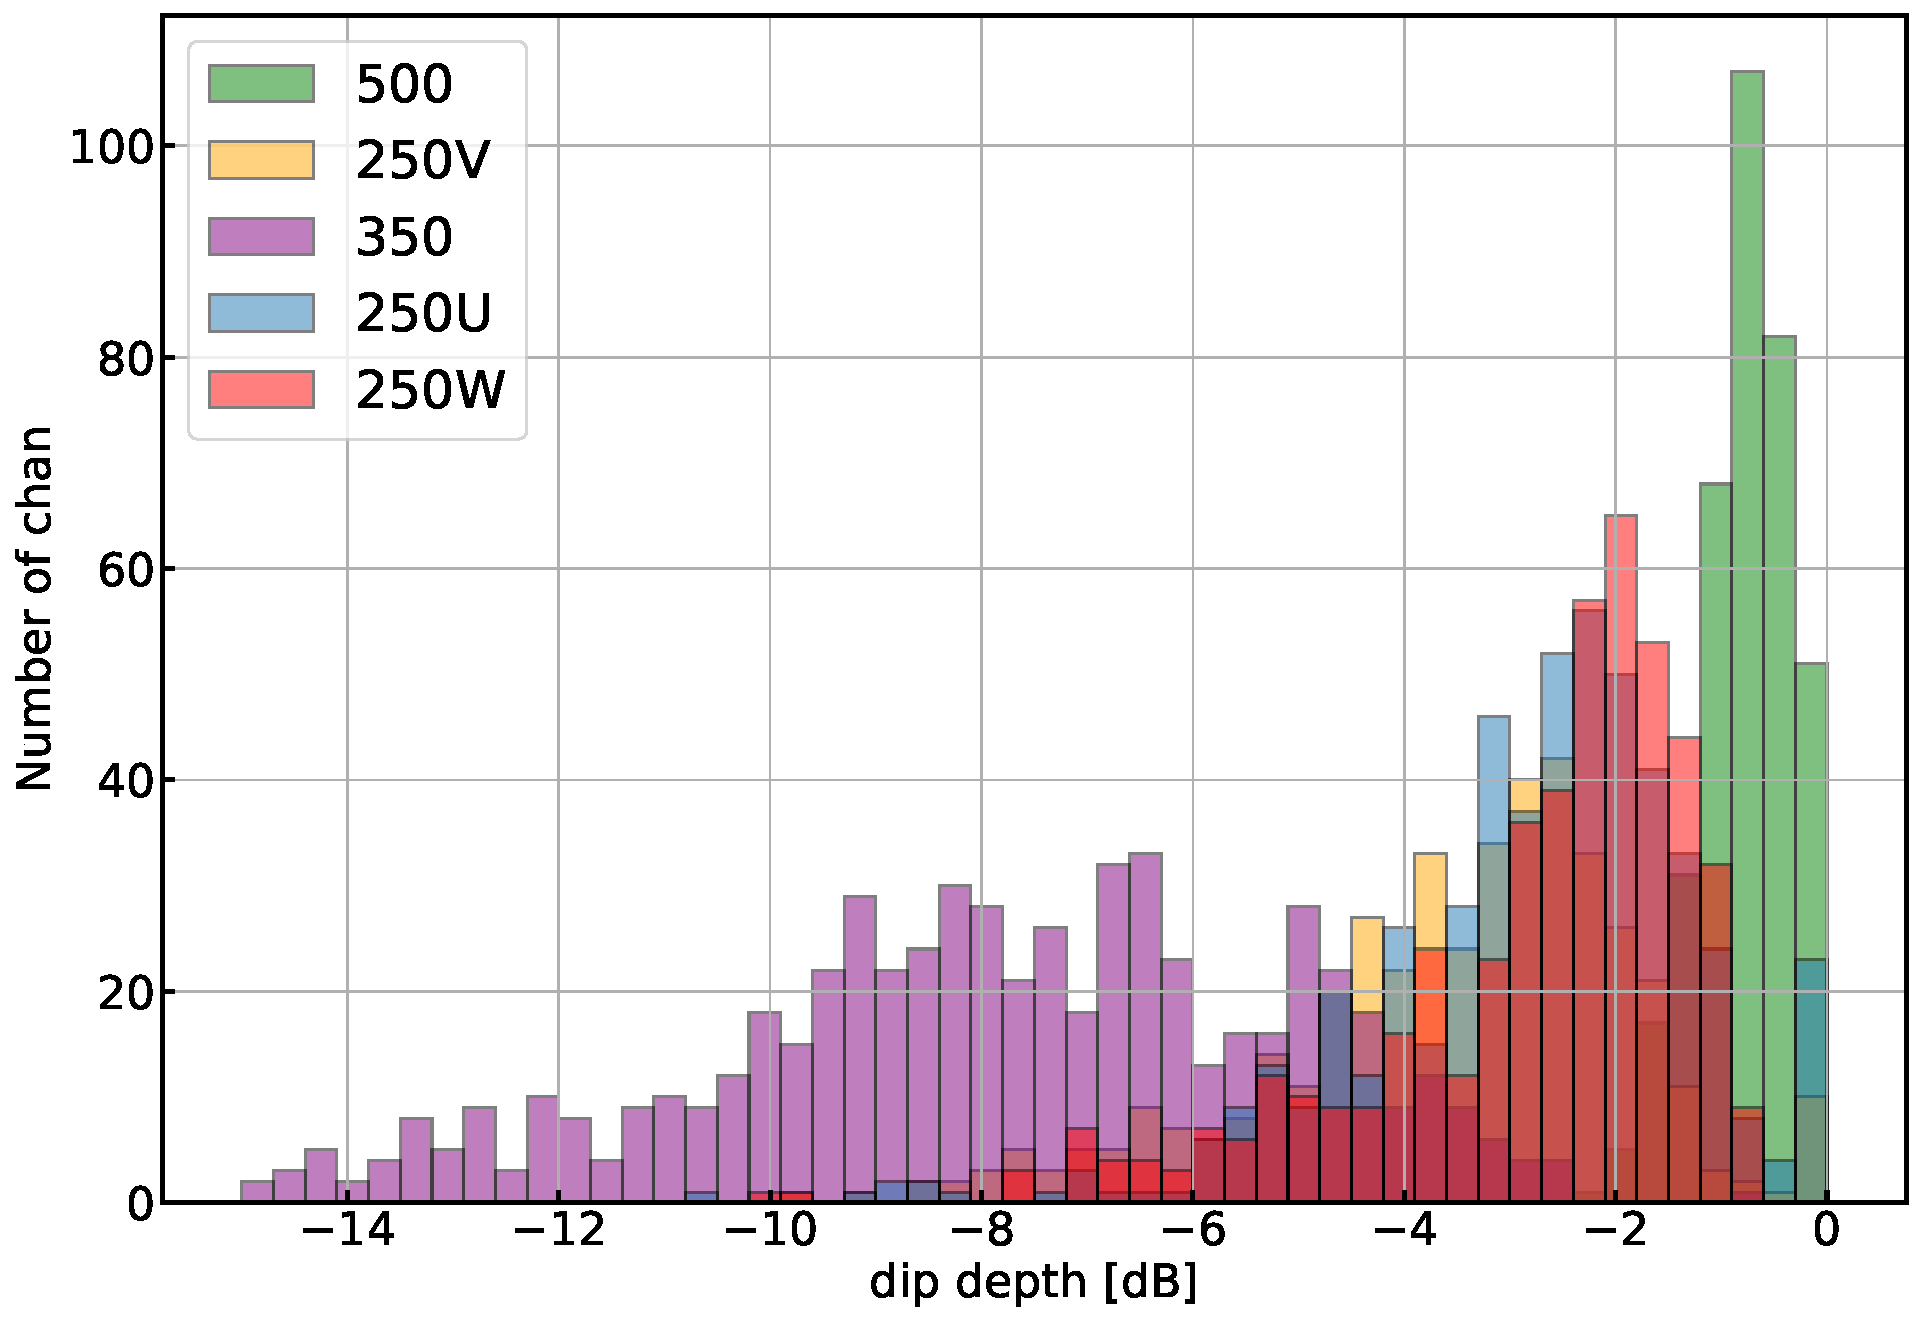
\includegraphics[width=\textwidth]{figures/blast_data/hist/PAL_depth_hist}
\caption[~Histograms of resonator dip-depth for all five BLAST-TNG arrays, measured at CSBF.]{Histograms of resonator dip-depth for all five BLAST-TNG arrays, measured at CSBF.}
\label{fig:pal depth hist}
\end{figure}

\begin{figure}[!htbp]
\centering
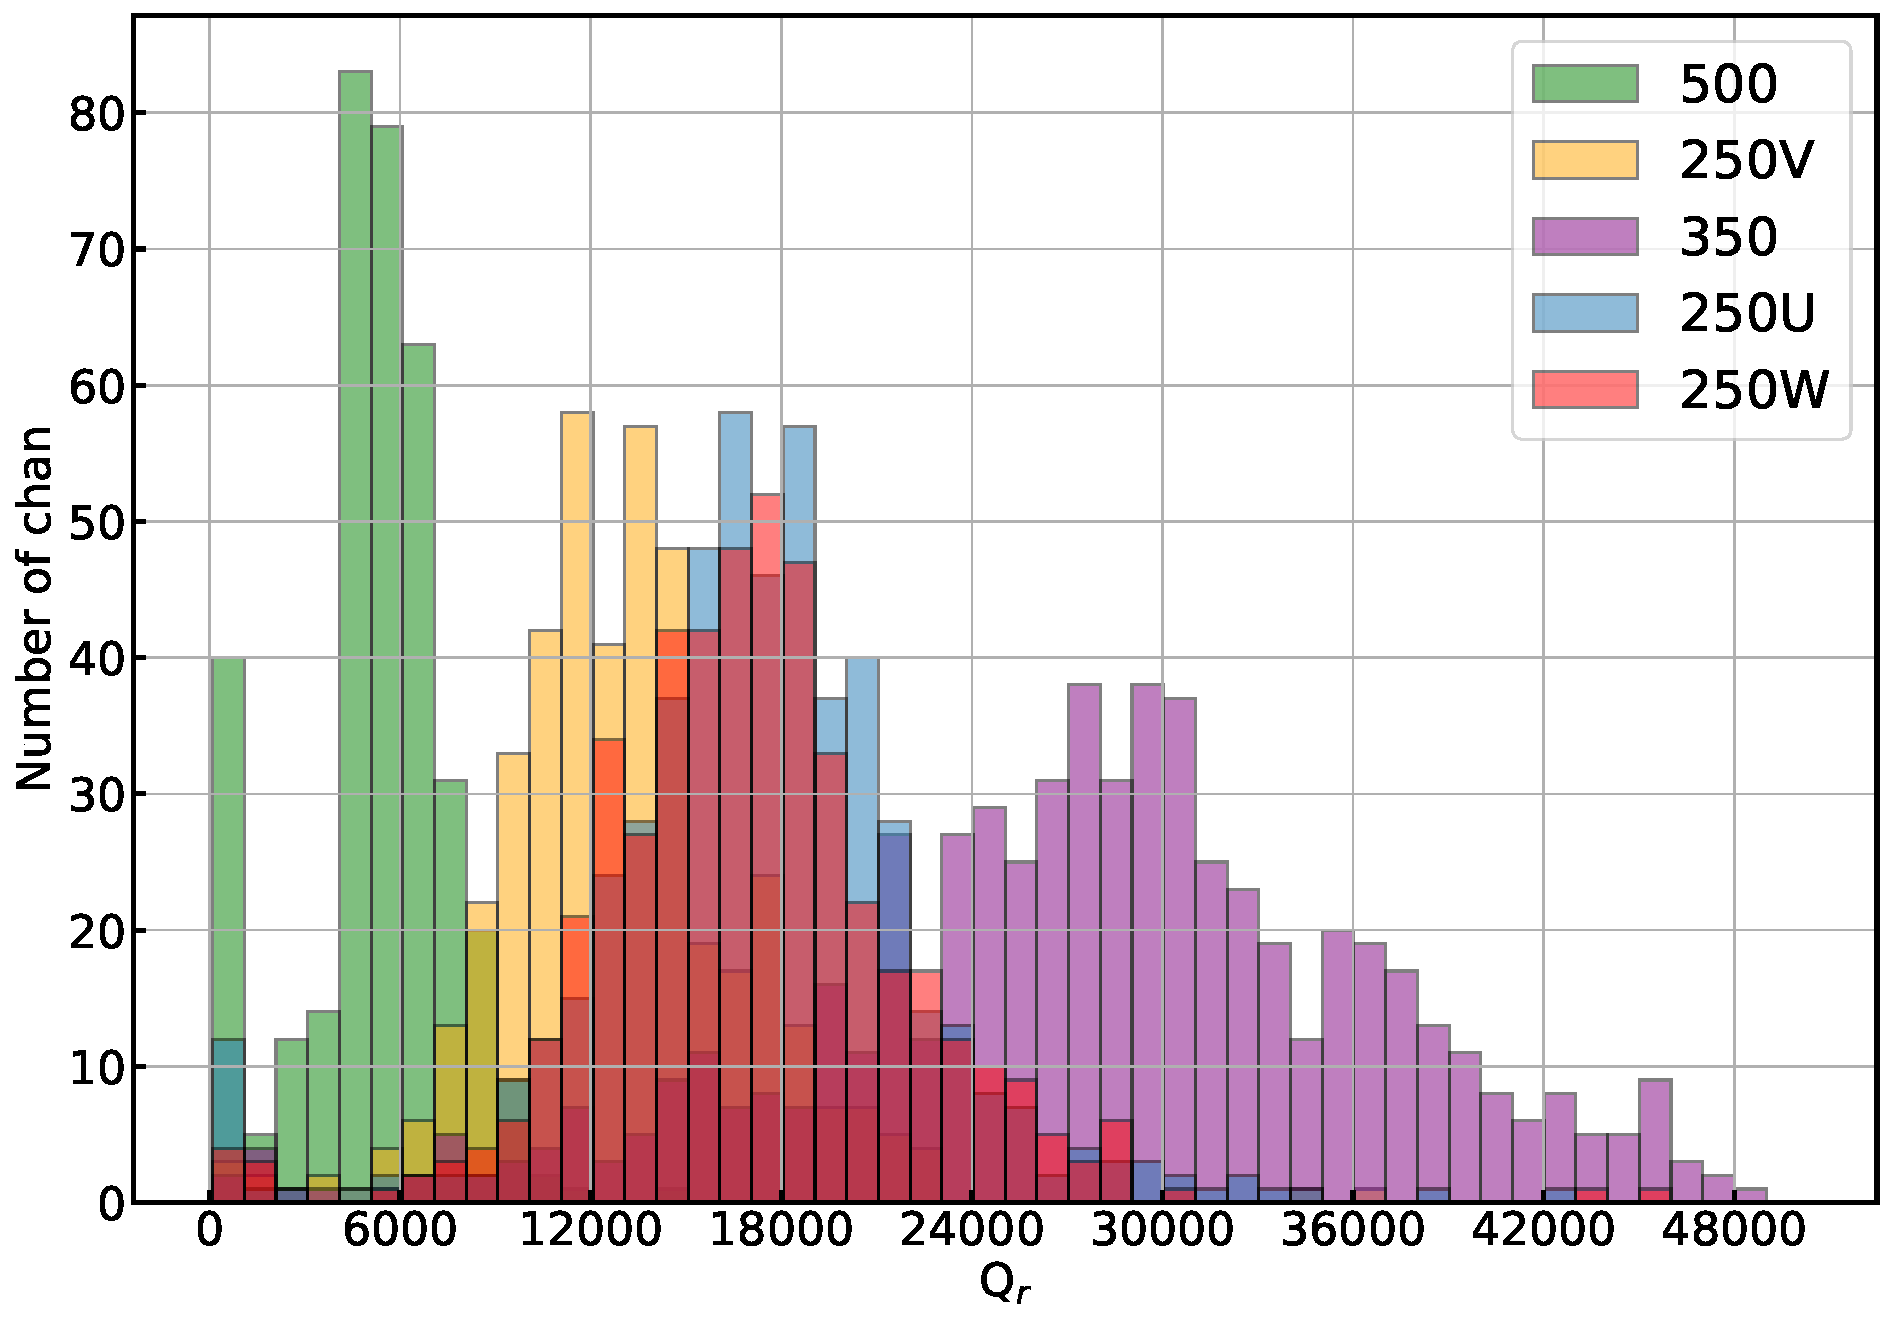
\includegraphics[width=\textwidth]{figures/blast_data/hist/PAL_Qr_hist}
\caption[~Histograms of \macrocapwrap{\gls{Qr}} for all five BLAST-TNG arrays, measured at CSBF.]{Histograms of \gls{Qr} for all five BLAST-TNG arrays, measured at CSBF.}
\label{fig:pal qr hist}
\end{figure}

\begin{figure}[!htbp]
\centering
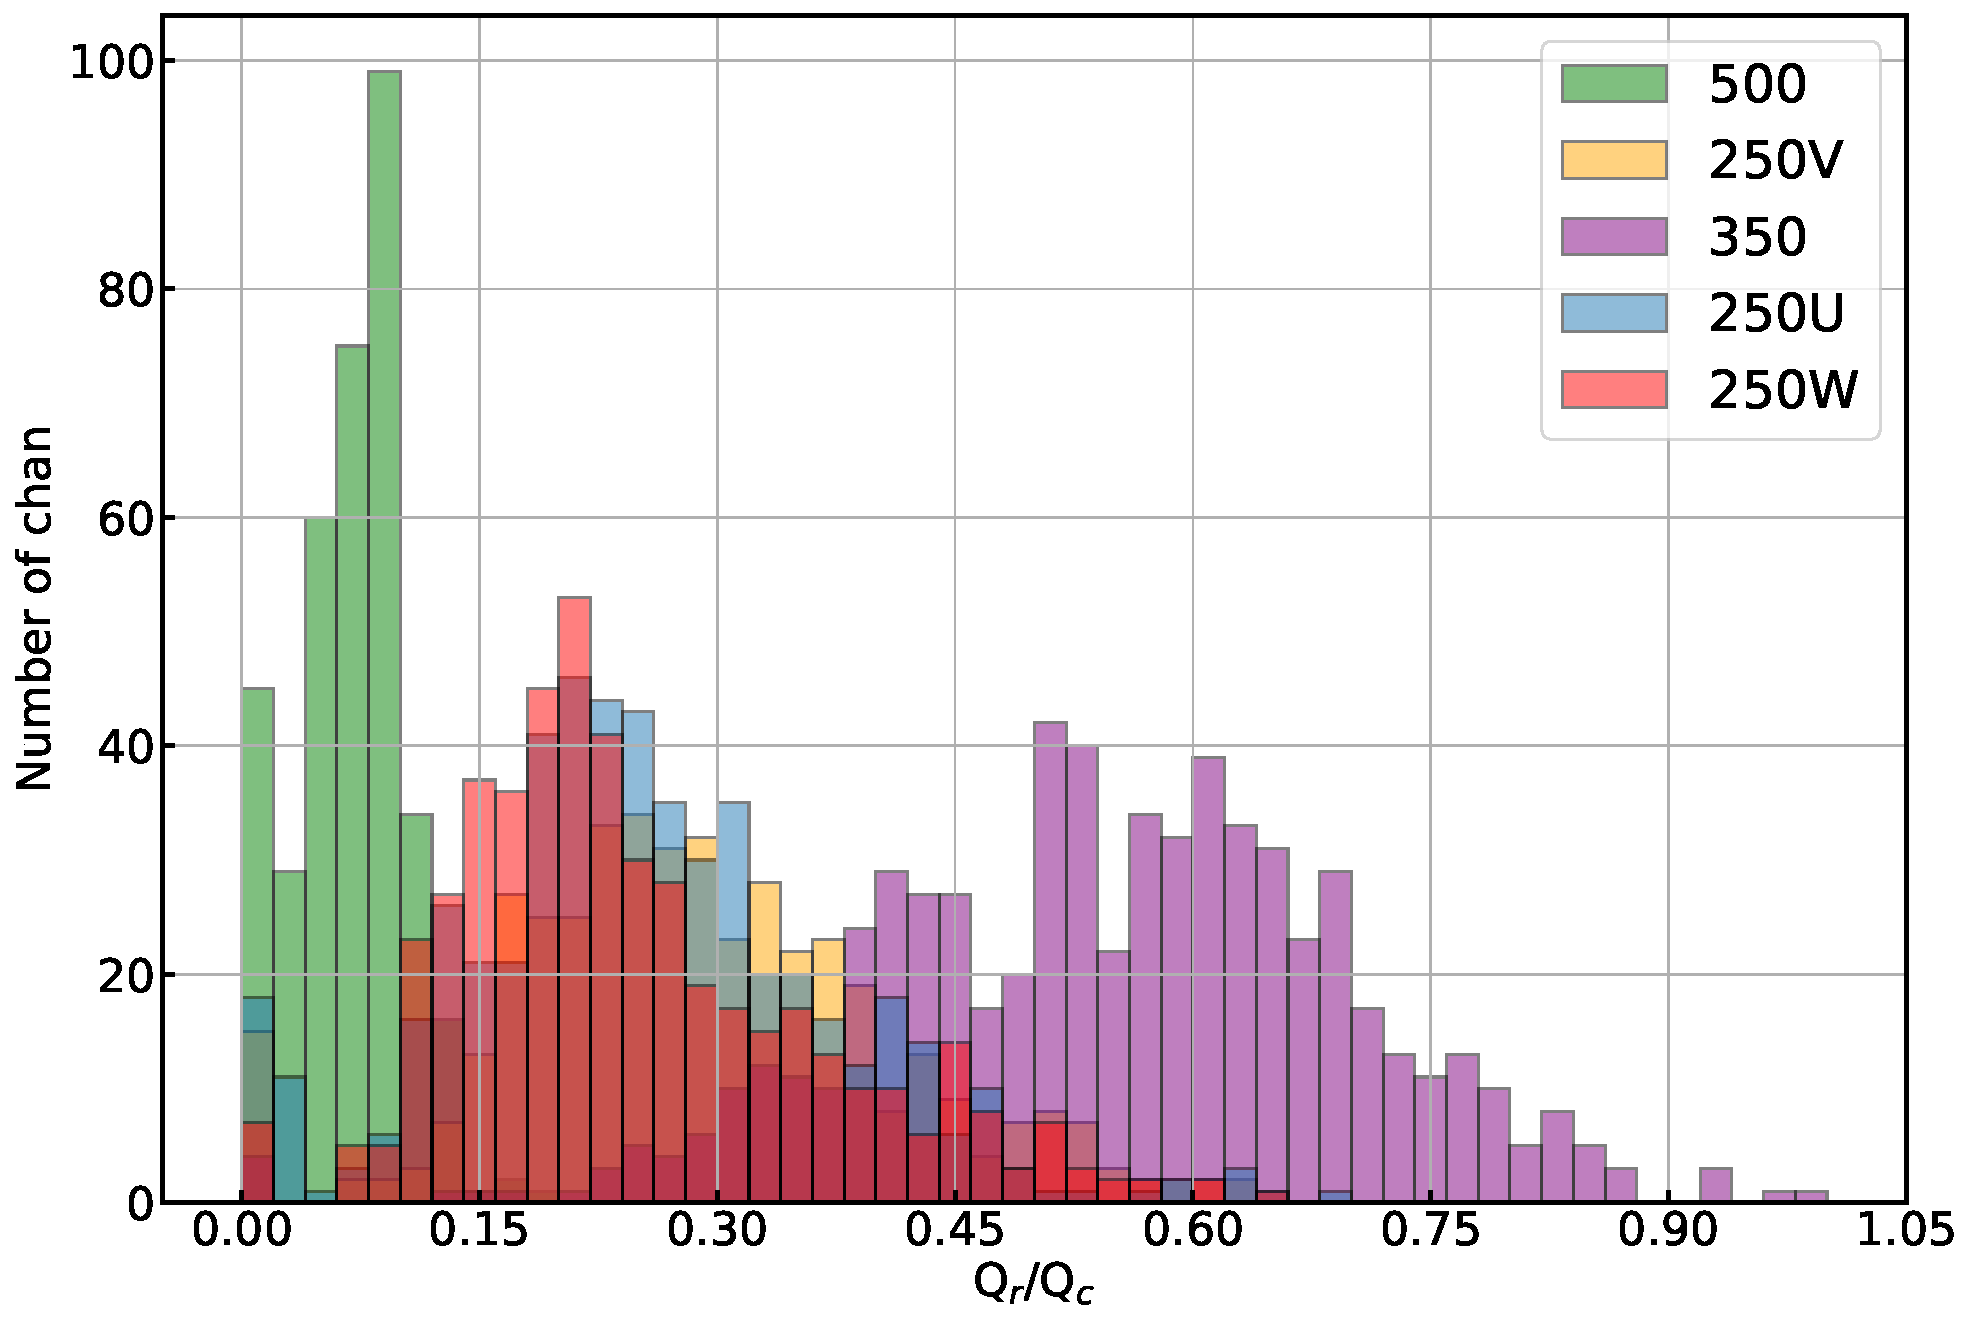
\includegraphics[width=\textwidth]{figures/blast_data/hist/PAL_QrQc_hist}
\caption[~Histograms of \macrocapwrap{\gls{Qr}/\gls{Qc}} for all five BLAST-TNG arrays, measured at CSBF.]{Histograms of \gls{Qr}/\gls{Qc} for all five BLAST-TNG arrays, measured at CSBF.}
\label{fig:pal qrqc hist}
\end{figure}

\begin{figure}[!htbp]
\centering
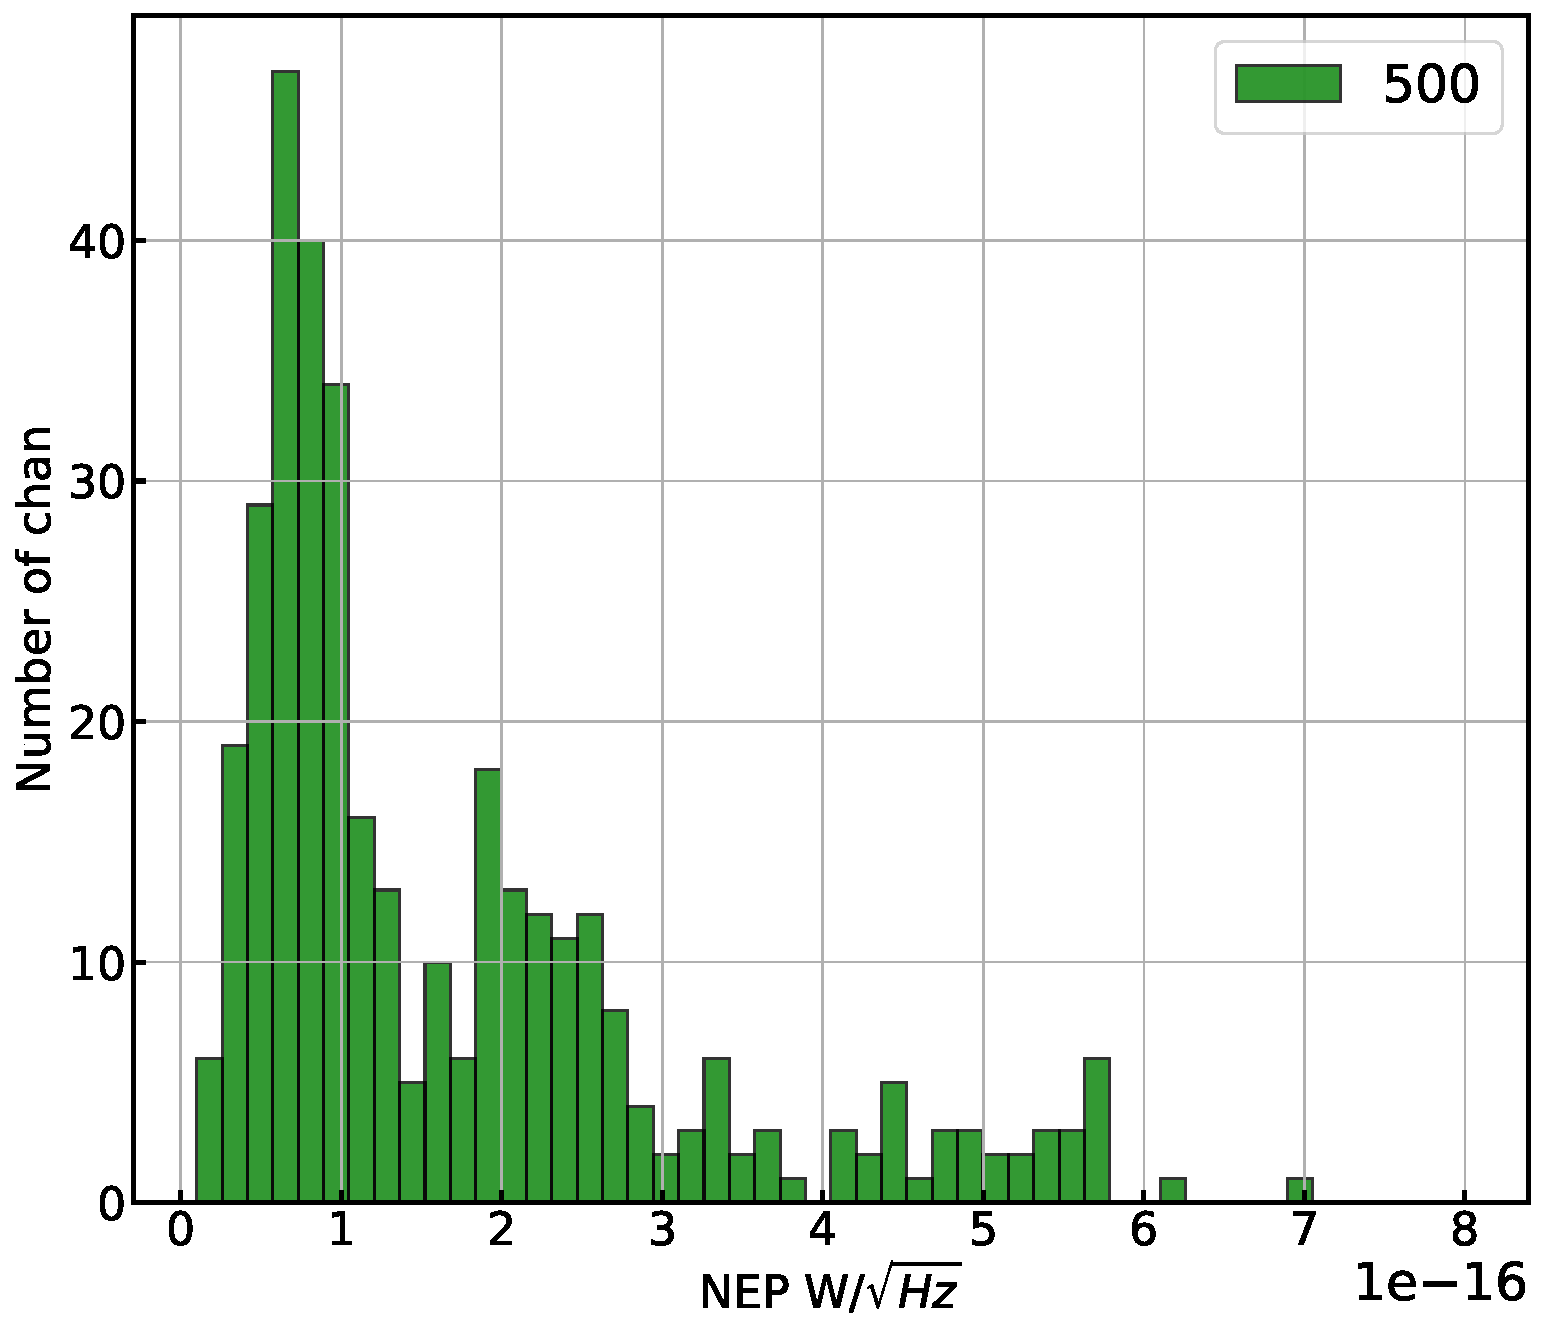
\includegraphics[width=\textwidth]{figures/blast_data/hist/PAL_NEP_hist_R1}
\caption[~Histogram of \macrocapwrap{NEP$_{\mathrm{freq}}$} for the 500~\macrocapwrap{$\upmu$m} array, measured at CSBF.]{Histogram of NEP$_{\mathrm{freq}}$ for the 500~$\upmu$m array, measured at CSBF.}
\label{fig:pal nep 500}
\end{figure}

\begin{figure}[!htbp]
\centering
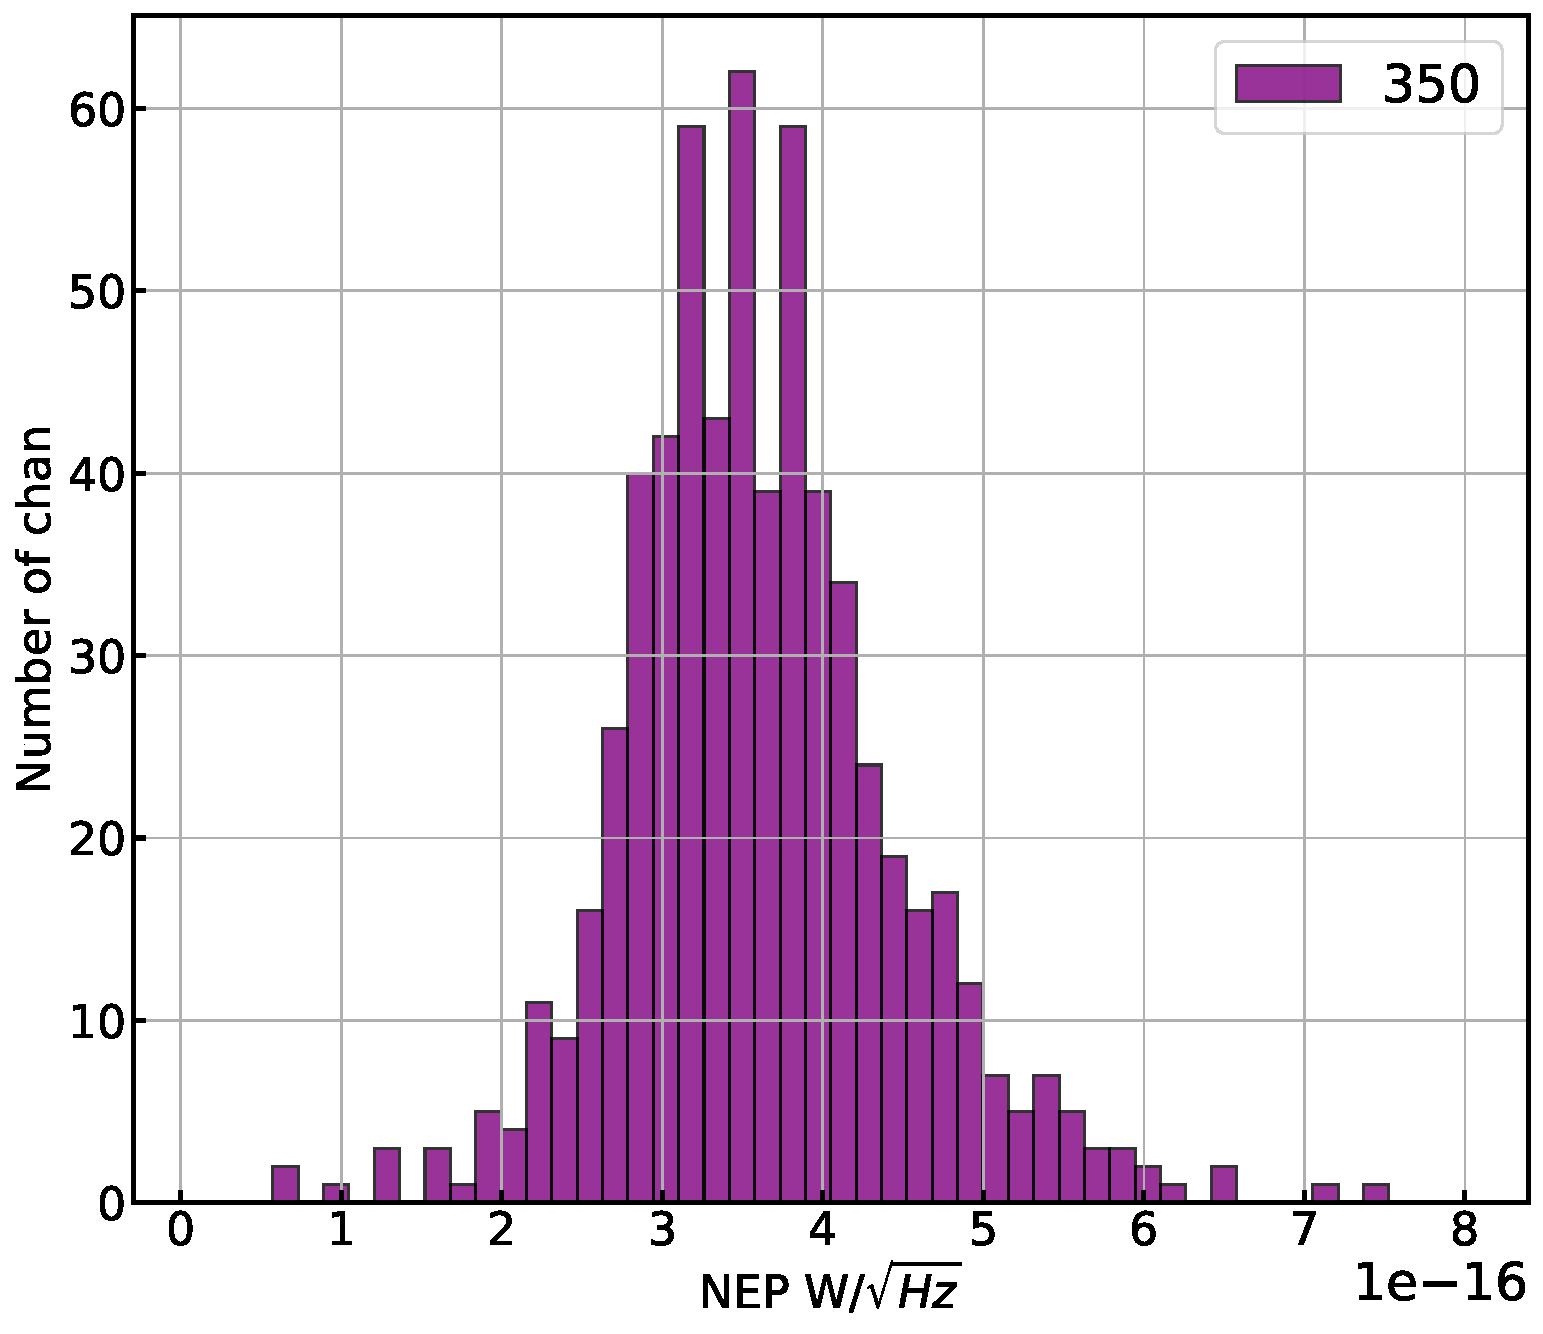
\includegraphics[width=\textwidth]{figures/blast_data/hist/PAL_NEP_hist_R3}
\caption[~Histogram of \macrocapwrap{NEP$_{\mathrm{freq}}$} for the 350~\macrocapwrap{$\upmu$m} array, measured at CSBF.]{Histogram of NEP$_{\mathrm{freq}}$ for the 350~$\upmu$m array, measured at CSBF.}
\label{fig:pal nep 350}
\end{figure}

\begin{figure}[!htbp]
\centering
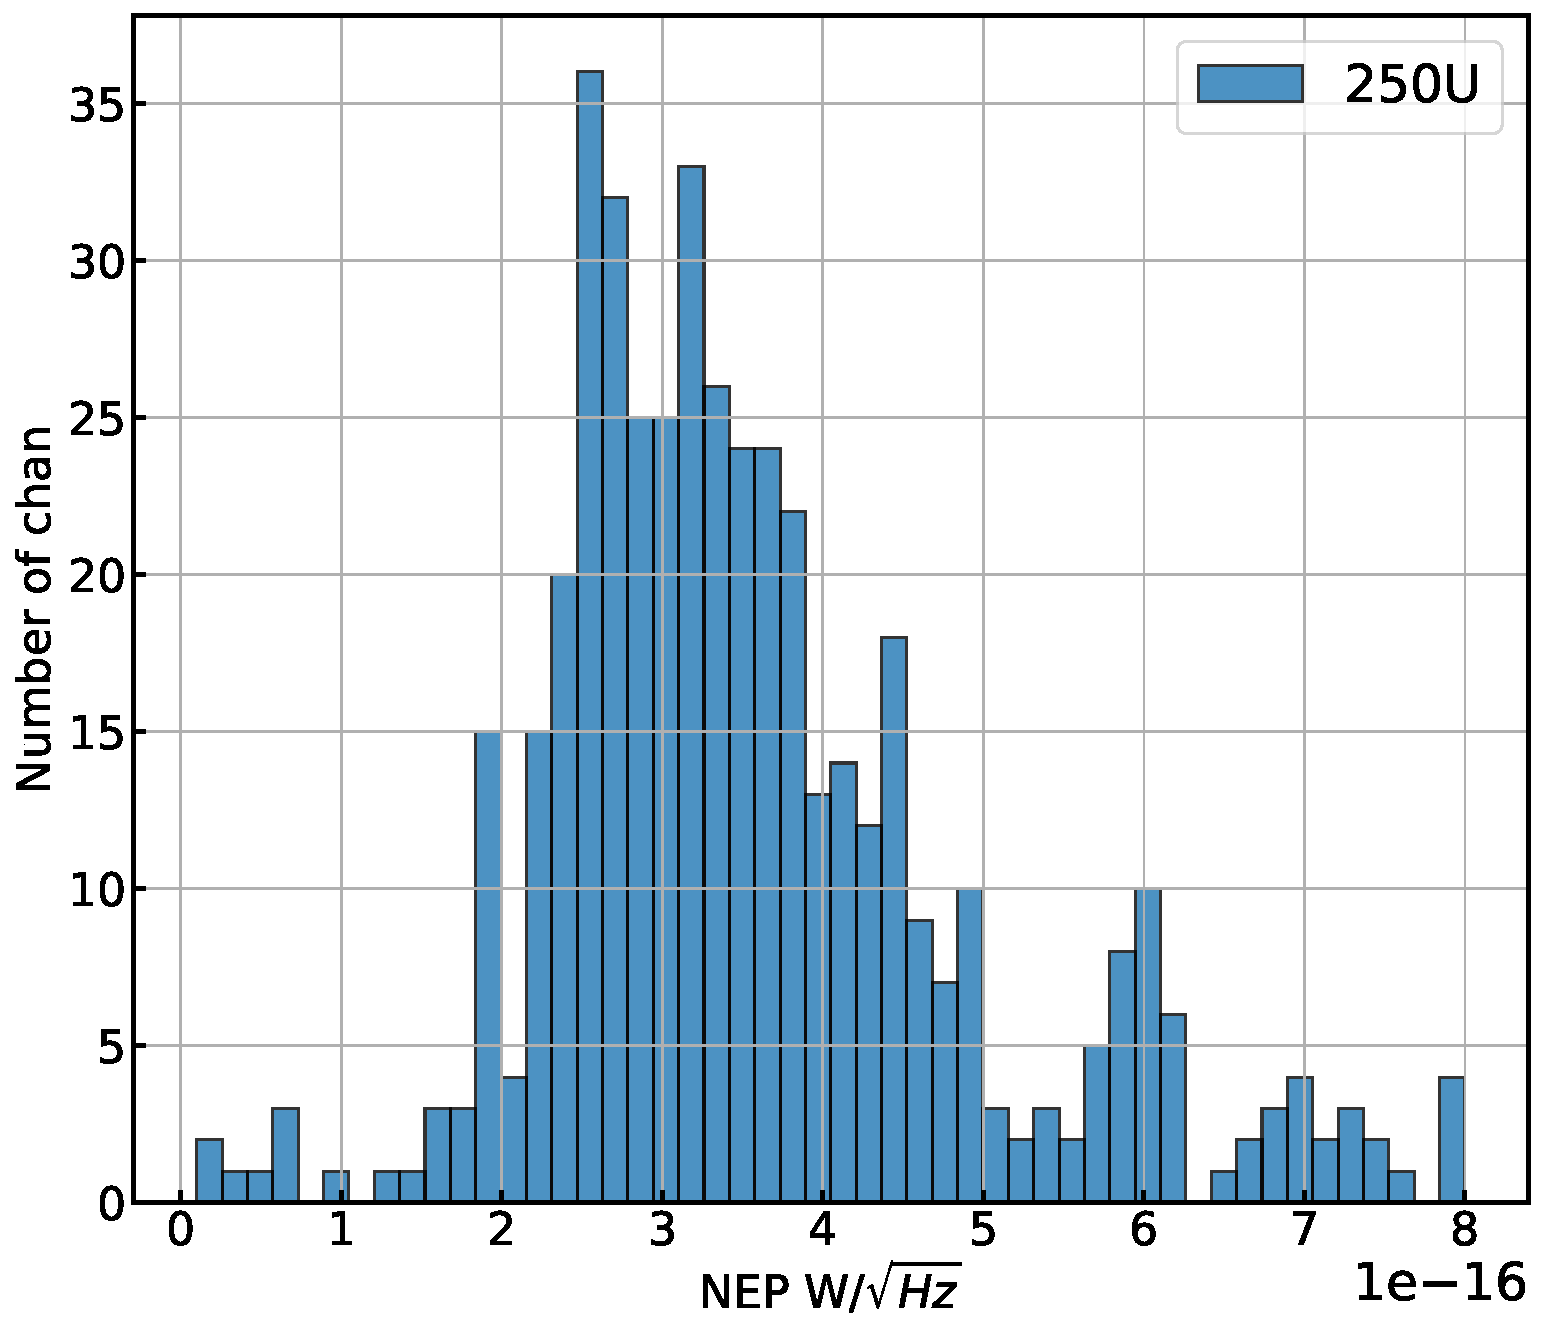
\includegraphics[width=\textwidth]{figures/blast_data/hist/PAL_NEP_hist_R4}
\caption[~Histogram of \macrocapwrap{NEP$_{\mathrm{freq}}$} for the 250U array, measured at CSBF.]{Histogram of NEP$_{\mathrm{freq}}$ for the 250U array, measured at CSBF.}
\label{fig:pal nep 250U}
\end{figure}

\begin{figure}[!htbp]
\centering
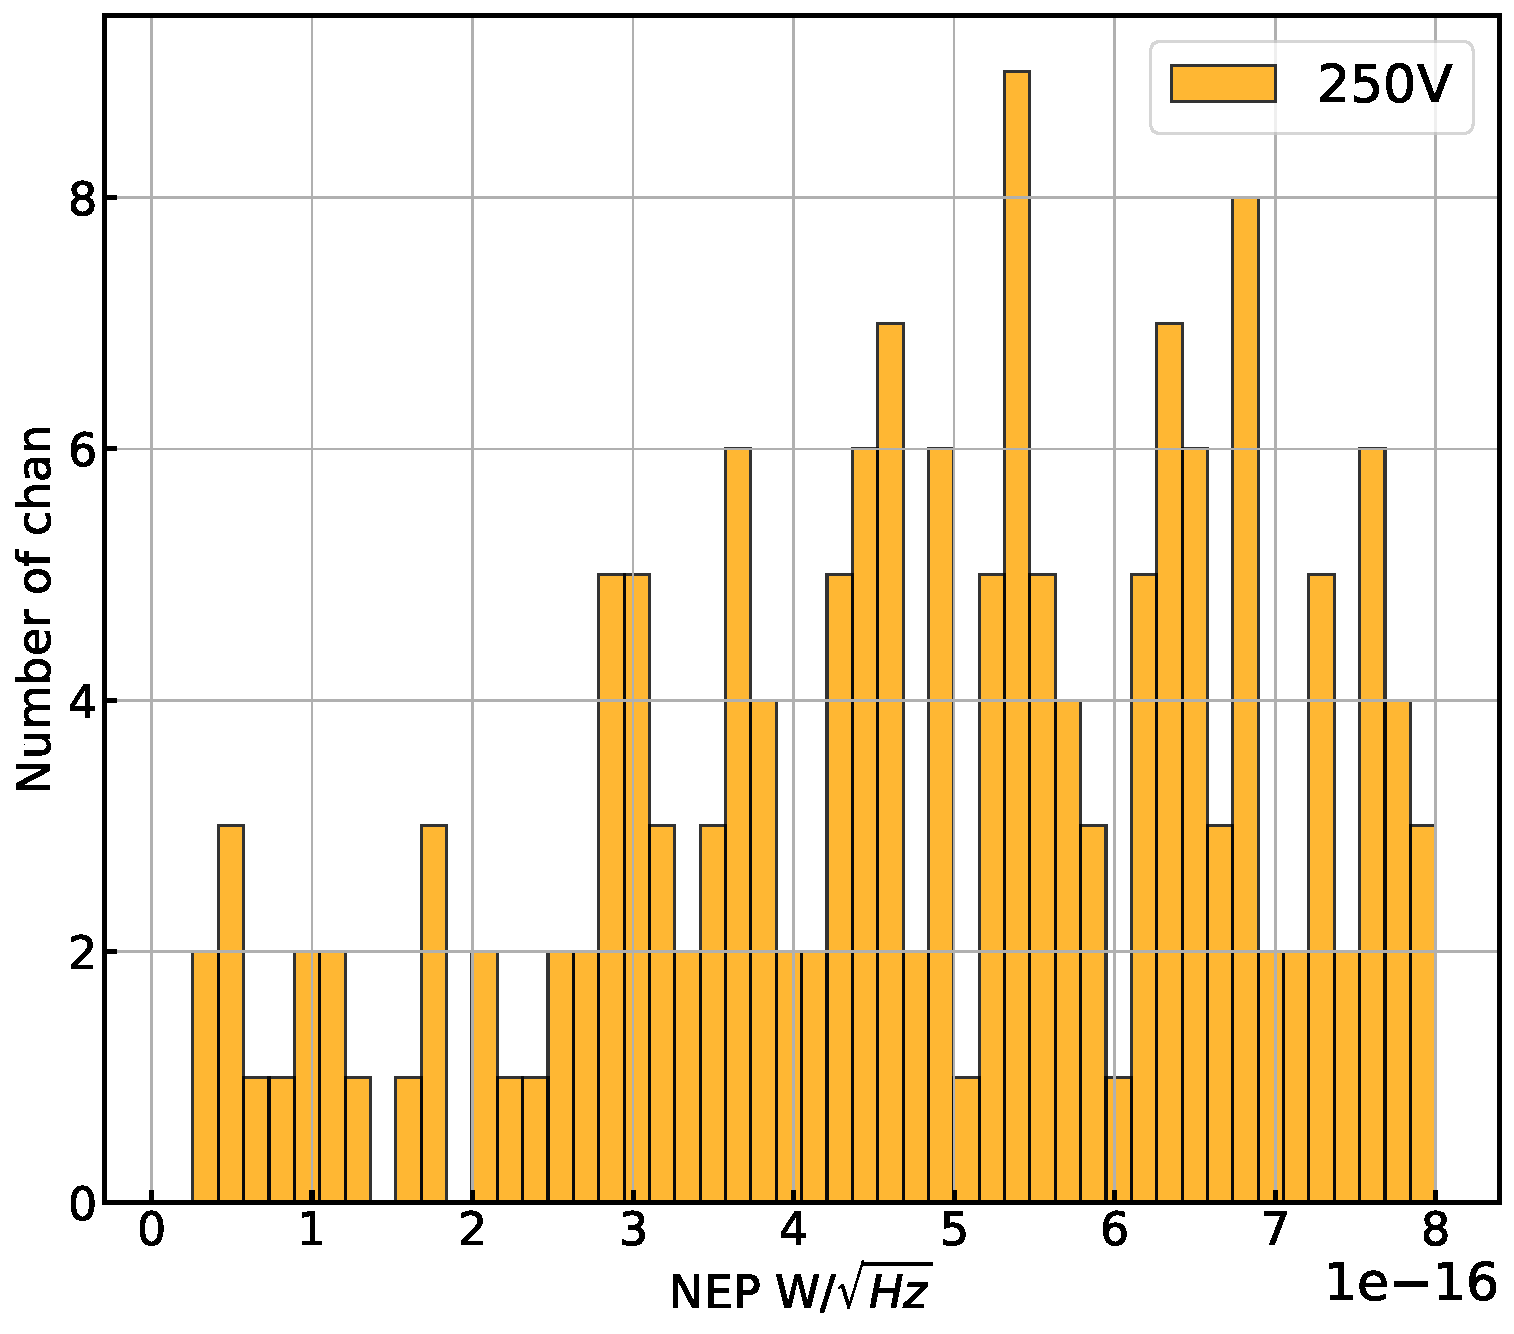
\includegraphics[width=\textwidth]{figures/blast_data/hist/PAL_NEP_hist_R2}
\caption[~Histogram of \macrocapwrap{NEP$_{\mathrm{freq}}$} for the 250V array, measured at CSBF.]{Histogram of NEP$_{\mathrm{freq}}$ for the 250V array, measured at CSBF.}
\label{fig:pal nep 250V}

\end{figure}
\begin{figure}[!htbp]
\centering
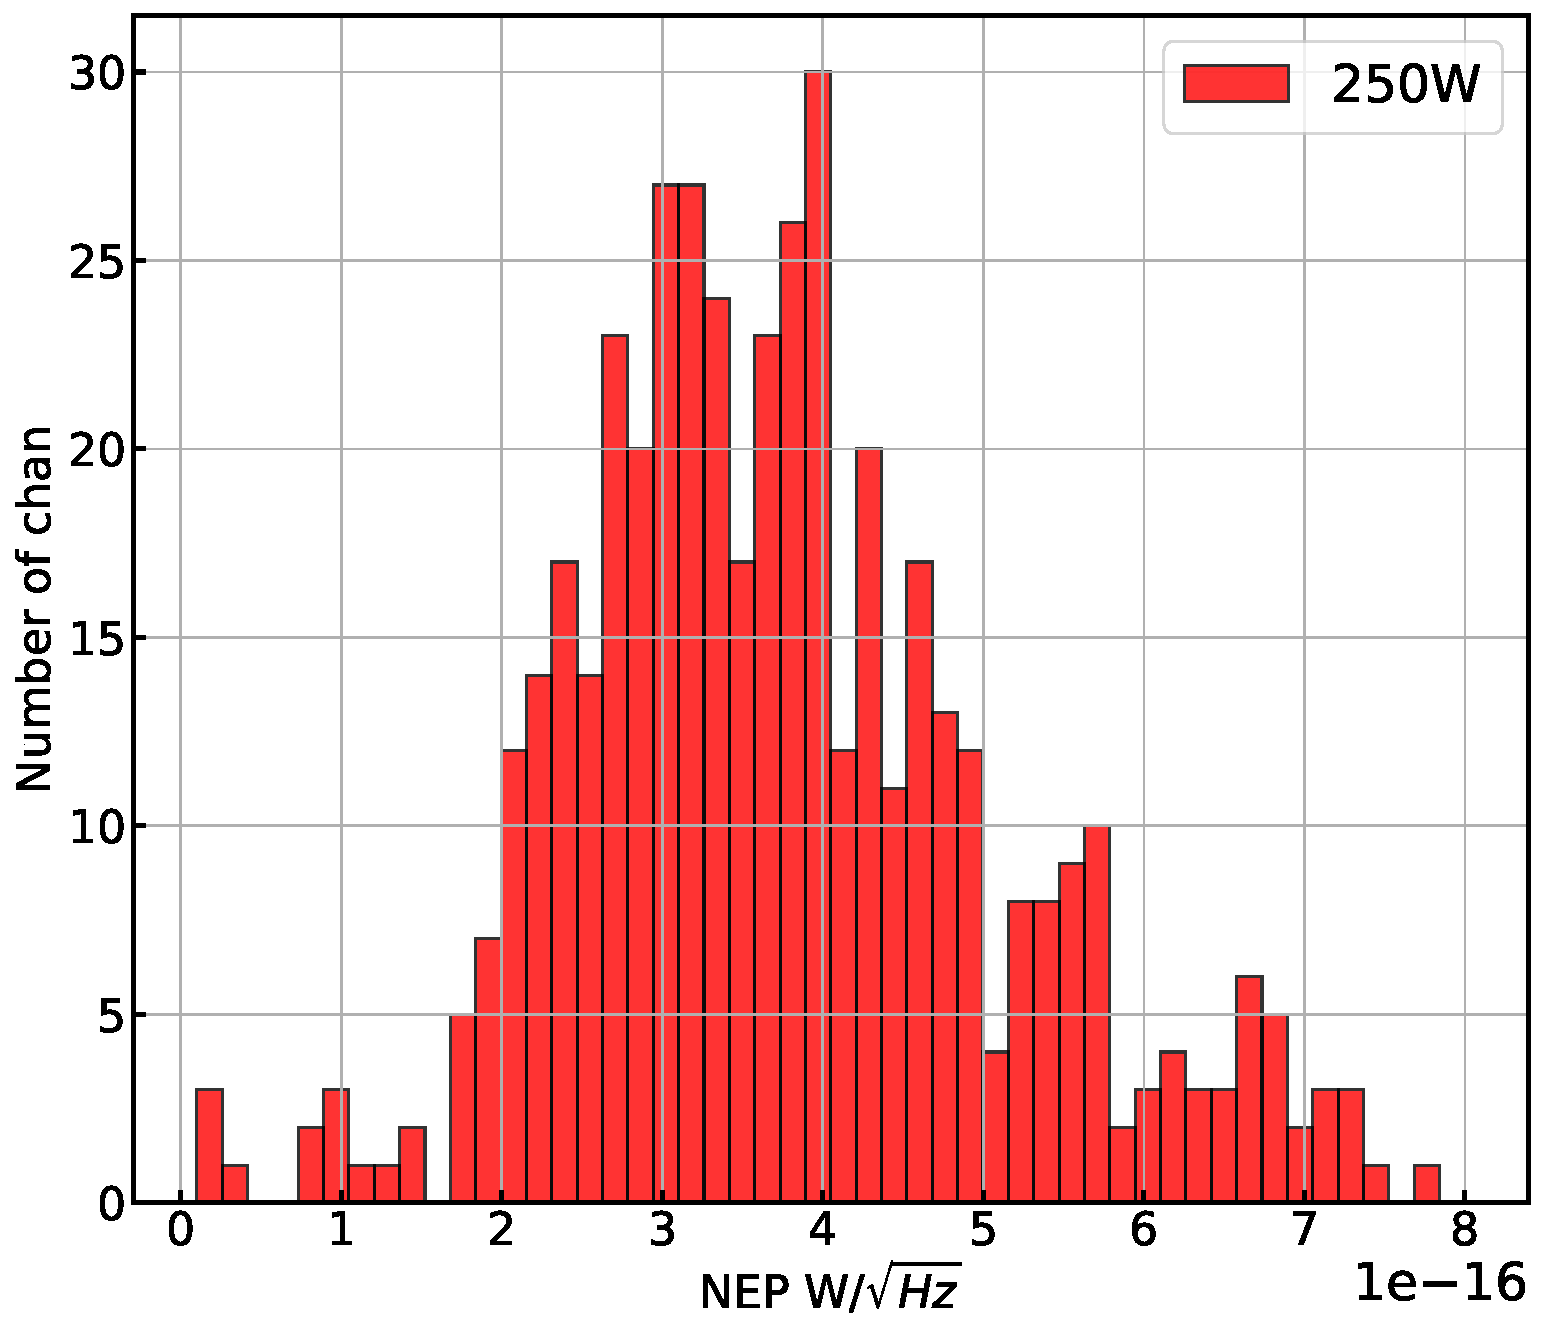
\includegraphics[width=\textwidth]{figures/blast_data/hist/PAL_NEP_hist_R5}
\caption[~Histogram of \macrocapwrap{NEP$_{\mathrm{freq}}$} for the 250W array, measured at CSBF.]{Histogram of NEP$_{\mathrm{freq}}$ for the 250W array, measured at CSBF.}
\label{fig:pal nep 250W}
\end{figure}

\section{Responsivities}\label{responsivities}

Average responsivities to absorbed optical power, $\gls{Ropt} = (df/f_{0})/\mathrm{pW}$, and to changes in base temperature, $\gls{Rtemp} = (df/f_{0})/\mathrm{mK}$, are listed in Table~\ref{table:responsivities} for the 250, 350 and 500~$\upmu$m detector arrays. The optical responsivity \gls{Ropt} is difficult to measure, because it requires the use of a well calibrated black-body source, as well as knowledge of the total optical efficiency of the detector test-bed. For the horn-coupled, polarization sensitive LEKIDs used in BLAST-TNG, the total optical efficiency includes the horn-efficiency, polarization efficiency, detector quantum efficiency and the efficiency of any optical elements, such as band-defining filters, which are present in the optical chain. Furthermore, \gls{Ropt} and \gls{Rtemp} are different for each detector. In general, either the optical efficiency of the system or the optical responsivity may be estimated by assuming a value for one or the other.

\subsection{Optical Responsivity}

In this work, we assume average values of \gls{Ropt} for each BLAST-TNG detector which were measured at NIST (shared in a communication with collaboration members). In Section~\ref{applying model}, we compare these values to those produced by the parametric LEKID model presented in Chapter 2. The BLAST-TNG receiver contains a calibration lamp which is of a similar design to the one which was used in Herschel SPIRE \citep{hargrave2006performance}. Because the absolute power output from the lamp is unknown, it is used primarily as a relative response calibrator. Examples of 1 second calibration lamp chops from CSBF and LDB are shown in Figures~\ref{fig:cal lamp pal} and Figure~\ref{fig:cal lamp ice}. The CSBF chops are shown in units of normalized \gls{phiIQ}, and represent an average over many channels. The rising edge of the pulse is visible. The chops shown in Figure~\ref{fig:cal lamp ice} are for single channels, and have been converted to \gls{df}. A low-pass filtered trace for each chop is overlayed on the raw data. Due to the lower SNR, the rising edge of the lamp pulse is not as visible.

% Cal lamp Palestine
\begin{figure}[!htbp]
\centering
\includegraphics[width=\textwidth]{figures/blast_data/timestreams/cal_lamp_chops}
\caption[~Calibration lamp chops for the 250U, 250W, 250V, 350 and 500~\macrocapwrap{$\upmu$m} arrays, taken at CSBF.]{Calibration lamp chops for the 250U, 250W, 250V, 350 and 500~$\upmu$m arrays, taken at CSBF.}
\label{fig:cal lamp pal}
\end{figure}

% Cal lamp ICE
\begin{figure}[!htbp]
\centering
\includegraphics[width=\textwidth]{figures/blast_data/timestreams/ice_lamps}
\caption[Calibration lamp chops for the 250U, 250W, 350 and 500~\macrocapwrap{$\upmu$m} arrays, taken at LDB.]{Calibration lamp chops for the 250U, 250W, 350 and 500~$\upmu$m arrays, taken at LDB.}
\label{fig:cal lamp ice}
\end{figure}

Figure~\ref{fig:T chop} shows a chop for a single channel of the 350~$\upmu$m array which was produced by chopping a thermal source in front of the cryostat window. The thermal source was at temperature of $\sim$15~K above room temperature. During this measurement, which took place in May, 2018, a 2.85\% NDF was installed in the optical chain. The top panel of Figure~\ref{fig:T chop} shows the phase quadrature of \gls{df}, and the bottom shows the dissipation quadrature. If we assume a value for either \gls{Ropt} or \gls{opt_eff}, we can estimate either an NEP or an NET for this channel. This is done in Section~\ref{sensitivity}.

% May Temperature Chop
\begin{figure}[!htbp]
\centering
\includegraphics[width=\textwidth]{figures/blast_data/timestreams/may_15K_chop_c374}
\caption[~Chops made using a \macrocapwrap{$\sim$}15~K thermal source for a single channel of the 350~\macrocapwrap{$\upmu$m} array.]{Chops made using a $\sim$15~K thermal source for a single channel of the 350~$\upmu$m array.}
\label{fig:T chop}
\end{figure}

\subsection{Base Temperature Responsivity}

At CSBF, \gls{Rtemp} was measured by taking VNA sweeps of \gls{S21} at different base temperatures. The temperatures used in this calculation are 277, 282 and 286~mK. The df/dT from the sweep was checked against values predicted by the Mattis-Bardeen theory. Figure~\ref{fig:temp sweeps} shows \gls{S21} traces for the three base temperatures are shown for a single 350~$\upmu$m resonator. The \gls{Rtemp} predicted by Mattis-Bardeen are shown in Figure~\ref{fig:temp sweeps}.

% Frequency and Temperature Responsivity
\begin{table}[!htbp]
\centering
\begin{tabular}{@{}lll@{}}
\dtoprule{}
Band & \gls{Ropt} $(df/f_{0})/\mathrm{pW}$     & \gls{Rtemp} $(df/f_{0})/\mathrm{mK}$ \\ \midrule
250~$\upmu$m & 1.7 $\times$ 10$^{-5}$ & 9.15 $\times$ 10$^{-7}$ \\
350~$\upmu$m & 5.2 $\times$ 10$^{-6}$ & 1.51 $\times$ 10$^{-6}$ \\
500~$\upmu$m & 1.6 $\times$ 10$^{-4}$ & 3.91 $\times$ 10$^{-6}$ \\ \dbottomrule{}
\\
\end{tabular}
\caption[~BLAST-TNG optical and temperature responsivities.]{BLAST-TNG optical and temperature responsivities (optical responsivities provided by NIST).}
\label{table:responsivities}
\end{table}

\begin{figure}[!htbp]
\centering
\includegraphics[width=\textwidth]{figures/blast_data/sweeps/temp_sweep_pal}
\caption[~350 \macrocapwrap{$\upmu$m} VNA sweeps at different FPA temperatures.]{350~$\upmu$m VNA $|\gls{S21}|$ sweeps at different FPA temperatures. The red trace is low-pass filtered data (Figure courtesy of Adrian Sinclair)}
\label{fig:temp sweeps}
\end{figure}

\begin{figure}[!htbp]
\centering
\includegraphics[width=\textwidth]{figures/blast_data/sweeps/temp_response}
\caption[~Mattis-Bardeen temperature responsivity curves for the 250, 350 and 500 \macrocapwrap{$\upmu$m} arrays.]{Mattis-Bardeen temperature responsivity curves for the 250, 350 and 500~$\upmu$m arrays (Figure courtesy of Adrian Sinclair).}
\label{fig:temp response}
\end{figure}

\begin{comment}
\begin{figure}[!htbp]
\centering
\includegraphics[width=\textwidth]{figures/blast_data/timestreams/May_dff0_hist}
\caption[~Mattis-Bardeen temperature responsivity curves for the 250, 350 and 500 \macrocapwrap{$\upmu$m} arrays.]{sdfsfdsf}
\label{fig:may noist hist}
\end{figure}

\begin{figure}[!htbp]
\centering
\includegraphics[width=\textwidth]{figures/blast_data/timestreams/May_350_noiseTF}
\caption[~Mattis-Bardeen temperature responsivity curves for the 250, 350 and 500 \macrocapwrap{$\upmu$m} arrays.]{sdfsfdsf}
\label{fig:may noise TRF}
\end{figure}
\end{comment}

\section{Estimating Sensitivity}\label{sensitivity}

The sensitivity of each detector is characterized by its NET, in units of $\mathrm{K}/\sqrt{\mathrm{Hz}}$, or NEP, in units of $\mathrm{W}/\sqrt{\mathrm{Hz}}$. These quantities are defined in Chapter 2. In this section, we describe how they can be estimated using the quantities introduced in previous sections.

\subsection{NET and NEP}\label{NET}

NET (or NEP) are estimated by modulating the detectors with a thermal source whose temperature relative to the background is known with some certainty. An $I/Q$ timestream of the chop is recorded for each readout channel. Without doing a frequency sweep (e.g., target or wide sweep), the NET can be calculated from the $\Delta T$ and $I/Q$ timestreams as:

% NEP from chop
\begin{equation}
  \begin{aligned}
  NET &= \Delta T \frac{e_{V}}{V_{pp}} \\
      &= \Delta T \sqrt{ \frac{ (\sigma^{2}_{I} + \sigma^{2}_{Q}) / (f_{s}/2)}{ I^{2} + Q^{2} } }  \qquad \left[ \frac{ \mathrm{K} }{ \sqrt{\mathrm{Hz}} } \right]
  \end{aligned}
\end{equation}

If the $I/Q$ timestreams are converted into units of \gls{df}, then the NET can be calculated as:

% NET from sweep and freq noise
\begin{equation}\label{eq:NET freq}
  NET = \Delta T \frac{e_{f}}{\Delta f/f_{0}} \qquad \left[ \frac{\mathrm{K}}{ \sqrt{\mathrm{Hz}} } \right]
\end{equation}

where $\Delta f$ is the size of the frequency chop, in units of Hz. The frequency noise $e_{f}$ can be calculated using either the $I/Q$ gradient method, the phase fitting method, or by fitting the resonator parameters from the sweep, as in Equation~\ref{eq:df estimate}.

If the optical responsivity is known or assumed, the NEP can be calculated as:

% NEP from R and freq noise
\begin{equation}\label{eq:NEP}
  \begin{aligned}
  NEP &= \frac{e_{f}/f_{0}}{\gls{Ropt}} \\
      &=  \frac{e_{f}/f_{0}}{(df/f_{0})/dP} \qquad \left[ \frac{\mathrm{W}}{ \sqrt{\mathrm{Hz}} } \right]
  \end{aligned}
\end{equation}

Because $e_{f}$ is complex, Equations~\ref{eq:NET freq} and~\ref{eq:NEP} allow for the NET and NEP in both the phase and dissipation quadratures to be calculated.

The thermal source chop in Figure~\ref{fig:T chop} was produced with $\Delta T \simeq 15$~K. At the time of the measurement there was a 2.85\% NDF inside the cryostat. Using Equation~\ref{eq:NET freq}, and multiplying by the loss from the NDF gives $NET_{\mathrm{tot}} = 825$~$\upmu$K/$\sqrt{\mathrm{Hz}}$. Assuming a 30\% passband width, this value corresponds to $NEP_{\mathrm{freq,tot}} = 5.55 \times 10^{-16}$~W/$\sqrt{\mathrm{Hz}}$. Assuming the \gls{Ropt} value for the 350~$\upmu$m array in Table~\ref{table:responsivities}, the optical efficiency for this channel is found to $\sim$20\%. For this particular channel, the frequency noise in the dissipation quadrature was found to be slightly less than half of the noise in the phase quadrature. This indicates that the channel is close to being photon noise limited ($NEP_{\mathrm{phot}} > NEP_{\mathrm{diss}}$, where $NEP_{\mathrm{diss}}$ is calculated using the noise in the dissipation quadrature and the frequency responsivity). Values for the NET and NEP in the two quadratures are listed in Table~\ref{table:NET NEP example}.

% NEP, thermal source chops

\begin{table}[!htbp]
\centering
\caption[~Single detector NET and NEP estimated from a thermal chop.]{Estimates of NET and NEP for a single 350~\macrocapwrap{$\upmu$m} channel. This data was recorded in May, 2018. There was a 2.85\% NDF in the optical path.}
\label{table:NET NEP example}
\begin{tabular}{@{}ll@{}}
\dtoprule{}
 & Channel 618 \\ \midrule
$f_{0}$ MHz & 668.44 \\
\gls{Sxx} Hz$^{-1}$ & 8.34 $\times$ 10$^{-18}$ \\
\gls{Syy} Hz$^{-1}$ & 3.99 $\times$ 10$^{-18}$ \\
NEP$_{\mathrm{freq}}$ W/$\sqrt{\mathrm{Hz}}$ & 5.55 $\times$ 10$^{-16}$ \\
NEP$_{\mathrm{diss}}$ W/$\sqrt{\mathrm{Hz}}$ & 3.84 $\times$ 10$^{-16}$ \\
NET$_{\mathrm{freq}}$ $\upmu$K/$\sqrt{\mathrm{Hz}}$ & 825 \\
NET$_{\mathrm{diss}}$ $\upmu$K/$\sqrt{\mathrm{Hz}}$ & 571 \\
NDF & 0.0285 \\
\gls{opt_eff} (estimated) & 0.19 \\ \dbottomrule{}
\\
\end{tabular}
\end{table}

\subsection{NEFD and Mapping Speed}\label{nefd}

To relate NEP to mapping speed, it is useful to convert it into a Noise-equivalent flux density (NEFD). For sub-mm astronomical instruments, NEFD is typically reported in units of $\mathrm{MJy}/\sqrt{\mathrm{Hz}}$ or $\mathrm{MJy}\sqrt{\mathrm{s}}$ (1 Jy = 10$^{-26}$~W/m$^{2}$Hz). Here, we convert the median eletrical NEP values measured for each BLAST-TNG detector array (see Section~\ref{histograms}) into NEFD, and then into a per-beam RMS noise level for each waveband, $\sigma_{\mathrm{map}}$, in units of mJy/beam. The conversion from NEP in $\mathrm{W}/\sqrt{\mathrm{Hz}}$ to NEFD in $\mathrm{MJy}\sqrt{\mathrm{s}}$ is done as:

\begin{equation}\label{eq:nep to nefd}
  NEFD = \sqrt{0.5} 10^{-20} \frac{NEP}{A_{\mathrm{beam}} B_{\mathrm{opt}}} \qquad \left[ \frac{\mathrm{MJy}\sqrt{\mathrm{s}}}{ \mathrm{sr} } \right]
\end{equation}

where the factor of $\sqrt{0.5}$ accounts for the conversion from 1/$\sqrt{\mathrm{Hz}}$ to $\sqrt{\mathrm{s}}$, $A_{\mathrm{beam}}$ is the beam area in steradians and $B_{\mathrm{opt}}$ is the optical bandwidth. Table~\ref{table:NEP comparison} compares the NEPs and NEFD measured in Palestine for each array to the total (phase quadrature) and photon NEPs listed in the original BLAST-TNG proposal. $I_{\mathrm{min}}$ is the source intensity which would be needed to measure 1-$\sigma$ error bars on the polarization fraction of 0.5\% over a 1 deg$^{2}$ area after a 5~hour integration (this quantity is discussed in Chapter 5). Values for the map noise $\sigma_{\mathrm{map}}$ is shown per-detector, as well as accounting for the total number of detectors in each band. The NEFD which is given accounts for the total number of detectors.

% NEP proposal v. measured NEP
\begin{table}[!htbp]
  \begin{threeparttable}
\centering
\caption{NEP and NEFD estimates from Palestine tests, compared to proposal values.}
\label{table:NEP comparison}
\begin{tabular}{@{}llll@{}}
\dtoprule{}
 & 250~$\upmu$m & 350~$\upmu$m & 500~$\upmu$m \\ \midrule
NEP$_{\mathrm{freq,prop}}$\tnote{1} W/$\sqrt{\mathrm{Hz}}$ & 6.5 $\times$ 10$^{-17}$ & 5.5 $\times$ 10$^{-17}$ & 4.7 $\times$ 10$^{-17}$ \\
NEP$_{\mathrm{phot,prop}}$ W/$\sqrt{\mathrm{Hz}}$ & 17 $\times$ 10$^{-17}$ & 12 $\times$ 10$^{-17}$ & 8.7 $\times$ 10$^{-17}$ \\
NEP$_{\mathrm{freq,Pal}}$ W/$\sqrt{\mathrm{Hz}}$ & 35 $\times$ 10$^{-17}$ & 35 $\times$ 10$^{-17}$ & 10.0 $\times$ 10$^{-17}$ \\
NEFD$_{\mathrm{PAL}}$ $\frac{MJy\sqrt{s}}{sr}$ & 0.13 & 0.12 & 0.034 \\
$\sigma_{\mathrm{map}}$ mJy/beam per detector & 68.75 & 96.25 & 39.28 \\
$\sigma_{\mathrm{map}}$ mJy/beam & 2.17 & 3.77 & 2.27 \\
$I_{\mathrm{min}}$ MJy/sr & 78.16 & 49.46 & 10.19 \\ \dbottomrule{}
\\
\end{tabular}
\begin{tablenotes}
\item [1] Values from the original BLAST-TNG proposal.
\vspace{2mm}
\end{tablenotes}
\end{threeparttable}
\end{table}

The measured electrical NEP values from Palestine are slightly higher than the estimated values in the proposal, but comparable to those given for the photon noise NEPs in the proposal. During the measurement when the electrical NEPs were calculated, it is possible that many of the detectors were photon noise limited. However, they were not optimally biased in terms of readout power, which causes the NEP in the dissipation direction to contribute more to the total NEP\@. The values for NEP$_{\mathrm{freq}}$ given in the proposal assume that the dissipation quadrature contributes $\sim$33\% to the total. In the Palestine measurements, the dissipation quadrature constitutes $\sim$65\% of the total.

Despite the slightly higher NEPs, the NEFDs are lower than in BLAST 2006 and the corresponding mapping speed is an order of magnitude higher \citep{marsden2009blast}. This bodes well for the planned 2019/2020 flight of BLAST-TNG\@.

%%%%%%%%%%%%%%%%%%%%%%%%%%%%%%%%%%%%%%%%%%%%%%%%%%%%%%%%%%%%%%%%%%%%%%%
% Model fitting
\section{Applying the LEKID Model to Measured Data}\label{applying model}

In this section we apply the parametric LEKID model which was developed in Chapter 2 to measured data from the 2018--2019 Antarctic campaign to determine whether or not it can provide reasonable estimates of absorbed optical power and optical efficiency for a single resonator. During pre-flight preparations at LDB, no NDF was installed inside the receiver, and the detectors were exposed to the ambient $\sim$290~K loading from the highbay. Despite their being heavily loaded, the majority of the detectors still responded to calibration lamp pulses.

At the end of the ice campaign, data was taken with the aluminum camera shutter in the open and closed states. The shutter blocks the optical path between the primary mirror and the cryostat window, and is used during ascent when there is a risk of exposing the detectors to direct sunlight due to uncontrolled pointing. The WiFi and star-camera video transmitter were powered down during this test, since they had been previously been discovered to interfere with the detector timestreams.

As a test of the model, we choose a single channel from the 350~$\upmu$m array. The model takes \gls{Pro}, \gls{Tbase}, \gls{Popt}, $f_{0}$, \gls{Qc}, $Q_{\mathrm{loss}}$ and $\epsilon_{assym}$ as inputs. To simulate the test channel, we begin by estimating these and other resonator parameters using the target sweep and $I/Q$ timestreams taken in the shutter-closed and shutter-open states. The estimated parameters, listed in Table~\ref{table:350 model}, include: $f_{0}$, \gls{Qr}, \gls{Qc}, dip-depth, \gls{asym}, $\gls{Sxx}$, $NEP_{\mathrm{freq}}$ and $NEP_{\mathrm{diss}}$. For \gls{Tbase} we assume 287~mK, which was the temperature of the 350~$\upmu$m focal-plane-array at the time that the data was recorded. For \gls{Popt} we use the range between 1--200~pW, divided into 500 intervals. The readout power \gls{Pro} is -83~dBm.

\subsection{Optical Response}

Given the inputs listed above, the model returns \gls{S21}(\gls{Popt}) for each optical power in the input range. A fit of \gls{S21} to both the shutter-closed and shutter-open data is shown in Figure~\ref{fig:350 S21 model}. The measured data is shown as blue points, the initial fit is shown as a dashed black line, and the model fit is shown as a dashed red line. To produce the model traces shown in Figure~\ref{fig:350 S21 model}, we select the two \gls{S21}(\gls{Popt}) arrays which correspond to the $f_{0,\mathrm{closed}}$ and $f_{0,\mathrm{open}}$ values determined from the initial fit. To create a good fit to \gls{S21}, we find that we must add a frequency offset to the value of $f_{0}$ which is input to the model. For this test, we find that a frequency offset of 110~kHz produces good results. The resonator quality factors produced by the parametric model (listed in Table~\ref{table:350 model}) match those of the initial fit to within a few percent.

The frequency shift between the two resonator states is -95.47~kHz. Using this shift, the model can be used to estimate the optical responsivity \gls{Ropt}. The responsivity is sensitive to the value which is chosen for \gls{N0}, the single-spin density of states at the Fermi Energy. Using $\gls{N0} = 10^{10}$~$\mathrm{eV}^{-1}$~$\upmu$m$^{3}$, the model reports \gls{Ropt} = 5.35~pW$^{-1}$. This value is close to the average \gls{Ropt} reported by NIST, which is listed in Table~\ref{table:responsivities}. Given the frequency shift and responsivity, the power absorbed by the resonator between the two states is $\Delta \gls{Pabs} \approx 22$~pW.

\begin{table}[!htbp]
  \begin{threeparttable}
\centering
\caption{350 \macrocapwrap{$\upmu$m} model parameters.}
\label{table:350 model}
\begin{tabular}{@{}lllll@{}}
\dtoprule{}
 & \begin{tabular}[c]{@{}l@{}}Shutter closed\\ (est.\ from data)\end{tabular} & \begin{tabular}[c]{@{}l@{}}Shutter open\\ (est.\ from data)\end{tabular} & \begin{tabular}[c]{@{}l@{}}Shutter closed\\ (model)\end{tabular} & \begin{tabular}[c]{@{}l@{}}Shutter open\\ (model)\end{tabular} \\ \midrule
$f_{0}$ (MHz) & 813.330 & 813.235 & 813.330 & 813.235 \\
\gls{Qr} & 15,829 & 12,106 & 15,600 & 11,724 \\
\gls{Qc} & 25,328 & 24216 &  &  \\
\gls{Qi} & 42,316 & 24,246 & 40,615 & 21,829 \\
depth (dB) & -8.42 & -5.77 & -8.31 & -5.40 \\
\gls{asym} & -0.20 & -0.28 &  &  \\
R$_{P, \mathrm{model}}$ (1/pW) & 5.35 $\times$ 10$^{-6}$ &  &  &  \\
NEP$_{\mathrm{freq}}$ W/$\sqrt{\mathrm{Hz}}$ & 4.87 $\times$ 10$^{-16}$ & 7.11 $\times$ 10$^{-16}$ & 4.88 $\times$ 10$^{-16}$ & 7.11 $\times$ 10$^{-16}$ \\
NEP$_{\mathrm{diss}}$ W/$\sqrt{\mathrm{Hz}}$ & 4.06 $\times$ 10$^{-16}$ & 6.40 $\times$ 10$^{-16}$ &  &  \\
NEP$_{\mathrm{phot}}$ W/$\sqrt{\mathrm{Hz}}$ &  &  & 3.99 $\times$ 10$^{-16}$ & 5.33 $\times$ 10$^{-16}$ \\
NEP$_{\mathrm{amp}}$ W/$\sqrt{\mathrm{Hz}}$ &  &  & 2.34 $\times$ 10$^{-16}$ & 4.32 $\times$ 10$^{-16}$ \\
$\gls{Sxx}$ (1/Hz) & 6.80 $\times$ 10$^{-18}$ & 1.45 $\times$ 10$^{-17}$ & 6.83 $\times$ 10$^{-18}$   &  1.45 $\times$ 10$^{-17}$ \\
$S_{YY}$ (1/Hz) & 4.72 $\times$ 10$^{-18}$ & 1.17 $\times$ 10$^{-17}$     &       &    \\
$\Delta \gls{Pabs}$ (pW) &  & 22 &  & 22 (58) \\
\gls{Pabs}(pW) &  &  & 103 & 161 \\
T$_{\mathrm{shutter}}$ (K) &  &  &  & 250 \\
\gls{opt_eff} &  &  &  & 0.28 \\
$Q_{\mathrm{loss}}$  & 3 $\times$ 10$^{7}$ & & & \\
\gls{N0} $\mathrm{eV}^{-1}$~$\upmu$m$^{3}$ & 9.5 $\times$ 10$^{10}$ &  &  &  \\ \dbottomrule{}
\\
\end{tabular}
\end{threeparttable}
\end{table}

Next, we compare the measured values for fractional frequency noise $\gls{Sxx}$, and NEP, to the values produced by the model. Because of the frequency offset which was applied to the $f_{0}$ values in order to obtain a good \gls{S21} fit, we do not use the values for $\gls{Sxx}$ and NEP which correspond to those traces. Instead, we locate the two \gls{S21}(\gls{Popt}) traces that have a fractional frequency noise $\gls{Sxx}$ (1/Hz) which is closest to the values of $\gls{Sxx}$ which are estimated from the data. The two \gls{S21} traces which are found to match the closed and open states have $f_{0}$ values which are offset by those of the original \gls{S21} traces by -413 and -566~kHz, respectively. At the time of writing, the source of this frequency offset is not understood. Apart from the frequency offset, the frequency noise and NEP values produced by the model are close matches to the measured values.

Table~\ref{table:350 model} lists the measured values for $\gls{Sxx}$, $S_{YY}$, NEP$_{\mathrm{freq}}$ and NEP$_{\mathrm{diss}}$ in the shutter-open and shutter-closed states. Figure~\ref{fig:350 chan psd} shows the fractional frequency power spectral density for the measured $\gls{Sxx}$ and $S_{YY}$. The black line indicates the white noise level which corresponds to their difference. Because the measured value for $\gls{Sxx}$ was used to select the appropriate \gls{S21} array, the measured and model values for $\gls{Sxx}$ and NEP$_{\mathrm{freq}}$ values in Table~\ref{table:350 model} agree to within a fraction of a percent.

The model \gls{S21} traces with total frequency noise that matches the measured noise correspond to optical powers of 161 and 103~pW, for the open and closed states. The ratio of these powers is 1.55, which is close to the measured ratio of NEP$_{\mathrm{freq}}$ between the closed and open states (1.50). Figure~\ref{fig:nep ratio} shows the predicted ratio of NEP$_{\mathrm{phot}}$ to NEP$_{\mathrm{amp}}$ as a function of optical power. At the optical powers corresponding to the open and closed states, these ratios equal 1.23 and 1.7, which indicate that the detector is photon noise limited. However, the value of the optical power given by the model does not necessarily equate to the true optical power (despite being close to what would be expected for an optical efficiency of $\sim$20\%.)

To estimate the system optical efficiency \gls{opt_eff}, we start by assuming that with the shutter open and without an NDF inside the cryostat, the detectors see an optical load of $\sim$290~K. Assuming a detector efficiency \gls{det_eff} of 80\%, a horn efficiency $\gamma_{\mathrm{horn}}$ of 70\% and a 30\% optical passband centered on 350~$\upmu$m, the total power incident on the detectors is:

\begin{equation}\label{eq:opt eff}
  \gls{Popt} \simeq k T B_{\mathrm{opt}} \gls{det_eff} \eta_{\mathrm{horn}}
\end{equation}

Assuming the above values, $\gls{Popt} \simeq 576$~pW. Assuming the model value of $\Delta \gls{Pabs} = 161$~pW which is based on the measured frequency noise, $\gls{opt_eff} \sim 28$\%. Given the design target value of 30\%, this estimate is reasonable. However, there is a discrepancy between the model's prediction of $\Delta \gls{Pabs}\approx 22$~pW and the difference in absorbed power between the shutter-open and closed states of $\sim$58~pW which is based on the measured frequency noise. It is unclear whether this discrepancy originates in the model or in the measured data. Because the model responsivity is very close to the responsivity reported by NIST, for the purposes of this test we assume that the discrepancy originates in the model, and disregard the value it reports for $\gls{Pabs}$ in the closed state. Assuming the model values for $\Delta \gls{Pabs}$ and $\gls{opt_eff}$, the shutter temperature is estimated as $\sim$250~K.

\begin{figure}[!htbp]
\centering
\includegraphics[width=\textwidth]{figures/blast_data/sweeps/350_S21model_ice_final}
\caption[~A parametric fit of \macrocapwrap{\gls{S21}} for an optically shifted 350~\macrocapwrap{$\upmu$m} channel.]{A fit to \gls{S21} for an optically shifted 350~$\upmu$m channel using the parametric LEKID model presented in Chapter 2 (red). The blue points are measured data.}
\label{fig:350 S21 model}
\end{figure}

\begin{figure}[!htbp]
\centering
\includegraphics[width=\textwidth]{figures/blast_data/sweeps/350_NEPphotNEPamp}
\caption[~Model ratio of \macrocapwrap{$NEP_{\mathrm{phot}}$} to \macrocapwrap{$NEP_{\mathrm{amp}}$} for a  350~\macrocapwrap{$\upmu$m} channel.]{The ratio of $NEP_{\mathrm{phot}}$ to $NEP_{\mathrm{amp}}$ for a 350~$\upmu$m channel.}
\label{fig:nep ratio}
\end{figure}

\begin{figure}[!htbp]
\centering
\includegraphics[width=\textwidth]{figures/blast_data/sweeps/350_model_psds}
\caption[~Fractional frequency noise for the camera shutter open and closed.]{The measured fractional frequency noise $\gls{Sxx}$ for the 350~$\upmu$m channel, with the camera shutter open and closed.}
\label{fig:350 chan psd}
\end{figure}

%%%%%%%%%%%%%%%%%%%%%%%%%%%%%%%%%%%%%%%%%%
% Temperature fitting
%%%%%%%%%%%%%%%%%%%%%%%%%%%%%%%%%%%%%%%%%%%

\subsection{Temperature Response}

The parametric model can also be used to estimate the responsivity to changes in base-temperature, \gls{Rtemp}. After recording data with the shutter open and closed, it was left closed while the base-temperature of the cryostat was raised. Wide and target sweeps were taken at $\gls{Tbase} \approx 287$~mK and 316~mK. The model fit to $\gls{S21}(\gls{Tbase})$ at both temperatures is shown in Figure~\ref{fig:S21 model T shift ice}. As with the optical responsivity model fit, we use $\gls{Sxx}$ to estimate the \gls{Tbase}, and the frequency shift between states to estimate the responsivity. The results of the fit are listed in Table~\ref{table:350 temp model}.

The fits to the base-temperatures are within 4~K of the temperatures which were measured using the cryogenic thermometry. The \gls{Rtemp} value measured from the frequency shift of 32~kHz is 1.4 $\times$ 10$^{-7}$. This value is lower than the \gls{Rtemp} of 9.15 $\times$ 10$^{-7}$ which was measured during the Palestine integration, but the difference is reasonable given that we are comparing two different channels under different conditions.

\begin{table}[!htbp]
\centering
\begin{tabular}{@{}llllll@{}}
\dtoprule{}
\begin{tabular}[c]{@{}l@{}}$f_{0,\mathrm{\mathrm{cold}}}$\\ (MHz)\end{tabular} & \begin{tabular}[c]{@{}l@{}}$f_{0,\mathrm{\mathrm{warm}}}$\\ (MHz)\end{tabular} & \begin{tabular}[c]{@{}l@{}}$T_{\mathrm{warm}}$ \\ (meas,mod) mK \end{tabular} & \begin{tabular}[c]{@{}l@{}}$T_{\mathrm{cold}}$ \\ (meas,mod) mK \end{tabular} & \begin{tabular}[c]{@{}l@{}}$(df/f_{0})/dT$ meas.\\ (K$^{-1}$)\end{tabular} & \begin{tabular}[c]{@{}l@{}}$(df/f_{0})/dT$ mod.\\ (K$^{-1}$)\end{tabular} \\ \midrule
813.328 & 813.298 & 316, 311 & 287, 283 & 1.35 $\times$ 10$^{-7}$ & 1.40 $\times$ 10$^{-7}$ \\ \dbottomrule{}
\end{tabular}
\caption[~Model and measured parameters for the 350~\macrocapwrap{$\upmu$m} base temperature response.]{Model and measured parameters for the 350~$\upmu$m base temperature response.}
\label{table:350 temp model}
\end{table}

\begin{figure}[!htbp]
\centering
\includegraphics[width=\textwidth]{figures/blast_data/sweeps/350_S21modelT_ice}
\caption[~A parametric fit of \macrocapwrap{$\gls{S21}(\gls{Tbase})$} for a base-temperature shifted 350~\macrocapwrap{$\upmu$m} channel.]{A fit to $\gls{S21}(\gls{Tbase})$ for a temperature shifted 350~$\upmu$m channel using the parametric LEKID model presented in Chapter 2 (red). The blue points are measured data.}
\label{fig:S21 model T shift ice}
\end{figure}

\section{Optical Tests}\label{optical tests}

The following sections describe the passband mapping and polarization efficiency tests that were performed in the lead-up to the planned 2018/2019 Antarctic flight of BLAST-TNG\@.

\subsection{Passband Mapping}\label{fts}

In this section we describe the characterization of the camera's spectral passbands. The low-frequency edge of each BLAST-TNG waveband is defined by the horn array waveguide cutoff frequencies, and the high frequency edges are defined by low-pass edge (LPE) and dichroic filters. Ideally, the passbands should be three boxcar filters centered at 250~$\upmu$m, 350~$\upmu$m and 500~$\upmu$m. Their widths should be $\sim$30\% of each center frequency (360~GHz, 257~GHz and 180~GHz). In practice, the filter shapes will not be rectangular. Their shape will be the product of the filter responses of each component in the optical path of the instrument.

A Fourier-transform spectrometer (FTS) containing a water-cooled mercury arc lamp was used to produce in-band emission over the three wavebands. A low-pass filter inside the FTS prevents high frequency photons from exiting the output aperture. During the measurement, the FTS aperture was positioned a few inches in front of the cryostat window, to ensure that the in-band source filled the entire beam. The setup in the CSBF highbay is shown in Figure~\ref{fig:fts setup}.

\begin{figure}[!htbp]
\centering
\includegraphics[width=\textwidth]{figures/blast_data/fts/fts_setup}
\caption{The FTS measurement setup at CSBF.}
\label{fig:fts setup}
\end{figure}

A FTS is a modified Michelson interferometer. A single beam of light is split into two paths by a beamsplitter. The two beams then reflect off of mirrors which send them back through the beamsplitter to recombine. In an FTS, one of the mirrors can be translated back and forth through a distance $\Delta L$ to create a variable optical path-length delay (OPD) between the two optical paths. At the output of the FTS, the intensity at optical frequency $\nu$ for a given OPD is:

% Intensity for single wavenumber and path length difference
\begin{equation}
  I(\nu, \Delta L) = I(\nu, 0) \left[1 + \cos(2\pi \nu (2 \Delta L))\right]
\end{equation}

where $I(\nu)_{\mathrm{ZPD}}$ is the intensity corresponding to the zero-path length difference (ZPD). Summing the intensities over all frequencies within the waveband gives:

% Fourier cosine transform
\begin{equation}\label{eq:FTS}
  I(\Delta L) = \int_{\nu_{0}}^{\nu_{1}} I(\nu, \Delta L) d\nu
\end{equation}

Equation~\ref{eq:FTS} is the Fourier cosine transform (real Fourier-transform). As the movable mirror inside the FTS is stepped through $\Delta L$, the recorded timestream for each channel is an interference pattern called an interferogram. Each point in the interferogram corresponds to Equation~\ref{eq:FTS} for a given path-length difference $\Delta L$, and therefore contains information about the intensity of every optical frequency in the waveband. The desired passband spectrum is produced by taking the inverse Fourier-transform of Equation~\ref{eq:FTS}, $\mathcal{F}^{-1}(I(\Delta L))$, and then shifting the Fourier frequencies into the optical band (see Equation~\ref{eq:fts scale}). The resulting frequency resolution of the spectrum $\nu_{\mathrm{res}}$ depends only on the OPD\@: $\nu_{\mathrm{res}} = c/2 \Delta L$.

The FTS measurement parameters are shown in Table~\ref{table:fts params}.

\begin{table}[!htbp]
\caption[~FTS measurement parameters.]{FTS measurement parameters.}
  \centering
\begin{threeparttable}
\begin{tabular}{@{}ll@{}}
\dtoprule{}
Parameter & Value \\ \midrule
$\Delta L$ (mm) & 100 \\
v$_{\mathrm{mirror}}$ (mm/s) & 0.1 \\
f$_{s}$ (Hz) & 488.28125 \\
f$_{c}$\tnote{1} (Hz) & 3 \\
N$_{\mathrm{samp}}$ & 4 $\times$ 10$^{4}$ \\
$\nu_{\mathrm{res}}$ (GHz) & 1.5 \\
f$_{\mathrm{scale}}$ (GHz) & 1.22 $\times$ 10$^{14}$ \\ \dbottomrule{}
\end{tabular}
\begin{tablenotes}
\item [1] cutoff frequency of the low-pass filter used to process interferograms.
\vspace{2mm}
\end{tablenotes}
\label{table:fts params}
\end{threeparttable}
\end{table}

In the following, we describe each step of the FTS data reduction for the 250W, 350~$\upmu$m and 500~$\upmu$m detector arrays. The measurement lasted $\sim$5.5 hours, during which $\sim$40 min of data was recorded for each BLAST-TNG detector with the FTS positioned in five different orientations relative to the cryostat window-- centered, above-center, below-center, right-of-center and left-of-center. These positions were used to maximize the likelihood that the beam for each detector channel would be well illuminated in at least one of the positions. Figure~\ref{fig:fts total meas} shows a phase timestream of the entire measurement for a single channel of the 350~$\upmu$m array. Due to slow drifts in the fridge temperature, the readout tones had to be recalibrated three times during the measurement (visible as large spikes). The features between $\sim$1--1.1 $\times$ 10$^{7}$ samples correspond to the cryogenic pumped-pot running out of He4, and then refilling.

\begin{figure}[!htbp]
\centering
\includegraphics[width=\textwidth]{figures/blast_data/fts/fts_long_raw}
\caption[The timestream of the FTS measurement, for a single channel of the \macrocapwrap{350~$\upmu$m} array.]{The timestream of the FTS measurement, for a single channel of the 350~$\upmu$m array. The measurement duration is $\sim$5.5~hours.}
\label{fig:fts total meas}
\end{figure}

The data reduction steps used to create the passband spectrum spectrum for each band (shown in Figure~\ref{fig:passbands_corr}) are:

\begin{enumerate}[nosep]
  \item For each channel, identify high SNR interferograms $I_{c}$ in the total measurement timestream.
  \item Align the interferograms according to the location of $I_{c}(0)$.
  \item Normalize each interferogram according to the peak-to-peak amplitude of $I(\nu)_{\mathrm{ZPD}}$ and apply a low-pass filter.
  \item Correct each $I_{c}$ for nonlinearities introduced by the detectors.
  \item Co-add each $I_{c}$ to create an interferogram template $I_{T}$.
  \item Take the inverse Fourier-transform of the interferogram template and shift the Fourier frequencies to the optical band.
\end{enumerate}

To choose the interferograms to be used in the analysis (1), the approximate locations of $I_{c}(0)$ for $\sim$10 interferograms were chosen from a high SNR measurement timestream for each band. The exact center locations of each $I_{c}(0)$ were then calculated to facilitate their alignment in time in (2). The indices corresponding to the locations of each $I_{c}(0)$ were then used to select the interferograms from each of the other channels. Two selected interferograms from a raw timestream are shown in Figure~\ref{fig:interf zoom}, with their approximate center positions marked with red dots.

\begin{figure}[!htbp]
\centering
\includegraphics[width=\textwidth]{figures/blast_data/fts/two_interf_zoom_2}
\caption[~Two interferograms from the raw FTS measurement timestream.]{Two interferograms from the raw FTS measurement timestream, with their approximate center locations marked with red dots.}
\label{fig:interf zoom}
\end{figure}

Several aligned and low-pass filtered interferograms for a single channel (prior to scaling) are shown in Figure~\ref{fig:interf lpf stack}. The variation in peak-to-peak amplitudes is the result of the different beam-filling factor of each FTS position. After normalizing each $I_{c}$, they must be corrected for nonlinearities (4). The nonlinearities appear as amplitude (or phase, or $\Delta f$) asymmetries, which are particularly visible in the central portion of each $I_{c}$. If the nonlinearity is left uncorrected, sidelobes are produced in the final passband spectrum. Part of the nonlinearities seen in these interferograms is attributable to imperfect readout calibration during the measurement. When the FTS beam was near peak intensity, it shifted the detectors off of resonance, resulting in a loss of response. The nonlinearity is corrected by fitting a second order polynomial to $I_{c}$:

\begin{equation}
  I_{c,\mathrm{corr}} = I_{c} \left[ 1 + a(I_{c,\mathrm{norm}}) + b(I_{c,\mathrm{norm}})^{2} \right]
\end{equation}

where $ I_{c,\mathrm{norm}} = \frac{ I_{c} - \langle I_{c} \rangle }{ \mathrm{max}(I_{c}) - \langle I_{c} \rangle }$.

The coefficients which were used for each of the three detector arrays used in this analysis are shown in Table~\ref{table:interf coeffs}. The template interferograms for each band, $I_{T}$, are shown in Figure~\ref{fig:avg interfs}, where the solid blue trace is the corrected template and the dashed red trace shows the template created from uncorrected channel interferograms. The nonlinearity is most pronounced in the 500~$\upmu$m data, which is reasonable given its higher responsivity.

\begin{table}[!htbp]
\centering
\begin{tabular}{@{}lll@{}}
\dtoprule{}
Band & a & b \\ \midrule
250W~$\upmu$m & 0.01 & 0.01 \\
350~$\upmu$m & 0.05 & 0.01 \\
500~$\upmu$m & 0.2 & 0.1 \\ \dbottomrule{}
\\
\end{tabular}
\caption{Coefficients used in nonlinearity correction of interferograms.}
\label{table:interf coeffs}
\end{table}

\begin{figure}[!htbp]
\centering
\includegraphics[width=\textwidth]{figures/blast_data/fts/interfs_350_lpf}
\caption{Several aligned interferograms for the same channel, prior to applying weights.}
\label{fig:interf lpf stack}
\end{figure}

\begin{comment}
\begin{figure}[!htbp]
\centering
\includegraphics[width=\textwidth]{figures/blast_data/fts_stack_aligned}
\caption{The timestream of the FTS measurement, for a single channel of the 350~$\upmu$m array. The measurement duration is $\sim$5.5~hours.}
\label{fig:fts raw aligned}
\end{figure}
\end{comment}

\begin{figure}[!htbp]
\centering
\includegraphics[width=\textwidth]{figures/blast_data/fts/fts_avg_interfs_raw}
\caption[Averaged interferograms for the 250W, 350 and \macrocapwrap{500~$\upmu$m} arrays.]{Averaged interferograms for the 250W, 350 and 500~$\upmu$m arrays. The solid blue trace is corrected for nonlinearity, the red trace is uncorrected.}
\label{fig:avg interfs}
\end{figure}

The passband spectra are produced by taking the inverse-Fourier transform of each $I_{T}$, and shifting the Fourier-frequencies into the optical band (6). The scale factor used to shift the frequencies is:

\begin{equation}\label{eq:fts scale}
  \begin{aligned}
  f_{\mathrm{scale}} &= \frac{f_{s}/2}{f_{c}}\frac{c}{2v_{\mathrm{mirror}}} \\
  \nu_{\mathrm{opt}} &= f_{\mathrm{scale}} \times f_{\mathrm{Fourier}}
  \end{aligned}
\end{equation}

where $f_{c}$ is the cutoff frequency of the low-pass filter used to process each $I_{c}$. The passbands are shown in Figure~\ref{fig:passbands_corr}, with their amplitudes normalized to the maximum and expressed in dB. The solid and dashed traces correspond to the corrected and uncorrected interferograms. As expected, the frequency response of the measured passbands are far from that of ideal band-pass filters. However, their approximate widths are close to the 30\% design bandwidth, and their isolation is $\sim$ - 15 dB. This result is comparable to that measured for previous BLASTs (e.g., \citet{galitzki}).

\begin{figure}[!htbp]
\centering
\includegraphics[width=\textwidth]{figures/blast_data/fts/passbands_raw}
\caption[BLAST-TNG optical passbands for the 250W, 350 and \macrocapwrap{500~$\upmu$m} arrays.]{BLAST-TNG optical passbands for the 250W, 350 and 500~$\upmu$m arrays. The solid traces are corrected for nonlinearity, and the dashed traces are uncorrected.}
\label{fig:passbands_corr}
\end{figure}

\subsection{Polarization Efficiency}\label{pol eff}

Because BLAST-TNG is a polarimeter, its camera must be able to distinguish signal in one linear polarization from signal in the orthogonal polarization with high accuracy. The polarization efficiency \gls{pol_eff} (or cross-polarization efficiency \gls{xpol_eff}) is generally reported as a percentage \gls{pol_eff}. It is a measurement of the extent to which detectors with sensitivity to signal with one linear polarization are isolated from signal in the orthogonal polarization ($X$ or $Y$, here \textit{pol-1} and \textit{pol-2}). The BLAST-TNG LEKID detectors are dual-polarization sensitive, where each detector is comprised of two pixels with sensitivity to orthogonal linear polarizations (Stokes $Q$ and $U$).

Previous lab measurements of a prototype BLAST-TNG 250~$\upmu$m array showed that \gls{xpol_eff} was at most 0.026 and 0.028 for the $X$ and $Y$ polarizations \citep{dober2016optical}. The instrumental polarization efficiency for the BLASTPol 2012 instrument is reported to be 0.81 (250~$\upmu$m), 0.79 (350~$\upmu$m) and 0.82 (500~$\upmu$m) (\gls{xpol_eff} of 0.19, 0.21, 0.18) \citep{shariff2015polarimetry}.

Here we present initial estimates of the instrumental polarization for three of the BLAST-TNG flight arrays: The 250U, 250W and 350~$\upmu$m. The data for the 250V and 500~$\upmu$m arrays was not available at the time of writing. It is important to note that when these measurements were taken the achromatic half wave plate (AHWP) was not installed in the instrument. Additional measurements will be required to estimate any cross-polarization contribution from the AHWP\@.

A photograph of the measurement setup is shown in Figure~\ref{fig:pol setup}. A rotatable polarizing grid was attached to the outside of the cryostat window. The plane of the grid was tilted 45$^{\degree}$ away from the plane of the window to reduce back reflections. A chopper equipped with a heated blackbody source was placed in front of the window. The polarizing grid was then rotated by 360$^{\degree}$ in 10$^{\degree}$ intervals. At each rotation angle, channel timestreams were recorded with the chopper in the \textit{on} ($T \simeq 330$) and \textit{off} ($T \simeq 300$) positions. In the following data reduction, we use data corresponding to 22 consecutive rotation angles.

\begin{figure}[!htbp]
\centering
\includegraphics[width=\textwidth]{figures/blast_data/polarization/pol_meas_crop}
\caption[~The polarization measurement setup in the CSBF highbay, July 2018.]{The polarization measurement setup in the CSBF highbay, July, 2018.}
\label{fig:pol setup}
\end{figure}

Typically, \gls{pol_eff} is calculated by fitting a channel's polarization response \gls{Spol} to a sine wave:

% fit equation
\begin{equation}
  \gls{Spol} = A  \sin\left(\theta + \Phi\right) + B
\end{equation}

where $\theta$ is the grid angle, and $\gls{pol_eff} = \frac{A - B}{A + B}$. Here, we take a slightly different approach. At any $\theta$, a channel timestream in either the chopper \textit{on} or \textit{off} positions can be written as the sum of a noiseless timestream template $T$ and additive Gaussian white noise (AGWN):

% timestream for channel c
\begin{equation}
  \mathbf{x}_{c} = \alpha_{c} \mathbf{T} + \mathbf{n}
\end{equation}

where $\alpha_{c}$ is a channel dependent scaling factor, and $\mathbf{x}_{c}$ is the phase timestream for channel $c$. The channel template is calculated by averaging $\mathbf{x}$ over all channels, and normalizing by the peak-to-peak of $\overline{\mathbf{x}}$:

\begin{equation}
  \mathbf{T} = 2 \frac{ \overline{\mathbf{x}} }{ max( \overline{\mathbf{x}} ) - min( \overline{  \mathbf{x}} ) }
\end{equation}

Then, the scale factor for channel $c$ can be calculated as:

\begin{equation}
 \alpha_{c} = \frac{ \mathbf{T}^{T} \mathbf{x}_{c} }{ \mathbf{T}^{T} \mathbf{T} }
\end{equation}

The channel's raw phase response (d$\phi$/d$\theta$) is:
% Response as function of grid angle
\begin{equation}
  \mathbf{R}_{c}(\theta) = \left[ \arctan2( \overline{\mathbf{Q}_{c}}(\theta)_{\mathrm{on}},\overline{\mathbf{I}_{c}}(\theta)_{\mathrm{on}} ) - \arctan2( \overline{\mathbf{Q}_{c}}(\theta)_{\mathrm{off}},\overline{\mathbf{I}_{c}}(\theta)_{\mathrm{off}}) \right] \bigg/ \Delta{\theta}
\end{equation}

where $\mathbf{I}_{c}$ and $\mathbf{Q}_{c}$ are the I/Q timestreams for channel $c$. A systematic DC offset can by removed to produce \gls{Spol}:

% Correction for systematic DC offset
\begin{equation}
  \mathbf{S}_{c}(\theta) = \mathbf{R}_{c}(\theta) - \overline{\mathbf{R}_{c}}(\theta) + \frac{1}{2} \left[ \mathrm{max}\left( \mathbf{R}_{c}(\theta) \right) - \mathrm{min}\left( \mathbf{R}_{c}(\theta) \right) \right]
\end{equation}

Finally, the channel's polarization and cross-polarization efficiency are calculated as:
% pol efficiency
\begin{equation}
  \begin{aligned}
   \gls{pol_eff} &= \frac{ \mathrm{max}(\mathbf{S}_{c}(\theta)) - \mathrm{min}(\mathbf{S}_{c}(\theta)) }{ \mathrm{max}(\mathbf{S}_{c}(\theta)) + min(\mathbf{S}_{c}(\theta))} \\
   \gls{xpol_eff} &= 1 - \gls{pol_eff}
 \end{aligned}
\end{equation}

The values for \gls{pol_eff} and \gls{xpol_eff} calculated for the 250U, 250W and 350~$\upmu$m detector arrays are listed in Table~\ref{table:pol eff}. Figures~\ref{fig:250U pol} to~\ref{fig:250W pol} show \gls{Spol} for the two orthoganol polarizations (\textit{pol-1} and \textit{pol-2}).

\begin{table}[!htbp]
\centering
\begin{tabular}{@{}lllll@{}}
\dtoprule{}
 & $\epsilon_{pol-1}$ & $\epsilon_{Xpol-1}$ & $\epsilon_{pol-2}$ & $\epsilon_{Xpol-2}$ \\ \midrule
250U~$\upmu$m & 0.818 & 0.182 & 0.872 & 0.128 \\
250W~$\upmu$m & 0.884 & 0.116 & 0.869 & 0.131 \\
350~$\upmu$m & 0.844 & 0.156 & 0.948 & 0.052 \\ \dbottomrule{}
\\
\end{tabular}
\caption{Polarization efficiency \macrocapwrap{\gls{pol_eff}} and cross-pol efficiency \macrocapwrap{\gls{xpol_eff}} for three BLAST-TNG detector arrays: 250U, 250W and 350~$\upmu$m.}
\label{table:pol eff}
\end{table}

\begin{figure}[!htbp]
\centering
\includegraphics[width=\textwidth]{figures/blast_data/polarization/250U_poleff}
\caption{Polarization response $\mathbf{S}(\theta)$ for the BLAST-TNG 250U array.}
\label{fig:250U pol}
\end{figure}

\begin{figure}[!htbp]
\centering
\includegraphics[width=\textwidth]{figures/blast_data/polarization/250W_poleff}
\caption{Polarization response $\mathbf{S}(\theta)$ for the BLAST-TNG 250W array.}
\label{fig:250W pol}
\end{figure}

\begin{figure}[!htbp]
\centering
\includegraphics[width=\textwidth]{figures/blast_data/polarization/350_poleff}
\caption{Polarization response $\mathbf{S}(\theta)$ for the BLAST-TNG 350~$\upmu$m array. }
\label{fig:350 pol}
\end{figure}

Although these measurements of the instrumental \gls{pol_eff} for BLAST-TNG are preliminary and do not take contributions from the AHWP into account, they are comparable to the instrumental polarizations measured for BLASTPol (\citet{shariff2015polarimetry}).

\subsection{Additional Optical Tests}\label{more testing}

The results presented in the previous two sections are preliminary, and will be expanded upon in the lead-up to the planned 2020 flight. Additional testing that is underway at the time of writing includes beam mapping, spatial pixel identification and characterization of the HWP\@.

%\subsection{RF Interference}\label{RFI}
